% Options for packages loaded elsewhere
\PassOptionsToPackage{unicode}{hyperref}
\PassOptionsToPackage{hyphens}{url}
%
\documentclass[
]{book}
\usepackage{amsmath,amssymb}
\usepackage{lmodern}
\usepackage{iftex}
\ifPDFTeX
  \usepackage[T1]{fontenc}
  \usepackage[utf8]{inputenc}
  \usepackage{textcomp} % provide euro and other symbols
\else % if luatex or xetex
  \usepackage{unicode-math}
  \defaultfontfeatures{Scale=MatchLowercase}
  \defaultfontfeatures[\rmfamily]{Ligatures=TeX,Scale=1}
\fi
% Use upquote if available, for straight quotes in verbatim environments
\IfFileExists{upquote.sty}{\usepackage{upquote}}{}
\IfFileExists{microtype.sty}{% use microtype if available
  \usepackage[]{microtype}
  \UseMicrotypeSet[protrusion]{basicmath} % disable protrusion for tt fonts
}{}
\makeatletter
\@ifundefined{KOMAClassName}{% if non-KOMA class
  \IfFileExists{parskip.sty}{%
    \usepackage{parskip}
  }{% else
    \setlength{\parindent}{0pt}
    \setlength{\parskip}{6pt plus 2pt minus 1pt}}
}{% if KOMA class
  \KOMAoptions{parskip=half}}
\makeatother
\usepackage{xcolor}
\usepackage{color}
\usepackage{fancyvrb}
\newcommand{\VerbBar}{|}
\newcommand{\VERB}{\Verb[commandchars=\\\{\}]}
\DefineVerbatimEnvironment{Highlighting}{Verbatim}{commandchars=\\\{\}}
% Add ',fontsize=\small' for more characters per line
\usepackage{framed}
\definecolor{shadecolor}{RGB}{248,248,248}
\newenvironment{Shaded}{\begin{snugshade}}{\end{snugshade}}
\newcommand{\AlertTok}[1]{\textcolor[rgb]{0.94,0.16,0.16}{#1}}
\newcommand{\AnnotationTok}[1]{\textcolor[rgb]{0.56,0.35,0.01}{\textbf{\textit{#1}}}}
\newcommand{\AttributeTok}[1]{\textcolor[rgb]{0.77,0.63,0.00}{#1}}
\newcommand{\BaseNTok}[1]{\textcolor[rgb]{0.00,0.00,0.81}{#1}}
\newcommand{\BuiltInTok}[1]{#1}
\newcommand{\CharTok}[1]{\textcolor[rgb]{0.31,0.60,0.02}{#1}}
\newcommand{\CommentTok}[1]{\textcolor[rgb]{0.56,0.35,0.01}{\textit{#1}}}
\newcommand{\CommentVarTok}[1]{\textcolor[rgb]{0.56,0.35,0.01}{\textbf{\textit{#1}}}}
\newcommand{\ConstantTok}[1]{\textcolor[rgb]{0.00,0.00,0.00}{#1}}
\newcommand{\ControlFlowTok}[1]{\textcolor[rgb]{0.13,0.29,0.53}{\textbf{#1}}}
\newcommand{\DataTypeTok}[1]{\textcolor[rgb]{0.13,0.29,0.53}{#1}}
\newcommand{\DecValTok}[1]{\textcolor[rgb]{0.00,0.00,0.81}{#1}}
\newcommand{\DocumentationTok}[1]{\textcolor[rgb]{0.56,0.35,0.01}{\textbf{\textit{#1}}}}
\newcommand{\ErrorTok}[1]{\textcolor[rgb]{0.64,0.00,0.00}{\textbf{#1}}}
\newcommand{\ExtensionTok}[1]{#1}
\newcommand{\FloatTok}[1]{\textcolor[rgb]{0.00,0.00,0.81}{#1}}
\newcommand{\FunctionTok}[1]{\textcolor[rgb]{0.00,0.00,0.00}{#1}}
\newcommand{\ImportTok}[1]{#1}
\newcommand{\InformationTok}[1]{\textcolor[rgb]{0.56,0.35,0.01}{\textbf{\textit{#1}}}}
\newcommand{\KeywordTok}[1]{\textcolor[rgb]{0.13,0.29,0.53}{\textbf{#1}}}
\newcommand{\NormalTok}[1]{#1}
\newcommand{\OperatorTok}[1]{\textcolor[rgb]{0.81,0.36,0.00}{\textbf{#1}}}
\newcommand{\OtherTok}[1]{\textcolor[rgb]{0.56,0.35,0.01}{#1}}
\newcommand{\PreprocessorTok}[1]{\textcolor[rgb]{0.56,0.35,0.01}{\textit{#1}}}
\newcommand{\RegionMarkerTok}[1]{#1}
\newcommand{\SpecialCharTok}[1]{\textcolor[rgb]{0.00,0.00,0.00}{#1}}
\newcommand{\SpecialStringTok}[1]{\textcolor[rgb]{0.31,0.60,0.02}{#1}}
\newcommand{\StringTok}[1]{\textcolor[rgb]{0.31,0.60,0.02}{#1}}
\newcommand{\VariableTok}[1]{\textcolor[rgb]{0.00,0.00,0.00}{#1}}
\newcommand{\VerbatimStringTok}[1]{\textcolor[rgb]{0.31,0.60,0.02}{#1}}
\newcommand{\WarningTok}[1]{\textcolor[rgb]{0.56,0.35,0.01}{\textbf{\textit{#1}}}}
\usepackage{longtable,booktabs,array}
\usepackage{calc} % for calculating minipage widths
% Correct order of tables after \paragraph or \subparagraph
\usepackage{etoolbox}
\makeatletter
\patchcmd\longtable{\par}{\if@noskipsec\mbox{}\fi\par}{}{}
\makeatother
% Allow footnotes in longtable head/foot
\IfFileExists{footnotehyper.sty}{\usepackage{footnotehyper}}{\usepackage{footnote}}
\makesavenoteenv{longtable}
\usepackage{graphicx}
\makeatletter
\def\maxwidth{\ifdim\Gin@nat@width>\linewidth\linewidth\else\Gin@nat@width\fi}
\def\maxheight{\ifdim\Gin@nat@height>\textheight\textheight\else\Gin@nat@height\fi}
\makeatother
% Scale images if necessary, so that they will not overflow the page
% margins by default, and it is still possible to overwrite the defaults
% using explicit options in \includegraphics[width, height, ...]{}
\setkeys{Gin}{width=\maxwidth,height=\maxheight,keepaspectratio}
% Set default figure placement to htbp
\makeatletter
\def\fps@figure{htbp}
\makeatother
\setlength{\emergencystretch}{3em} % prevent overfull lines
\providecommand{\tightlist}{%
  \setlength{\itemsep}{0pt}\setlength{\parskip}{0pt}}
\setcounter{secnumdepth}{5}
\newlength{\cslhangindent}
\setlength{\cslhangindent}{1.5em}
\newlength{\csllabelwidth}
\setlength{\csllabelwidth}{3em}
\newlength{\cslentryspacingunit} % times entry-spacing
\setlength{\cslentryspacingunit}{\parskip}
\newenvironment{CSLReferences}[2] % #1 hanging-ident, #2 entry spacing
 {% don't indent paragraphs
  \setlength{\parindent}{0pt}
  % turn on hanging indent if param 1 is 1
  \ifodd #1
  \let\oldpar\par
  \def\par{\hangindent=\cslhangindent\oldpar}
  \fi
  % set entry spacing
  \setlength{\parskip}{#2\cslentryspacingunit}
 }%
 {}
\usepackage{calc}
\newcommand{\CSLBlock}[1]{#1\hfill\break}
\newcommand{\CSLLeftMargin}[1]{\parbox[t]{\csllabelwidth}{#1}}
\newcommand{\CSLRightInline}[1]{\parbox[t]{\linewidth - \csllabelwidth}{#1}\break}
\newcommand{\CSLIndent}[1]{\hspace{\cslhangindent}#1}
\usepackage{booktabs}
\ifLuaTeX
  \usepackage{selnolig}  % disable illegal ligatures
\fi
\usepackage[]{natbib}
\bibliographystyle{plainnat}
\IfFileExists{bookmark.sty}{\usepackage{bookmark}}{\usepackage{hyperref}}
\IfFileExists{xurl.sty}{\usepackage{xurl}}{} % add URL line breaks if available
\urlstyle{same} % disable monospaced font for URLs
\hypersetup{
  pdftitle={Demographic methods in life history theory},
  hidelinks,
  pdfcreator={LaTeX via pandoc}}

\title{Demographic methods in life history theory}
\usepackage{etoolbox}
\makeatletter
\providecommand{\subtitle}[1]{% add subtitle to \maketitle
  \apptocmd{\@title}{\par {\large #1 \par}}{}{}
}
\makeatother
\subtitle{An introduction with R}
\author{true}
\date{Fall 2022. CC-BY-NC \url{https://creativecommons.org/licenses/by-nc/4.0/}}

\begin{document}
\maketitle

{
\setcounter{tocdepth}{1}
\tableofcontents
}
\hypertarget{about}{%
\chapter*{About}\label{about}}
\addcontentsline{toc}{chapter}{About}

This compendium provides an introduction to demographic methods in life history theory, including R code for main calculations, and is developed for the course BIOS5112/9112 at the University of Oslo.

Learning goals are indicated in the beginning of each chapter. Throughout the text, particularly important concepts are highlighted in \textbf{bold type}.

Before the widespread availability of computers, demographic methods consisted largely of manual calculations using life tables. However, the current computational tools and software like R \citep{R} make life table calculations more available than before, and have also made matrix population models widely accessible. Matrix population models can be used to understand and project population responses to climate change, help guide conservation efforts and management, and many other applications. While life tables are mainly used for age structured populations, matrix models can be used with other kinds of structure as well, making them very flexible.

This compendium starts with a short chapter on exponential growth, which is a foundation to understand the methods and models of later chapters. Chapter \ref{s02-life-tables} introduces life tables for age structured populations, before matrix models are introduced in the following chapters. The last chapter (chapter \ref{Stochasticity}) provides a short introduction to stochastic population models and evolution of bet-hedging strategies.

For those who are interested in learning matrix models more thoroughly, \citet{Caswell1} provides a detailed introduction for biologists.

The compendium is still work in progress - if you find errors or have questions / suggestions, please send an email (\href{mailto:yngvild.vindenes@ibv.uio.no}{\nolinkurl{yngvild.vindenes@ibv.uio.no}}).

\hypertarget{using-r-in-the-compendium}{%
\subsubsection*{Using R in the compendium}\label{using-r-in-the-compendium}}
\addcontentsline{toc}{subsubsection}{Using R in the compendium}

Readers are assumed to have a basic knowledge of R, including how to construct vectors, matrices and data frames, and basic knowledge of how R functions work. The compendium includes examples throughout the text, and exercises after each chapter with suggested solutions in appendix \ref{s09-Solutions}. Note that some functions from different chapters build on previously defined functions, so you cannot apply them unless previously defined functions are also uploaded in R. All R functions are collected in appendix \ref{s07-Code-Collection}, and here you can also download an RData-file with all functions from the compendium (and relevant R objects for one of the repeated examples).

The syntax used is a mix of base R syntax and `tidyverse' syntax for manipulating data frames with `dplyr', and we use ggplot2 for plotting \citep{tidyverse}. To run the code in this compendium you should install and load a few packages:

\begin{Shaded}
\begin{Highlighting}[]
\FunctionTok{library}\NormalTok{(tidyverse)}\CommentTok{\#Tidyverse packages}
\FunctionTok{library}\NormalTok{(MASS)}\CommentTok{\#Some statistical functions}
\FunctionTok{library}\NormalTok{(MetBrewer)}\CommentTok{\#Color palettes for plotting}

\CommentTok{\#Define color vectors for plotting:}
\NormalTok{colors2 }\OtherTok{\textless{}{-}} \FunctionTok{met.brewer}\NormalTok{(}\DecValTok{2}\NormalTok{, }\AttributeTok{name =} \StringTok{"NewKingdom"}\NormalTok{, }\AttributeTok{type =} \StringTok{"discrete"}\NormalTok{)}
\NormalTok{colors3 }\OtherTok{\textless{}{-}} \FunctionTok{met.brewer}\NormalTok{(}\DecValTok{3}\NormalTok{, }\AttributeTok{name =} \StringTok{"Derain"}\NormalTok{, }\AttributeTok{type =} \StringTok{"discrete"}\NormalTok{)}
\NormalTok{colors4 }\OtherTok{\textless{}{-}} \FunctionTok{met.brewer}\NormalTok{(}\DecValTok{4}\NormalTok{, }\AttributeTok{name =} \StringTok{"Hokusai1"}\NormalTok{, }\AttributeTok{type =} \StringTok{"discrete"}\NormalTok{)}
\NormalTok{colors5 }\OtherTok{\textless{}{-}} \FunctionTok{met.brewer}\NormalTok{(}\DecValTok{5}\NormalTok{, }\AttributeTok{name =} \StringTok{"Hokusai2"}\NormalTok{, }\AttributeTok{type =} \StringTok{"discrete"}\NormalTok{)}
\end{Highlighting}
\end{Shaded}

\hypertarget{s01-Exponential}{%
\chapter{Exponential growth}\label{s01-Exponential}}

Many of the classical population models in ecology (e.g.~logistic growth, Lotka-Volterra models for predation and competition) build on the implicit assumption that all individuals are equal: At any given time they all have the same chances of survival and reproduction. Such models are a good starting point for understanding population dynamics, and provide a useful baseline for coparison to more complex models. The simplest model for population growth is the exponential growth model (also known as the geometric growth model), applying to a population in a constant environment, with no density dependence.

This chapter will coveri some basic properties of the exponential growth model. This is a baseline model in much of ecological and evolutionary theory, and provides an important starting point for understanding growth and fitness in structured populations as well.

\hypertarget{learning-goals}{%
\section{Learning goals}\label{learning-goals}}

\begin{itemize}
\item
  Describe the exponential model for population growth.
\item
  Discuss the importance of this model in ecology and evolutionary biology.
\item
  Do simple calculations and projections in R.
\end{itemize}

\hypertarget{the-exponential-growth-model}{%
\section{The exponential growth model}\label{the-exponential-growth-model}}

If \(N_t\) is the population size at time \(t\), then the next year's population size is given by

\begin{align}
N_{t+1}=\lambda N_t.
\label{eq:exp1}
\end{align}

This model assumes that the population grows with a \emph{constant rate} \(\lambda\) each year. If \(\lambda>1\), the population will increase over time, if \(\lambda=1\) it remains constant (static), and if \(\lambda<1\) the population will decline over time. After \(t\) years, a population starting at size \(N_0\) is given by

\begin{align}
N_t&=\lambda^tN_0=e^{rt}N_0.
\label{eq:exp2}
\end{align}
The parameter \(r=\ln \lambda\) is the instantaneous growth rate, sometimes called the \emph{Malthusian growth rate} after the early work of Thomas Malthus \citeyearpar{Malthus} on human population growth.

On the logarithmic scale (log scale), we get

\begin{align}
\ln N_t&=t \ln \lambda +\ln N_0=rt+\ln N_0.
\label{eq:exp3}
\end{align}
Since the exponential growth model is linear on log scale, log scale is often used to study population growth and how the growth rate \(r\) depends on environmental variables.

\hypertarget{exponential-growth-in-structured-populations}{%
\section{Exponential growth in structured populations}\label{exponential-growth-in-structured-populations}}

The exponential growth model presented above implies that all individuals have the same survival and reproductive output each time step. However, individuals typically differ in a range of properties, such as age, size, and sex, potentially affecting their survival probability and reproductive success. Demography provides the link between individual variation in survival and reproduction arising from such differences, and population level processes like population growth. The matrix population model for a constant environment (covered in chapters \ref{s03-MatrixModels} and \ref{s04-Stage}) extends the exponential growth model to structured populations. As long as the parameters governing survival and reproduction in the different stages (i.e.~population groups representing differences due to e.g.~age) are constant over time, it turns out that structured populations do, after some initial fluctuations, grow exponentially at a constant growth rate \(\lambda\) (see chapter \ref{s03-MatrixModels}).

\hypertarget{the-role-of-exponential-growth-in-ecology-and-evolution}{%
\section{The role of exponential growth in ecology and evolution}\label{the-role-of-exponential-growth-in-ecology-and-evolution}}

The exponential growth model is simple, yet plays an important role in ecological and evolutionary theory. It assumes no density regulation, which cannot be true for any population over longer time intervals. However, the purpose of the exponential growth model is generally \emph{not} to describe exact population growth over time, but rather to describe the \emph{growth potential} of a given population, or a subpopulation with a given phenotype, genotype or allele. In that case, the growth rate \(\lambda\) is a measure of the fitness of the subpopulation. For small populations, like the initial population of an invasive species, exponential growth often provides a good description of population growth during the critical initial phase when the success of the invasion is usually determined. Similarly, the exponential growth model is useful to predict the ultimate fate of a new mutation (the chances that it becomes fixed). Mutations tend to arise in one individual at a time, and the subpopulation of mutants will therefore be small at first. Due to chance events even beneficial mutations are often lost in this critical initial phase. If the growth rate of this mutant population is positive and higher than that of the wild-type sub-population, the allele has a chance to spread and become fixed in the population. To describe the exact dynamics of allele frequencies in a population over time requires more complex models that account for density and frequency dependence.

\hypertarget{exercises}{%
\section{Exercises}\label{exercises}}

For suggested solutions, see appendix \ref{s09-Solutions}.

\hypertarget{exercise-1.1}{%
\subsection*{Exercise 1.1}\label{exercise-1.1}}
\addcontentsline{toc}{subsection}{Exercise 1.1}

\begin{enumerate}
\def\labelenumi{\arabic{enumi}.}
\item
  Write an R function that takes \(\lambda\), \(N_0\) (initial population size) and number of time steps \(T\) as inputs, and returns a vector of population sizes \([N_0, N_1, ..., N_T]\) based on exponential growth.
\item
  Use the function to make some plots showing population growth for different values of \(\lambda<0\), \(\lambda=1\), and \(\lambda>1\), for the same initial population size.
\end{enumerate}

\hypertarget{exercise-1.2}{%
\subsection*{Exercise 1.2}\label{exercise-1.2}}
\addcontentsline{toc}{subsection}{Exercise 1.2}

\begin{figure}
\centering
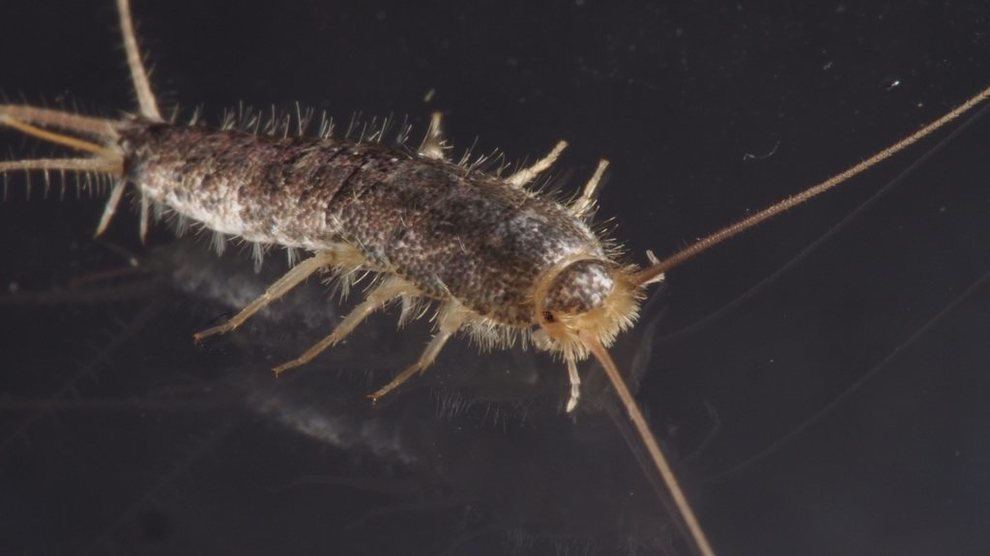
\includegraphics[width=4.16667in,height=\textheight]{skjeggkre.jpg}
\caption{Long-tailed silverfish (\emph{Ctenolepisma longicaudata}). Photo: Johan Mattson.}
\end{figure}

To your dismay, you discover that a population of long-tailed silverfish (``Skjeggkre'', \emph{Ctenolepisma longicaudata}) has moved into your apartment. After some initial investigations, you find out that the population grows by approximately \(1\%\) each day.

\begin{enumerate}
\def\labelenumi{\arabic{enumi}.}
\item
  What is the value of \(\lambda\) for this population? What is the time unit?
\item
  How long will it take for the population to double in size?
\item
  If the current population size is 100 individuals, how large will it be after one year - assuming nothing is stopping its growth? Make a plot of the population growth over this period.
\end{enumerate}

\hypertarget{s02-life-tables}{%
\chapter{Life tables}\label{s02-life-tables}}

A \textbf{life table} is an important tool in demography, helping us keep track of birth and death rates of individuals across age or age groups. Life tables are used extensively in human demography, social sciences, and epidemiology, for instance to calculate the remaining life expectancy at each age, and to project future mortality rates. In life history theory, which aims to understand the evolution of different life history strategies, life tables are used to calculate important parameters for ecological and evolutionary dynamics, such as the net reproductive rate \(R_0\) and the long-term population growth rate \(\lambda\).

Life tables are closely connected to age-structured matrix models and life cycle graphs (chapter \ref{s03-MatrixModels}) - these are all different representations of the life history of a given population. While life tables are useful for manual calculations, matrix models are the most efficient way to do life history calculations, and have several additional useful properties. Matric models are also able to describe with many different kinds of structure beyond age structure.

\hypertarget{learning-goals-1}{%
\section{Learning goals}\label{learning-goals-1}}

\begin{itemize}
\item
  Define life tables, explain the difference between a dynamic and static life table.
\item
  Perform simple life table calculations (e.g.~net reproductive rate \(R_0\), generation time \(T_C\)).
\item
  Write the Euler-Lotka equation for a given life table and explain how it can be solved to find the long-term growth rate \(\lambda\).
\item
  Discuss the advantages and disadvantages of different fitness measures.
\item
  Explain how life tables can be used to study the evolution of different life history strategies, including semelparity/iteroparity and clutch size.
\end{itemize}

\hypertarget{age-specific-survival-and-fecundity}{%
\section{Age-specific survival and fecundity}\label{age-specific-survival-and-fecundity}}

Before going into the life table methods in detail, this section will introduce the basic concepts of age-specific survival and fecundity, as well as a brief discussion of life history strategies.

One of the most basic ways to describe the life history of a population, is through the age-specific probability of survival and fecundity (average number of offspring produced per individual). The \textbf{survivorship} \(l_x\) is the survival probability from birth (age 0) to age \(x\), where \(l_0=1\) by definition. If we follow a cohort of individuals from their birth until all are dead, and record the number of individuals \(n_x\) still alive in the cohort at each age \(x\), then \(l_x\) is given by \(n_x/n_0\).

If we plot \(l_x\) against age \(x\), this curve will always (eventually) decline to zero, as no individual can survive forever (although some species are almost immortal). However, the way in which the curve declines contains important information about the life history of the population. It is common to distinguish between three main types of survivorship curves (on log scale, fig \ref{fig:fig1}): With \emph{type I} curves, \(\ln l_x\) declines very slowly for young ages, but rapidly at old age. This kind of survival is typical for many long-lived mammals, including humans and elephants. With \emph{type II} curves, \(\ln l_x\) declines linearly with age, which means that the mortality is constant and age-independent. This pattern is typical for some birds and smaller mammals. With \emph{type III} , the \(\ln l_x\) curve declines very rapidly in the beginning (for the youngest ages), and then slowly, which is a typical pattern for many trees (producing seeds that have high mortality rates) and fish.

\begin{figure}
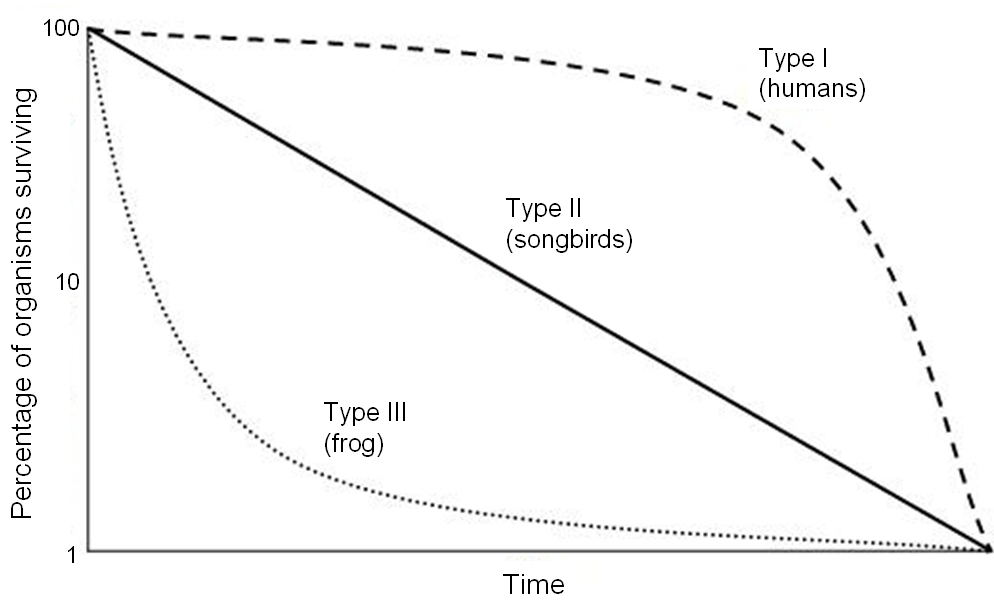
\includegraphics[width=0.7\linewidth]{Survivorship_Curves} \caption{Three main types of survivorship curves (note the log scale on y-axis). Credit: Rayhusthwaite at English Wikipedia / CC-BY (https://creativecommons.org/licenses/by/3.0)}\label{fig:fig1}
\end{figure}

The \textbf{annual survival probability} \(p_x\) is the probability of survival from from age \(x\) to age \(x+1\). The survivorship probability \(l_x\) is related to the annual survival probability \(p_x\) as

\begin{align}
\begin{split}
l_0&=1\\
l_x&=l_{x-1}p_{x-1},\,\:x\geq 1.
\end{split}
\label{eq:survival}
\end{align}

The \textbf{fecundity} \(m_x\) is the number of newborn offspring produced by an individual at age \(x\), and fecundity curves (plotting \(m_x\) against age \(x\)) can also contain information about the general life history of the species. For instance, in many mammals fecundity reaches a peak and then declines with age, while in many size-structured organisms with continuous growth fecundity increases continually with age. Before maturation \(m_x\) will be zero, so the first age at which \(m_x\) is positive is also the age at maturation (note that in life history we define this age based on observed reproduction, not on physiological traits of maturity).

\hypertarget{life-history-strategies-and-trade-offs}{%
\section{Life history strategies and trade-offs}\label{life-history-strategies-and-trade-offs}}

\textbf{Life history strategies} refer to the different combinations of \textbf{life history traits} shown by species or populations, summarized in their age-specific survivorship \(l_x\) and fecundity \(m_x\). The life history is a phenotype, and has a genetic and environmental component. There will always be \textbf{trade-offs} among the life history traits, as individuals have limited access to time and resources, and cannot invest in all traits simultaneously (if they could, evolution would lead to `Darwinian demons' being immortal with infinite amount of offspring). At the species level, life history strategies are the combinations of life history traits that optimize \textbf{fitness} for a given environment. There is more than one solution (strategy) to this `'optimization problem'', which is reflected in the wide range of life histories shown across different species.

Evolutionary changes require the combination of a selection pressure and genetic variation for the traits that are under selection. Demographic methods allow us to quantify selection pressures (through sensitivities, as we will see later) - other methods are needed to quantify the genetic variation of the traits. But before we can define selection pressures, we need a relevant measure of fitness, and we need to understand how fitness depends on the life history (\(l_x\) and \(m_x\)). In the next sections we will go through theory and methods providing this important link, as well as methods to calculate key life history parameters and selection pressures.

\hypertarget{a-basic-life-table}{%
\section{A basic life table}\label{a-basic-life-table}}

In its most basic form, a life table is a list of age-specific parameters of survival (survivorship \(l_x\), and annual survival probability \(p_x\)) and fecundity (\(m_x\)):

\begin{longtable}[]{@{}
  >{\raggedright\arraybackslash}p{(\columnwidth - 6\tabcolsep) * \real{0.2500}}
  >{\raggedright\arraybackslash}p{(\columnwidth - 6\tabcolsep) * \real{0.2500}}
  >{\raggedright\arraybackslash}p{(\columnwidth - 6\tabcolsep) * \real{0.2500}}
  >{\raggedright\arraybackslash}p{(\columnwidth - 6\tabcolsep) * \real{0.2500}}@{}}
\toprule()
\begin{minipage}[b]{\linewidth}\raggedright
Age \(x\)
\end{minipage} & \begin{minipage}[b]{\linewidth}\raggedright
Survival probability \(p_x\)
\end{minipage} & \begin{minipage}[b]{\linewidth}\raggedright
Survivorship \(l_x\)
\end{minipage} & \begin{minipage}[b]{\linewidth}\raggedright
Fecundity \(m_x\)
\end{minipage} \\
\midrule()
\endhead
0 & \(p_0\) & \(l_0=1\) & \(m_0\) \\
1 & \(p_1\) & \(l_1=p_0\) & \(m_1\) \\
2 & \(p_2\) & \(l_2=l_1p_1\) & \(m_2\) \\
\(\vdots\) & \(\vdots\) & \(\vdots\) & \(\vdots\) \\
k & \(p_k=0\) & \(l_k=l_{k-1}p_{k-1}\) & \(m_k\) \\
\bottomrule()
\end{longtable}

No individual lives past the final age, so the annual survival probability in the final age class is \(p_k=0\). However, before they die, individuals in this final class can produce \(m_k\) offspring on their \(k\)'th birthday. The fecundity will also be zero for the first age classes, until the age of maturation (by definition the first age at which offspring are reproduced).

For sexual species, life tables are often defined only for the female subpopulation, under the assumption that survival and reproduction of females are not influenced by the males. If this assumption holds, the male and female subpopulation will grow with the same rate \(\lambda\), and it does not matter which of the subpopulations we use to describe population growth. However, if female reproduction or survival is limited by the number of males, more complex two-sex models are needed to describe the population growth \citep[see e.g.][]{Caswell1}. We will not consider such models here.

Assuming the life table applies to females only, the fecundity parameter \(m_x\) represents the number of female offspring per female, unless it is specifically mentioned that it includes both male and female offspring. In that case we still need to find the number of female offspring, which is the relevant number for the life table. This depends on the offspring sex ratio. If the offspring sex ratio is 1:1, the number of female offspring is simply the number of offspring divided by 2.

\hypertarget{bird}{%
\subsection{Songbird example}\label{bird}}

\begin{figure}
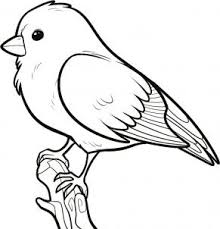
\includegraphics[width=0.3\linewidth]{Songbird2} \caption{A songbird.}\label{fig:fig2}
\end{figure}

As an example, consider a songbird that can live up to 3 years, then reproduces for the last time and dies before reaching age 4. The life table for the female population is given by

\begin{table}

\caption{\label{tab:tablebird}Life table for the bird example.}
\centering
\begin{tabular}[t]{ccccc}
\toprule
Age x & mx & lx & px & lxmx\\
\midrule
0 & 0 & 1.000 & 0.2 & 0.000\\
1 & 0 & 0.200 & 0.9 & 0.000\\
2 & 3 & 0.180 & 0.6 & 0.540\\
3 & 6 & 0.108 & 0.0 & 0.648\\
\bottomrule
\end{tabular}
\end{table}

The final column of this life table lists the product of survivorship and fecundity, \(l_xm_x\), and represents the expected number of offspring that an age 0 individual will produce at each age through life. This product occurs in the calculations of \(R_0\), \(T_C\) and \(\lambda\), and it is therefore often useful to include a separate column for it. We will get back to this example throughout this and the next chapter, and some of the R code builds on previous code for this example. Collected parameters and results for this example are provided in appendix \ref{s07-Code-Collection}. Copy paste this if you want to run later code chunks for the bird example alone without running all the previous code chunks (you still need to define the relevant R functions).

To produce this life table in R, and plot the columns, we can use the following code:

\begin{Shaded}
\begin{Highlighting}[]
\NormalTok{x }\OtherTok{\textless{}{-}} \DecValTok{0}\SpecialCharTok{:}\DecValTok{3} \CommentTok{\#Age}
\NormalTok{k }\OtherTok{\textless{}{-}} \FunctionTok{length}\NormalTok{(x) }
\NormalTok{px }\OtherTok{\textless{}{-}} \FunctionTok{c}\NormalTok{(.}\DecValTok{2}\NormalTok{, .}\DecValTok{9}\NormalTok{, .}\DecValTok{6}\NormalTok{, }\DecValTok{0}\NormalTok{) }\CommentTok{\#Annual survival probability}
\NormalTok{lx }\OtherTok{\textless{}{-}} \FunctionTok{c}\NormalTok{(}\DecValTok{1}\NormalTok{, }\FunctionTok{cumprod}\NormalTok{(px)[}\SpecialCharTok{{-}}\NormalTok{k]) }\CommentTok{\#survivorship }
\NormalTok{mx }\OtherTok{\textless{}{-}} \FunctionTok{c}\NormalTok{(}\DecValTok{0}\NormalTok{, }\DecValTok{0}\NormalTok{, }\DecValTok{3}\NormalTok{, }\DecValTok{6}\NormalTok{) }\CommentTok{\#Fecundity}

\NormalTok{songbird.lifetable }\OtherTok{\textless{}{-}} \FunctionTok{data.frame}\NormalTok{(}\StringTok{"x"} \OtherTok{=}\NormalTok{ x, }\StringTok{"lx"}\OtherTok{=}\NormalTok{lx, }\StringTok{"px"}\OtherTok{=}\NormalTok{px, }\StringTok{"mx"}\OtherTok{=}\NormalTok{mx, }\StringTok{"lxmx"}\OtherTok{=}\NormalTok{lx}\SpecialCharTok{*}\NormalTok{mx)}

\CommentTok{\#For plotting it is useful to use the long format:}
\NormalTok{songbirds.long }\OtherTok{\textless{}{-}}\NormalTok{ songbird.lifetable }\SpecialCharTok{\%\textgreater{}\%} \FunctionTok{pivot\_longer}\NormalTok{(}\FunctionTok{c}\NormalTok{(lx, px,  mx,lxmx),}
               \AttributeTok{names\_to =} \StringTok{"VitalRates"}\NormalTok{, }\AttributeTok{values\_to =} \StringTok{"Value"}\NormalTok{)}
 
\FunctionTok{ggplot}\NormalTok{(songbirds.long) }\SpecialCharTok{+} 
  \FunctionTok{geom\_line}\NormalTok{(}\FunctionTok{aes}\NormalTok{(}\AttributeTok{x=}\NormalTok{x,}\AttributeTok{y=}\NormalTok{Value ),}\AttributeTok{col=}\DecValTok{1}\NormalTok{, }\AttributeTok{lwd=}\FloatTok{1.2}\NormalTok{)}\SpecialCharTok{+}
  \FunctionTok{facet\_wrap}\NormalTok{(}\SpecialCharTok{\textasciitilde{}}\FunctionTok{factor}\NormalTok{(VitalRates,}\AttributeTok{levels=}\FunctionTok{c}\NormalTok{(}\StringTok{"px"}\NormalTok{, }\StringTok{"lx"}\NormalTok{ , }\StringTok{"mx"}\NormalTok{, }\StringTok{"lxmx"}\NormalTok{)), }\AttributeTok{scales=}\StringTok{"free"}\NormalTok{)}\SpecialCharTok{+}
  \FunctionTok{theme\_bw}\NormalTok{() }\SpecialCharTok{+}
  \FunctionTok{labs}\NormalTok{( }\AttributeTok{x=}\StringTok{"Age (year)"}\NormalTok{, }\AttributeTok{y=}\StringTok{"Value"}\NormalTok{)}
\end{Highlighting}
\end{Shaded}

\begin{figure}
\centering
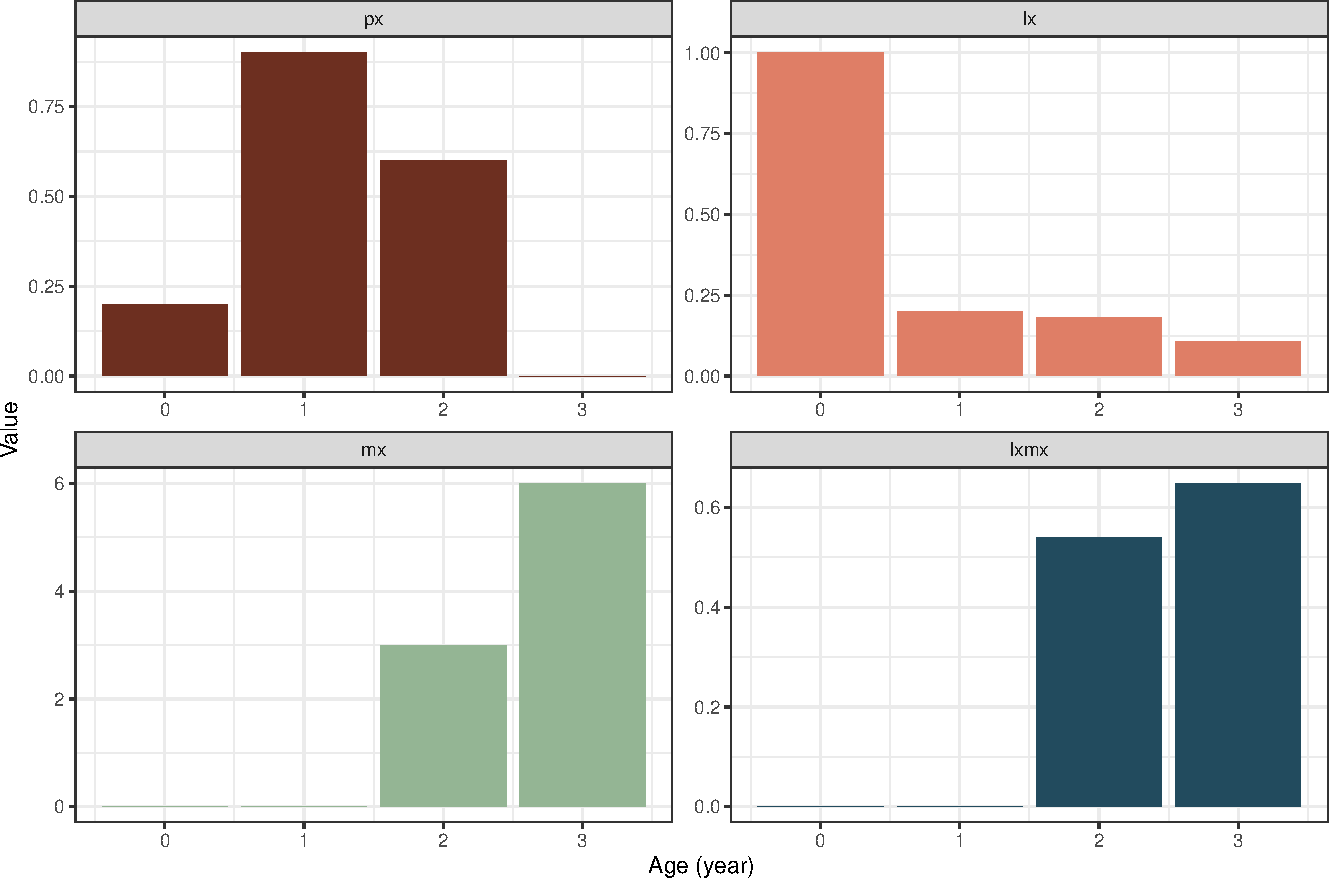
\includegraphics{DemographyCompendium_files/figure-latex/figbird1-1.pdf}
\caption{\label{fig:figbird1}Plot of columns from the songbird life table (table \ref{tab:tablebird}): Age-specific survivorship \(l_x\), annual survival \(p_x\), fecundity \(m_x\), and the product \(l_xm_x\).}
\end{figure}

\hypertarget{dynamic-and-static-life-tables}{%
\section{Dynamic and static life tables}\label{dynamic-and-static-life-tables}}

There are two main ways of collecting data and estimating the age-specific parameters of survival and reproduction in a population. With a \emph{dynamic life table}, also known as a cohort life table, an entire cohort of individuals are followed from birth to death, and their survivorship and fecundity is recorded at each age. This approach is often expensive and time-demanding, and in many cases it is not practically possible to obtain such data. The other main approach is the \emph{static life table}, which is based on recording the survival and reproduction of individuals from the whole population (all age groups) over one or a few time steps. This approach is usually more feasible, and corresponds to taking a cross-section of the population at a given time. However, the approach assumes that we are able to determine the age of individuals, which is difficult in many species. In many studies, more coarse age classifications such as ``juvenile'' or ``adult'' are used.

Importantly, the static life table approach is based on the assumptions that 1) the population is stationary (constant or near constant population size over time), and 2) the population has a stable age structure (the proportions of individuals in each age class do not change over time). A dynamic and static life table for a given population will be the same if the age-specific parameters of survival and fecundity are constant over time. For real populations this is rarely the case, but the life tables can still provide a good approximation.

\hypertarget{empirical-data-in-demography}{%
\subsubsection*{Empirical data in demography}\label{empirical-data-in-demography}}
\addcontentsline{toc}{subsubsection}{Empirical data in demography}

To get reliable empirical estimates of mean survival and fecundity we need long-term individual-based data. Incorporating effects of climate change and other external changes requires even longer time series, as some environmental events occur only rarely but can have large impact on the population.

Study systems providing such detailed long-term data from wild populations are rare, and require much effort to maintain. Those we have are extremely valuable, and much of our ecological and evolutionary knowledge is derived from these study systems.

\hypertarget{life-table-calculations}{%
\section{Life table calculations}\label{life-table-calculations}}

Once we have a life table with columns representing age, survivorship and fecundity, several useful quantities can be calculated. We will focus on three of them: The net reproductive rate \(R_0\), the cohort generation time \(T_C\), and the long-term growth rate \(\lambda\).

All of these quantities can also be calculated directly from a projection matrix, as we will see later (chapter @ref(\#s03-MatrixModels)).

\hypertarget{net-reproductive-rate}{%
\subsection{Net reproductive rate}\label{net-reproductive-rate}}

The \textbf{net reproductive rate} represents the number of female offspring by which each female will be replaced over her lifetime, on average, and is also known as the lifetime reproductive sucess:

\begin{align}
R_0=\sum_{x=0}^k l_xm_x.
\label{eq:R0}
\end{align}

The product \(l_xm_x\) represents the number of offspring produced at age \(x\) given that the individual survives to that age. Thus, summing up this product for all ages we get the net reproductive rate.

The net reproductive rate is a measure of the population growth rate per generation. For instance, if \(R_0=1.1\) the population will grow by 10\% each generation. Thus, \(R_0\) holds information on the population growth rate \(\lambda\), although the two are not the same (\(\lambda\) is per time step, while \(R_0\) is per generation). If \(R_0>1\), we know that the population is growing (\(\lambda>1\)), if \(R_0=1\) then \(\lambda=1\) and the population is stable, and if \(R_0<1\) then \(\lambda<1\), and the population is declining.

\hypertarget{bird-example}{%
\subsubsection*{Bird example}\label{bird-example}}
\addcontentsline{toc}{subsubsection}{Bird example}

From the bird life table (table \ref{tab:tablebird}), we see that the age at first reproduction is 2, and that although few individuals live to age 3, this is the age class of highest expected number of offspring. The net reproductive rate is in this case

\[
R_0=\sum_{x=0}^3 l_xm_x=0+0+0.54+0.648=1.188.
\]
Thus, each female is expected to be replaced by 1.188 female offspring on average. From this number we now know that the population is growing (\(\lambda>1\) since \(R_0>1\)), although we do not yet know the value of the population growth rate \(\lambda\).

In R, we can find this from the life table (or the vectors) as follows:

\begin{Shaded}
\begin{Highlighting}[]
\NormalTok{R0.lifetable }\OtherTok{\textless{}{-}} \ControlFlowTok{function}\NormalTok{(lx, mx)\{}
  \FunctionTok{sum}\NormalTok{(lx}\SpecialCharTok{*}\NormalTok{mx) }
\NormalTok{\}}

\CommentTok{\#Bird example:}
\NormalTok{R0\_Bird }\OtherTok{\textless{}{-}} \FunctionTok{R0.lifetable}\NormalTok{(lx, mx) }
\NormalTok{R0\_Bird}
\end{Highlighting}
\end{Shaded}

\begin{verbatim}
## [1] 1.188
\end{verbatim}

Note that R automatically multiplies each element of the vectors first, before summing the products.

\hypertarget{cohort-generation-time}{%
\subsection{Cohort generation time}\label{cohort-generation-time}}

The generation time reflects the `pace of life' of a species. Many biological properties (physiological rates, other life history parameters) scale with generation time. For age structured populations with overlapping generations there are different ways to define generation time. We will use the socalled \textbf{cohort generation time}, which is the mean age at reproduction of all the \(R_0\) offspring the average individual produces:

\begin{align}
T_C=\frac{1}{R_0}\sum_{x=0}^{k} xl_xm_x.
\label{eq:Generation}
\end{align}

The expression \(xl_xm_x/R_0\) represents the fraction of the mean lifetime reproduction (\(R_0\)) that happens at age \(x\). By summing this up for all ages (and moving 1/\(R_0\) outside the sum) we get the average age at which reproduction occurs.

\hypertarget{bird-example-1}{%
\subsubsection*{Bird example}\label{bird-example-1}}
\addcontentsline{toc}{subsubsection}{Bird example}

Using the measure defined above and the values in table \ref{tab:tablebird}, the cohort generation time for the songbird is given by

\[
T_C=\frac{1}{R_0}\sum_{x=0}^k xl_xm_x=\frac{1}{1.188} (0+0+2\cdot0.54+3\cdot0.648)=2.54.
\]

In R, we can find this as follows:

\begin{Shaded}
\begin{Highlighting}[]
\NormalTok{TC.lifetable }\OtherTok{\textless{}{-}} \ControlFlowTok{function}\NormalTok{(x, lx, mx)\{}
\NormalTok{  R0 }\OtherTok{\textless{}{-}} \FunctionTok{R0.lifetable}\NormalTok{(}\AttributeTok{lx=}\NormalTok{lx, }\AttributeTok{mx=}\NormalTok{mx)}
  \FunctionTok{sum}\NormalTok{(x}\SpecialCharTok{*}\NormalTok{lx}\SpecialCharTok{*}\NormalTok{mx)}\SpecialCharTok{/}\NormalTok{R0\_Bird}
\NormalTok{\}}

\CommentTok{\#Bird example:}

\NormalTok{TC\_Bird }\OtherTok{\textless{}{-}} \FunctionTok{TC.lifetable}\NormalTok{(x,  lx, mx)}

\NormalTok{TC\_Bird}
\end{Highlighting}
\end{Shaded}

\begin{verbatim}
## [1] 2.545455
\end{verbatim}

\hypertarget{approximation-of-long-term-growth-rate}{%
\subsection{Approximation of long-term growth rate}\label{approximation-of-long-term-growth-rate}}

Since \(R_0\) is an estimate of the per generation growth rate and \(T_C\) an estimate of generation time, we can use them to estimate the population growth rate per time step, the intrinsic growth rate \(r\) (see chapter \ref{s01-Exponential} on exponential growth):

\begin{align}
\ln\lambda = r \approx \frac{\ln R_0}{T_C}.
\label{eq:R0T}
\end{align}

This approximation assumes that all offspring produced during the lifetime on average (\(R_0\)) are produced exactly at age \(T_C\), rather than at different ages. It can be a good starting point for the more accurate calculation of \(\lambda\) based on the Euler-Lotka equation, which is the topic of the next section.

\hypertarget{bird-example-2}{%
\subsubsection*{Bird example}\label{bird-example-2}}
\addcontentsline{toc}{subsubsection}{Bird example}

Using the values calculated above, we get the following approximation of \(\lambda\) for the songbird:

The estimate of \(\lambda\) based on \(R_0\) and \(T_C\) is given by
\[
\lambda\approx e^{\ln R_0/T_C}=e^{\ln 1.188/2.54}\approx 1.07.
\]

In R, we can find this as follows, using the bird example:

\begin{Shaded}
\begin{Highlighting}[]
\FunctionTok{exp}\NormalTok{(}\FunctionTok{log}\NormalTok{(R0\_Bird)}\SpecialCharTok{/}\NormalTok{TC\_Bird)}
\end{Highlighting}
\end{Shaded}

\begin{verbatim}
## [1] 1.070021
\end{verbatim}

\hypertarget{Euler}{%
\subsection{Euler-lotka equation}\label{Euler}}

The \textbf{Euler-Lotka equation} is an essential equation in life history theory, because it provides the link between the life history of the focal population, as described by the age-specific fecundity \(m_x\) and survivorship \(l_x\), and the mean fitness \(\lambda\) (long-term population growth rate), associated with that life history.

To derive the Euler-Lotka equation, we first define the number of newborn individuals at time \(t\), which is the sum of the newborns produced at each age:

\begin{align}
n_0(t)=\sum_{x=0}^{k}n_0(t-x)l_xm_x.
\label{eq:Euler1}
\end{align}

Here, \(n_0(t-x)\) is the number of newborn \(x\) years ago (that are now aged \(x\) years). This number is multiplied by \(l(x)\) to obtain the number of them that are still alive at age \(x\), and then by \(m(x)\) to get the total number of offspring they produce at age \(x\). The sum is over all ages, to get the total number of offspring (left side of the equation). For the next step of the derivation, we first assume that the population, and therefore each age class, grows steadily and exponentially at rate \(\lambda\). Because the population grows exponentially, we assume that the number of newborn over time will follow an equation on the form \(n_0(t)=Q\lambda^t\) (remember the equation for exponential growth), where \(Q\) is an unknown constant. Inserting this for \(n_0(t)\) and \(n_0(t-x)\) in the equation above, we now get

\begin{align}
Q\lambda^{t}=\sum_{x=0}^{k}Q\lambda^{t-x}l_xm_x.
\label{eq:Euler2}
\end{align}

Finally, we divide each side by \(Q\lambda^t\) to get the Euler-Lotka equation (remember that we can write \(\lambda^{t-x}=\lambda^{t}\lambda^{-x}\)):

\begin{align}
1=\sum_{x=0}^{k}\lambda^{-x}l_xm_x.
\label{eq:Euler}
\end{align}

It is now tempting to try to rearrange this equation to isolate \(\lambda\) on one side, to get a `nice' expression for \(\lambda\) as a function of the
cumulative survival and fecundity. Unfortunately, this is not possible (except for a few special cases)! This equation can only be solved numerically, for instance by trial and error (change the value of \(\lambda\) in the expression until you find the one that leads to the sum being close to 1).

\hypertarget{bird-example-3}{%
\subsubsection*{Bird example}\label{bird-example-3}}
\addcontentsline{toc}{subsubsection}{Bird example}

The exact value of \(\lambda\) is defined by the Euler-Lotka equation, which for the bird example (table\ref{tab:tablebird}) is given by

\[
1=\sum_{x=0}^{k}\lambda^{-x}l_xm_x=0.54\lambda^{-2}+0.648\lambda^{-3}.
\]
We can solve this by trial and error, and a good starting value for \(\lambda\) is the estimate from \(R_0\) and \(T_C\), \(\lambda \approx1.07\). However, solving the equation is more easily done in R.

One of several possible approaches is to use the function \texttt{uniroot()}. You are not expected to memorize the details of this approach, but it is shown here as it can be useful with lifetables. Uniroot searches for the solution of a function (i.e.~the value of its first argument that makes the expression in the function equal to zero) within a predefined range. For this to work for the Euler-Lotka equation, we need to rearrange it to get an expression that equals zero (just move the number 1 from right-hand side to left hand side), make sure \(\lambda\) is the first argument of this function, and then apply the uniroot function:

\begin{Shaded}
\begin{Highlighting}[]
\CommentTok{\#Rearranging the Euler{-}Lotka function to get an expression equal to zero:}
\NormalTok{EulerLotka }\OtherTok{\textless{}{-}} \ControlFlowTok{function}\NormalTok{(lambda, x, lx, mx)\{}
  \FunctionTok{sum}\NormalTok{(lambda}\SpecialCharTok{\^{}}\NormalTok{(}\SpecialCharTok{{-}}\NormalTok{x)}\SpecialCharTok{*}\NormalTok{lx}\SpecialCharTok{*}\NormalTok{mx)}\SpecialCharTok{{-}}\DecValTok{1}
\NormalTok{\}}

\CommentTok{\#Define search range for lambda in uniroot}
\NormalTok{lambda.range }\OtherTok{\textless{}{-}} \FunctionTok{c}\NormalTok{(.}\DecValTok{1}\NormalTok{,}\DecValTok{2}\NormalTok{)}

\CommentTok{\#Apply uniroot to find lambda, store the result}
\NormalTok{lambdabird }\OtherTok{\textless{}{-}} \FunctionTok{uniroot}\NormalTok{(EulerLotka, }\AttributeTok{x=}\NormalTok{x, }\AttributeTok{lx=}\NormalTok{lx, }\AttributeTok{mx=}\NormalTok{mx, }\AttributeTok{interval=}\NormalTok{lambda.range)}\SpecialCharTok{$}\NormalTok{root}
\end{Highlighting}
\end{Shaded}

With this approach the estimated value is \(\lambda=\) 1.07025, close to the approximated value calculated above.

You have now seen an example of how the Euler-Lotka equation can be solved in R, but this approach is not commonly used. It is much more convenient to find \(\lambda\) based on the projection matrix from a matrix model, which is the topic of section \ref{s03-MatrixModels}.

\hypertarget{fitness-measures-in-life-history-theory}{%
\section{Fitness measures in life history theory}\label{fitness-measures-in-life-history-theory}}

In the context of life history theory, fitness is often measured by the long-term growth rate \(\lambda\) (or equivalently \(r=\ln\lambda\)) as defined by the Euler-Lotka equation, or by the dominant eigenvalue of the projection matrix (chapter \ref{s03-MatrixModels}).

Another fitness measure which is commonly used, is the lifetime reproductive success, \(R_0\) (equation \eqref{eq:R0}). This measure does however not account for timing of life history events (at which ages reproduction happens, for instance), and thus ignores an important aspect of the life history. Both \(\lambda\) and \(R_0\) are based on the assumption of constant age-specific survival and fecundity in the life table, and neither is a good measure of fitness in the case of strong density- or frequency-dependence (because \(\lambda\) and \(R_0\) are both based on average values that are not useful for understanding selection in such situations). Life history theory deals mostly with outcomes of evolutionary processes in the long run (i.e.~evolution of entire life histories) and to a less extent the short-term dynamics of gene frequencies (population genetics). With strong density or frequency dependence, and where the purpose is to estimate gene frequencies over time, other methods are better suited (e.g.~adaptive dynamics frameworks). These are not considered here, but note that the measure of fitness will also generally be different in these cases.

Following the convention through most of the literature on life history evolution and quantitative genetics based on demographic models, \(\lambda\) is the main fitness measure for a structured population in a constant environments.

\hypertarget{semelparity-and-iteroparity}{%
\section{Semelparity and iteroparity}\label{semelparity-and-iteroparity}}

Some species, including most mammals, have multiple reproductive events during their lifetime. This is known as \textbf{iteroparity}, while \textbf{semelparity} applies to species that reproduce only once. This mode of reproduction is used by annual plants as well as some perennials, several invertebrates, many fish species, and a few mammals. In salmon, some species are iteroparous and others are semelparous. From a life history perspective it is interesting to know under which circumstances evolution of iteroparity versus semelparity is favored, and we can use the knowledge from life table methods to investigate this question.

\citet{Cole1} was among the authors who were interested in this and other life history questions. He is known for \textbf{Cole's paradox}, which was only a small part of a larger article. In this example, Cole compared two species: The first is semelparous and lives for only a year, after which it produces \(m_1\) offspring and dies. The second is iteroparous and lives forever (survival probability of 1 each year), producing \(m_2\) offspring each year. Now look at the annual growth rate (fitness) \(\lambda\) for each species: Species 1 gets \(\lambda_1=m_1\) (since each individual leaves behind \(m_1\) individuals on average each year), while the second species gets \(\lambda_2=1+m_2\) (each individual leaves behind \(1+m_2\) individuals each year, i.e.~itself plus offspring). What would it take for the semelparous species to have higher fitness than the iteroparous one?

\begin{align}
\lambda_1 > \lambda_2\\
m_ 1> 1+m_2.
\end{align}

In other words, as long as the semelparous species (species 1) produces at least 1 more offspring per clutch than the iteroparous one (species 2), it would have the same or higher fitness. This is known as Cole's paradox, as it seems unlikely that an immortal species should get the same fitness as a mortal one having just one more offspring per clutch. It is also a paradox that semelparity is not more common (in birds an mammals) if semelparity is so `cheap' to evolve. The clue to `resolve' the paradox is that the assumptions for each species are too simplistic to apply to the real world. Once we take more realism into account, for instance drop immortality but instead have an annual survival probability \(p<1\) for the iteroparous species, and introduce a difference between adults and juveniles (where juveniles cannot reproduce), iteroparity becomes relatively more favorable and it would cost more to switch to a semelparous life history.

Note that while semelparity is `rare' in birds and mammals, which likely motivated the need to explain how it evolved (compared to iteroparity), it is common in other taxa.

\hypertarget{the-lack-clutch}{%
\section{The Lack clutch}\label{the-lack-clutch}}

The concept of the \textbf{Lack clutch} originates from ornithology, but applies generally to other organisms as well. It is named after the ornithologist David Lack, who suggested a pioneering baseline model for understanding life history trade-offs that affect clutch size.

The problem started from the observation, including brood manipulation studies, that many birds seem to lay fewer eggs per clutch than they could manage to raise to fledging (independence). This suggests there could be one or more life history trade-offs constraining birds from laying larger clutches, and that the observed clutch size perhaps represents some fitness optimum for the current environment. Lack's model assumes that this trade-off is with fledgling survival, and he also assumed this trade off was linear. In that case, the optimum clutch size, from the parent's point of view, is the one that maximizes the number of offspring that survive to fledging. This clutch size is known as the Lack clutch. Each offspring, on the other hand, would prefer (from a fitness perspective) to have all parental effort to itself, so that the optimum clutch size from the offspring point of view is 1. This is an example of a \textbf{parent-offspring conflict} (where offspring and parents do not `agree', evolutionarily speaking, on what is the optimum parental investment in a clutch).

We can describe the Lack clutch model mathematically as follows. Let \(N_e\) be the number of eggs laid in a clutch, and let \(l_f(N_e)\) be the probability of survival from egg laying until fledging (when offspring are independent). It is a linear function of the number of eggs in the clutch:

\begin{align}
l_f(N_e)=1-cN_e,
\end{align}
where \(c\) is the slope of the relationship. The number of survived fledglings is then given by

\begin{align}
N_f(N_e)&=l_f(N_e)N_e\\
&=(1-cN_e)N_e\\
&=N_e-cN_e^2.
\end{align}

This is a quadratic function, and we find the maximum (or minimum) where the derivative is equal to zero. The corresponding value of \(N_e\) is the Lack clutch \(N_e^*\):

\begin{align}
\frac{dN_f(N_e)}{dN_e}&=1-2cN_e\\
1-2cN_e^*&=0\\
N_e^*=\frac{1}{2c}.
\end{align}

This tells us that the stronger the trade-off with offspring survival (size of the slope \(c\)), the lower the Lack clutch size. The Lack clutch is larger than one only for \(c<0.5\).

The Lack clutch is based on a simple model, with some important assumptions that do not necessarily hold for real world examples. The model considers only one (but important) trade-off: Clutch size versus offspring survival until fledging. However, other trade-offs could also affect the clutch size, such as parental survival and future reproduction. Another important assumption is that the trade-off between offspring survival and clutch size is linear, but this is just a convenient assumption. In many cases the offspring survival could be a non-linear function of clutch size (for instance if parasitism affects large clutches more than small ones). Furthermore, the model assumes a constant environment, and that parents treat all offspring of the clutch equally. In many species, for instance in many raptors, parents favor the largest / oldest of the siblings, so that younger siblings only survive in very good conditions (or if the older ones die for some reason). In these cases, the younger offspring may represent an ``insurance'' for the parents, and effects like this are not captured in the simple Lack clutch model. Still, this is a good baseline model for exploration of more complex hypotheses around the evolution of clutch size.

\hypertarget{exercises-1}{%
\section{Exercises}\label{exercises-1}}

For suggested solutions, see appendix \ref{s09-Solutions}.

\hypertarget{exercise-2.1}{%
\subsection*{Exercise 2.1}\label{exercise-2.1}}
\addcontentsline{toc}{subsection}{Exercise 2.1}

The table shows the average lifetime number of children per woman in some different countries.

\begin{table}

\caption{\label{tab:table21}Average lifetime number of children in different countries (2019 data from http://worldpopulationreview.com/countries/total-fertility-rate/).}
\centering
\begin{tabular}[t]{cc}
\toprule
Country & Children per woman\\
\midrule
Mali & 5.8\\
Tunisia & 2.2\\
Australia & 1.7\\
Norway & 1.6\\
South Korea & 0.9\\
\bottomrule
\end{tabular}
\end{table}

Assume exponential growth, and use the approximation in equation \eqref{eq:R0T} to answer the questions:

\begin{enumerate}
\def\labelenumi{\arabic{enumi}.}
\item
  What is the annual population growth rate (\(\lambda\)) of each country, given different assumptions for the value of generation time?
\item
  How many years does each country need to double in population size, if we assume a generation time of 25 years?
\item
  How well / poorly do you think these populations meet the assumptions made for these calculations?
\end{enumerate}

\hypertarget{exercise-2.2}{%
\subsection*{Exercise 2.2}\label{exercise-2.2}}
\addcontentsline{toc}{subsection}{Exercise 2.2}

\begin{figure}

\includegraphics[width=0.4\linewidth]{plant} \caption{Flowering plant}\label{fig:plant}
\end{figure}

A botanist follows a cohort of a flowering plant from seeds (age 0) until all are dead. He marks the seedlings and comes back every year and counts how many living plants are remaining in the cohort. When they start to reproduce he counts the number of seeds per plant. Based on this information he writes the following incomplete life table:

\begin{table}

\caption{\label{tab:unnamed-chunk-6}Incomplete life table for a flowering plant.}
\centering
\begin{tabular}[t]{c|c|c}
\hline
Age $x$ & Remaining cohort $n_x$ & Fecundity $m_x$\\
\hline
0 & 12376 & 0.0\\
\hline
1 & 4233 & 0.0\\
\hline
2 & 1790 & 0.0\\
\hline
3 & 340 & 2.1\\
\hline
4 & 268 & 3.2\\
\hline
\end{tabular}
\end{table}

\begin{enumerate}
\def\labelenumi{\arabic{enumi}.}
\item
  What is the age at first reproduction of this plant?
\item
  Create the same life table in R, with columns corresponding to Age \(x\), Remaining cohort \(n_x\), and fecundity \(m_x\).
\item
  Calculate the vectors of cumulative survival probability \(l_x\) and annual survival probability \(p_x\), and add these as columns to the life table you created.
\item
  Make plots of each life table column (\(n_x\), \(l_x\), \(p_x\), \(m_x\)) as a function of age \(x\). Describe the life history you see from the plot.
\item
  Calculate the mean lifetime reproduction \(R_0\) from the life table. What does this value say about the population growth rate?
\item
  Calculate the generation time \(T_C\) from the life table. What does this measure actually describe? What is the estimate of \(\lambda\) based on \(R_0\) and \(T_C\)?
\item
  Solve the Euler-Lotka equation for \(\lambda\) using the method demonstrated for the bird example. How does this value of \(\lambda\) differ from the estimate based on \(R_0\) and \(T_C\)?
\end{enumerate}

\hypertarget{exercise-2.3}{%
\subsection*{Exercise 2.3}\label{exercise-2.3}}
\addcontentsline{toc}{subsection}{Exercise 2.3}

\begin{enumerate}
\def\labelenumi{\arabic{enumi}.}
\item
  In the bird example (section \ref{bird}), the values of fecundity given in table \ref{tab:tablebird} correspond to the mean number of fledged female offspring per adult female. Assume that the offspring survival (from eggs to fledging) is 0.9, what is the average clutch size (number of eggs laid) at each age?
\item
  If we assume that the assumptions of the Lack clutch apply, what is the trade-off between offspring survival and offspring number at each age?
\item
  In another bird species, a close relative to this example bird, individuals only reproduce at age 3. Otherwise this species has the same average fitness and the same survivorship as in our bird example. What is the fecundity in this other species?
\item
  What is the name of the reproductive mode of the two bird species (the example bird and its relative)? Discuss why (or why not) the two species fit with the result of Cole's paradox.
\end{enumerate}

\hypertarget{s03-MatrixModels}{%
\chapter{Age-structured matrix population models}\label{s03-MatrixModels}}

Matrix models make it possible to work with systems of multiple equations simultaneously, which is what we need to describe the growth of structured populations. For instance, if we study a long-lived species with 50 age classes, it is very cumbersome to write down the growth equations for all of the 50 age classes. With a matrix model we need only one equation to keep track of the growth of all of stages simultaneously.

This chapter will deal with age-structured matrix models and introduce methods for calculating key properties of life history and population growth. Chapter @ref\{s04-stage\} will introduce more general stage structured models, and we will see that the methods introduced here for age-structured populations are applicable also to these cases.

The main `ingredient' of an age-structured matrix model is the Leslie matrix, which contains all the information necessary to project the growth of each age class over time. Several life history parameters can also be calculated directly from this matrix, including the long-term population growth rate \(\lambda\).

\hypertarget{learning-goals-2}{%
\section{Learning goals}\label{learning-goals-2}}

\begin{itemize}
\item
  Define a Leslie matrix for age-structured populations, and its two main components.
\item
  Explain the differences between a pre- and post-reproductive census.
\item
  Show how a Leslie matrix is related to the life table.
\item
  Draw a life cycle graph and explain how it is related to the Leslie matrix.
\item
  Calculate asymptotic parameters from a matrix model (using projection or eigen analysis), and explain their biological meaning.
\item
  Calculate lifetime reproduction, generation time and life expectancy from the Leslie matrix and its main components.
\item
  Calculate sensitivities and elasticities of \(\lambda\) with respect to projection matrix elements or underlying parameters.
\item
  Do an LTRE analysis to understand the difference in the long-term growth rate in two different environments.
\end{itemize}

\hypertarget{age-structured-growth}{%
\section{Age-structured growth}\label{age-structured-growth}}

In this section we will define the growth of each age class as a function of the annual survival probability and fertility, and introduce the matrix equation to describe this growth. In the next sections we will see how the age-structured matrix model is connected to life tables, and how it can be described by a life cycle graph. The last sections present important calculations that can be done with a matrix model.

We will denote the first class as class 1, the second as class 2, etc., but as we will see in section \ref{census}, the definition of the parameters of survival and reproduction depend on census time (when the population is counted within each time step). To keep track of the number of individuals in each of the age classes over time, we define the following \textbf{population vector} \(\mathbf{n}_t\) of individuals in age class 1 to \(k\):

\begin{align}
\mathbf{n}_t=\left[\begin{matrix} n_1(t) \\ n_2(t)\\ \vdots \\ n_k(t) \end{matrix} \right].
\label{eq:popvec}
\end{align}

The total population size at time \(t\) is the sum of this vector, \(N_t=\sum_{j=1}^kn_j(t)\) (note that we now use \(j\) or \(i\) as index instead of \(x\), following conventional notation for matrix models). Let \(s_j\) describe the survival probability of individuals in age class \(j\) to the next time step, and \(f_j\) the number of offspring produced by each individual in age class \(j\) that enter age class 1 at time \(t+1\). Importantly, \(s_j\) and \(f_j\) of the Leslie matrix are \emph{not the same} as the age-specific survival probability \(p_j\) and fecundity \(m_j\) (see section \ref{census}).

The growth of age class 1 (offspring) from one time step to the next is then given by

\begin{equation}
n_1(t+1)=f_1n_1(t)+f_2n_2(t)+\ldots +f_kn_k(t),
\label{eq:AgeGrowth1}
\end{equation}

while the growth of the other age classes is given by

\begin{align}
\begin{split}
n_2(t+1)&=s_1n_1(t),\\
n_3(t+1)&=s_2n_2(t),\\
\vdots \\
n_k(t+1)&=s_{k-1}n_{k-1}(t).\\
\end{split}
\label{eq:AgeGrowth2}
\end{align}

Together, theses equations constitute a system of linear equations, which we can describe with a matrix model:

\begin{align}
\begin{split}
\mathbf{n}_{t+1}&=\mathbf{A}\mathbf{n}_t\\
\left[\begin{matrix} n_1 \\n_2 \\ \vdots \\  \\ n_k   \\  \end{matrix}\right]_{t+1}&=\left[\begin{matrix} f_1 & f_2 && \cdots & f_k \\ s_1 &0 && \cdots &0\\ 0 &s_2 & &\cdots &0\\ \vdots& &\ddots&&\vdots\\ 0 &\cdots&0 & s_{k-1} &0  \\  \end{matrix}\right]\left[\begin{matrix} n_1 \\n_2 \\ \vdots \\  \\ n_k   \\  \end{matrix}\right]_{t}.
\end{split}
\label{eq:LeslieGrowth}
\end{align}

This is the age-structured version of the exponential growth model of an unstructured population (section \ref{s01-Exponential}). The matrix \(\mathbf{A}\) is a square matrix (same number of rows and columns), of dimension \(k \times k\), where \(k\) is the number of age classes. It is named a \textbf{Leslie matrix} after the work of Leslie \citetext{\citeyear{Leslie1}; \citeyear{Leslie2}}, and the more general term which also applies to other kinds of structure is a \textbf{projection matrix}. The elements of the first row of \(\mathbf{A}\) represent the production of offspring to next year's population from each of the age classes. Here we refer to these elements as \textbf{fertility coefficients} or simply fertilities, while the \textbf{survival coefficients} are located along the sub-diagonal of the Leslie matrix. In the final age class, no individuals survive until the next time step, but individuals can reproduce and contribute with a number \(f_k\) to next year's age class 1.

The Leslie matrix can be decomposed as the sum of a \textbf{survival matrix} \(\mathbf{U}\) and a \textbf{fertility matrix} \(\mathbf{F}\):

\begin{align}
\begin{split}
\mathbf{A}&=\mathbf{U}+\mathbf{F}\\
\left[\begin{matrix} f_1 & f_2 && \cdots & f_k \\ s_1 &0 && \cdots &0\\ 0 &s_2 & &\cdots &0\\ \vdots& &\ddots&&\vdots\\ 0 &\cdots&0 & s_{k-1} &0  \\  \end{matrix}\right] &= \left[\begin{matrix} 0 & 0 && \cdots & 0 \\ s_1 &0 && \cdots &0\\ 0 &s_2 & &\cdots &0\\ \vdots& &\ddots&&\vdots\\ 0 &\cdots&0 & s_{k-1} &0  \\  \end{matrix}\right] \left[\begin{matrix} f_1 & f_2 && \cdots & f_k \\0  &0 && \cdots &0\\ 0 &0 & &\cdots &0\\ \vdots& &\ddots&&\vdots\\ 0 &\cdots&0 & 0 &0  \\  \end{matrix} \right]
\end{split}
\label{eq:LeslieSplit}
\end{align}

These two sub-matrices are used in the calculations of the net reproductive rate \(R_0\) and generation time \(G\) (section \ref{asymptotic}). In chapter \ref{s04-Stage} we will further decompose these two matrices into components describing survival, fertility and stage transitions.

\hypertarget{LeslieR}{%
\subsection{Creating a Leslie matrix in R}\label{LeslieR}}

The following R function creates a Leslie matrix from vectors of survival \(\mathbf{s}\) and fertility \(\mathbf{f}\) (the vectors must have the same length, corresponding to the number of age classes). The final element of the survival vector should be 0 if the model is purely age-structured (otherwise, individuals are allowed to accumulate in the final class, which is a commonly used extension of age structured models).

\begin{Shaded}
\begin{Highlighting}[]
\NormalTok{Create.Amat }\OtherTok{\textless{}{-}} \ControlFlowTok{function}\NormalTok{(Svec, Fvec)\{}
\NormalTok{  k }\OtherTok{\textless{}{-}} \FunctionTok{length}\NormalTok{(Svec)}
\NormalTok{  MatA}\OtherTok{\textless{}{-}} \FunctionTok{matrix}\NormalTok{(}\DecValTok{0}\NormalTok{,k,k)}
\NormalTok{  MatA[}\DecValTok{1}\NormalTok{,] }\OtherTok{\textless{}{-}}\NormalTok{ Fvec }
  \ControlFlowTok{for}\NormalTok{(i }\ControlFlowTok{in} \DecValTok{1}\SpecialCharTok{:}\NormalTok{(k}\DecValTok{{-}1}\NormalTok{))\{}
\NormalTok{    MatA[i}\SpecialCharTok{+}\DecValTok{1}\NormalTok{,i] }\OtherTok{\textless{}{-}}\NormalTok{ Svec[i]}
\NormalTok{  \}}
\NormalTok{  MatA[k,k] }\OtherTok{\textless{}{-}}\NormalTok{ Svec[k] }\CommentTok{\#Allow individuals to accumulate in final class if Svec[k] \textgreater{}0.}
\NormalTok{  MatA}
\NormalTok{  \}}
\end{Highlighting}
\end{Shaded}

\hypertarget{census}{%
\section{Pre- and post-reproductive census}\label{census}}

The Leslie matrix depends on coefficients of fertility, \(f_j\), and survival probabilities \(s_j\). How these coefficients are linked to the life table depends on the \emph{census type} of the matrix model, in other words at what time point the population is counted during each time step For a birth-pulse population (where individuals reproduce once per time step), there are two main census types: Pre- and post-reproductive* census. As the names indicate, they assume that the population is counted either right before (pre) or right after (post) reproduction.

Census time is important because a lot can happen to a population also within the time intervals of the model. The age-specific parameters describing fecundity (\(m_x\)) and survival (\(l_x\), \(p_x\)) as a function of actual age \(x\) are the same regardless of census time. But the fertility and survival coefficients of the Leslie matrix (\(s_j\), \(f_j\)) will be different depending on census - see definitions below.

In general, the size of age class 1 is larger in the post-reproductive census than with pre-reproductive, because individuals in this class are newborn. For any age-structured population with a positive growth rate, the stable age structure (proportion of individuals of each age) will always decline with age.

We assume that the population reproduces only once per year. But different species can have very different modes of reproduction, depending on their life history and environments. Some tropical species can reproduce at all times through the year. Bacteria also reproduce (divide) continuously. Other species can have more than one reproductive events each season, or reproduce only every other season (or even more rarely). It is possible to account for these different types of reproductive mode in a matrix model \citep{Caswell1}, but that requires a different way to estimate the age-specific survival and fertility coefficients, which is beyond the scope of this course.

Below we go through the parameters of a pre- and post-reproductive census in more detail, using the bird example.

\hypertarget{pre-reproductive-census}{%
\subsection{Pre-reproductive census}\label{pre-reproductive-census}}

\begin{figure}
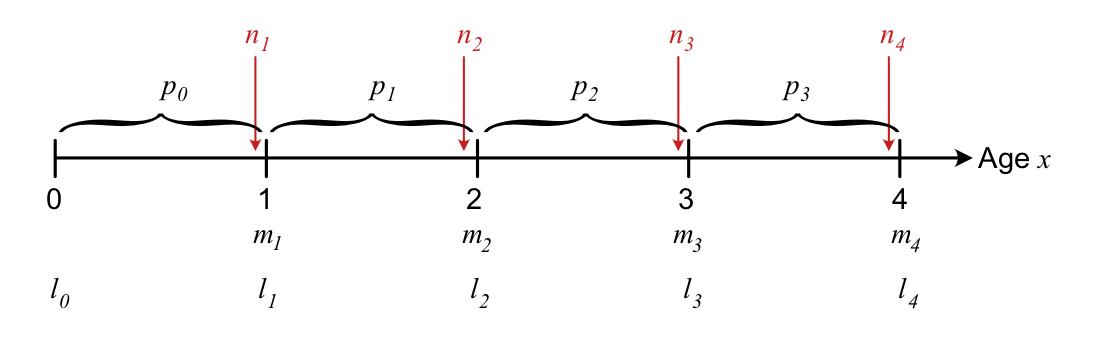
\includegraphics[width=1\linewidth]{SurvFecPreRep2} \caption{Overview of the timing of different events of survival and reproduction within each time step, for a pre-reproductive census.}\label{fig:fig3}
\end{figure}

With a \textbf{pre-reproductive census}, offspring will be nearly 1 year old when counted, and age classes correspond to the actual age at counting (e.g.~individuals in age class 1 are 1 year old when counted), so that \(s_j=p_j\). The fertility coefficients are then given by \(f_j=p_0m_j\), the product of the fecundity \(m_j\) and the first year survival probability \(p_0\).

\hypertarget{bird-example-4}{%
\subsubsection*{Bird example}\label{bird-example-4}}
\addcontentsline{toc}{subsubsection}{Bird example}

Using the bird example introduced in section \ref{bird}, the Leslie matrix for a pre-reproductive census is given by

\begin{align}
\begin{split}
\mathbf{A}=\left[\begin{matrix} f_1 & f_2 &f_3  \\ s_1 &0&0\\ 0 & s_2 &0  \\  \end{matrix}\right]=\left[\begin{matrix} 0 & p_0m_2 &p_0m_3  \\ p_1 &0&0\\ 0 & p_2 &0  \\  \end{matrix}\right]=\left[\begin{matrix} 0 &0.6 &1.2  \\ 0.9 &0&0\\ 0 & 0.6 &0  \\  \end{matrix}\right].
\end{split}
\label{eq:Prerep}
\end{align}

The classes of this matrix corresponds to age 1, 2, and 3. We do not `see' the 0-year olds in the matrix model, but the survival probability \(p_0\) enters the fertility coefficients.

In R, we can define the matrix as follows:

\begin{Shaded}
\begin{Highlighting}[]
\NormalTok{Abird.pre }\OtherTok{\textless{}{-}} \FunctionTok{Create.Amat}\NormalTok{(Svec }\OtherTok{\textless{}{-}} \FunctionTok{c}\NormalTok{(.}\DecValTok{9}\NormalTok{, .}\DecValTok{6}\NormalTok{, }\DecValTok{0}\NormalTok{), }\AttributeTok{Fvec=} \FunctionTok{c}\NormalTok{(}\DecValTok{0}\NormalTok{, .}\DecValTok{6}\NormalTok{, }\FloatTok{1.2}\NormalTok{))  }
\end{Highlighting}
\end{Shaded}

\hypertarget{post-reproductive-census}{%
\subsection{Post-reproductive census}\label{post-reproductive-census}}

\begin{figure}
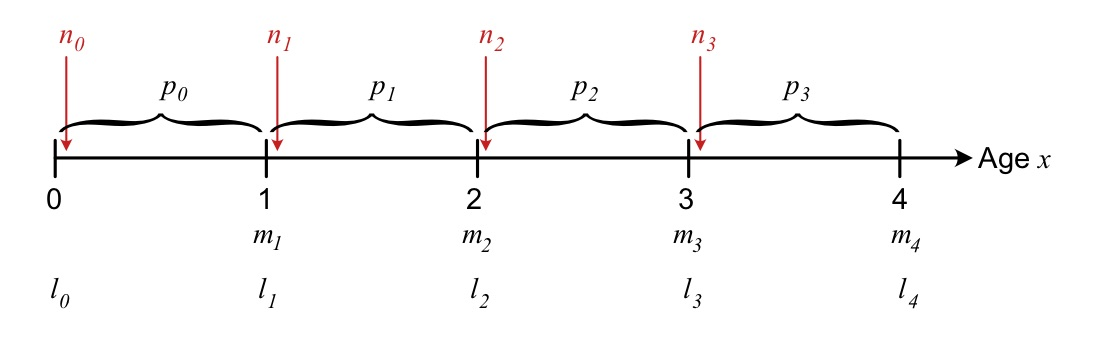
\includegraphics[width=1\linewidth]{SurvFecPostRep2} \caption{Overview of the timing of different events of survival and reproduction within each time step, for a post-reproductive census.}\label{fig:fig4}
\end{figure}

With a \textbf{post-reproductive census}, the population is counted right after reproduction. In this case, age class 1 consists of newborn individuals (age 0), and individuals in age class \(j\) have the actual age \(j-1\), so that \(s_j=p_{j-1}\). The fertility coefficient \(f_j\) now depends on survival of the parent from last time step \(s_{j-1}\), and on fecundity \(m_{j}\) of the age \(j\), since individuals reproduce right before next census. Thus, the fertility coefficient of the Leslie matrix is now \(f_j=p_{j-1}m_{j}\). This definition of fertilities can be counter-intuitive, as the contribution from a given age class \(j\) to next year's offspring depends on survival from the previous (actual) age \(p_{j-1}\).

\hypertarget{bird-example-5}{%
\subsubsection*{Bird example}\label{bird-example-5}}
\addcontentsline{toc}{subsubsection}{Bird example}

For the bird example, we get the following Leslie matrix with post-reproductive census:

\begin{align}
\begin{split}
\mathbf{A}=\left[\begin{matrix} f_1 & f_2 &f_3  \\ s_1 &0&0\\ 0 & s_2 &0  \\  \end{matrix}\right]=\left[\begin{matrix} 0 & p_1m_2 &p_2m_3  \\ p_0 &0&0\\ 0 & p_1 &0  \\  \end{matrix}\right]=\left[\begin{matrix} 0 &2.7 &3.6  \\ 0.2 &0&0\\ 0 & 0.9 &0  \\  \end{matrix}\right].
\end{split}
\label{eq:Postrep}
\end{align}

Note that each class of this matrix corresponds to age 0, 1, and 2. Thus, in this case we do not `see' the 3-year olds as a separate class, but their fecundity defines fertility coefficient in the third class.

In R, we can define this matrix as follows:

\begin{Shaded}
\begin{Highlighting}[]
\NormalTok{Abird.post }\OtherTok{\textless{}{-}} \FunctionTok{Create.Amat}\NormalTok{(Svec }\OtherTok{\textless{}{-}} \FunctionTok{c}\NormalTok{(.}\DecValTok{2}\NormalTok{, .}\DecValTok{9}\NormalTok{, }\DecValTok{0}\NormalTok{), }\AttributeTok{Fvec=} \FunctionTok{c}\NormalTok{(}\DecValTok{0}\NormalTok{, }\FloatTok{2.7}\NormalTok{, }\FloatTok{3.6}\NormalTok{))  }
\end{Highlighting}
\end{Shaded}

\hypertarget{avoiding-mistakes}{%
\subsection{Avoiding mistakes}\label{avoiding-mistakes}}

It turns out that mistakes in constructing the projection matrix are quite common in the ecological literature \citep{Kendall8}, and issues with census time often play a role here. Mistakes are easily made, since keeping track of age classes versus actual age requires accurate `book-keeping', especially with a post-reproductive census. Mistakes are also more common for post-reproductive census models than pre-reproductive census models \citep{Kendall8}.

Contributing to the confusion, the terminology of matrix models is not consistent in the literature. For instance, what we have defined as the `fertility coefficients' \(f_j\) is by some authors referred to as `fecundity' (\(m_j\) in our notation). Therefore, some authors mistakenly did not include survival in their fertility coefficients. Finally, there is no general consensus on whether to use 0 or 1 as index for the first age class when a post-reproductive census is used (note that we always use 1 as the index, regardless of census time), and this choice can affect the limits and indexing in different calculations (e.g.~the Euler-Lotka equation).

The main recommendation to avoid such errors when constructing a matrix model, is to take your time and make sure you have defined each element of the matrix model and its biological meaning. One way to double check that you have obtained the right coefficients is to compare a pre- and post-reproductive census model and Leslie matrix, and check that \(\lambda\) calculated from the matrix (section\ref{asymptotic}) is the same for the two cases. If it differs, at least one of the models has an error. It can also be helpful to draw a life cycle graph (see section \ref{life-cycle-graph}).

The long-term population growth rate \(\lambda\) should be the same regardless of census time, and for age structured models the same is true for \(R_0\) and generation time \(G\) (section\ref{asymptotic}). But other properties will change between census times, such as the stable stage structure and reproductive value. The difference can be large, since many changes can occur within time steps. This is particularly true for species producing a many offspring per reproductive event, with low offspring survival. A female cod, for instance, can produce millions of eggs, but only a few will survive the first year. If we count a cod population right after spawning (post-reproductive census), the fertilized eggs would constitute a very high proportion of the population (practically the entire population). If we instead counted the population right before spawning (pre-reproductive census), the proportion of age 1 offspring would not be as high.

\hypertarget{life-cycle-graph}{%
\section{Life cycle graph}\label{life-cycle-graph}}

\begin{figure}
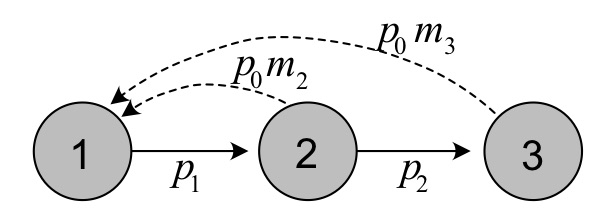
\includegraphics[width=0.6\linewidth]{LifeCycleAgePRE} \caption{Life cycle graph for the songbird example, with a pre-reproductive census.}\label{fig:Birdfig}
\end{figure}

A structured model can be represented in different ways. You have already seen two examples for age-structured populations: A life table and a matrix model. A third representation, which is a helpful visual tool, is the life cycle graph. This is particularly useful for more complex structures than age structure, with many possible transitions among stages. For age structured popualtoins it can be a useful tool to keep track of parameters for the different census times.

A life cycle graph gives an overview of the possible transitions among age classes each time step. For age structured populations, these transitions are quite simple, as they only consist of of survival from one age class to the next, and reproductive contributions from each age class to next year's offspring.

Figure \ref{fig:Birdfig} shows the life cycle graph for the bird example introduced in section \ref{bird}, for a pre-reproductive census. Each circle represent one age class of the matrix model, and since this is pre-reproductive census age class 1 consists of individuals at age 1, etc. The circles are connected by arrows representing survival and reproduction. Comparing the life cycle graph to the Leslie matrix described before (equation \eqref{eq:Prerep}), we see how the transitions are represented in the projection matrix.

\hypertarget{projected-growth}{%
\section{Projected growth}\label{projected-growth}}

The simplest application of a projection matrix is to use it to project the growth of each age class over time, from some given initial population vector \(\mathbf{n}_0\) to a desired number of time steps \(T_{max}\). The following R function performs such a projection for a given Leslie matrix \(\mathbf{A}\), and returns the number of individuals in each age class at each time step in a data frame.

\begin{Shaded}
\begin{Highlighting}[]
\NormalTok{projection }\OtherTok{\textless{}{-}} \ControlFlowTok{function}\NormalTok{(MatA, }\AttributeTok{Tmax =} \DecValTok{50}\NormalTok{, n0)\{}
\NormalTok{  k }\OtherTok{\textless{}{-}} \FunctionTok{dim}\NormalTok{(MatA)[}\DecValTok{1}\NormalTok{]}
  \ControlFlowTok{if}\NormalTok{(}\FunctionTok{length}\NormalTok{(n0)}\SpecialCharTok{!=}\NormalTok{k)\{}
      \FunctionTok{warning}\NormalTok{(}\StringTok{"n0 should have length k corresponding to number of stages in Amat"}\NormalTok{)}
\NormalTok{      \}}
\NormalTok{  Nmat }\OtherTok{\textless{}{-}} \FunctionTok{matrix}\NormalTok{(}\ConstantTok{NA}\NormalTok{, }\AttributeTok{nrow=}\NormalTok{ Tmax}\SpecialCharTok{+}\DecValTok{1}\NormalTok{, }\AttributeTok{ncol=}\NormalTok{k)}
\NormalTok{  cnames }\OtherTok{\textless{}{-}} \FunctionTok{paste}\NormalTok{(}\StringTok{"n"}\NormalTok{, }\DecValTok{1}\SpecialCharTok{:}\NormalTok{k, }\AttributeTok{sep=}\StringTok{""}\NormalTok{)}
\NormalTok{  timesteps }\OtherTok{\textless{}{-}} \DecValTok{0}\SpecialCharTok{:}\NormalTok{Tmax}
\NormalTok{  Nmat[}\DecValTok{1}\NormalTok{,] }\OtherTok{=}\NormalTok{ n0 }
  \ControlFlowTok{for}\NormalTok{(i }\ControlFlowTok{in} \DecValTok{2}\SpecialCharTok{:}\NormalTok{(Tmax}\SpecialCharTok{+}\DecValTok{1}\NormalTok{))\{  }
\NormalTok{    Nmat[i,] }\OtherTok{=}\NormalTok{ MatA}\SpecialCharTok{\%*\%}\NormalTok{Nmat[i}\DecValTok{{-}1}\NormalTok{,]}
\NormalTok{  \}}
\NormalTok{  frame }\OtherTok{\textless{}{-}} \FunctionTok{data.frame}\NormalTok{(timesteps, Nmat)}
  \FunctionTok{colnames}\NormalTok{(frame) }\OtherTok{\textless{}{-}} \FunctionTok{c}\NormalTok{(}\StringTok{"time"}\NormalTok{, cnames)}
\NormalTok{  frame}
\NormalTok{\}}
\end{Highlighting}
\end{Shaded}

In R, the operator \(\%*\%\) performs a matrix multiplication. Here this is done for each time step within a for-loop to calculate the current population vector as a function of the previous one. Note that the initial population vector \(n_0\) has to have correct number of element \(k\), i.e.~the same number of age classes as in the projection matrix \(\mathbf{A}\). If not you will get an error when using the function. The initial population vector is included the returned data frame (the first row).

\hypertarget{bird-example-6}{%
\subsubsection*{Bird example}\label{bird-example-6}}
\addcontentsline{toc}{subsubsection}{Bird example}

For the bird example (section \ref{bird}), we can apply the function to project the population over time. The projection matrices for a pre- or post-reproductive census were defined earlier for this example. We can use the following code to project and plot the population over time for each census type:

\begin{Shaded}
\begin{Highlighting}[]
\CommentTok{\#Return matrix of projected growth of each age class over time:}
\NormalTok{Pop.bird.pre }\OtherTok{\textless{}{-}} \FunctionTok{projection}\NormalTok{(}\AttributeTok{MatA=}\NormalTok{Abird.pre, }\AttributeTok{n0=}\FunctionTok{rep}\NormalTok{(}\DecValTok{10}\NormalTok{,}\DecValTok{3}\NormalTok{), }\AttributeTok{Tmax=}\DecValTok{30}\NormalTok{)}
\NormalTok{Pop.bird.post }\OtherTok{\textless{}{-}} \FunctionTok{projection}\NormalTok{(}\AttributeTok{MatA=}\NormalTok{Abird.post, }\AttributeTok{n0=}\FunctionTok{rep}\NormalTok{(}\DecValTok{10}\NormalTok{,}\DecValTok{3}\NormalTok{),}\AttributeTok{Tmax=}\DecValTok{30}\NormalTok{)}

\CommentTok{\#Long format for plotting:}
\NormalTok{Pop.bird.pre.long }\OtherTok{\textless{}{-}}\NormalTok{ Pop.bird.pre }\SpecialCharTok{\%\textgreater{}\%} \FunctionTok{pivot\_longer}\NormalTok{(}\FunctionTok{c}\NormalTok{(}\SpecialCharTok{{-}}\NormalTok{time),}
               \AttributeTok{names\_to =} \StringTok{"AgeClass"}\NormalTok{, }\AttributeTok{values\_to =} \StringTok{"Value"}\NormalTok{)}
\NormalTok{Pop.bird.post.long }\OtherTok{\textless{}{-}}\NormalTok{ Pop.bird.post }\SpecialCharTok{\%\textgreater{}\%} \FunctionTok{pivot\_longer}\NormalTok{(}\FunctionTok{c}\NormalTok{(}\SpecialCharTok{{-}}\NormalTok{time),}
               \AttributeTok{names\_to =} \StringTok{"AgeClass"}\NormalTok{, }\AttributeTok{values\_to =} \StringTok{"Value"}\NormalTok{)}

\CommentTok{\#Add census type and combine:}
\NormalTok{Pop.bird.pre.long}\SpecialCharTok{$}\NormalTok{census }\OtherTok{\textless{}{-}} \StringTok{"Pre"} 
\NormalTok{Pop.bird.post.long}\SpecialCharTok{$}\NormalTok{census }\OtherTok{\textless{}{-}} \StringTok{"Post"} 
\NormalTok{Pop.bird.long }\OtherTok{\textless{}{-}} \FunctionTok{rbind}\NormalTok{(Pop.bird.pre.long,Pop.bird.post.long)}

\CommentTok{\#Order levels of the census factor variables}
\NormalTok{Pop.bird.long}\SpecialCharTok{$}\NormalTok{census }\OtherTok{\textless{}{-}} \FunctionTok{factor}\NormalTok{(Pop.bird.long}\SpecialCharTok{$}\NormalTok{census, }\AttributeTok{levels=}\FunctionTok{c}\NormalTok{(}\StringTok{"Pre"}\NormalTok{,}\StringTok{"Post"}\NormalTok{))}

\CommentTok{\#Plot}

\FunctionTok{ggplot}\NormalTok{(Pop.bird.long) }\SpecialCharTok{+} 
  \FunctionTok{geom\_line}\NormalTok{(}\FunctionTok{aes}\NormalTok{(}\AttributeTok{x=}\NormalTok{time,}\AttributeTok{y=}\NormalTok{Value, }\AttributeTok{col=}\NormalTok{AgeClass, }\AttributeTok{linetype=}\NormalTok{AgeClass), }\AttributeTok{lwd=}\FloatTok{1.2}\NormalTok{)}\SpecialCharTok{+}
  \FunctionTok{theme\_bw}\NormalTok{() }\SpecialCharTok{+}
  \FunctionTok{facet\_wrap}\NormalTok{(}\FunctionTok{vars}\NormalTok{(census),}\AttributeTok{ncol=}\DecValTok{2}\NormalTok{)}\SpecialCharTok{+}
  \FunctionTok{scale\_color\_manual}\NormalTok{(}\AttributeTok{values=}\NormalTok{colors3)}\SpecialCharTok{+} \CommentTok{\#Add colors manually}
  \FunctionTok{scale\_linetype\_manual}\NormalTok{(}\AttributeTok{values=}\FunctionTok{c}\NormalTok{(}\DecValTok{1}\NormalTok{,}\DecValTok{2}\NormalTok{,}\DecValTok{3}\NormalTok{))}\SpecialCharTok{+} \CommentTok{\#Add linetypes manually}
  \FunctionTok{labs}\NormalTok{( }\AttributeTok{x=}\StringTok{"Time (year)"}\NormalTok{, }\AttributeTok{y=}\StringTok{"Age class size"}\NormalTok{)}\SpecialCharTok{+} \CommentTok{\#Axis labels}
  \FunctionTok{theme}\NormalTok{(}\AttributeTok{legend.position =} \StringTok{"top"}\NormalTok{ ) }\CommentTok{\#Place legend on top}
\end{Highlighting}
\end{Shaded}

\begin{figure}
\centering
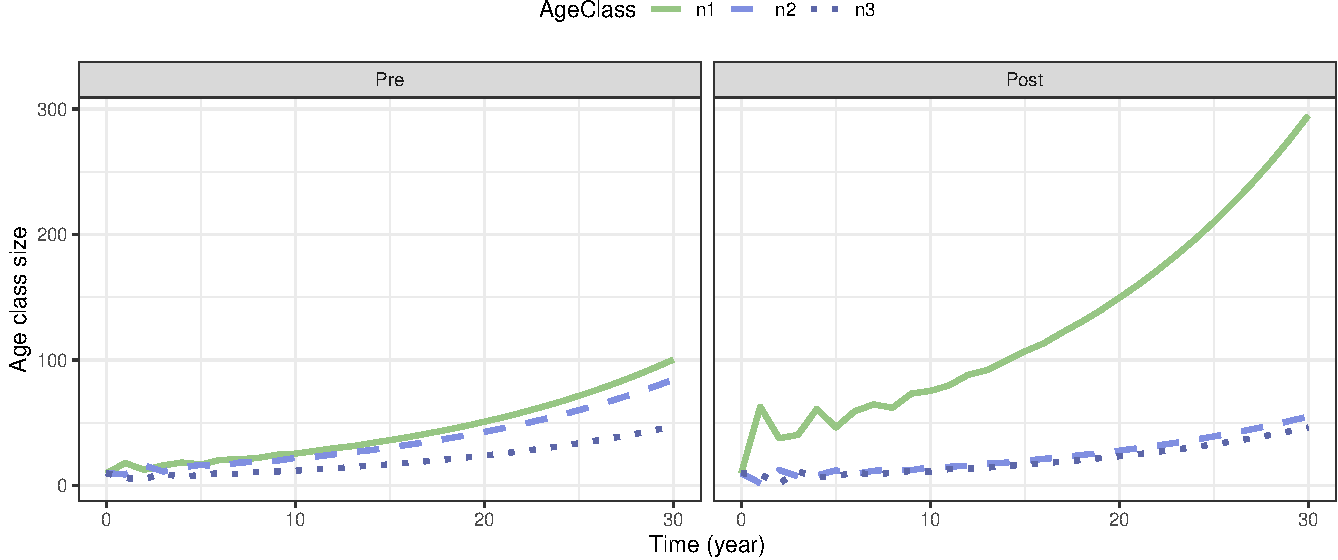
\includegraphics{DemographyCompendium_files/figure-latex/birdgrowth-1.pdf}
\caption{\label{fig:birdgrowth}Projected growth of the bird example, with pre-reproductive (age class 1 consist of 1-year olds) or post-reproductive census (age class 1 consist of 0-year olds).}
\end{figure}

Figure \ref{fig:birdgrowth} shows the difference between the pre-reproductive an post-reproductive census in the bird example. With pre-reproductive census the first age class consists of 1-year olds, the second class of 2-year olds and the third class of 3-year olds. With post-reproductive census the first class consists of individuals of age 0, the second of age 1 and the third of age 2. In each model we start with 10 individuals in each class, but the subsequent growth pattern is different because of how the population is counted. We see a higher number of individuals in the first class of the post reproductive census model compared to the other classes, due to high reproduction in this example.

Note the fluctuations in the beginning, that become smoother over time and eventually disappear. These occur because the population is started with 10 individuals in each class, which is not the stable structure of the population. The fluctuatoins are called \textbf{transient fluctuations} because they are temporary. After some time they become negligible, as the population reachedes a phase of \textbf{stable growth}, where each age class grows exponentially with the same rate \(\lambda\). In this phase the population shows \textbf{asymptotic dynamics}, and it will remain there unless something disturbs the stable structure. There are three properties of the population in the asymptotic phase: The long-term growth rate \(\lambda\), the stable age structure \(\mathbf{u}\), and the reproductive values \(\mathbf{v}\). The next section describes how to calculate these properties from the projected growth, while section \ref{asymptotic} shows how to calculate these properties from the projection matrix and its two main components. Here the different properties and their biological meaning are discussed in more detail.

\hypertarget{asymptotic}{%
\section{Asymptotic properties}\label{asymptotic}}

\hypertarget{projected}{%
\subsection{Calculations based on projected growth}\label{projected}}

From the population projections we can now estimate \(\lambda\), the stable age structure \(\mathbf{u}\), and the reproductive values \(\mathbf{v}\), as shown in the next sections.

\hypertarget{long-term-population-growth-rate-lambda}{%
\subsubsection*{\texorpdfstring{Long-term population growth rate \(\lambda\):}{Long-term population growth rate \textbackslash lambda:}}\label{long-term-population-growth-rate-lambda}}
\addcontentsline{toc}{subsubsection}{Long-term population growth rate \(\lambda\):}

This is the same growth rate \(\lambda\) that we have already defined based on the Euler-Lotka equation (section \ref{Euler}). This parameter can also be estimated from the projected population size over time, as \(\lambda=N_{T+1}/N_T\) (where \(N_t=\sum_{i=1}^kn_{i,t}\) is the total population size at time \(t\)), after a sufficiently large number of time steps \(T\) (large enough that the estimate of \(\lambda\), to a chosen number of decimal places, does not change if we increase \(T\) further). It can also be estimated from any of the age classes,

For the bird example (here with prereproductive census), we can use the following R code:

\begin{Shaded}
\begin{Highlighting}[]
\NormalTok{Total.pop.bird }\OtherTok{\textless{}{-}} \FunctionTok{apply}\NormalTok{(Pop.bird.pre[}\SpecialCharTok{{-}}\DecValTok{1}\NormalTok{],}\DecValTok{1}\NormalTok{,sum) }\CommentTok{\#Get total population size}
\NormalTok{Tmax }\OtherTok{\textless{}{-}} \FunctionTok{length}\NormalTok{(Total.pop.bird)}\CommentTok{\#Recover max time}
\NormalTok{lambda.bird }\OtherTok{\textless{}{-}}\NormalTok{ Total.pop.bird[Tmax]}\SpecialCharTok{/}\NormalTok{Total.pop.bird[Tmax}\DecValTok{{-}1}\NormalTok{]}
\end{Highlighting}
\end{Shaded}

The estimated value from projection over 31 time steps is \(\lambda\approx\) 1.07027, close to the value \$\lambda\approx\$1.07025 calculated from the life table in section \ref{Euler}. The more time steps are used for the projection and calculation, the more accurate the estimate of \(\lambda\) will be.

\hypertarget{stable-age-structure}{%
\subsubsection*{Stable age structure:}\label{stable-age-structure}}
\addcontentsline{toc}{subsubsection}{Stable age structure:}

The age structure is the proportion of the population constituted by each age class. As you can see from the projected growth (figure \ref{fig:birdgrowth}), the age structure will fluctuate in the beginning, before it approaches a \textbf{stable age structure} as the transient fluctuations fade out, a structure that becomes constant over time. The stable age structure is denoted by the vector \(\mathbf{u}=[u_1, u_2, ..., u_k]\) (where \(\sum_{j=1}^{k} u_j=1\)). This vector can be estimated from the projected population, as \(u_j\approx n_{j,T}/N_T\), where again \(T\) is a (sufficiently) large number of time steps. For growing age structured populations, the age structure will always be a monotonically decreasing function of age class.

In R, we can also estimate the stable structure from the projections, here shown for the bird example with pre-reproductive census:

\begin{Shaded}
\begin{Highlighting}[]
\NormalTok{stablestructure.pre }\OtherTok{\textless{}{-}}\NormalTok{ Pop.bird.pre[Tmax,}\SpecialCharTok{{-}}\DecValTok{1}\NormalTok{]}\SpecialCharTok{/}\NormalTok{Total.pop.bird[Tmax]}

\NormalTok{k }\OtherTok{\textless{}{-}} \FunctionTok{dim}\NormalTok{(Abird.pre)[}\DecValTok{1}\NormalTok{]}

\FunctionTok{names}\NormalTok{(stablestructure.pre) }\OtherTok{\textless{}{-}} \FunctionTok{paste}\NormalTok{(}\StringTok{"u"}\NormalTok{,}\DecValTok{1}\SpecialCharTok{:}\NormalTok{k,}\AttributeTok{sep=}\StringTok{""}\NormalTok{)}

\NormalTok{stablestructure.pre}
\end{Highlighting}
\end{Shaded}

\begin{verbatim}
##           u1        u2        u3
## 31 0.4324629 0.3636527 0.2038843
\end{verbatim}

\hypertarget{reproductive-values}{%
\subsubsection*{Reproductive values:}\label{reproductive-values}}
\addcontentsline{toc}{subsubsection}{Reproductive values:}

We can calculate the age-specific \textbf{reproductive values} using a slightly modified version of projected growth. The reproductive value was first defined by \citet{Fisher1}, who was interested in how much individuals of each age class would contribute to the future population, compared to other age classes. We can think of the reproductive value as a return rate associated with `investing' in different age classes. If we could choose individuals from just one age class to start a new population, and wanted this population to be as large as possible after some time - we should choose the age class with the highest reproductive value.

To calculate the reproductive values from projections, we have two options: One is to project the total population size \(k\) times (where \(k\) the number of age classes), and at projection number \(i\) we start with a given number of individuals (e.g.~10) in age class \(i\) only (and zero in the other classes). The relative differences between the projected population sizes after \(T\) time steps then reflect the reproductive values. The vector \(\mathbf{v}\) (a row vector) can be scaled in different ways, here we will use the scaling \(\mathbf{vu}=\sum_{j=1}^kv_ju_j=1\).

Another approach is to use the \emph{transposed} Leslie matrix \(\mathbf{A}^T\) (taking the transpose means `flipping' the matrix over the main diagonal, so that rows and columns are switched) and do the same kind of projection as for the stable age structure before applying the scaling defined above.

We can use the following code to apply the second approach for the bird example (pre-reproductive model):

\begin{Shaded}
\begin{Highlighting}[]
\NormalTok{Pop.bird.transpose }\OtherTok{\textless{}{-}} \FunctionTok{projection}\NormalTok{(}\AttributeTok{MatA=}\FunctionTok{t}\NormalTok{(Abird.pre), }\AttributeTok{n0=}\FunctionTok{rep}\NormalTok{(}\DecValTok{10}\NormalTok{,}\DecValTok{3}\NormalTok{)) }\CommentTok{\#Projected growth using the transpose Leslie matrix.}

\NormalTok{k }\OtherTok{\textless{}{-}} \FunctionTok{dim}\NormalTok{(Abird.pre)[}\DecValTok{1}\NormalTok{]}

\NormalTok{repvalues.pre }\OtherTok{\textless{}{-}}\NormalTok{ Pop.bird.transpose[Tmax,}\SpecialCharTok{{-}}\DecValTok{1}\NormalTok{]}\SpecialCharTok{/}\FunctionTok{sum}\NormalTok{(stablestructure.pre}\SpecialCharTok{*}\NormalTok{Pop.bird.transpose[Tmax,}\SpecialCharTok{{-}}\DecValTok{1}\NormalTok{])}
\FunctionTok{names}\NormalTok{(repvalues.pre) }\OtherTok{\textless{}{-}} \FunctionTok{paste}\NormalTok{(}\StringTok{"v"}\NormalTok{,}\DecValTok{1}\SpecialCharTok{:}\NormalTok{k,}\AttributeTok{sep=}\StringTok{""}\NormalTok{)}

\NormalTok{repvalues.pre}
\end{Highlighting}
\end{Shaded}

\begin{verbatim}
##           v1       v2       v3
## 31 0.9144873 1.087482 1.025347
\end{verbatim}

Note that the reproductive value of an age class is a relative measure (the value should always be interpreted in comparison to the other classes). If some environmental change alters the survival and fecundity in one age class, this will generally affect the reproductive value not only in this class, but in all the other age classes as well.

\hypertarget{eigen}{%
\subsection{Calculations based on projection matrix}\label{eigen}}

You have now seen how the Leslie matrix \(\mathbf{A}\) (or its transpose) can be used to project the population over time, and how we could calculate \(\lambda\), \(\mathbf{u}\) and \(\mathbf{v}\) based on these projections. This method of estimation is intuitive and works well for a given model, such as our bird example, but it takes some time and is not the most efficient way to calculate these properties. A much more efficient way is to calculate these properties directly from the projection matrix \(\mathbf{A}\), using the eigenvalues and eigenvectors (socalled `eigen analysis'.

The mathematical details of these calculations are outside the scope of this introduction (see e.g. \citet{Caswell1} for a more detailed introduction), but they are routinely included in R packages and easily defined in custom functions as well (as we will do below). In short, given that certain properties of \(\mathbf{A}\) are fulfilled (which they are for most biologically relevant matrix models), \(\lambda\) is the dominant eigenvalue of \(\mathbf{A}\), \(\mathbf{u}\) is the right eigenvector associated with \(\lambda\), and \(\mathbf{v}\) is the left eigenvector. It is worth noting that for age-structured populations, the socalled \emph{characteristic equation} of the matrix \(\mathbf{A}\), from which we all of these parameters are calculated, corresponds to the Euler-Lotka equation we defined in section \ref{Euler}.

The following R function takes a Leslie matrix (or any other kind of projection matrix) as the input variable, and returns the value of \(\lambda\) along with the vectors \(\mathbf{u}\) and \(\mathbf{v}\), using the scaling defined above.

\begin{Shaded}
\begin{Highlighting}[]
\NormalTok{uvlambda }\OtherTok{\textless{}{-}} \ControlFlowTok{function}\NormalTok{(MatA)\{}
\NormalTok{ ev }\OtherTok{\textless{}{-}} \FunctionTok{eigen}\NormalTok{(MatA)}
\NormalTok{ tev }\OtherTok{\textless{}{-}} \FunctionTok{eigen}\NormalTok{(}\FunctionTok{t}\NormalTok{(MatA))}
\NormalTok{ lmax }\OtherTok{\textless{}{-}} \FunctionTok{which.max}\NormalTok{(}\FunctionTok{Re}\NormalTok{(ev}\SpecialCharTok{$}\NormalTok{values))}
\NormalTok{ U }\OtherTok{\textless{}{-}}\NormalTok{ ev}\SpecialCharTok{$}\NormalTok{vectors}
\NormalTok{ V }\OtherTok{\textless{}{-}}\NormalTok{ tev}\SpecialCharTok{$}\NormalTok{vectors}
\NormalTok{ u }\OtherTok{\textless{}{-}} \FunctionTok{as.matrix}\NormalTok{(}\FunctionTok{abs}\NormalTok{(}\FunctionTok{Re}\NormalTok{(U[, lmax]))}\SpecialCharTok{/}\FunctionTok{sum}\NormalTok{(}\FunctionTok{abs}\NormalTok{(}\FunctionTok{Re}\NormalTok{(U[, lmax]))))}
\NormalTok{ u }\OtherTok{\textless{}{-}}\NormalTok{ u}\SpecialCharTok{/}\NormalTok{(}\FunctionTok{sum}\NormalTok{(u)) }\CommentTok{\#scale u}
\NormalTok{ v }\OtherTok{\textless{}{-}} \FunctionTok{as.matrix}\NormalTok{(}\FunctionTok{abs}\NormalTok{(}\FunctionTok{Re}\NormalTok{(V[, lmax])))}
\NormalTok{ v }\OtherTok{\textless{}{-}}\NormalTok{ v}\SpecialCharTok{/}\FunctionTok{sum}\NormalTok{(u}\SpecialCharTok{*}\NormalTok{v ) }\CommentTok{\#scale v}
\NormalTok{ v }\OtherTok{\textless{}{-}} \FunctionTok{t}\NormalTok{(}\FunctionTok{ifelse}\NormalTok{(u}\SpecialCharTok{*}\NormalTok{v }\SpecialCharTok{\textless{}=} \DecValTok{0}\NormalTok{, }\DecValTok{0}\NormalTok{, v))}
 \FunctionTok{return}\NormalTok{(}\FunctionTok{list}\NormalTok{(}\StringTok{"lambda"}\OtherTok{=}\FunctionTok{max}\NormalTok{(}\FunctionTok{Re}\NormalTok{(ev}\SpecialCharTok{$}\NormalTok{values)),}\StringTok{"u"}\OtherTok{=}\NormalTok{u,}\StringTok{"v"}\OtherTok{=}\NormalTok{v))}
\NormalTok{\}}
\end{Highlighting}
\end{Shaded}

\hypertarget{bird-example-7}{%
\subsubsection*{Bird example}\label{bird-example-7}}
\addcontentsline{toc}{subsubsection}{Bird example}

For the bird example with a pre-reproductive census, we can calculate and plot the asymptotic properties as follows:

\begin{Shaded}
\begin{Highlighting}[]
\NormalTok{res.bird }\OtherTok{\textless{}{-}} \FunctionTok{uvlambda}\NormalTok{(Abird.pre)}
\NormalTok{lambda.bird.pre }\OtherTok{\textless{}{-}}\NormalTok{ res.bird}\SpecialCharTok{$}\NormalTok{lambda}
\NormalTok{u.bird.pre }\OtherTok{\textless{}{-}}\NormalTok{ res.bird}\SpecialCharTok{$}\NormalTok{u}
\NormalTok{v.bird.bird }\OtherTok{\textless{}{-}}\NormalTok{ res.bird}\SpecialCharTok{$}\NormalTok{v}

\CommentTok{\#Create data frame for plotting}
\NormalTok{birdframe.asym }\OtherTok{\textless{}{-}} \FunctionTok{data.frame}\NormalTok{(}\StringTok{"AgeClass"}\OtherTok{=}\DecValTok{1}\SpecialCharTok{:}\DecValTok{3}\NormalTok{, }\StringTok{"u"}\OtherTok{=}\NormalTok{u.bird.pre, }\StringTok{"v"}\OtherTok{=}\FunctionTok{t}\NormalTok{(v.bird.bird))}

\CommentTok{\#Long format for plotting:}
\NormalTok{birdframe.asym.long }\OtherTok{\textless{}{-}}\NormalTok{ birdframe.asym }\SpecialCharTok{\%\textgreater{}\%} \FunctionTok{pivot\_longer}\NormalTok{(}\FunctionTok{c}\NormalTok{(u,v),}
               \AttributeTok{names\_to =} \StringTok{"Vector"}\NormalTok{, }\AttributeTok{values\_to =} \StringTok{"Value"}\NormalTok{)}

\CommentTok{\#Ensure order of factor levels (for plotting)}
\NormalTok{birdframe.asym.long}\SpecialCharTok{$}\NormalTok{AgeClass}\OtherTok{\textless{}{-}} \FunctionTok{factor}\NormalTok{(birdframe.asym.long}\SpecialCharTok{$}\NormalTok{AgeClass, }\AttributeTok{levels=}\FunctionTok{c}\NormalTok{(}\DecValTok{1}\NormalTok{,}\DecValTok{2}\NormalTok{,}\DecValTok{3}\NormalTok{))}

\FunctionTok{ggplot}\NormalTok{(birdframe.asym.long) }\SpecialCharTok{+} 
  \FunctionTok{geom\_col}\NormalTok{(}\FunctionTok{aes}\NormalTok{(}\AttributeTok{x=}\NormalTok{AgeClass, }\AttributeTok{y=}\NormalTok{Value, }\AttributeTok{fill=}\NormalTok{AgeClass ), }\AttributeTok{lwd=}\FloatTok{1.2}\NormalTok{)}\SpecialCharTok{+}
  \FunctionTok{theme\_bw}\NormalTok{() }\SpecialCharTok{+}
  \FunctionTok{facet\_wrap}\NormalTok{(}\FunctionTok{vars}\NormalTok{(Vector), }\AttributeTok{ncol=}\DecValTok{2}\NormalTok{, }\AttributeTok{scales=}\StringTok{"free"}\NormalTok{)}\SpecialCharTok{+}
  \FunctionTok{scale\_fill\_manual}\NormalTok{(}\AttributeTok{values=}\NormalTok{colors3)}\SpecialCharTok{+} \CommentTok{\#Add colors manually}
  \FunctionTok{labs}\NormalTok{( }\AttributeTok{x=}\StringTok{"Age class"}\NormalTok{, }\AttributeTok{y=}\StringTok{"Value"}\NormalTok{)}\SpecialCharTok{+} \CommentTok{\#Axis labels}
  \FunctionTok{theme}\NormalTok{(}\AttributeTok{legend.position =} \StringTok{"top"}\NormalTok{ ) }\CommentTok{\#Place legend on top}
\end{Highlighting}
\end{Shaded}

\begin{figure}
\centering
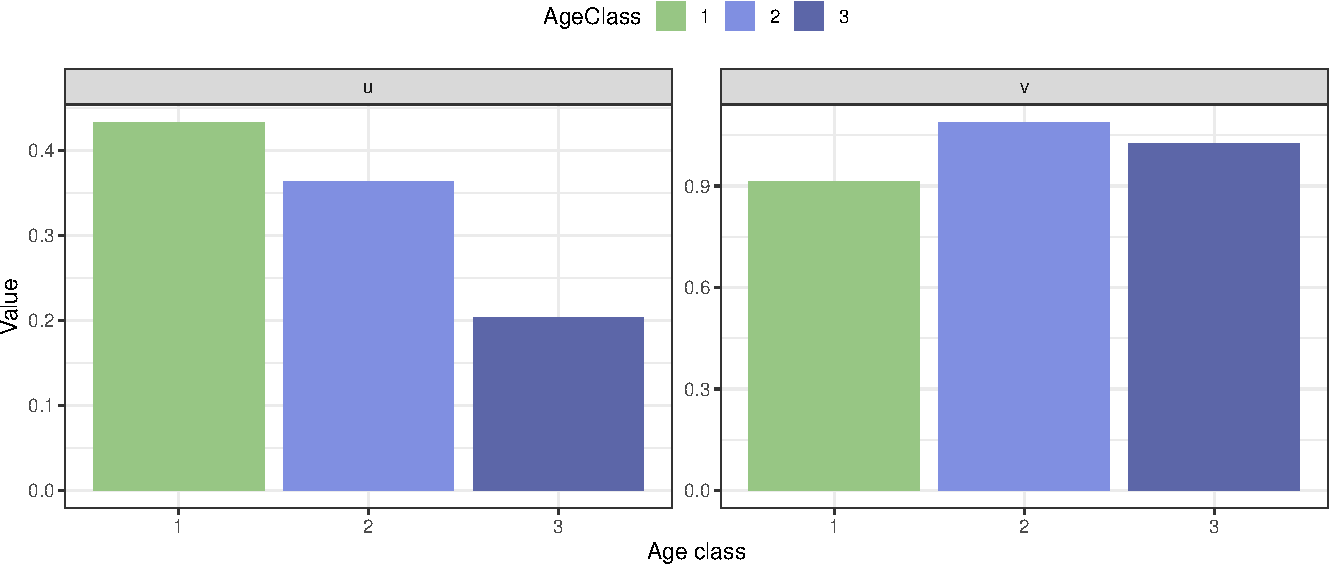
\includegraphics{DemographyCompendium_files/figure-latex/stablerepro-1.pdf}
\caption{\label{fig:stablerepro}Stable age structure and reproductive values, calculated for the bird example with pre-reproductive census.}
\end{figure}

The calculated long-term growth rate is \(\lambda=\) 1.0703 , corresponding well to the earlier result \(\lambda=\) 1.0703 calculated using projection.

Now we can also double check that we get the same value of \(\lambda\) for the pre-reproductive and post-reproductive bird models:

\begin{Shaded}
\begin{Highlighting}[]
\NormalTok{lambda.bird.pre }\OtherTok{\textless{}{-}} \FunctionTok{uvlambda}\NormalTok{(Abird.pre)}\SpecialCharTok{$}\NormalTok{lambda}
\NormalTok{lambda.bird.post }\OtherTok{\textless{}{-}} \FunctionTok{uvlambda}\NormalTok{(Abird.post)}\SpecialCharTok{$}\NormalTok{lambda}
\NormalTok{lambdas }\OtherTok{\textless{}{-}} \FunctionTok{c}\NormalTok{( lambda.bird.pre, lambda.bird.post)}
\FunctionTok{names}\NormalTok{(lambdas) }\OtherTok{\textless{}{-}} \FunctionTok{c}\NormalTok{(}\StringTok{"Pre"}\NormalTok{, }\StringTok{"Post"}\NormalTok{)}
\NormalTok{lambdas}
\end{Highlighting}
\end{Shaded}

\begin{verbatim}
##      Pre     Post 
## 1.070261 1.070261
\end{verbatim}

\hypertarget{lifetime}{%
\subsection{Life expectancy}\label{lifetime}}

From the matrix \(\mathbf{U}\) we can calculate the socalled fundamental matrix, from which we can find the life expectancy of each age class:

\begin{align}
\mathbf{N}=(\mathbf{I}-\mathbf{U})^{-1},
\label{eq:Fundamental}
\end{align}
where \(\mathbf{I}\) is an identity matrix (a matrix with 1's on the main diagonal and 0's everywhere else) of the same dimension as \(\mathbf{F}\) and \(\mathbf{U}\).

The column sums of this matrix provides the life expectancy (expected remaining lifetime) in each age class. The life expectancy at birth is given by the first element of the vector, if we assume a post-reproductive census model.

To calculate the vector of age class-specific life expectancies in R we can use the following function:

\begin{Shaded}
\begin{Highlighting}[]
\NormalTok{ LifeExpectancy }\OtherTok{\textless{}{-}} \ControlFlowTok{function}\NormalTok{(MatU)\{   }
\NormalTok{  k}\OtherTok{\textless{}{-}}\FunctionTok{dim}\NormalTok{(MatU)[}\DecValTok{1}\NormalTok{]}
  \ControlFlowTok{if}\NormalTok{(}\FunctionTok{is.na}\NormalTok{(MatU[k,k]))\{}
\NormalTok{    MatU[k,k]}\OtherTok{\textless{}{-}}\DecValTok{0}
\NormalTok{  \}}
\NormalTok{  uDim}\OtherTok{=}\FunctionTok{dim}\NormalTok{(MatU)[}\DecValTok{1}\NormalTok{]}
\NormalTok{  N }\OtherTok{=} \FunctionTok{solve}\NormalTok{(}\FunctionTok{diag}\NormalTok{(uDim[}\DecValTok{1}\NormalTok{])}\SpecialCharTok{{-}}\NormalTok{MatU)   }
  \FunctionTok{colSums}\NormalTok{(N)  }
\NormalTok{\}}
\end{Highlighting}
\end{Shaded}

\hypertarget{bird-example-8}{%
\subsubsection*{Bird example}\label{bird-example-8}}
\addcontentsline{toc}{subsubsection}{Bird example}

Using the post-reproductive model for the bird as an example, we get the following life expectancies:

\begin{Shaded}
\begin{Highlighting}[]
\CommentTok{\#Define MatU for the post{-}reproductive model:}
\NormalTok{Ubird.post }\OtherTok{\textless{}{-}}\NormalTok{ Abird.post}
\NormalTok{Ubird.post[}\DecValTok{1}\NormalTok{,] }\OtherTok{\textless{}{-}} \DecValTok{0} 

\CommentTok{\#Calculate life expectancy vector}
\NormalTok{ LifeExpectancy.bird.post }\OtherTok{\textless{}{-}} \FunctionTok{LifeExpectancy}\NormalTok{(}\AttributeTok{MatU=}\NormalTok{Ubird.post)}
\end{Highlighting}
\end{Shaded}

For the bird example (post-reproductive census), the age-specific life expectancy is {[}1.38, 1.9, 1{]} years. Note that the life expectancy in age class 2 (actual age 1) is higher than in age class 1 (age 0). This is because many individuals die during their first year. The life expectancy in age class 3 (age 2) is exactly one year, because all individuals die at age 3 (after reproducing).

\hypertarget{netrate}{%
\subsection{Lifetime reproduction}\label{netrate}}

Using the submatrices \(\mathbf{U}\) (survival matrix) and \(\mathbf{F}\) (fertility matrix), we can calculate the net reproductive rate \(R_0\) (mean lifetime reproduction), as well as the expected remaining reproduction of each class.

These calculations depend on the `generation to generation projection matrix'

\begin{align}
\mathbf{R}=\mathbf{F}(\mathbf{I}-\mathbf{U})^{-1}=\mathbf{F}\mathbf{N} 
\label{eq:RMatrix}
\end{align}
Note that the fundamental matrix (equation \ref(eq:Fundamental)) is also included in this definition. The matrix \(\mathbf{R}\) describes the generation to generation growth of each age class. The column sums of \(\mathbf{R}\) represent the expected remaining lifetime reproduction of the age class (with age structure, only the first row elements will be non-zero - but in more general stage structured models with more than one type of offspring, the matrix becomes more complex). \(R_0\) is the dominant eigenvalue of the matrix \(\mathbf{R}\), just like \(\lambda\) is the dominant eigenvalue of \(\mathbf{A}\) (remember that \(R_0\) is the population growth rate per generation).

In R, we can use the following function to calculate \(R_0\) and the column sums of the fundamental matrix, given the survival matrix \(\mathbf{U}\) and the fertility matrix \(\mathbf{F}\).

\begin{Shaded}
\begin{Highlighting}[]
\NormalTok{R0function  }\OtherTok{\textless{}{-}}  \ControlFlowTok{function}\NormalTok{(MatU, MatF)\{}
\NormalTok{  k }\OtherTok{\textless{}{-}} \FunctionTok{dim}\NormalTok{(MatU)[[}\DecValTok{1}\NormalTok{]]}
\NormalTok{  Rmat }\OtherTok{\textless{}{-}}\NormalTok{ MatF}\SpecialCharTok{\%*\%}\FunctionTok{solve}\NormalTok{(}\FunctionTok{diag}\NormalTok{(}\DecValTok{1}\NormalTok{, k, k)}\SpecialCharTok{{-}}\NormalTok{MatU)    }
\NormalTok{  Rvec }\OtherTok{\textless{}{-}} \FunctionTok{apply}\NormalTok{(Rmat,}\DecValTok{2}\NormalTok{,sum)}
\NormalTok{  R0 }\OtherTok{\textless{}{-}} \FunctionTok{uvlambda}\NormalTok{(}\AttributeTok{MatA=}\NormalTok{Rmat)}\SpecialCharTok{$}\NormalTok{lam}
  \FunctionTok{return}\NormalTok{(}\FunctionTok{list}\NormalTok{(}\StringTok{"R0"}\OtherTok{=}\NormalTok{ R0,}\StringTok{"Rvec"}\OtherTok{=}\NormalTok{ Rvec))}
\NormalTok{\}}
\end{Highlighting}
\end{Shaded}

\hypertarget{bird-example-9}{%
\subsubsection*{Bird example}\label{bird-example-9}}
\addcontentsline{toc}{subsubsection}{Bird example}

For the bird example with a pre-reproductive census, we find these matrices and \(R_0\) as follows:

\begin{Shaded}
\begin{Highlighting}[]
\NormalTok{Ubird.pre }\OtherTok{\textless{}{-}}\NormalTok{ Fbird.pre }\OtherTok{\textless{}{-}}\NormalTok{ Abird.pre}
\NormalTok{Ubird.pre[}\DecValTok{1}\NormalTok{,] }\OtherTok{\textless{}{-}} \DecValTok{0}
\NormalTok{Fbird.pre[}\DecValTok{2}\NormalTok{,] }\OtherTok{\textless{}{-}} \DecValTok{0}
\NormalTok{Fbird.pre[}\DecValTok{3}\NormalTok{,] }\OtherTok{\textless{}{-}} \DecValTok{0}

\NormalTok{R0.Bird }\OtherTok{\textless{}{-}} \FunctionTok{R0function}\NormalTok{(}\AttributeTok{MatU=}\NormalTok{Ubird.pre, }\AttributeTok{MatF=}\NormalTok{Fbird.pre)}
\end{Highlighting}
\end{Shaded}

For the bird example, \(R_0\) is 1.19 and the column sums (remaining lifetime reproduction of each class) are 1.19, 1.32, 1.2.

\hypertarget{gentime}{%
\subsection{Generation time}\label{gentime}}

We can calculate another measure of generation time from the Leslie matrix and the fertility matrix, using the formula

\begin{align}
G=\frac{\lambda}{\mathbf{v}\mathbf{F}\mathbf{u}}.
\label{eq:GTime}
\end{align}

This measure is slightly different from the cohort generation time defined for the life table (equation \eqref{eq:Generation}), and it represents the average age of mothers assuming stable structure. It relies on the assumption of a stable structure, notice how both \(\mathbf{u}\) and \(\mathbf{v}\) are part of the formula.

In R, we can use the following function to calculate this measure based on the projection matrix \(\mathbf{A}\) and the fertility matrix \(\mathbf{F}\):

\begin{Shaded}
\begin{Highlighting}[]
\NormalTok{GenTime  }\OtherTok{\textless{}{-}}  \ControlFlowTok{function}\NormalTok{(MatA, MatF)\{}
\NormalTok{  res }\OtherTok{\textless{}{-}} \FunctionTok{uvlambda}\NormalTok{(}\AttributeTok{MatA=}\NormalTok{MatA)}
\NormalTok{  lam }\OtherTok{\textless{}{-}}\NormalTok{ res}\SpecialCharTok{$}\NormalTok{lam}
\NormalTok{  u }\OtherTok{\textless{}{-}}\NormalTok{ res}\SpecialCharTok{$}\NormalTok{u}
\NormalTok{  v }\OtherTok{\textless{}{-}}\NormalTok{ res}\SpecialCharTok{$}\NormalTok{v}
\NormalTok{  lam}\SpecialCharTok{/}\NormalTok{(v}\SpecialCharTok{\%*\%}\NormalTok{MatF}\SpecialCharTok{\%*\%}\NormalTok{u)    }
\NormalTok{\}}
\end{Highlighting}
\end{Shaded}

\hypertarget{bird-example-10}{%
\subsubsection*{Bird example}\label{bird-example-10}}
\addcontentsline{toc}{subsubsection}{Bird example}

\begin{Shaded}
\begin{Highlighting}[]
\NormalTok{GenTimeBird }\OtherTok{\textless{}{-}} \FunctionTok{GenTime}\NormalTok{(}\AttributeTok{MatA=}\NormalTok{Abird.pre, }\AttributeTok{MatF=}\NormalTok{Fbird.pre)}
\end{Highlighting}
\end{Shaded}

For the bird example (pre-reproductive census), the generation time is 2.53 years.

\hypertarget{sensitivity-and-elasticity-of-lambda}{%
\section{\texorpdfstring{Sensitivity and elasticity of \(\lambda\)}{Sensitivity and elasticity of \textbackslash lambda}}\label{sensitivity-and-elasticity-of-lambda}}

We will now turn to another important concept in life history theory: the \textbf{sensitivities} (and \textbf{elasticities}) of \(\lambda\) with respect to elements of the Leslie matrix. The sensitivities define the \textbf{selection gradients} on age-specific survival and fertility, reflecting the strength of selection on different parts of the life cycle. They also play a key role in conservation biology and in other calculations such as life table response experiments (section \ref{LTRE}), and population growth rate in stochastic environments (chapter \ref{Stochasticity}).

\hypertarget{sensitivity-to-matrix-elements}{%
\subsection{Sensitivity to matrix elements}\label{sensitivity-to-matrix-elements}}

The sensitivity of \(\lambda\) to a projection matrix element \(A_{ij}\) (here \(i\) refers to row and \(j\) refers to column of \(\mathbf{A}\)) is given by the partial derivative

\begin{align} 
\frac{\partial  \lambda}{\partial A_{ij}}=v_{i}u_{j},
\end{align}
where the repreoductive values are scaled so that \(\mathbf{vu}=1\).

We can calculate the \textbf{sensitivity matrix} as \(\mathbf{S}=\mathbf{(uv)^T}\) (remember that \(\mathbf{u}\) is a column vector and \(\mathbf{v}\) is a row vector, and ``T'' denotes the transpose). Each element of the sensitivity matrix corresponds to the sensitivity \(S_{ij})v_{i}u_{j}\). The following R code does this calculation for a given Leslie matrix \(\mathbf{A}\), by first calculating the stable age structure and reproductive values (using our previously defined function ´uvlambda()´), and then calculating the sensitivities:

\begin{Shaded}
\begin{Highlighting}[]
\NormalTok{sensitivity.matrix }\OtherTok{\textless{}{-}} \ControlFlowTok{function}\NormalTok{(MatA, }\AttributeTok{zeroes=}\NormalTok{T)\{}
\NormalTok{  res }\OtherTok{\textless{}{-}} \FunctionTok{uvlambda}\NormalTok{(}\AttributeTok{MatA=}\NormalTok{MatA)}
\NormalTok{  sensmat }\OtherTok{\textless{}{-}} \FunctionTok{t}\NormalTok{(res}\SpecialCharTok{$}\NormalTok{u}\SpecialCharTok{\%*\%}\NormalTok{res}\SpecialCharTok{$}\NormalTok{v)}
  \ControlFlowTok{if}\NormalTok{ (zeroes}\SpecialCharTok{==}\NormalTok{T)\{}
\NormalTok{    sensmat }\OtherTok{\textless{}{-}} \FunctionTok{ifelse}\NormalTok{ (MatA}\SpecialCharTok{==}\DecValTok{0}\NormalTok{, }\DecValTok{0}\NormalTok{, sensmat)}
\NormalTok{  \}}
\NormalTok{ sensmat}
\NormalTok{\}}
\end{Highlighting}
\end{Shaded}

With the default argument \texttt{zeroes=T}, all sensitivity matrix elements that correspond to elements of \(\mathbf{A}\) that are zero, are also set to zero. If we set \texttt{zeroes=F}, the function will return a sensitivity value for each element of the Leslie matrix, including the zero elements representing for instance transitions from age 2 to age 5 in one year which are clearly not realistic (one can still calculate the sensitivity of \(\lambda\) for such transitions; the model does not `care' about realism). Since we are usually only interested in the realistically possible transitions, it is common to set the unrealistic sensitivities to zero.

\hypertarget{bird-example-11}{%
\subsubsection*{Bird example}\label{bird-example-11}}
\addcontentsline{toc}{subsubsection}{Bird example}

Applying the code on the bird example with post reproductive census, we get the following sensitivity matrix:

\begin{Shaded}
\begin{Highlighting}[]
\NormalTok{sens.mat.post }\OtherTok{\textless{}{-}} \FunctionTok{sensitivity.matrix}\NormalTok{(}\AttributeTok{MatA=}\NormalTok{Abird.post)}
\FunctionTok{round}\NormalTok{(sens.mat.post,}\DecValTok{3}\NormalTok{)}
\end{Highlighting}
\end{Shaded}

\begin{verbatim}
##       [,1]  [,2]  [,3]
## [1,] 0.000 0.074 0.062
## [2,] 2.116 0.000 0.000
## [3,] 0.000 0.249 0.000
\end{verbatim}

We can plot the corresponding sensitivities to survival and fertility coefficients:

\begin{Shaded}
\begin{Highlighting}[]
\NormalTok{fert.sens }\OtherTok{\textless{}{-}}\NormalTok{ sens.mat.post[}\DecValTok{1}\NormalTok{,] }\CommentTok{\#Extract fertility sensitivities}
\NormalTok{surv.sens }\OtherTok{\textless{}{-}} \FunctionTok{c}\NormalTok{(sens.mat.post[}\DecValTok{2}\NormalTok{,}\DecValTok{1}\NormalTok{],sens.mat.post[}\DecValTok{3}\NormalTok{,}\DecValTok{2}\NormalTok{], sens.mat.post[}\DecValTok{3}\NormalTok{,}\DecValTok{3}\NormalTok{])  }\CommentTok{\#Extract survival sensitivities}

\CommentTok{\#Create data frame for plotting}
\NormalTok{birdframe.sens }\OtherTok{\textless{}{-}} \FunctionTok{data.frame}\NormalTok{(}\StringTok{"AgeClass"}\OtherTok{=}\DecValTok{1}\SpecialCharTok{:}\DecValTok{3}\NormalTok{, }\StringTok{"FertilitySensitivity"}\OtherTok{=}\NormalTok{fert.sens, }\StringTok{"SurvivalSensitivity"}\OtherTok{=}\NormalTok{surv.sens)}

\CommentTok{\#Long format for plotting:}
\NormalTok{birdframe.sens.long }\OtherTok{\textless{}{-}}\NormalTok{ birdframe.sens }\SpecialCharTok{\%\textgreater{}\%} \FunctionTok{pivot\_longer}\NormalTok{(}\FunctionTok{c}\NormalTok{(}\SpecialCharTok{{-}}\StringTok{"AgeClass"}\NormalTok{),}
               \AttributeTok{names\_to =} \StringTok{"SensitivityTo"}\NormalTok{, }\AttributeTok{values\_to =} \StringTok{"Value"}\NormalTok{)}

\NormalTok{birdframe.sens.long}\SpecialCharTok{$}\NormalTok{AgeClass}\OtherTok{\textless{}{-}} \FunctionTok{factor}\NormalTok{(birdframe.sens.long}\SpecialCharTok{$}\NormalTok{AgeClass, }\AttributeTok{levels=}\FunctionTok{c}\NormalTok{(}\DecValTok{1}\NormalTok{,}\DecValTok{2}\NormalTok{,}\DecValTok{3}\NormalTok{))}
\CommentTok{\#Plot}
 
\FunctionTok{ggplot}\NormalTok{(birdframe.sens.long) }\SpecialCharTok{+} 
  \FunctionTok{geom\_col}\NormalTok{(}\FunctionTok{aes}\NormalTok{(}\AttributeTok{x=}\NormalTok{AgeClass, }\AttributeTok{y=}\NormalTok{Value, }\AttributeTok{fill=}\NormalTok{AgeClass ), }\AttributeTok{lwd=}\FloatTok{1.2}\NormalTok{)}\SpecialCharTok{+}
  \FunctionTok{theme\_bw}\NormalTok{() }\SpecialCharTok{+}
  \FunctionTok{facet\_wrap}\NormalTok{(}\FunctionTok{vars}\NormalTok{(SensitivityTo),}\AttributeTok{ncol=}\DecValTok{2}\NormalTok{ )}\SpecialCharTok{+}
  \FunctionTok{scale\_fill\_manual}\NormalTok{(}\AttributeTok{values=}\NormalTok{colors3)}\SpecialCharTok{+} \CommentTok{\#Add colors manually}
  \FunctionTok{labs}\NormalTok{( }\AttributeTok{x=}\StringTok{"Age class"}\NormalTok{, }\AttributeTok{y=}\StringTok{"Sensitivity"}\NormalTok{)}\SpecialCharTok{+} \CommentTok{\#Axis labels}
  \FunctionTok{theme}\NormalTok{(}\AttributeTok{legend.position =} \StringTok{"top"}\NormalTok{ ) }\CommentTok{\#Place legend on top}
\end{Highlighting}
\end{Shaded}

\begin{figure}
\centering
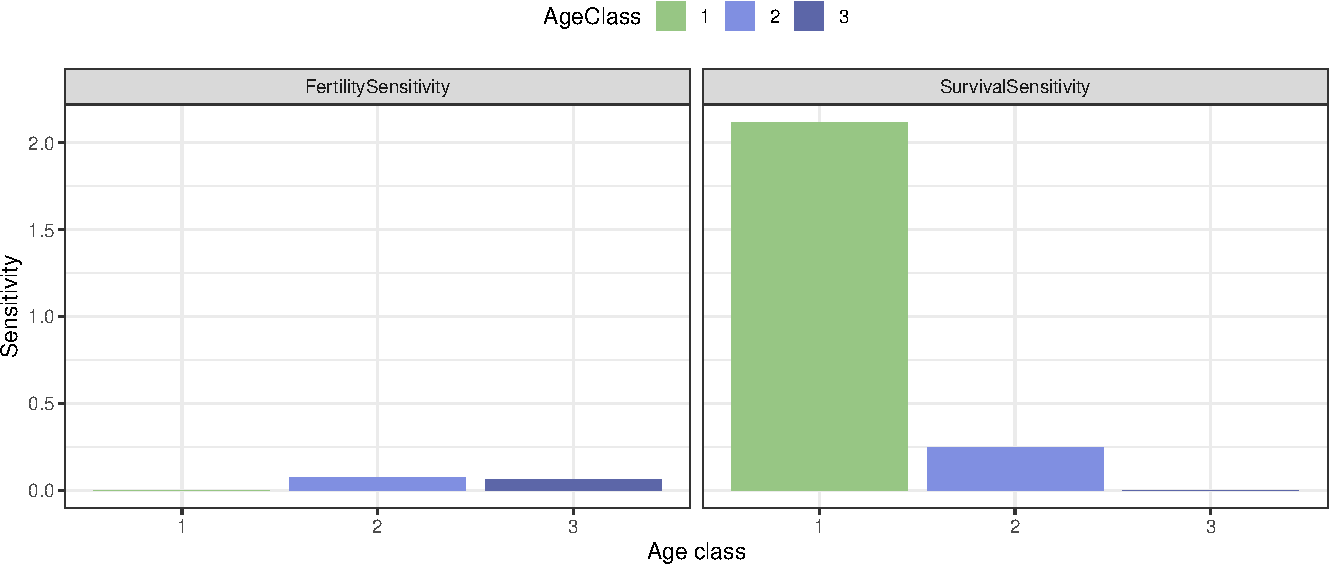
\includegraphics{DemographyCompendium_files/figure-latex/sensitivitybird1-1.pdf}
\caption{\label{fig:sensitivitybird1}Sensitivities of lambda to fertility and survival coefficients, for the bird example with post-reproductive census.}
\end{figure}

For this example, we see that the highest sensitivities are found for the survival probabilities, and in particular the first one corresponding to survival from age 0 to 1 (since we used a post-reproductive census in this example).

\hypertarget{sensitivity-to-underlying-parameters}{%
\subsection{Sensitivity to underlying parameters}\label{sensitivity-to-underlying-parameters}}

We can also calculate the sensitivity of \(\lambda\) to underlying (lower-level) parameters in the projection matrix, by applying the chain rule of derivation. If a parameter occurs in multiple entries of the matrix, we need to sum up all the corresponding sensitivities. In general, the sensitivity of \(\lambda\) to a lower level parameter \(\beta\) can be defined as

\begin{align}
\frac{\partial \lambda}{\partial \beta}=\sum_{i,j} \frac{\partial \lambda}{\partial A_{ij}} \frac{\partial A_{ij}}{\partial \beta}.
\end{align}

This kind of analysis is useful in models where the matrix elements are functions of some environmental variable, like temperature. Then we can calculate the sensitivity of \(\lambda\) to temperature through each matrix element (or sum up to age class), to understand more about how temperature affects fitness.

\hypertarget{bird-example-12}{%
\subsubsection*{Bird example}\label{bird-example-12}}
\addcontentsline{toc}{subsubsection}{Bird example}

For instance, consider the projection matrix of the bird example with a post-reproductive census (equation \eqref{eq:Postrep}):

\begin{align}
\begin{split}
\mathbf{A}=\left[\begin{matrix} f_1 & f_2 &f_3  \\ s_1 &0&0\\ 0 & s_2 &0  \\  \end{matrix}\right]=\left[\begin{matrix} 0 & p_1m_2 &p_2m_3  \\ p_0 &0&0\\ 0 & p_1 &0  \\  \end{matrix}\right].
\end{split}
\end{align}

If we want to calculate the sensitivity of \(\lambda\) to the parameter \(p_1\) (which enters element \(A_{12}\) and \(A_{32}\) in the projection matrix), we get the following expression:

\begin{align}
\frac{\partial \lambda}{\partial p_1}&=\sum_{i,j} \frac{\partial \lambda}{\partial A_{ij}} \frac{\partial A_{ij}}{\partial p_1}\\
&= v_1u_2 \frac{\partial A_{12}}{\partial p_1}+ v_3u_2 \frac{\partial A_{32}}{\partial p_1}\\
&= v_1u_2 m_2+ v_3u_2. 
\end{align}

We can use the following code to calculate and plot the sensitivites of \(\lambda\) to the survival probabilities and fecundities against actual age, assuming the post-reproductive census:

\begin{Shaded}
\begin{Highlighting}[]
\NormalTok{res }\OtherTok{\textless{}{-}} \FunctionTok{uvlambda}\NormalTok{(Abird.post)}
\NormalTok{v }\OtherTok{\textless{}{-}}\NormalTok{ res}\SpecialCharTok{$}\NormalTok{v}
\NormalTok{u }\OtherTok{\textless{}{-}}\NormalTok{ res}\SpecialCharTok{$}\NormalTok{u}

\NormalTok{m.sens }\OtherTok{\textless{}{-}} \FunctionTok{c}\NormalTok{(}\DecValTok{0}\NormalTok{, }\DecValTok{0}\NormalTok{, v[}\DecValTok{1}\NormalTok{]}\SpecialCharTok{*}\NormalTok{u[}\DecValTok{2}\NormalTok{]}\SpecialCharTok{*}\NormalTok{px[}\DecValTok{2}\NormalTok{], v[}\DecValTok{1}\NormalTok{]}\SpecialCharTok{*}\NormalTok{u[}\DecValTok{3}\NormalTok{]}\SpecialCharTok{*}\NormalTok{px[}\DecValTok{3}\NormalTok{])}\CommentTok{\#Fecundity sensitivities m0{-}m1{-}m2{-}m3}
\NormalTok{p.sens }\OtherTok{\textless{}{-}} \FunctionTok{c}\NormalTok{(v[}\DecValTok{2}\NormalTok{]}\SpecialCharTok{*}\NormalTok{u[}\DecValTok{1}\NormalTok{], v[}\DecValTok{1}\NormalTok{]}\SpecialCharTok{*}\NormalTok{u[}\DecValTok{2}\NormalTok{]}\SpecialCharTok{*}\NormalTok{mx[}\DecValTok{3}\NormalTok{]}\SpecialCharTok{+}\NormalTok{v[}\DecValTok{3}\NormalTok{]}\SpecialCharTok{*}\NormalTok{u[}\DecValTok{2}\NormalTok{], v[}\DecValTok{1}\NormalTok{]}\SpecialCharTok{*}\NormalTok{u[}\DecValTok{3}\NormalTok{]}\SpecialCharTok{*}\NormalTok{mx[}\DecValTok{4}\NormalTok{], }\DecValTok{0}\NormalTok{)}\CommentTok{\#Survival sensitivities p0{-}p1{-}p2{-}p3}

\NormalTok{sens.table.bird }\OtherTok{\textless{}{-}} \FunctionTok{data.frame}\NormalTok{(}\StringTok{"Age"}\OtherTok{=}\DecValTok{0}\SpecialCharTok{:}\DecValTok{3}\NormalTok{, }\StringTok{"mSensitivity"}\OtherTok{=}\NormalTok{m.sens, }\StringTok{"pSensitivity"}\OtherTok{=}\NormalTok{p.sens)}
\CommentTok{\#Create data frame for plotting}

\CommentTok{\#Long format for plotting:}
\NormalTok{sens.table.bird.long }\OtherTok{\textless{}{-}}\NormalTok{ sens.table.bird }\SpecialCharTok{\%\textgreater{}\%} \FunctionTok{pivot\_longer}\NormalTok{(}\FunctionTok{c}\NormalTok{(}\SpecialCharTok{{-}}\StringTok{"Age"}\NormalTok{),}
               \AttributeTok{names\_to =} \StringTok{"SensitivityTo"}\NormalTok{, }\AttributeTok{values\_to =} \StringTok{"Value"}\NormalTok{)}

\NormalTok{sens.table.bird.long}\SpecialCharTok{$}\NormalTok{Age}\OtherTok{\textless{}{-}} \FunctionTok{factor}\NormalTok{(sens.table.bird.long}\SpecialCharTok{$}\NormalTok{Age, }\AttributeTok{levels=}\FunctionTok{c}\NormalTok{(}\DecValTok{0}\NormalTok{,}\DecValTok{1}\NormalTok{,}\DecValTok{2}\NormalTok{,}\DecValTok{3}\NormalTok{))}

\CommentTok{\#Plot}

\FunctionTok{ggplot}\NormalTok{(sens.table.bird.long) }\SpecialCharTok{+} 
  \FunctionTok{geom\_col}\NormalTok{(}\FunctionTok{aes}\NormalTok{(}\AttributeTok{x=}\NormalTok{Age, }\AttributeTok{y=}\NormalTok{Value, }\AttributeTok{fill=}\NormalTok{Age ), }\AttributeTok{lwd=}\FloatTok{1.2}\NormalTok{)}\SpecialCharTok{+}
  \FunctionTok{theme\_bw}\NormalTok{() }\SpecialCharTok{+}
  \FunctionTok{facet\_wrap}\NormalTok{(}\FunctionTok{vars}\NormalTok{(SensitivityTo),}\AttributeTok{ncol=}\DecValTok{2}\NormalTok{ )}\SpecialCharTok{+}
  \FunctionTok{scale\_fill\_manual}\NormalTok{(}\AttributeTok{values=}\NormalTok{colors4)}\SpecialCharTok{+} \CommentTok{\#Add colors manually}
  \FunctionTok{labs}\NormalTok{( }\AttributeTok{x=}\StringTok{"Age (years)"}\NormalTok{, }\AttributeTok{y=}\StringTok{"Sensitivity"}\NormalTok{)}\SpecialCharTok{+} \CommentTok{\#Axis labels}
  \FunctionTok{theme}\NormalTok{(}\AttributeTok{legend.position =} \StringTok{"top"}\NormalTok{ ) }\CommentTok{\#Place legend on top}
\end{Highlighting}
\end{Shaded}

\begin{figure}
\centering
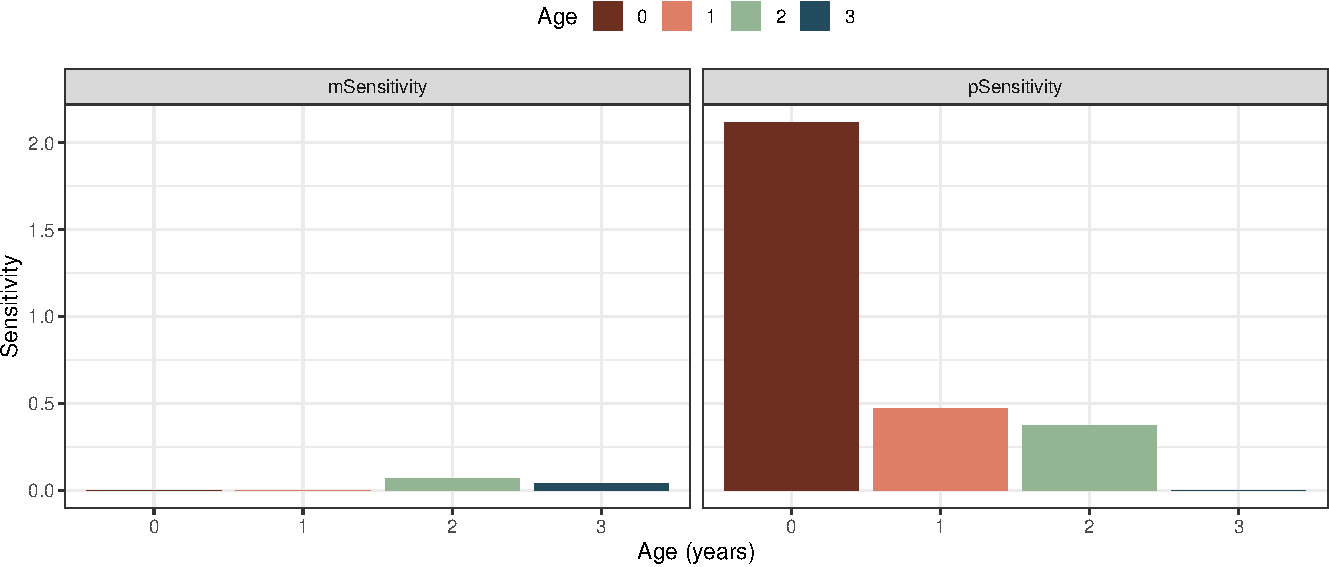
\includegraphics{DemographyCompendium_files/figure-latex/sensitivitybird2-1.pdf}
\caption{\label{fig:sensitivitybird2}Sensitivities of lambda to underlying parameters of age-specific fecundity and survival probability, for the bird example with post-reproductive census.}
\end{figure}

\hypertarget{elasticities}{%
\subsection{Elasticities}\label{elasticities}}

A closely related concept to sensitivity is the \textbf{elasticity}. The elasticity of \(\lambda\) to a projection matrix element \(A_{ij}\) is defined as the proportional change in \(\lambda\) to a proportional change in the matrix element, and is given by

\begin{align} 
\frac{\partial  \ln \lambda}{\partial \ln A_{ij}} =\frac{A_{ij}}{\lambda}\frac{\partial  \lambda}{\partial A_{ij}}=\frac{A_{ij}}{\lambda} v_{i}u_{j}=\frac{A_{ij}}{\lambda} S_{ij}=.
\end{align}

The function below returns the elasticity matrix for a given projection matrix \(\mathbf{A}\).

\begin{Shaded}
\begin{Highlighting}[]
\NormalTok{elasticity.matrix }\OtherTok{\textless{}{-}} \ControlFlowTok{function}\NormalTok{(MatA, }\AttributeTok{zeroes=}\NormalTok{T)\{}
\NormalTok{  res }\OtherTok{\textless{}{-}} \FunctionTok{uvlambda}\NormalTok{(}\AttributeTok{MatA=}\NormalTok{MatA)}
\NormalTok{  sensmat }\OtherTok{\textless{}{-}} \FunctionTok{t}\NormalTok{(res}\SpecialCharTok{$}\NormalTok{u}\SpecialCharTok{\%*\%}\NormalTok{res}\SpecialCharTok{$}\NormalTok{v)}
  \ControlFlowTok{if}\NormalTok{ (zeroes}\SpecialCharTok{==}\NormalTok{T)\{}
\NormalTok{    sensmat }\OtherTok{\textless{}{-}} \FunctionTok{ifelse}\NormalTok{ (MatA}\SpecialCharTok{==}\DecValTok{0}\NormalTok{, }\DecValTok{0}\NormalTok{, sensmat)}
\NormalTok{  \}}
\NormalTok{ sensmat}\SpecialCharTok{*}\NormalTok{MatA}\SpecialCharTok{/}\NormalTok{res}\SpecialCharTok{$}\NormalTok{lam }
\NormalTok{\}}
\end{Highlighting}
\end{Shaded}

The elasticity to a lower-level parameter \(\beta\) can be found in a similar way, as

\begin{align} 
\frac{\partial  \ln \lambda}{\partial \ln \beta} =\frac{\beta}{\lambda}\frac{\partial  \lambda}{\partial \beta}.
\end{align}

\hypertarget{bird-example-13}{%
\subsubsection*{Bird example}\label{bird-example-13}}
\addcontentsline{toc}{subsubsection}{Bird example}

Continuing with the bird example with a post-reproductive census, the elasticities to age-specific fecundity and survival probability can be found as follows, using the sensitivities found in the previous section:

\begin{Shaded}
\begin{Highlighting}[]
\NormalTok{m.elas }\OtherTok{\textless{}{-}}\NormalTok{ mx}\SpecialCharTok{/}\NormalTok{lambda.bird.post}\SpecialCharTok{*}\NormalTok{m.sens }\CommentTok{\#Fecundity elasticities m0{-}m1{-}m2{-}m3}
\NormalTok{p.elas }\OtherTok{\textless{}{-}}\NormalTok{ px}\SpecialCharTok{/}\NormalTok{lambda.bird.post}\SpecialCharTok{*}\NormalTok{p.sens }\CommentTok{\#Survival elasticities p0{-}p1{-}p2{-}p3}
 
\NormalTok{elas.table.bird }\OtherTok{\textless{}{-}} \FunctionTok{data.frame}\NormalTok{(}\StringTok{"Age"}\OtherTok{=}\DecValTok{0}\SpecialCharTok{:}\DecValTok{3}\NormalTok{, }\StringTok{"mElasticity"}\OtherTok{=}\NormalTok{m.elas, }\StringTok{"pElasticity"}\OtherTok{=}\NormalTok{p.elas)}
\CommentTok{\#Create data frame for plotting}

\CommentTok{\#Long format for plotting:}
\NormalTok{elas.table.bird.long }\OtherTok{\textless{}{-}}\NormalTok{ elas.table.bird }\SpecialCharTok{\%\textgreater{}\%} \FunctionTok{pivot\_longer}\NormalTok{(}\FunctionTok{c}\NormalTok{(}\SpecialCharTok{{-}}\StringTok{"Age"}\NormalTok{),}
               \AttributeTok{names\_to =} \StringTok{"ElasticityTo"}\NormalTok{, }\AttributeTok{values\_to =} \StringTok{"Value"}\NormalTok{)}

\NormalTok{elas.table.bird.long}\SpecialCharTok{$}\NormalTok{Age}\OtherTok{\textless{}{-}} \FunctionTok{factor}\NormalTok{(elas.table.bird.long}\SpecialCharTok{$}\NormalTok{Age, }\AttributeTok{levels=}\DecValTok{0}\SpecialCharTok{:}\DecValTok{3}\NormalTok{)}
\CommentTok{\#Plot}
\FunctionTok{ggplot}\NormalTok{(elas.table.bird.long) }\SpecialCharTok{+} 
  \FunctionTok{geom\_col}\NormalTok{(}\FunctionTok{aes}\NormalTok{(}\AttributeTok{x=}\NormalTok{Age, }\AttributeTok{y=}\NormalTok{Value, }\AttributeTok{fill=}\NormalTok{Age ), }\AttributeTok{lwd=}\FloatTok{1.2}\NormalTok{)}\SpecialCharTok{+}
  \FunctionTok{theme\_bw}\NormalTok{() }\SpecialCharTok{+}
  \FunctionTok{facet\_wrap}\NormalTok{(}\FunctionTok{vars}\NormalTok{(ElasticityTo),}\AttributeTok{ncol=}\DecValTok{2}\NormalTok{ )}\SpecialCharTok{+}
  \FunctionTok{scale\_fill\_manual}\NormalTok{(}\AttributeTok{values=}\NormalTok{colors4)}\SpecialCharTok{+} \CommentTok{\#Add colors manually}
  \FunctionTok{labs}\NormalTok{( }\AttributeTok{x=}\StringTok{"Age (years)"}\NormalTok{, }\AttributeTok{y=}\StringTok{"Elasticity"}\NormalTok{)}\SpecialCharTok{+} \CommentTok{\#Axis labels}
  \FunctionTok{theme}\NormalTok{(}\AttributeTok{legend.position =} \StringTok{"top"}\NormalTok{ ) }\CommentTok{\#Place legend on top}
\end{Highlighting}
\end{Shaded}

\begin{figure}
\centering
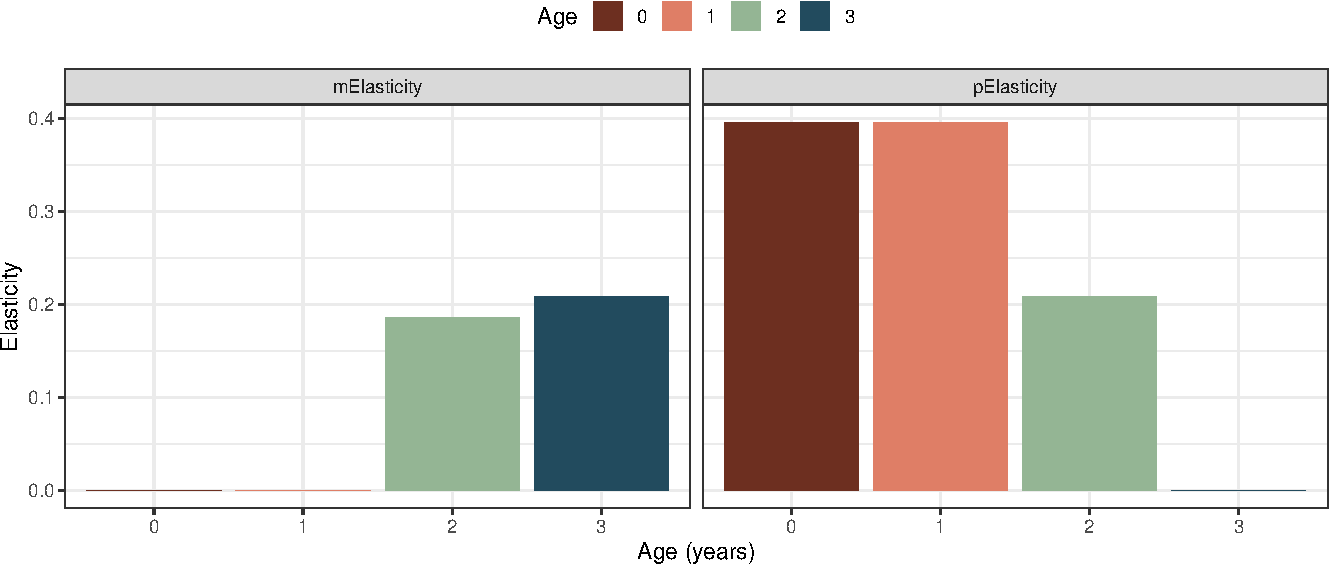
\includegraphics{DemographyCompendium_files/figure-latex/elasticitybird-1.pdf}
\caption{\label{fig:elasticitybird}Elasticities of lambda to underlying parameters of age-specific fecundity and survival probability, for the bird example with post-reproductive census.}
\end{figure}

Note that the elasticities of fecundities \(m_x\) and survival probabilities \(p_x\) are more similar than the sensitivites. This is because the elasticities represent proportional changes in \(\lambda\) while sensitivities represent absolute changes, and fecundity and survival are variables with different scales. We should always keep this in mind when interpreting sensitivities (and elasticities), as an absolute change in fecundity is not the same as the same absolute change in a survival probability. Although elasticities measure proportional effects, they are not better than sensitivities in this sense (which is sometimes claimed), and still need to be interpreted carefully.

\hypertarget{senescence}{%
\section{Senescence}\label{senescence}}

The sensitivities of \(\lambda\) with respect to age-specific survival and fecundities are important because (among other things) they measure selection pressures. More generally, a \textbf{selection gradient} of a trait (survival probability and fertility are also traits) is defined as the slope of fitness as a function of the trait. For a trait with value \(\theta\), the selection gradient is the partial derivative:

\begin{align} 
\text{Gradient}=\frac{\partial \text{Fitness}}{\partial \theta}.
\end{align}
If the trait is a vector, such as the vector of age-specific survival probabilities \(p_i\), the gradient is also a vector.

Based on the Euler-Lotka equation, \citet{Hamilton1} derived the selection gradient of \(r=\ln\lambda\) on (log) age-specific survival probability \(p_x\):

\begin{align} 
\frac{\partial r}{\partial \ln p_x}&=\frac{\sum_{y=x}^ke^{-ry}l_ym_y}{T_C},
\end{align}
where \(T_C\) is the cohort generation time as defined in chapter \ref{s02-life-tables}. The selection gradient on age-specific fecundity \(m_x\) is given by

\begin{align} 
\frac{\partial r}{\partial m_x}&=\frac{e^{-rx}l_x}{T_C}.
\end{align}
The selection gradient on survival will decline with age \(x\), after the age at first reproduction. For fecundity, the selection gradient will usually decrease with age, except in strongly declining populations: If \(r\) is sufficiently negative relative to survival probability so that the stable age distribution increases with age, then the selection gradient can increase. This situation is unlikely to be common or persist for long time periods.

Because the selection gradients (nearly) always decline with age, \citet{Hamilton1} concluded that senescence is inevitable for any conceivable organism. With his selection gradients, Hamilton formalized the arguments previously given regarding mutation accumulation hypothesis \citep{Medawar1}, and the antagonistic pleiotropy hypothesis \citep{Williams1}. Any change in the environment that causes the selection gradients to fall off more rapidly with age should select for increased senescence, while changes that make the slope less steep should select for reduced senescence.

\hypertarget{bird-example-14}{%
\subsubsection*{Bird example}\label{bird-example-14}}
\addcontentsline{toc}{subsubsection}{Bird example}

We can plot these selection gradients for the bird example (note that we now use the life table from chapter \ref{s02-life-tables}):

\begin{Shaded}
\begin{Highlighting}[]
\NormalTok{res }\OtherTok{\textless{}{-}} \FunctionTok{uvlambda}\NormalTok{(Abird.post)}
\NormalTok{r }\OtherTok{\textless{}{-}} \FunctionTok{log}\NormalTok{(res}\SpecialCharTok{$}\NormalTok{lam)}
 
\NormalTok{dr.dp }\OtherTok{\textless{}{-}} \FunctionTok{rev}\NormalTok{(}\FunctionTok{cumsum}\NormalTok{(}\FunctionTok{rev}\NormalTok{(}\FunctionTok{exp}\NormalTok{(}\SpecialCharTok{{-}}\NormalTok{r}\SpecialCharTok{*}\NormalTok{x)}\SpecialCharTok{*}\NormalTok{lx}\SpecialCharTok{*}\NormalTok{mx)))}\SpecialCharTok{/}\NormalTok{TC\_Bird }\CommentTok{\#Calculating the reverse cumulative sum for dr.dp can also be done with a for loop}
\NormalTok{dr.dm }\OtherTok{\textless{}{-}}  \FunctionTok{exp}\NormalTok{(}\SpecialCharTok{{-}}\NormalTok{r}\SpecialCharTok{*}\NormalTok{x)}\SpecialCharTok{*}\NormalTok{lx}\SpecialCharTok{/}\NormalTok{TC\_Bird}

\NormalTok{bird.table }\OtherTok{\textless{}{-}} \FunctionTok{data.frame}\NormalTok{(x, dr.dp, dr.dm)}

\CommentTok{\#long format for plotting:}
\NormalTok{bird.table.long }\OtherTok{\textless{}{-}}\NormalTok{ bird.table }\SpecialCharTok{\%\textgreater{}\%} \FunctionTok{pivot\_longer}\NormalTok{(}\FunctionTok{c}\NormalTok{( dr.dp, dr.dm),}
               \AttributeTok{names\_to =} \StringTok{"Sensitivity"}\NormalTok{, }\AttributeTok{values\_to =} \StringTok{"Value"}\NormalTok{)}
 
\NormalTok{bird.table.long}\SpecialCharTok{$}\NormalTok{Age }\OtherTok{\textless{}{-}} \FunctionTok{factor}\NormalTok{(bird.table.long}\SpecialCharTok{$}\NormalTok{x, }\AttributeTok{levels=}\DecValTok{0}\SpecialCharTok{:}\DecValTok{3}\NormalTok{)}

\FunctionTok{ggplot}\NormalTok{(bird.table.long) }\SpecialCharTok{+} 
  \FunctionTok{geom\_col}\NormalTok{(}\FunctionTok{aes}\NormalTok{(}\AttributeTok{x=}\NormalTok{Age, }\AttributeTok{y=}\NormalTok{Value , }\AttributeTok{fill=}\NormalTok{Age) , }\AttributeTok{lwd=}\FloatTok{1.2}\NormalTok{)}\SpecialCharTok{+}
  \FunctionTok{facet\_wrap}\NormalTok{(}\FunctionTok{vars}\NormalTok{(Sensitivity))}\SpecialCharTok{+}
  \FunctionTok{scale\_fill\_manual}\NormalTok{(}\AttributeTok{values=}\NormalTok{colors4)}\SpecialCharTok{+}
  \FunctionTok{theme\_bw}\NormalTok{() }\SpecialCharTok{+}
  \FunctionTok{labs}\NormalTok{( }\AttributeTok{x=}\StringTok{"Age (year)"}\NormalTok{, }\AttributeTok{y=}\StringTok{"Sensitivity of r"}\NormalTok{)}\SpecialCharTok{+}
   \FunctionTok{theme}\NormalTok{(}\AttributeTok{legend.position =} \StringTok{"none"}\NormalTok{ )}\CommentTok{\#Drop legend}
\end{Highlighting}
\end{Shaded}

\begin{figure}
\centering
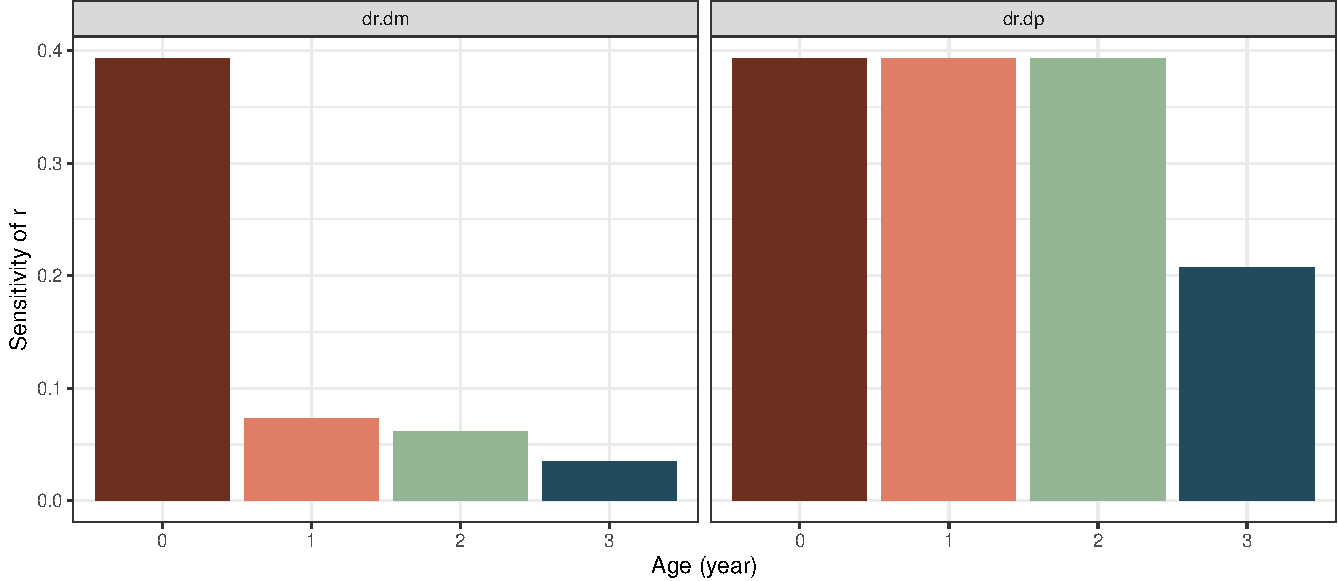
\includegraphics{DemographyCompendium_files/figure-latex/birdgradients-1.pdf}
\caption{\label{fig:birdgradients}Selection gradients on fecundity and survival probability in the bird example, based on the life table from chapter 2.}
\end{figure}

We see that also for the bird example the selection gradients decline with age, \(\frac{\partial r}{\partial p_x}\) after the age of first reproduction (here 2 years) and \(\frac{\partial r}{\partial m_x}\) for all ages.

\hypertarget{the-effect-of-extrinsic-mortality-on-senescence}{%
\subsection*{The effect of extrinsic mortality on senescence}\label{the-effect-of-extrinsic-mortality-on-senescence}}
\addcontentsline{toc}{subsection}{The effect of extrinsic mortality on senescence}

\citet{Williams1} suggested that increased extrinsic mortality could be such a factor leading to steeper gradients, and that simply living in a more risky environment (e.g.~with many predators) should select for more rapid senescence. This may seem intuitive, however other researchers have shown that if the extrinsic mortality is age-independent, it has no effect on the slope of the selection gradient and thus no effect on senescence \citep{Hamilton1, Caswell7, Wensink1}. The reason is that extra mortality will affect not only the the survivorship \(l_x\), but also parameters that depend on it such as \(r\) and the stable age structure. It turns out that when the added mortality is age-independent, effects cancel each other out in the numerator and denominator of Hamilton's selection gradient, so that there is no effect on senescence. If the extrinsic mortality is age-dependent, however (for instance if only younger individuals are exposed to increased predation), the selection gradients and senescence will also be affected. In general (and all else being equal), increased mortality in early life will then select for reduced senescence, while increased mortality in late life selects for increased senescence.

An associated common misconception is that senescence occurs `because few individuals survive to old age', and that old-age individuals are therefore evolutionarily unimportant. This argument ignores the role of reproduction: Patterns of senescence cannot be described by declines in survivorship with age alone (the \(l_x\) curve; see chapter \ref{s02-life-tables}), because life histories are shaped by both survival and reproduction. Think of the life history of a large tree species: Only few individuals survive from seedling to old age, yet senescence is hardly present in many of these species. Even in the hypothetical situation of a species with no mortality at all (a flat \(l_x\)-curve), the selection gradients would still decline with age, because of reproduction leading to ever-increasing numbers of newborn individuals compared to older ages.

\hypertarget{LTRE}{%
\section{Life table response experiments (LTRE)}\label{LTRE}}

Sometimes we want to compare larger differences in \(\lambda\) between two or more different conditions - for instance for populations living in different environments, or populations that have experienced different management treatments. The purpose of a life table response experiment (LTRE) is to understand how different projection matrix elements (or underlying parameters) have contributed to the difference in \(\lambda\). \citet{Caswell1}, who introduced this method, describes it in more detail. LTRE analysis is inspired by experimental approaches and analysis of variance (ANOVA), but does not require any actual experiments to take place. The `experiment' can also be for instance an observed change in the projection matrix after a sudden environmental change, or a management decision.

\hypertarget{general-description-of-ltre-approach}{%
\subsection{General description of LTRE approach}\label{general-description-of-ltre-approach}}

To do an LTRE analysis to compare \(\lambda\) in two environments, we first define a \textbf{reference matrix} \(\mathbf{A}^{(r)}\), defining the reference life history with growth rate \(\lambda^{(r)}\). Now assume that we want to compare this to another matrix \(\mathbf{A}^{(m)}\) for the same species, where the vital rates are different e.g.~because of some environmental impact. This matrix is called a \textbf{treatment matrix} and has a corresponding \(\lambda^{(m)}\). We want to understand how much of the difference between \(\lambda^{(m)}-\lambda^{(r)}\) is coming from each vital rate. To do this, we first define two useful matrices \citep{Caswell1}:

\begin{itemize}
\item
  \(\mathbf{A}^*=\frac{1}{2}\left(\mathbf{A}^{(m)}+\mathbf{A}^{(r)}\right)\) defines the `halfway matrix', i.e.~a matrix where each element is the average of the corresponding elements in \(\mathbf{A}^{(m)}\) and \(\mathbf{A}^{(r)}\).
\item
  \(\mathbf{D}=\mathbf{A}^{(m)}-\mathbf{A}^{(r)}\) is the `difference matrix', where each element corresponds to the
  difference between the corresponding elements in \(\mathbf{A}^{(m)}\) and \(\mathbf{A}^{(r)}\).
\end{itemize}

Now we can write \(\lambda^{(m)}\) as a function of \(\lambda^{(r)}\) (the reference value), plus a sum of difference contributions from each matrix element, weighted by the senstivity of \(\lambda\) to that element \citep{Caswell1}:

\begin{align}
\lambda^{(m)}\approx \lambda^{(r)}+\sum_{i,j}d_{ij}\left.\frac{\partial\lambda}{\partial a_{ij}}\right|_{\mathbf{A}^*},
\label{eq:LTREeq}
\end{align}

where the sensitivities are calculated for the matrix \(\mathbf{A}^*\). A common output of such an analysis is to plot these contributions side by side. Doing a life table response analysis for \(\lambda\) involves the following steps:

\begin{enumerate}
\def\labelenumi{\arabic{enumi})}
\item
  Define all the relevant projection matrices for each treatment / environment and define a reference matrix, and calculate \(\lambda\) for each.
\item
  Calculate \(\mathbf{A}^*\) and \(\mathbf{D}\),
\item
  Calculate the sensitivity matrix corresponding to the matrix \(\mathbf{A}^*\),
\item
  Calculate the contributions from each vital rate to the difference in \(\lambda\) according to the sum defined above.
\end{enumerate}

Note that LTRE analyses can also be done for more than one comparison environment, using the same approach as described here.

\hypertarget{ltre-and-sensitivity-analyses}{%
\subsection{LTRE and sensitivity analyses}\label{ltre-and-sensitivity-analyses}}

An LTRE analysis is \emph{retrospective}, aiming to explain observed differences in \(\lambda\), while the sensitivity analysis is \emph{prospective}, aiming to explain potential future responses of \(\lambda\) to perturbations of the matrix elements \citep{Caswell1}. The two can give very different answers in terms of which matrix element is the `most important' (largest sensitivity or largest LTRE contribution).

\hypertarget{bird-example-15}{%
\subsubsection*{Bird example}\label{bird-example-15}}
\addcontentsline{toc}{subsubsection}{Bird example}

We can demonstrate the LTRE analysis using the bird example. Here we will again assume a pre-reproductive census (you can do the same analysis for the post-reproductive model). The matrix defined in equation \eqref{eq:Prerep} is now the reference matrix:

\begin{align*}
\mathbf{A}^{(r)}=\left[\begin{matrix} 0 &0.6 &1.2  \\ 0.9 &0&0\\ 0 & 0.6 &0  \\  \end{matrix}\right].
\end{align*}

Remember that with this projection matrix we get a value of \(\lambda^{(r)}\approx\) 1.07.

Now assume that the bird was affected by increased predation, leading to a different projection matrix

\begin{align*}
\mathbf{A}^{(m)}=\left[\begin{matrix} 0 &0.4 &1   \\ 0.8 &0&0\\ 0 & 0.4 &0  \\  \end{matrix}\right].
\end{align*}

For this treatment matrix we can calculate the following value of \(\lambda^{(m)}\) and its difference to the reference:

\begin{Shaded}
\begin{Highlighting}[]
\NormalTok{AmatBirdR }\OtherTok{\textless{}{-}}\NormalTok{  Abird.pre  }\CommentTok{\#Reference matrix }
\NormalTok{AmatBirdM }\OtherTok{\textless{}{-}} \FunctionTok{Create.Amat}\NormalTok{(}\AttributeTok{Svec=}\FunctionTok{c}\NormalTok{(.}\DecValTok{8}\NormalTok{,.}\DecValTok{5}\NormalTok{,.}\DecValTok{0}\NormalTok{), }\AttributeTok{Fvec=}\FunctionTok{c}\NormalTok{(}\DecValTok{0}\NormalTok{,.}\DecValTok{5}\NormalTok{,}\DecValTok{1}\NormalTok{ ))  }\CommentTok{\#Define treatment matrix}

\NormalTok{lambdaR}\OtherTok{\textless{}{-}} \FunctionTok{uvlambda}\NormalTok{(AmatBirdR)}\SpecialCharTok{$}\NormalTok{lam }\CommentTok{\#Lambda in reference environment}
\NormalTok{lambdaM }\OtherTok{\textless{}{-}} \FunctionTok{uvlambda}\NormalTok{(AmatBirdM)}\SpecialCharTok{$}\NormalTok{lam }\CommentTok{\#Lambda in treatment environment}

\NormalTok{lamDiff }\OtherTok{\textless{}{-}}\NormalTok{ lambdaM}\SpecialCharTok{{-}}\NormalTok{lambdaR}\CommentTok{\#Difference in lambda}
\end{Highlighting}
\end{Shaded}

In the environment with increased predation, we get \(\lambda^{(m)}\approx\) 0.915. This leads to a quite large difference of \(\lambda^{(m)}-\lambda^{(r)}\approx\) -0.155. Now we are interested in which matrix element contributes the most to this difference in \(\lambda\).

First we calculate the halway matrix and difference matrix:

\begin{Shaded}
\begin{Highlighting}[]
\NormalTok{HalfwaymatBird }\OtherTok{\textless{}{-}}\NormalTok{ (AmatBirdM}\SpecialCharTok{+}\NormalTok{AmatBirdR)}\SpecialCharTok{/}\DecValTok{2}
\NormalTok{DiffmatBird }\OtherTok{\textless{}{-}}\NormalTok{ AmatBirdM}\SpecialCharTok{{-}}\NormalTok{AmatBirdR}

\NormalTok{DiffmatBird}
\end{Highlighting}
\end{Shaded}

\begin{verbatim}
##      [,1] [,2] [,3]
## [1,]  0.0 -0.1 -0.2
## [2,] -0.1  0.0  0.0
## [3,]  0.0 -0.1  0.0
\end{verbatim}

The largest difference is found for the fertility of age class 3. But this is not necessarily the element contributing the most to the difference in \(\lambda\).

To calculate the contributions to \(\lambda\) we first need the sensitivity matrix calcalated for the halfway matrix \(\mathbf{A^*}\). Then we can apply equation \eqref{eq:LTREeq} and plot the components of this sum:

\begin{Shaded}
\begin{Highlighting}[]
\NormalTok{SensHalfwaymatBird }\OtherTok{\textless{}{-}} \FunctionTok{sensitivity.matrix}\NormalTok{(HalfwaymatBird)}
 
\NormalTok{LTREMat }\OtherTok{\textless{}{-}}\NormalTok{ DiffmatBird}\SpecialCharTok{*}\NormalTok{ SensHalfwaymatBird }\CommentTok{\#Matrix corresponding to elements inside the sum of the LTRE equation}

\NormalTok{FertilityContributions }\OtherTok{\textless{}{-}}\NormalTok{ LTREMat[}\DecValTok{1}\NormalTok{,] }\CommentTok{\#Fertility components}
\NormalTok{SurvivalContributions }\OtherTok{\textless{}{-}} \FunctionTok{c}\NormalTok{(LTREMat[}\DecValTok{2}\NormalTok{,}\DecValTok{1}\NormalTok{], LTREMat[}\DecValTok{3}\NormalTok{,}\DecValTok{2}\NormalTok{], LTREMat[}\DecValTok{3}\NormalTok{,}\DecValTok{3}\NormalTok{]) }\CommentTok{\#Last element will be zero \#Survival components}

\NormalTok{LTRE.table }\OtherTok{\textless{}{-}} \FunctionTok{data.frame}\NormalTok{(}\AttributeTok{AgeClass=}\FunctionTok{factor}\NormalTok{(}\DecValTok{1}\SpecialCharTok{:}\DecValTok{3}\NormalTok{), FertilityContributions, SurvivalContributions)}

\CommentTok{\#long format for plotting:}
\NormalTok{LTRE.table.long }\OtherTok{\textless{}{-}}\NormalTok{ LTRE.table }\SpecialCharTok{\%\textgreater{}\%} \FunctionTok{pivot\_longer}\NormalTok{(}\FunctionTok{c}\NormalTok{( FertilityContributions, SurvivalContributions),}
               \AttributeTok{names\_to =} \StringTok{"Component"}\NormalTok{, }\AttributeTok{values\_to =} \StringTok{"Value"}\NormalTok{)}
 
\FunctionTok{ggplot}\NormalTok{(LTRE.table.long) }\SpecialCharTok{+} 
  \FunctionTok{geom\_col}\NormalTok{(}\FunctionTok{aes}\NormalTok{(}\AttributeTok{x=}\NormalTok{AgeClass, }\AttributeTok{y=}\NormalTok{Value , }\AttributeTok{fill=}\NormalTok{AgeClass) , }\AttributeTok{lwd=}\FloatTok{1.2}\NormalTok{)}\SpecialCharTok{+}
  \FunctionTok{facet\_wrap}\NormalTok{(}\FunctionTok{vars}\NormalTok{(Component))}\SpecialCharTok{+}
  \FunctionTok{scale\_fill\_manual}\NormalTok{(}\AttributeTok{values=}\NormalTok{colors3)}\SpecialCharTok{+}
  \FunctionTok{theme\_bw}\NormalTok{() }\SpecialCharTok{+}
  \FunctionTok{labs}\NormalTok{( }\AttributeTok{x=}\StringTok{"Age class"}\NormalTok{, }\AttributeTok{y=}\StringTok{"Contribution to lambda difference"}\NormalTok{)}\SpecialCharTok{+}
    \FunctionTok{theme}\NormalTok{(}\AttributeTok{legend.position =} \StringTok{"none"}\NormalTok{ )}\CommentTok{\#Drop legend}
\end{Highlighting}
\end{Shaded}

\begin{figure}
\centering
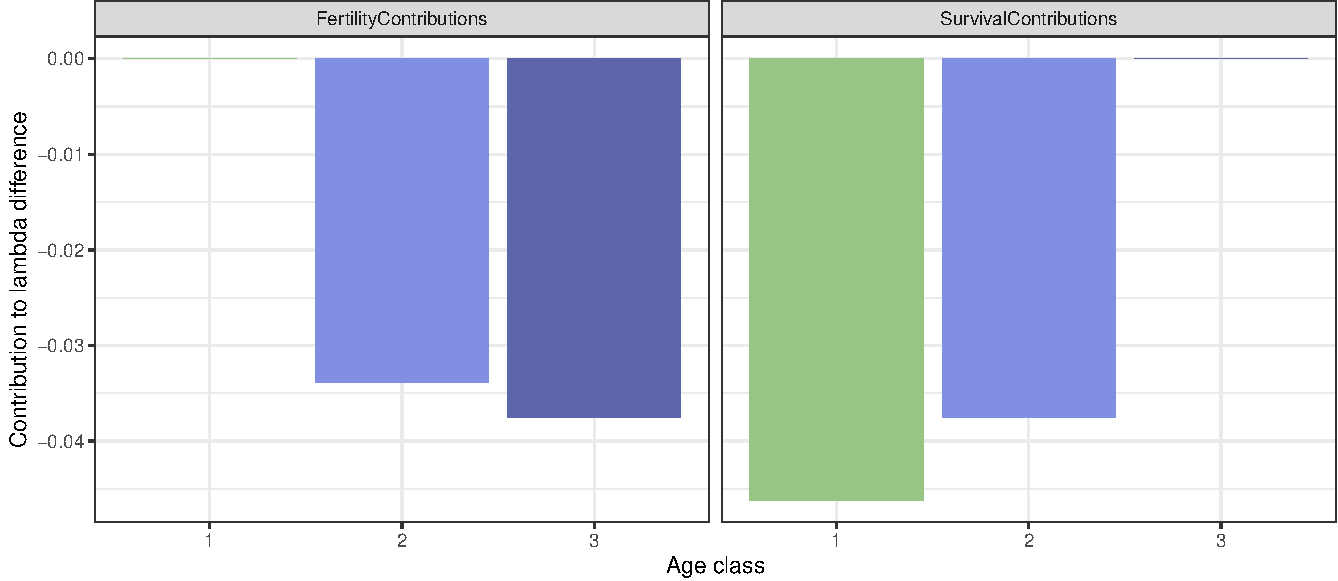
\includegraphics{DemographyCompendium_files/figure-latex/birdLTRE-1.pdf}
\caption{\label{fig:birdLTRE}LTRE components for the bird example, corresponding to fertility and survival coefficients in the prereproductive census model, compared to an alternative model with increased predation.}
\end{figure}

Here we see that the element contribution most to the difference \(\lambda^{(m)}-\lambda^{(r)}\) is the survival probability of age class 1, followed by fertility of age class 3, survival of age class 2, and fertility of age class 2.

We can check the approximation by summing up the LTRE contributions:

\begin{Shaded}
\begin{Highlighting}[]
\NormalTok{sumDiff }\OtherTok{\textless{}{-}} \FunctionTok{sum}\NormalTok{(LTREMat)}
\NormalTok{Vek }\OtherTok{\textless{}{-}} \FunctionTok{c}\NormalTok{(lamDiff, sumDiff)}
\FunctionTok{names}\NormalTok{(Vek) }\OtherTok{\textless{}{-}} \FunctionTok{c}\NormalTok{(}\StringTok{"Exact"}\NormalTok{, }\StringTok{"LTREsum"}\NormalTok{)}
\NormalTok{Vek}
\end{Highlighting}
\end{Shaded}

\begin{verbatim}
##      Exact    LTREsum 
## -0.1552903 -0.1552733
\end{verbatim}

These values are quite similar, indicating that the LTRE approximation is ok.

In this example predation had a negative effect on projection matrix elements, but it is often the case that the effect of a perturbation is negative on some elements, and positive on others. The total difference in \(\lambda\) can then be quite small despite large effects on each matrix element, and an LTRE analysis is important to reveal the opposing effects.

\hypertarget{exercises-2}{%
\section{Exercises}\label{exercises-2}}

For suggested solutions, see appendix \ref{s09-Solutions}.

\hypertarget{exercise-3.1}{%
\subsection*{Exercise 3.1}\label{exercise-3.1}}
\addcontentsline{toc}{subsection}{Exercise 3.1}

Draw the post-reproductive life cycle graph for the bird example (projection matrix shown in equation \eqref{eq:Postrep}).

\hypertarget{exercise-3.2}{%
\subsection*{Exercise 3.2}\label{exercise-3.2}}
\addcontentsline{toc}{subsection}{Exercise 3.2}

Start with the complete life table you calculated in Exercise 2.2.

\begin{enumerate}
\def\labelenumi{\arabic{enumi}.}
\item
  Draw a life cycle graph for this population (on paper or using a drawing program), assuming a \textbf{pre-reproductive census}.
\item
  Calculate the vector of fertility coefficients \(f_i\) and survival probabilities \(s_i\), assuming a pre-reproductive census.
\item
  Define the Leslie matrix \(\mathbf{A}\) in R for this population (still assuming pre-reproductive census), as well as its two components \(\mathbf{U}\) and \(\mathbf{F}\).
\item
  Use the Leslie matrix to project the growth of each age class over 30 time steps, and plot the result.
\item
  Calculate the long-term growth rate \(\lambda\), the net reproductive rate \(R_0\) and the generation time \(\mathbf{G}\) using the three matrices you defined in task 3. Do you get the same values as in exercise 2.2? If not, can you explain the difference?
\item
  Calculate and plot the stable age structure \(\mathbf{u}\) and reproductive values \(\mathbf{v}\) for the population. Explain the biological meaning of the results.
\item
  Assume that you could increase reproduction by multiplying the entire vector of fecundities \(m_x\) by some constant factor \(c\). How large should this factor be to achieve a long-term growth rate \(\lambda\) above 1? Update the three matrices \(\mathbf{A}\), \(\mathbf{U}\) and \(\mathbf{F}\) using the new fecundity values (give them new names in R) and do the same analysis as above for the new model. What happened to \(R_0\) and \(G\)? How did the resulting stable structure and reproductive values change?
\item
  This time increase the annual survival probability vector \(p_x\) by some factor, instead of \(m_x\), to get a \(\lambda>1\). Is the resulting survival probability vector biologically realistic? Why/why not?
\item
  Do the exercise of point 1-8 again, but this time change from a pre-reproductive to post-reproductive census model. Which results have now changed, and which have not?
\end{enumerate}

\hypertarget{s04-Stage}{%
\chapter{Stage structured models}\label{s04-Stage}}

The life table and associated parameters defined in the previous chapters apply only to age structured populations. However, the methods you learned for matrix models can be used with any projection matrix \(\mathbf{A}\) (provided it fulfills certain mathematical assumptions). The only difference is that the results refer to stages instead of age class. This chapter will present a general stage structured matrix model and show how to build the projection matrix from four main components describing transitions, survival probability and fertility. We will then go through some main sources of stage structure and consider examples.

\hypertarget{learning-goals-3}{%
\section{Learning goals}\label{learning-goals-3}}

\begin{itemize}
\item
  Understand the key components of a stage structured matrix model.
\item
  Get the vectors of survival probability and fertility coefficients from the matrices \(\mathbf{U}\) and \(\mathbf{F}\) .
\item
  Discuss some main sources of stage structure.
\item
  Draw a life cycle graph for any stage structured model.
\item
  Apply methods from chapter \ref{s03-MatrixModels} to stage structured matrix models
\item
  Define a simple integral projection model for size structured populations.
\end{itemize}

\hypertarget{general-stage-structured-matrix-model}{%
\section{General stage structured matrix model}\label{general-stage-structured-matrix-model}}

We will now extend the age structured model to the general case of stage structured models, which can be adapted to describe many different kinds of stage structure. As shown by \citet{Vindenes2020}, the general projection matrix \(\mathbf{A}\) can be decomposed into four main components:

\begin{align}
\mathbf{A}&=\mathbf{U}+\mathbf{F}=\mathbf{G}\text{Diag}(\mathbf{s})+\mathbf{Q}\text{Diag}(\mathbf{f}),
\label{eq:General}
\end{align}

where \(\mathbf{G}\) is a transition matrix containing the transition probabilities \(g_{ij}\) from stage \(j\) to stage \(i\) per time step (column sums of this matrix should all be 1), \(\mathbf{s}\) is the vector of survival probabilities (survival from current to next time step) in each stage, \(\mathbf{Q}\) is a matrix containing the probabilities \(q_{ij}\) that an offspring produced in stage \(j\) is assigned to stage \(i\) at birth (columns should sum to 1), and \(\mathbf{f}\) is the vector of fertilities per stage, i.e.~the mean number of offspring contributed by an individual to next time step's population.

For a population with 3 stages, the elements of each matrix in equation \eqref{eq:General} are given by

\begin{align*}
&\left[\begin{matrix} 
g_{11}s_1+q_{11}f_1  & g_{12}s_2+q_{12}f_2 & g_{13}s_3+q_{13}f_3\\ 
g_{21}s_1+q_{21}f_1  & g_{22}s_2+q_{22}f_2 & g_{23}s_3+q_{23}f_3\\ 
g_{31}s_1+q_{31}f_1  & g_{32}s_2+q_{32}f_2 & g_{33}s_3+q_{33}f_3 
\end{matrix}\right]\\
=
&\left[\begin{matrix} 
g_{11} & g_{12}& g_{13} \\ 
g_{21} & g_{22}& g_{33} \\ 
g_{31} & g_{32}& g_{33}  
\end{matrix}\right]
\left[\begin{matrix} 
s_1 & 0& 0 \\ 
0 & s_2&0 \\ 
0 & 0& s_3 
\end{matrix}\right]+
\left[\begin{matrix} 
q_{11} & q_{12}& q_{13} \\ 
q_{21} & q_{22}& q_{33} \\ 
q_{31} & q_{32}& q_{33}  
\end{matrix}\right]
\left[\begin{matrix} 
f_1 & 0& 0 \\ 
0 & f_2&0 \\ 
0 & 0& f_3 
\end{matrix}\right].
\end{align*}

The stage-specific survival and fertility coefficients are the same as before: The survival coefficient \(s_j\) represent the probability that an individual in stage \(j\) will survive until the next time step. The fertility coefficient \(f_j\) represent the average number of offspring contributed by an individual in stage \(j\) to the population in the next time step. Census time still plays a role in the definition of the fertility coefficient from underlying parameters.

The main difference from age structured models is the explicit specification of the transition matrices \(\mathbf{G}\) and \(\mathbf{Q}\). The matrix \(\mathbf{G}\) specifies the transition probabilities between stages in the model, while \(\mathbf{Q}\) specifies the probabilities for assigning offspring among the stages.

Note that for the methods defined in chapter \ref{s03-MatrixModels} to work, the transition matrices together need to be defined in such a way that all stages are `connected'. For any given stage, it must be possible for an individual or its descendents to reach any other stage in the model within some (non-infinite) number of time steps. Otherwise, the model could lead to disconnected sub-populations and the methods for calculating \(\lambda\), stable structure etc would no longer work. We will not define the mathematical criteria for these requirements here (see e.g. \citet{Caswell1} for details), but note that with stage-structured models we have to be more careful with specifying the stages and transition probabilities. For most biologically realistic and well defined models this is not a problem.

With this general definition of the projection matrix we can obtain special cases by adjusting the transition matrices \(\mathbf{G}\) and \(\mathbf{Q}\). For instance, for an age structured model with 3 stages these matrices are given by
\begin{align*}
\mathbf{G}=
\left[\begin{matrix} 
0 & 0& 0 \\ 
1 & 0& 0 \\ 
0& 1& 1 
\end{matrix}\right],
\end{align*}
and

\begin{align*}
\mathbf{Q}=
\left[\begin{matrix} 
1 & 1& 1 \\ 
0 & 0& 0 \\ 
0& 0& 0 
\end{matrix}\right]
\end{align*}

Note that the transition matrix \(\mathbf{G}\) has the value 1 in the lower right corner, meaning that if the survival probability is not zero in the final age class individuals will be allowed to accumulate in this class. For a `true' age-structured model the survival probability should be zero in the final class. Since all offspring are born into the first age class, the matrix \(\mathbf{Q}\) contains 1's on all elements of the first row (even if the fertility coefficient may be 0) and 0 elsewhere.

\hypertarget{decomposing-mathbfu-and-mathbff}{%
\section{\texorpdfstring{Decomposing \(\mathbf{U}\) and \(\mathbf{F}\)}{Decomposing \textbackslash mathbf\{U\} and \textbackslash mathbf\{F\}}}\label{decomposing-mathbfu-and-mathbff}}

It is often useful to decompose the matrices \(\mathbf{U}\) and \(\mathbf{F}\) based on equation \eqref{eq:General} to obtain the transition matrices \(\mathbf{G}\) and \(\mathbf{Q}\) and the vectors of survival probability \(\mathbf{s}\) and fertility \(\mathbf{f}\).

Note that in general we need to do this decompososition from \(\mathbf{U}\) and \(\mathbf{F}\), as it is not possible to decompose elements of \(\mathbf{A}\) directly (without being given more information on the life history).

To decompose \(\mathbf{U}\) and \(\mathbf{F}\) we take advantage of the fact that the column sums of the transition matrices have to sum up to one (individuals have to end up in one of the stages, if they survive). This means that the column sums of \(\mathbf{U}\) are the stage-specific survival coefficients, while the column sums of \(\mathbf{F}\) are the stage-specific fertilities.

The following R function returns the survival vector \(\mathbf{s}\) and the transition matrix \(\mathbf{Q}\) based on the matrix \(\mathbf{U}\):

\begin{Shaded}
\begin{Highlighting}[]
\NormalTok{DecomposeU }\OtherTok{\textless{}{-}} \ControlFlowTok{function}\NormalTok{(MatU)\{}
\NormalTok{  k}\OtherTok{\textless{}{-}}\FunctionTok{dim}\NormalTok{(MatU)[}\DecValTok{1}\NormalTok{]}
  \ControlFlowTok{if}\NormalTok{(}\FunctionTok{is.na}\NormalTok{(MatU[k,k]))\{}
\NormalTok{    MatU[k,k]}\OtherTok{\textless{}{-}}\DecValTok{0}
\NormalTok{  \}}
\NormalTok{  Svec }\OtherTok{\textless{}{-}} \FunctionTok{apply}\NormalTok{(MatU,}\DecValTok{2}\NormalTok{,sum)}
\NormalTok{  MatG }\OtherTok{\textless{}{-}} \FunctionTok{t}\NormalTok{(}\FunctionTok{t}\NormalTok{(MatU)}\SpecialCharTok{/}\NormalTok{Svec)}
  \ControlFlowTok{for}\NormalTok{(i }\ControlFlowTok{in} \DecValTok{1}\SpecialCharTok{:}\NormalTok{k)\{}
    \ControlFlowTok{if}\NormalTok{(Svec[i]}\SpecialCharTok{==}\DecValTok{0}\NormalTok{)\{}
\NormalTok{      MatG[,i] }\OtherTok{\textless{}{-}} \DecValTok{0}
\NormalTok{      MatG[i,i] }\OtherTok{\textless{}{-}} \DecValTok{1}
\NormalTok{    \}}
\NormalTok{  \}}
 \FunctionTok{list}\NormalTok{(}\StringTok{"Gmat"}\OtherTok{=}\NormalTok{MatG,}\StringTok{"Survival"}\OtherTok{=}\NormalTok{Svec)}
\NormalTok{\}}
\end{Highlighting}
\end{Shaded}

Similarly, this following R function returns the survival vector \(\mathbf{s}\) and the transition matrix \(\mathbf{Q}\) based on the matrix \(\mathbf{U}\)

\begin{Shaded}
\begin{Highlighting}[]
\NormalTok{DecomposeF }\OtherTok{\textless{}{-}} \ControlFlowTok{function}\NormalTok{(MatF)\{}
\NormalTok{    k }\OtherTok{\textless{}{-}} \FunctionTok{dim}\NormalTok{(MatF)[}\DecValTok{1}\NormalTok{]}
\NormalTok{    Fvec }\OtherTok{\textless{}{-}} \FunctionTok{apply}\NormalTok{(MatF,}\DecValTok{2}\NormalTok{,sum)}
\NormalTok{    MatQ }\OtherTok{\textless{}{-}} \FunctionTok{matrix}\NormalTok{(}\DecValTok{0}\NormalTok{,k,k)}
    \ControlFlowTok{for}\NormalTok{(i }\ControlFlowTok{in} \DecValTok{1}\SpecialCharTok{:}\NormalTok{k)\{}
        \ControlFlowTok{if}\NormalTok{(Fvec[i]}\SpecialCharTok{==}\DecValTok{0}\NormalTok{)\{}
\NormalTok{            MatQ[}\DecValTok{1}\NormalTok{,i]}\OtherTok{\textless{}{-}}\DecValTok{1}
            
\NormalTok{        \}}
        \ControlFlowTok{else}\NormalTok{\{}
\NormalTok{            MatQ[,i]}\OtherTok{\textless{}{-}}\NormalTok{MatF[,i]}\SpecialCharTok{/}\NormalTok{Fvec[i]}
\NormalTok{        \}}
\NormalTok{    \}}
 \FunctionTok{list}\NormalTok{(}\StringTok{"Qmat"}\OtherTok{=}\NormalTok{MatQ,}\StringTok{"Fertility"}\OtherTok{=}\NormalTok{Fvec)}
\NormalTok{\}}
\end{Highlighting}
\end{Shaded}

\hypertarget{examples-of-stage-structured-models}{%
\section{Examples of stage structured models}\label{examples-of-stage-structured-models}}

This section includes some descriptions and examples for a few common types of stage structured models. This is by no means a comprehensive list of all possible kinds of stage structure - which is almost endless.

\hypertarget{lefkovitch-models}{%
\subsection{Lefkovitch models}\label{lefkovitch-models}}

\citet{Lefkovitch1} introduced an important extension of age structured models for life histories of discrete stages where individuals can either remain in the same stage or transition to the next stage with a certain probability.
Distinct life cycle stages are typical for many invertebrates, and the Lefkovitch model can also be used for discrete stages representing size, where individuals can either grow (to the next size stage) or not.

With this kind of structure, there will be two transition probabilities for each stage. For instance, if the the probability of developing from stage \(j\) to \(j+1\) is denoted \(g_j\), then the probability of remaining is \((1-g_j)\). Offspring transitions are usually the same as in age structured models, i.e.~the first stage is the offspring stage and the matrix \(\mathbf{Q}\) will have 1's on the first row and 0's elsewhere. The projection matrix of such a model with 3 stages takes the form

\begin{align}
\mathbf{A}=&\left[\begin{matrix} 
(1-g_{1}) s_1+ f_1  &  f_2 &   f_3\\ 
g_{1}s_1   & (1-g_{2})s_2  & 0 \\ 
0   & g_{2}s_2  &  s_3 \\ 
\end{matrix}\right].
\label{eq:Lefkovitch}
\end{align}

This kind of projection matrix is also known as a \textbf{Lefkovitch matrix}. Here, surviving individuals accumulate in the final stage. Note also that the first element \(A_{11}\) of the transition matrix potentially depends on both survival and reproduction. Although in most life histories individuals do not reproduce during their first year, this can happen in some cases. For these models we need to be careful when decomposing the projection matrix so that fertility coefficients are not inadvertently interpreted as survival, and vice versa.

\hypertarget{example-wild-boar}{%
\subsubsection*{Example: Wild boar}\label{example-wild-boar}}
\addcontentsline{toc}{subsubsection}{Example: Wild boar}

\begin{figure}
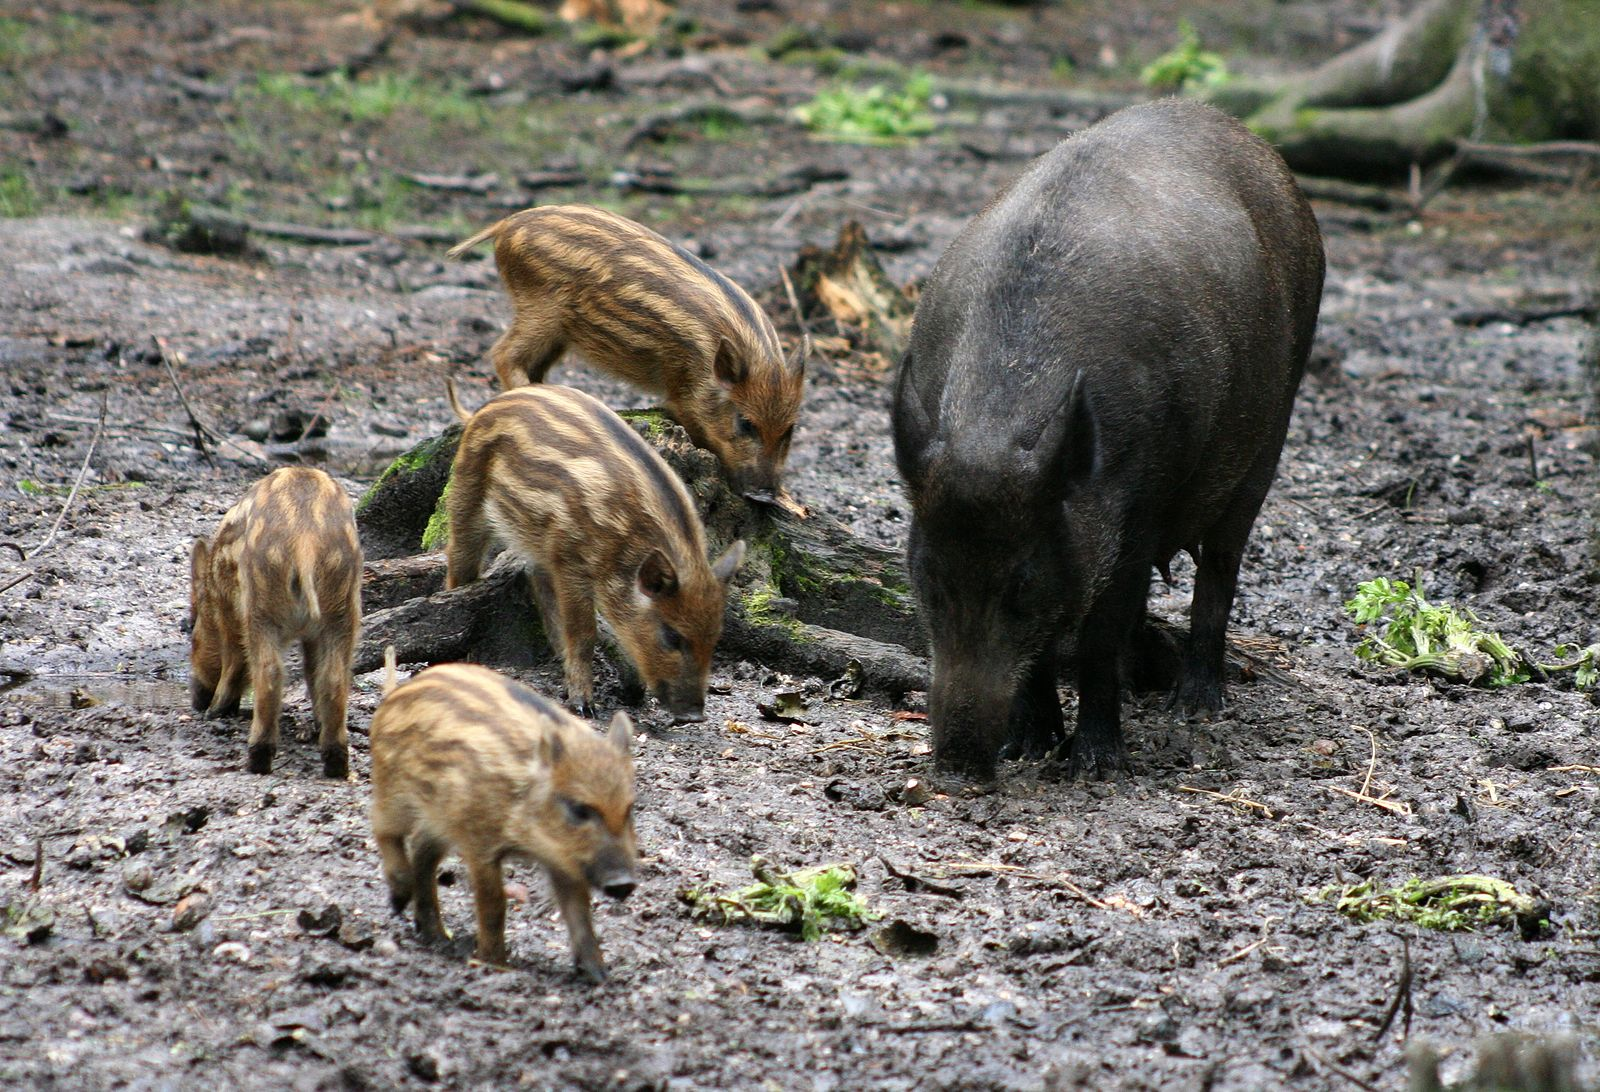
\includegraphics[width=0.6\linewidth]{Villsvin} \caption{Wild boar (*Sus scrofa*). Photo: Dave Pape}\label{fig:fig6}
\end{figure}

As an example of a study using a Lefkovitch matrix, we can consider the model of \citet{Bieber1} for female wild boar. Their model has annual time steps and three stages: Juveniles (age 0-1), yearlings (age 1-2) and adults (age 2+). Thus, the first to stages represent age classes lasting 1 year each, while the final stage contain all individuals of age 2 and above. Wild boar start reproducing before their first year, so in this case even the juveniles can contribute offspring to the next year's population (figure \ref{fig:wildboar}).

\begin{figure}
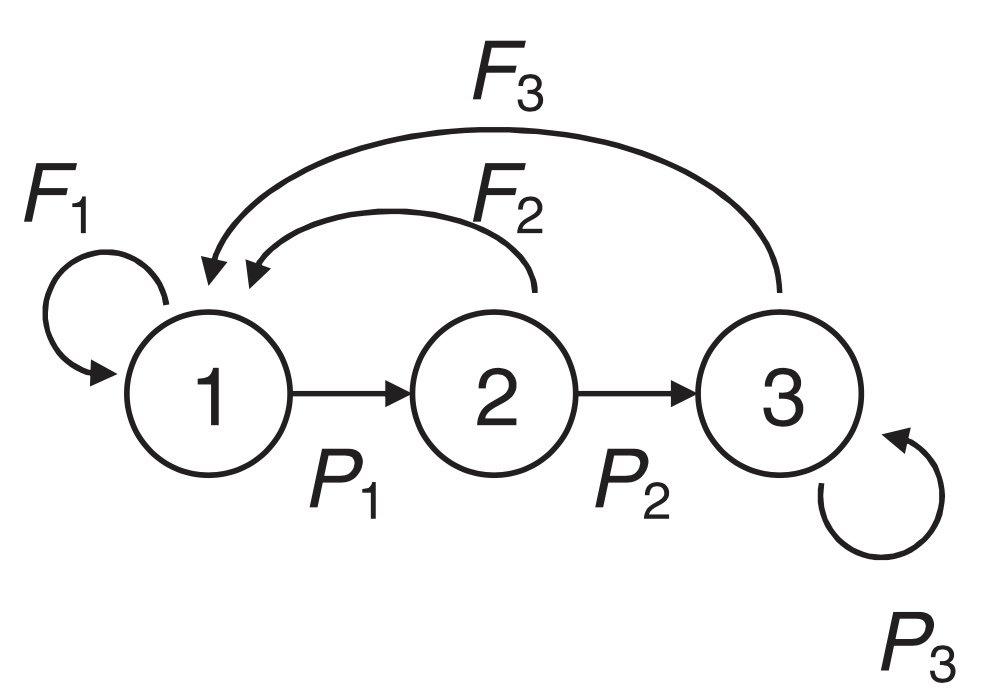
\includegraphics[width=0.6\linewidth]{LifeCycleBoar} \caption{Life cycle graph for the wild boar (*Sus scrofa*), fig 1 from @Bieber1.}\label{fig:wildboar}
\end{figure}

The projection matrix for this wild boar model is given by

\[
\mathbf{A}=\left[\begin{matrix} 0.26 & 0.94 &1.93  \\ 0.33&0  &0  \\ 0&0.4  &0.66  \\  \end{matrix}\right].
\]

This matrix is quite similar to an age structured model (Leslie matrix), but with the exception that adults do not necessarily die after reaching age 2, but can continue to live so that the final stage contains all individuals of age 2 and more (2+).

\hypertarget{agestage}{%
\subsection{Age by stage models}\label{agestage}}

Individuals in a population will always differ in more than one way, and sometimes (depending on the study question as well as the species) we have to account for more than one state variable in order to adequately describe the life history. For instance, we may need to combine age and life cycle stage, if the age differences within each stage are large. Even if age does not have a large effect on survival and fecundity compared to stage, we often need to describe how model outputs (e.g.~sensitivities) change with age, for instance to compare with other age-structured models. Models that combine age and stage are able to handle a wide range of possible structures - and can be seen as a special case of the general stage structured model where each class is a combination of age and stage.

For instance, there are \(k\) age classes, and \(m\) stages, the new age by stage model will have \(\phi=k*m\) classes in total. From these classes we can define a new projection matrix of dimension \(\phi \times \phi\), which can be analysed using the same methods as before to find \(\lambda\) and other parameters. For a broad overview of this kind of matrix model, see \citet{Caswell19}.

\hypertarget{example-black-headed-gulls}{%
\subsubsection*{Example: Black-headed gulls}\label{example-black-headed-gulls}}
\addcontentsline{toc}{subsubsection}{Example: Black-headed gulls}

\begin{figure}
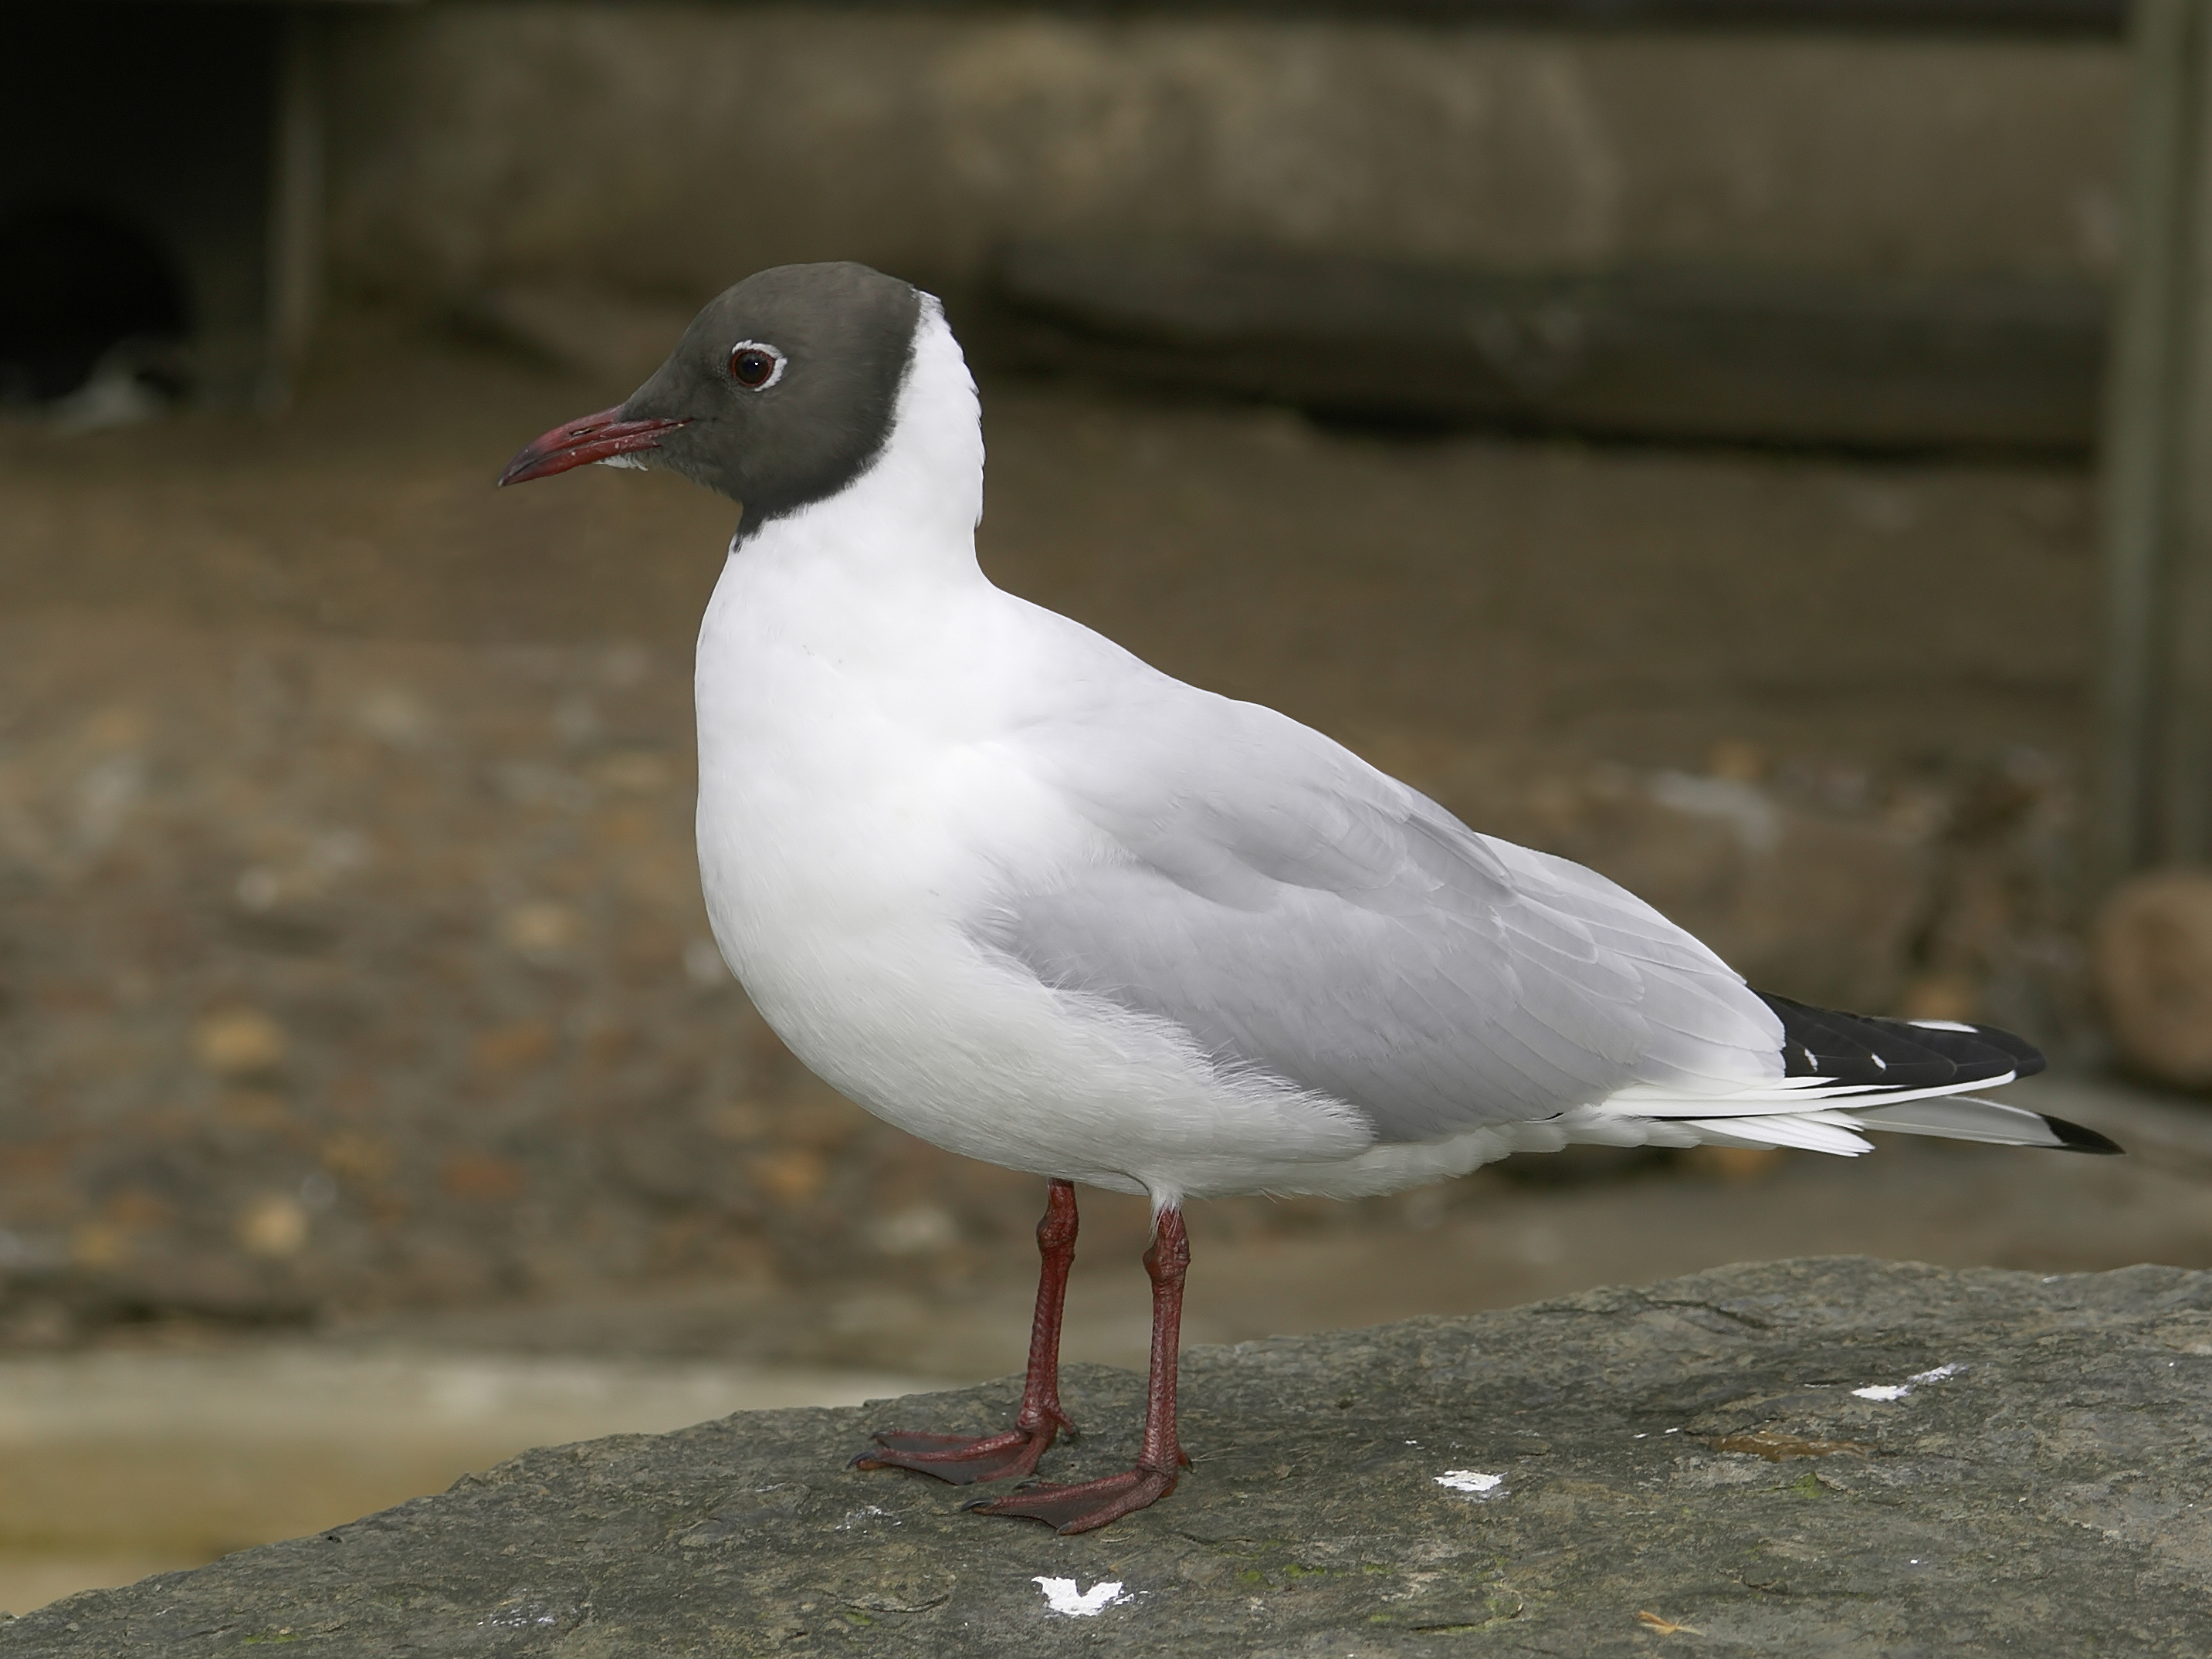
\includegraphics[width=0.6\linewidth]{BlackHeadedGull} \caption{Black-headed gull (*Chroicocephalus ridibundus*). Photo: Hans Hillewaert / [CC BY-SA 4.0](https://creativecommons.org/licenses/by-sa/4.0/)}\label{fig:BlackHeadedGull}
\end{figure}

\citet{Lebreton2} used an age-by-stage model to study a french colony of black-headed gulls (\emph{Chroicocephalus ridibundus}) living in two types of habitat of `good' and `poor' quality. In this species dispersal among habitats happens mainly before first reproduction, but young breeders may also disperse. \citet{Lebreton2} considered different scenarios for dispersal, here we will consider the scenario where only offspring disperse. This model was also used as an example by \citet{Hunter2} demonstrating a useful approach (`vec-permutation') to calculate sensitivity in age-by-stage models, and by \citet{Vindenes2020} in their introduction to matrix models.

The gulls have five main age classes corresponding to age 1, 2, 3, 4, and 5+ (all individuals of age 5 and older). With two habitats and five age classes we get a \(10\times 10\) projection matrix, where each stage corresponds to a combination of habitat and age class. There are two ways to structure such a matrix \citep{Lebreton2}: Either include age within habitat (so that the first five stages represent habitat 1 and the last five habitat 2), or habit within age class (the first two stages represent habitat 1 and 2 in age class 1, etc).

Using a structure of age within habitat, we get the following projection matrix \citep{Vindenes2020}:

\begin{align}\label{AGulls}
\mathbf{A}
&=\left[\begin{array}{ccccc|ccccc}
f_1&f_2&f_3&f_4&f_5 &0&0&0&0&0 \\
(1-p)s_1&0&0&0&0&qs_6&0&0&0&0\\
0&s_2&0&0&0&0&0&0&0&0\\
0&0&s_3&0&0&0&0&0&0&0\\
0&0&0&s_4&s_5&0&0&0&0&0\\
\hline
0&0&0&0&0&f_6&f_7&f_8&f_9&f_{10}\\
ps_1&0&0&0&0&(1-q)s_6&0&0&0&0\\
0&0&0&0&0&0&s_7&0&0&0\\
0&0&0&0&0&0&0&s_8&0&0\\
0&0&0&0&0&0&0&0&s_9&s_{10}\\
\end{array}\right].
\end{align}

The constants \(p\) and \(q\) describe dispersal probabilities of 1-year olds: The probability of dispersing from a good to a poor quality habitat is \(p\), while \(q\) is the probability of dispersing from the poor to the good habitat. This is also an example of source-sink dynamics, where the good habitat (the source) is sustaining the population living in the poor habitat (a sink). There is a limited number available number of breeding spots in good habitats, so some individuals are forced to use a lower quality site.

The survival coefficients are given by \(\mathbf{s}=[0.8, 0.82, 0.82, 0.82, 0.82]\) for both sites, while the fertility coefficients differ. In the good site they are given by \(\mathbf{f}_\text{good}=[0, 0.096, 0.16, 0.224, 0.32]\), and in the poor site by \(\mathbf{f}_{\text{poor}}=[0, 0.1, 0.16, 0.2, 0.2]\). Thus, for the youngest breeders the fertility is slightly higher in the poor site, but for older breeders the fertility is higher in the good site.

In R we can construct the projection matrix as a function of the dispersal rates \(p\) and \(q\) as follows:

\begin{Shaded}
\begin{Highlighting}[]
\NormalTok{Sboth }\OtherTok{\textless{}{-}} \FunctionTok{c}\NormalTok{(.}\DecValTok{8}\NormalTok{, }\FunctionTok{rep}\NormalTok{(.}\DecValTok{82}\NormalTok{,}\DecValTok{4}\NormalTok{))}
\NormalTok{Fgood }\OtherTok{\textless{}{-}} \FunctionTok{c}\NormalTok{(}\DecValTok{0}\NormalTok{, }\FloatTok{0.096}\NormalTok{, }\FloatTok{0.16}\NormalTok{, }\FloatTok{0.224}\NormalTok{, }\FloatTok{0.32}\NormalTok{) }
\NormalTok{Fpoor }\OtherTok{\textless{}{-}} \FunctionTok{c}\NormalTok{(}\DecValTok{0}\NormalTok{, }\FloatTok{0.1}\NormalTok{, }\FloatTok{0.16}\NormalTok{, }\FloatTok{0.2}\NormalTok{, }\FloatTok{0.2}\NormalTok{) }

\NormalTok{AmatGulls }\OtherTok{\textless{}{-}} \ControlFlowTok{function}\NormalTok{(p, q)\{}
\NormalTok{  SGood }\OtherTok{\textless{}{-}} \FunctionTok{c}\NormalTok{((}\DecValTok{1}\SpecialCharTok{{-}}\NormalTok{p)}\SpecialCharTok{*}\NormalTok{Sboth[}\DecValTok{1}\NormalTok{], Sboth[}\DecValTok{2}\SpecialCharTok{:}\DecValTok{5}\NormalTok{])}\CommentTok{\#Survival in good environment}
\NormalTok{  SPoor }\OtherTok{\textless{}{-}} \FunctionTok{c}\NormalTok{((}\DecValTok{1}\SpecialCharTok{{-}}\NormalTok{q)}\SpecialCharTok{*}\NormalTok{Sboth[}\DecValTok{1}\NormalTok{], Sboth[}\DecValTok{2}\SpecialCharTok{:}\DecValTok{5}\NormalTok{])}\CommentTok{\#Survival in poor environment}
\NormalTok{  Amat }\OtherTok{\textless{}{-}} \FunctionTok{matrix}\NormalTok{(}\DecValTok{0}\NormalTok{, }\DecValTok{10}\NormalTok{, }\DecValTok{10}\NormalTok{) }
  \CommentTok{\#{-}{-}{-}{-}{-}{-}{-}{-}{-}{-}{-}{-}{-}{-}{-}{-}{-}{-}{-}{-}{-}{-}{-}{-}{-}{-}{-}{-}{-}{-}{-}{-}{-}{-}{-}{-}{-}{-}{-}{-}{-}{-}{-}{-}{-}{-}{-}}
\NormalTok{  Amat[}\DecValTok{1}\NormalTok{, }\DecValTok{1}\SpecialCharTok{:}\DecValTok{5}\NormalTok{] }\OtherTok{\textless{}{-}}\NormalTok{ Fgood }\CommentTok{\# Fertility in good site}
\NormalTok{  Amat[}\DecValTok{6}\NormalTok{, }\DecValTok{6}\SpecialCharTok{:}\DecValTok{10}\NormalTok{] }\OtherTok{\textless{}{-}}\NormalTok{ Fpoor }\CommentTok{\# Fertility in poor site}
  \CommentTok{\#{-}{-}{-}{-}{-}{-}{-}{-}{-}{-}{-}{-}{-}{-}{-}{-}{-}{-}{-}{-}{-}{-}{-}{-}{-}{-}{-}{-}{-}{-}{-}{-}{-}{-}{-}{-}{-}{-}{-}{-}{-}{-}{-}{-}{-}{-}{-}}
  \FunctionTok{diag}\NormalTok{(Amat[}\DecValTok{2}\SpecialCharTok{:}\DecValTok{5}\NormalTok{,}\DecValTok{1}\SpecialCharTok{:}\DecValTok{4}\NormalTok{]) }\OtherTok{\textless{}{-}}\NormalTok{ SGood[}\DecValTok{1}\SpecialCharTok{:}\DecValTok{4}\NormalTok{] }\CommentTok{\#Survive and remain good site}
\NormalTok{  Amat[}\DecValTok{5}\NormalTok{,}\DecValTok{5}\NormalTok{] }\OtherTok{\textless{}{-}}\NormalTok{ SGood[}\DecValTok{5}\NormalTok{] }\CommentTok{\#Last age class}
  \FunctionTok{diag}\NormalTok{(Amat[}\DecValTok{7}\SpecialCharTok{:}\DecValTok{10}\NormalTok{,}\DecValTok{6}\SpecialCharTok{:}\DecValTok{9}\NormalTok{]) }\OtherTok{\textless{}{-}}\NormalTok{ SPoor[}\DecValTok{1}\SpecialCharTok{:}\DecValTok{4}\NormalTok{] }\CommentTok{\#Survive and remain poor site}
\NormalTok{  Amat[}\DecValTok{10}\NormalTok{,}\DecValTok{10}\NormalTok{] }\OtherTok{\textless{}{-}}\NormalTok{ SPoor[}\DecValTok{5}\NormalTok{] }\CommentTok{\#Last age class}
  \CommentTok{\#{-}{-}{-}{-}{-}{-}{-}{-}{-}{-}{-}{-}{-}{-}{-}{-}{-}{-}{-}{-}{-}{-}{-}{-}{-}{-}{-}{-}{-}{-}{-}{-}{-}{-}{-}{-}{-}{-}{-}{-}{-}{-}{-}{-}{-}{-}{-}}
\NormalTok{  Amat[}\DecValTok{7}\NormalTok{,}\DecValTok{1}\NormalTok{] }\OtherTok{\textless{}{-}}\NormalTok{ p}\SpecialCharTok{*}\NormalTok{Sboth[}\DecValTok{1}\NormalTok{] }\CommentTok{\#Dispersal from good to poor}
\NormalTok{  Amat[}\DecValTok{2}\NormalTok{,}\DecValTok{6}\NormalTok{] }\OtherTok{\textless{}{-}}\NormalTok{ q}\SpecialCharTok{*}\NormalTok{Sboth[}\DecValTok{1}\NormalTok{] }\CommentTok{\#Dispersal from poor to good}
  \CommentTok{\#{-}{-}{-}{-}{-}{-}{-}{-}{-}{-}{-}{-}{-}{-}{-}{-}{-}{-}{-}{-}{-}{-}{-}{-}{-}{-}{-}{-}{-}{-}{-}{-}{-}{-}{-}{-}{-}{-}{-}{-}{-}{-}{-}{-}{-}{-}{-}}
\NormalTok{  Amat}
\NormalTok{\}}
\end{Highlighting}
\end{Shaded}

With this function we can make calculate \(\lambda\) for different combinations of the two dispersal probabilities and plot the result:

\begin{Shaded}
\begin{Highlighting}[]
\CommentTok{\#Sequences of p and values}
\NormalTok{pVec }\OtherTok{\textless{}{-}}  \FunctionTok{seq}\NormalTok{(}\DecValTok{0}\NormalTok{,}\DecValTok{1}\NormalTok{,.}\DecValTok{01}\NormalTok{)}
\NormalTok{qVec }\OtherTok{\textless{}{-}}  \FunctionTok{seq}\NormalTok{(}\DecValTok{0}\NormalTok{,}\DecValTok{1}\NormalTok{,.}\DecValTok{01}\NormalTok{)}

\CommentTok{\#The expand\_grid function is useful for making new data frames for combinations of variables:}

\NormalTok{gulls\_table }\OtherTok{\textless{}{-}} \FunctionTok{expand\_grid}\NormalTok{(}\StringTok{"p"}\OtherTok{=}\NormalTok{pVec, }\StringTok{"q"}\OtherTok{=}\NormalTok{qVec )}

\NormalTok{lambdagulls }\OtherTok{\textless{}{-}} \ControlFlowTok{function}\NormalTok{(p, q)\{}
  \FunctionTok{uvlambda}\NormalTok{(}\FunctionTok{AmatGulls}\NormalTok{(}\AttributeTok{p=}\NormalTok{p,}\AttributeTok{q=}\NormalTok{q))}\SpecialCharTok{$}\NormalTok{lam}
\NormalTok{\}}

 
\NormalTok{gulls\_table }\OtherTok{\textless{}{-}}\NormalTok{ gulls\_table }\SpecialCharTok{\%\textgreater{}\%} \FunctionTok{rowwise}\NormalTok{() }\SpecialCharTok{\%\textgreater{}\%} \FunctionTok{mutate}\NormalTok{(}\AttributeTok{lambda=}\FunctionTok{lambdagulls}\NormalTok{(p,q))  }

\FunctionTok{ggplot}\NormalTok{(gulls\_table, }\FunctionTok{aes}\NormalTok{(}\AttributeTok{x=}\NormalTok{p, }\AttributeTok{y=}\NormalTok{q, }\AttributeTok{fill=}\NormalTok{lambda) ) }\SpecialCharTok{+} 
  \FunctionTok{geom\_tile}\NormalTok{()}\SpecialCharTok{+}
  \FunctionTok{scale\_fill\_viridis\_c}\NormalTok{()  }\SpecialCharTok{+}
  \FunctionTok{theme\_classic}\NormalTok{()}\SpecialCharTok{+}
  \FunctionTok{labs}\NormalTok{(}\AttributeTok{fill=}\FunctionTok{expression}\NormalTok{(lambda))}\SpecialCharTok{+}
    \FunctionTok{theme}\NormalTok{(}\AttributeTok{legend.position =} \StringTok{"top"}\NormalTok{ ) }\CommentTok{\#Place legend on top}
\end{Highlighting}
\end{Shaded}

\begin{figure}
\centering
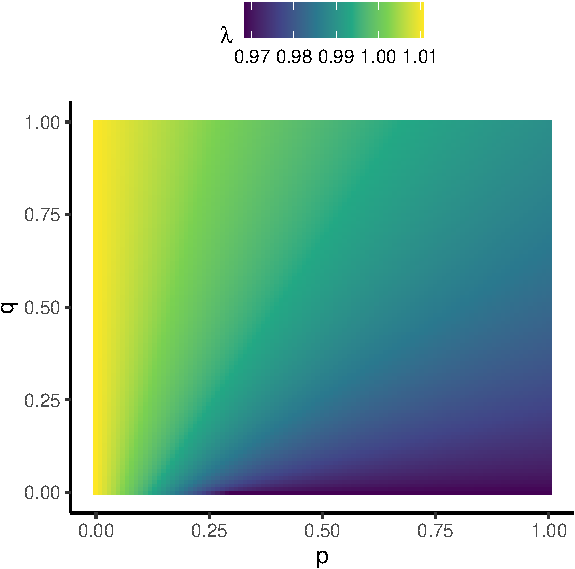
\includegraphics{DemographyCompendium_files/figure-latex/gullfig-1.pdf}
\caption{\label{fig:gullfig}Surface of \(\lambda\) as a function of dispersal parameters \(p\) (probability of leaving the `good' site) and \(q\) (probability of leaving the `poor' site) in the black-headed gull model.}
\end{figure}

\hypertarget{disease-models}{%
\subsection{Disease models}\label{disease-models}}

Stage structured matrix model play an important role in understanding disease dynamics, for systems that can be analysed with discrete time models. Classifying host individuals according to disease status (susceptible, infected, etc) is essential, and often other sources of variation need to be accounted for as well (age, sex, and other factors that can affect disease transmission and immunity). Space is another fundamental factor that often needs to be included to accurately capture the dynamics of an epidemic. In host-vector-pathogen systems the vector can also be classified according to multiple stages.

Disease dynamics are inherently frequency-dependent, so cannot be analyzed with the density independent methods presented so far, but they often have equilibrium dynamics that are analysed with matrix model methods. The parameter \(R_0\) (that we now know as the lifetime reproductive success) has an important interpretation in disease models as the total number of new infections that each infected individual will give rise to in a susceptible population. In other words it is the lifetime reproductive success of the pathogen.

One of the simplest and most common models for disease dynamics is the SIR model \citep{Kermack1}, classifying host individuals into three disease states (Susceptible - Infected - Recovered). This is an example of a compartmental model in epidemiology.

\hypertarget{integral-projection-models-ipms}{%
\section{Integral projection models (IPMs)}\label{integral-projection-models-ipms}}

Many state variables are intrinsically continuous, such as body size. Matrix models can still be used to study size structure by lumping individuals into different discrete size classes, but this adds an extra modeling decision of where to set the limits for each size class. And sometimes this decision affects the results of the model. This can be avoided by using an IPM, i.e.~an \textbf{integral projection model} \citep{Easterling1}, which accomodates continuous state variables. Instead of a population vector with a discrete number of stages, IPMs track individuals over a continuous trait distribution \(n(z)\), where \(z\) represents the trait measure (e.g.~size), and instead of a projection matrix, IPMs use a projection kernel. You can think of an IPM as a matrix model with infinitely many stages, and in fact they belong to the same class of models (matrix models). The good news is that IPMs can be analysed with matrix model methods (e.g.~those introduced in chapter \ref{s03-MatrixModels}) to find \(\lambda\) and other model outputs. In R, we then specify the mesh size of the kernel (creating a matrix), and the finer the mesh size the more accurate are the estimated model outputs.

IPMs and matrix models are both part of the same model framework (matrix models). The main difference between an IPM and a matrix model is in how the underlying parameters are (typically) estimated from data: With IPMs we typically use some kind of regression model, where the state variable is an explanatory variable explaining the survival, fecundity and transition rates that define the model. With matrix models, these parameters are usually estimated independently within each stage, without treating the stage as an explanatory variable - however regression models can still be used to estimate parameters of a matrix model. We will not go into details regarding IPMs here, but you have already learned the methods for analyzing them, as they are the same as for matrix models. For more details on IPMs and their application, see \citet{Ellner5}.

\hypertarget{exercises-3}{%
\section{Exercises}\label{exercises-3}}

For suggested solutions, see appendix \ref{s09-Solutions}.

\hypertarget{exercise-4.1}{%
\subsection*{Exercise 4.1}\label{exercise-4.1}}
\addcontentsline{toc}{subsection}{Exercise 4.1}

\begin{enumerate}
\def\labelenumi{\arabic{enumi}.}
\tightlist
\item
  Draw the life cycle graph for each of the projection matrices below.
\end{enumerate}

\[\mathbf{A}=\left[\begin{matrix}0.5&2\\1&0.7\end{matrix}\right]\]

\[\mathbf{A}=\left[\begin{matrix}0&0&10\\0.9&0&0\\0&0.9&0\end{matrix}\right]\]

\[\mathbf{A}=\left[\begin{matrix}0&8&5\\0.9&0.1&0.7\\0&0.7&0.2\end{matrix}\right]\]

\begin{enumerate}
\def\labelenumi{\arabic{enumi}.}
\setcounter{enumi}{1}
\item
  Can you determine the stage-specific survival probability in each case? What assumption(s) do you need to make in order to do this?
\item
  What could the stages represent in each case?
\end{enumerate}

\hypertarget{exercise-4.2}{%
\subsection*{Exercise 4.2}\label{exercise-4.2}}
\addcontentsline{toc}{subsection}{Exercise 4.2}

This exercise is based on an experimental toxicology study by \citet{Kammenga1}, and their model for the isopod common woodlouse (\emph{Porcellio scaber}) was also used as an example by \citet{Vindenes2020}. The woodlouse model has seven discrete life history stages and monthly time steps.

\begin{figure}
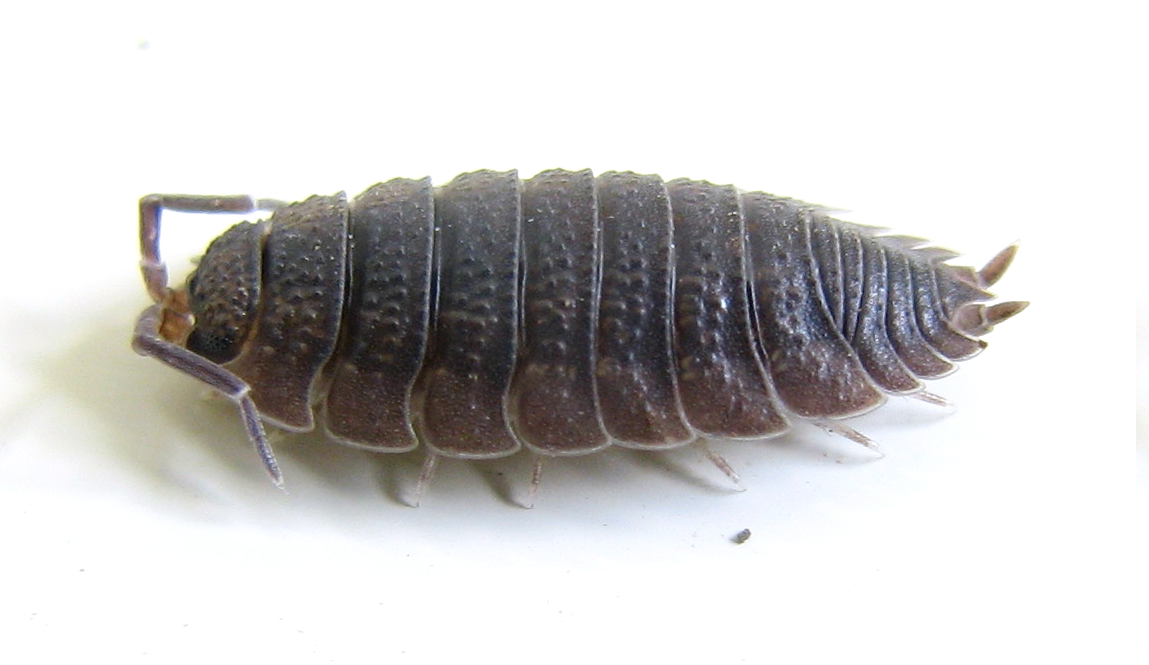
\includegraphics[width=0.4\linewidth]{Porcellio_scaber} \caption{Common woodlouse (*Porcellio scaber*). }\label{fig:Porcellio1}
\end{figure}

There are 7 main stages in this woodlouse model:

\begin{enumerate}
\def\labelenumi{\arabic{enumi}.}
\tightlist
\item
  Oocytes\\
\item
  Eggs/offspring (in marsupium)\\
\item
  Juveniles\\
\item
  First (spring) reproductive stage\\
\item
  Non-reproductive adult stage\\
\item
  Second (summer) reproductive stage\\
\item
  Senescent non-reproductive stage
\end{enumerate}

The following life cycle graph is from \citet{Kammenga1} (fig.~1):

\begin{figure}
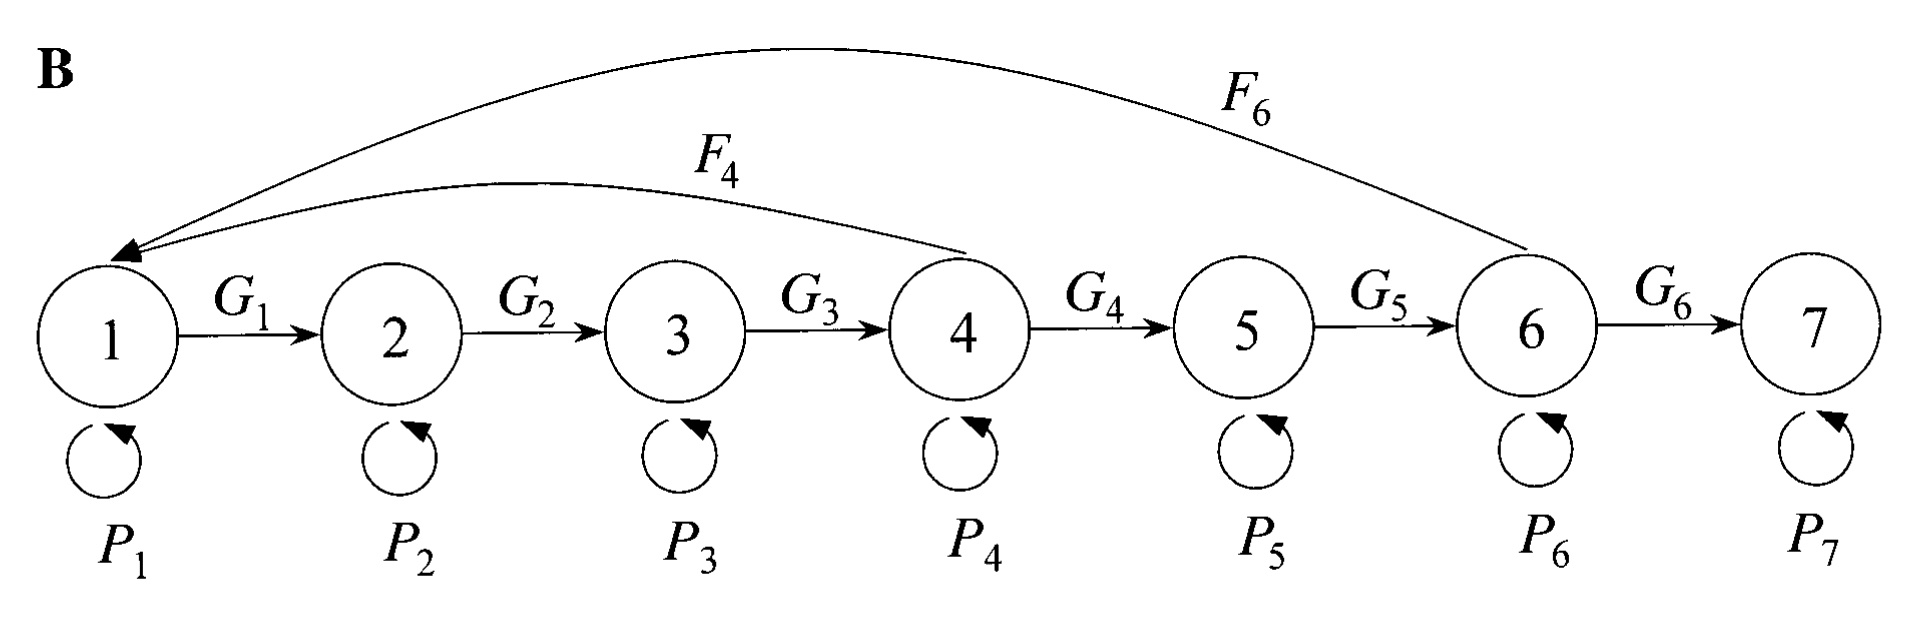
\includegraphics[width=0.8\linewidth]{Porcellio_scaber2} \caption{Life cycle graph for the common woodlouse (*Porcellio scaber*), fig 1B from @Kammenga1.}\label{fig:Porcellio2}
\end{figure}

The vectors of P, G and F in R have the following values:

\begin{tabular}{c|c|c|c}
\hline
Stage & P & G & F\\
\hline
1 & 0.158 & 0.722 & 0.000\\
\hline
2 & 0.545 & 0.245 & 0.000\\
\hline
3 & 0.539 & 0.231 & 0.000\\
\hline
4 & 0.162 & 0.788 & 2.355\\
\hline
5 & 0.008 & 0.792 & 0.000\\
\hline
6 & 0.136 & 0.664 & 5.568\\
\hline
7 & 0.800 & 0.000 & 0.000\\
\hline
\end{tabular}

\begin{enumerate}
\def\labelenumi{\arabic{enumi}.}
\item
  Use the life cycle graph and the vectors defined in the table to define the fertility matrix \(\mathbf{F}\), the survival matrix \(\mathbf{U}\), and the projection matrix \(\mathbf{A}\) in R.
\item
  Decompose the matrices \(\mathbf{U}\) and \(\mathbf{F}\) to calculate the stage-specific fertility and survival probability, and the transition matrix (based on the decomposition in equation \eqref{eq:General}. Plot the stage-specific fertility and survival probability.
\item
  Calculate \(\lambda\), the stable stage structure \(\mathbf{u}\) and reproductive values \(\mathbf{v}\), and plot \(\mathbf{u}\) and \(\mathbf{v}\). How fast does this population grow per year? Does this model work well to describe a life history that reproduces twice per year \citep{Kammenga1}?
\item
  Write an R function that returns the value of \(\lambda\) for this population for a set of three vectors corresponding to \emph{proportional changes} to elements of \(P\), \(G\) or \(F\). What happens to \(\lambda\), \(\mathbf{u}\) and \(\mathbf{v}\) if you modify the element \(G_6\) in the vector \(G\)? Explain why.
\item
  What happens to \(\lambda\), \(\mathbf{u}\) and \(\mathbf{v}\) if you modify the element \(G_4\)? Explain why.
\end{enumerate}

\hypertarget{exercise-4.3}{%
\subsection*{Exercise 4.3}\label{exercise-4.3}}
\addcontentsline{toc}{subsection}{Exercise 4.3}

This exercise will continue with the woodlouse model from the previous exercise.

\citet{Kammenga1} considered toxicological effects of cadmium. At the highest concentration, the woodlouse will switch to only one reproductive event instead of two, and the survival probabilities are reduced between 7 and 12 \% in all stages except the egg stage. In addition the development time of eggs decreased \citep{Kammenga1}. For this exercise we assume the values of \(P\), \(G\), and \(F\) corresponding to cadmium exposure are given by

\begin{tabular}{c|c|c|c}
\hline
Stage & P & G & F\\
\hline
1 & 0.158 & 0.722 & 0.000\\
\hline
2 & 0.491 & 0.220 & 0.000\\
\hline
3 & 0.485 & 0.208 & 0.000\\
\hline
4 & 0.145 & 0.710 & 2.355\\
\hline
5 & 0.007 & 0.713 & 0.000\\
\hline
6 & 0.122 & 0.598 & 0.000\\
\hline
7 & 0.720 & 0.000 & 0.000\\
\hline
\end{tabular}

\begin{enumerate}
\def\labelenumi{\arabic{enumi}.}
\item
  Define a new matrix \(\mathbf{A}_C\) (C for cadmium) in R based on these values. This is now a treatment matrix, while the previously defined matrix is the reference matrix.
\item
  Calculate \(\lambda\) for the new matrix. How does it compare to the previous value?
\item
  Calculate the halfway matrix \(\mathbf{A}^*\) and the difference matrix \(\mathbf{D}\).
\item
  Calculate the sensitivity matrix \(\mathbf{S}^*\) based on the halfway matrix, and finally calculate and plot the elements of the matrix corresponding to the contributions to the difference in \(\lambda\) between \(\mathbf{A}\) and \(\mathbf{A}_C\). Which element contributes the most?
\item
  Why is it often better to use an LTRE than a sensitivity analysis when we want to understand the impacts of an external factor such as a toxicant?
\end{enumerate}

\hypertarget{Stochasticity}{%
\chapter{Stochasticity}\label{Stochasticity}}

This chapter will give an introduction to stochastic environments and bet-hedging strategies. The underlying theory is based on stochastic processes and probability theory, and this chapter will only touch upon a few basic concepts from this large research field. A key result from the most basic model of stochastic population growth is that the long-term population growth rate (fitness) in variable environments will always be lower than the growth rate in the constant mean environment.

\hypertarget{learning-goals-4}{%
\section{Learning goals}\label{learning-goals-4}}

\begin{itemize}
\item
  Understand key properties of population growth in variable environments.
\item
  Describe the main properties of the Lewontin-Cohen model.
\item
  Understand how bet-hedging strategies can help individuals live in variable environments.
\item
  Discuss the role of variable and unpredictable environments in light of climate change.
\end{itemize}

\hypertarget{variable-vs-unpredictable-environments}{%
\section{Variable vs unpredictable environments}\label{variable-vs-unpredictable-environments}}

So far we have only considered populations in constant environments. But natural environments can be highly variable, both in time and space. Here, `environment' is a very general term which can refer to any particular abiotic variable (like temperature) or a combination of several factors that affect organisms living in the habitat, including biotic factors like resource availability. Environmental variability can be \emph{predictable}, like the seasonal changes in light conditions at high latitudes, or \emph{unpredictable} - which is the case for stochastic environments. Unpredictable variation also includes rare events such as rainfalls in a dessert, or flooding and wildfires. We can estimate a frequency at which such events typically occur over many years, but it is difficult to predict the exact timing of each such event.

Practically all organisms live in some kind of variable environment (although some habitats are more stable than others, for instance the deep depths of the oceans), and species have evolved various strategies to deal with both the wide range of possible conditions they (or their offspring) may encounter, under varying degrees of predictability. These adaptations allow individuals to mitigate negative impacts of bad conditions, as well as take advantage of good conditions, and spread the risk associated with uncertainty in various ways.

If the environment is fluctuating in a predictable way, \textbf{phenotypic plasticity} can allow individuals to cope with the variation. Organisms can then take advantage of environmental cues during development to achieve an optimum phenotype in the future environment. For unpredictable (stochastic) environments, however, organisms cannot rely on such cues. In these cases \textbf{bet-hedging} strategies may evolve.

\hypertarget{the-lewontin-cohen-model}{%
\section{The Lewontin-Cohen model}\label{the-lewontin-cohen-model}}

The simplest model for stochastic population growth applies to an unstructured population. In this model the annual population growth rate is a stochastic variable \(\Lambda_t\) with mean \(\text{E}[\Lambda_t]=\lambda\), variance \(\text{Var}(\Lambda)=\sigma^2\), and with no autocorrelation between the growth rates of different years. This means that the annual growth rates are IID (Identically and Independently Distributed), and this assumption is important for the derivation of the long-term population growth rate. This model is the Lewontin-Cohen model \citep{Lewontin1}, also known as a `geometric random walk'.

\hypertarget{defining-the-process}{%
\subsection{Defining the process}\label{defining-the-process}}

Starting from a population size \(N_0\), the population size after \(t\) time steps in the Lewontin-Cohen model is given by

\begin{align} 
N_{t+1}=\Lambda_{t}\Lambda_{t-1}\cdots\Lambda_{1}\Lambda_0N_0=N_0\prod_{i=0}^t \Lambda_i.
\label{eq:Lewontin1}
\end{align}
We are interested in the behavior of a `typical' population growing according to this process, and to define the long-term growth rate of such a `typical' population (the socalled stochastic growth rate). As we will see below, this is not the growth rate of the mean population size, but rather the median population size. Before we go into details of this derivation, we will look at how we can generate realizations of the Lewontin-Cohen process in R and plot one or more realizations.

\hypertarget{plot-one-realization-of-the-process}{%
\subsubsection*{Plot one realization of the process}\label{plot-one-realization-of-the-process}}
\addcontentsline{toc}{subsubsection}{Plot one realization of the process}

The R function \texttt{LC} below can be used to generate a random sequence of population sizes over time based on this model (each time you run the code it will generate a different sequence, unless you use the function \texttt{set.seed()} which initializes the pseudorandom number generator in R). The \texttt{LC} function returns the sequence of population sizes as a data frame, including the time steps from 0 to the set number of years. The output from one run of the function is shown in figure \ref{fig:Lewontin}. In this example, a normal distribution is used to generate the sequence of annual growth rates, but the exact kind of distribution is not critical as long as the mean and variance can be set independently (for instance, a lognormal distribution could be used since all the multiplicative growth rates should be non-negative).

\begin{Shaded}
\begin{Highlighting}[]
\CommentTok{\#mean.lambda: Expectation of annual lambda}
\CommentTok{\#sd.lambda: Standard deviation of lambda}

\NormalTok{LC }\OtherTok{\textless{}{-}} \ControlFlowTok{function}\NormalTok{(}\AttributeTok{Tmax=}\DecValTok{30}\NormalTok{, }\AttributeTok{n0=}\DecValTok{100}\NormalTok{, }\AttributeTok{mean.lambda=}\FloatTok{1.05}\NormalTok{, }\AttributeTok{sd.lambda=}\FloatTok{0.1}\NormalTok{)\{}
\NormalTok{  stochastic.lambdas }\OtherTok{\textless{}{-}} \FunctionTok{rnorm}\NormalTok{(Tmax, }\AttributeTok{mean=}\NormalTok{mean.lambda, }\AttributeTok{sd=}\NormalTok{sd.lambda)}
\NormalTok{  Nvec }\OtherTok{\textless{}{-}} \FunctionTok{rep}\NormalTok{(}\ConstantTok{NA}\NormalTok{, Tmax}\SpecialCharTok{+}\DecValTok{1}\NormalTok{)}
\NormalTok{  Nvec[}\DecValTok{1}\NormalTok{] }\OtherTok{\textless{}{-}}\NormalTok{ n0}
  \ControlFlowTok{for}\NormalTok{(i }\ControlFlowTok{in} \DecValTok{1}\SpecialCharTok{:}\NormalTok{Tmax)\{}
\NormalTok{    Nvec[i}\SpecialCharTok{+}\DecValTok{1}\NormalTok{] }\OtherTok{\textless{}{-}}\NormalTok{ stochastic.lambdas[i]}\SpecialCharTok{*}\NormalTok{Nvec[i]}
\NormalTok{  \}}
  \FunctionTok{data.frame}\NormalTok{(}\StringTok{"Time"}\OtherTok{=}\DecValTok{0}\SpecialCharTok{:}\NormalTok{Tmax, }\StringTok{"N"}\OtherTok{=}\NormalTok{Nvec)}
\NormalTok{\}}

\FunctionTok{set.seed}\NormalTok{(}\DecValTok{20}\NormalTok{) }\CommentTok{\#Initialize R\textquotesingle{}s random number generator (keep to get reproducible results, remove to get a new sequence each time)}

\CommentTok{\#Apply function and plot result:}
\NormalTok{StochasticGrowth }\OtherTok{\textless{}{-}} \FunctionTok{LC}\NormalTok{()}

\FunctionTok{ggplot}\NormalTok{(StochasticGrowth) }\SpecialCharTok{+} 
  \FunctionTok{geom\_line}\NormalTok{(}\FunctionTok{aes}\NormalTok{(}\AttributeTok{x=}\NormalTok{Time, }\AttributeTok{y=}\NormalTok{N), }\AttributeTok{lwd=}\FloatTok{1.2}\NormalTok{)}\SpecialCharTok{+}
  \FunctionTok{geom\_point}\NormalTok{(}\FunctionTok{aes}\NormalTok{(}\AttributeTok{x=}\NormalTok{Time, }\AttributeTok{y=}\NormalTok{N), }\AttributeTok{size=}\DecValTok{3}\NormalTok{)}\SpecialCharTok{+}
  \FunctionTok{theme\_bw}\NormalTok{() }\SpecialCharTok{+}
  \FunctionTok{labs}\NormalTok{( }\AttributeTok{x=}\StringTok{"Time (year)"}\NormalTok{, }\AttributeTok{y=}\StringTok{"Population size N"}\NormalTok{)  }
\end{Highlighting}
\end{Shaded}

\begin{figure}
\centering
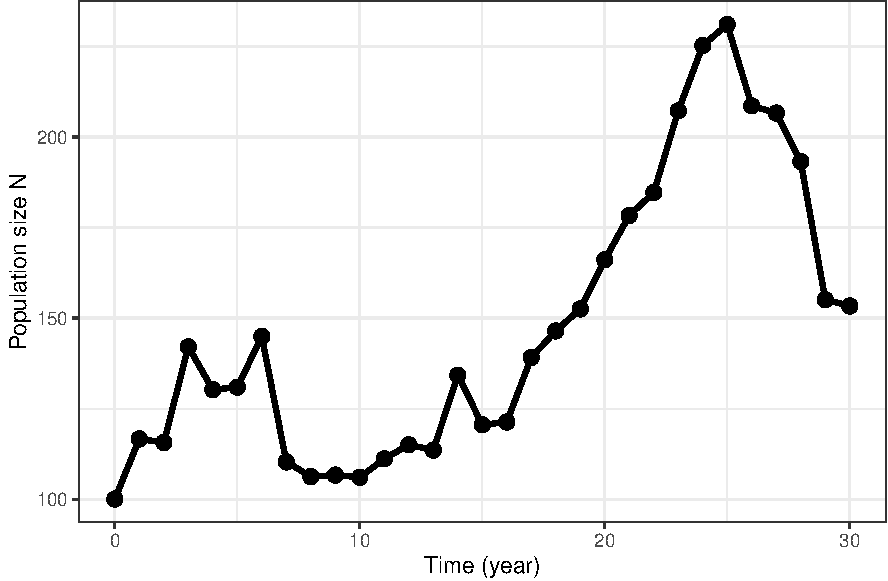
\includegraphics{DemographyCompendium_files/figure-latex/Lewontin-1.pdf}
\caption{\label{fig:Lewontin}Stochastic population growth following the Lewontin-Cohen model with normally distributed annual growth rates with mean \(\lambda=1.05\) and standard deviation \(\sigma=.1\)}
\end{figure}

This code only generates one realization of the growth process. To learn more about the typical behavior of this stochastic growth process we need to generate many realizations (from the same starting point, with the same mean and variance of the annual growth rate) and look at some summary statistics.

\hypertarget{plot-many-realizations-of-the-process}{%
\subsubsection*{Plot many realizations of the process}\label{plot-many-realizations-of-the-process}}
\addcontentsline{toc}{subsubsection}{Plot many realizations of the process}

The following function generates a chosen number (\texttt{nsim}) of realizations of the Lewontin-Cohen model, stores them in a data frame and makes a plot of all of them.

\begin{Shaded}
\begin{Highlighting}[]
\NormalTok{nsimLC }\OtherTok{\textless{}{-}} \ControlFlowTok{function}\NormalTok{(}\AttributeTok{nsim=}\DecValTok{100}\NormalTok{, }\AttributeTok{Tmax=}\DecValTok{30}\NormalTok{, }\AttributeTok{n0=}\DecValTok{100}\NormalTok{, }\AttributeTok{mean.lambda=}\FloatTok{1.05}\NormalTok{, }\AttributeTok{sd.lambda=}\FloatTok{0.1}\NormalTok{)\{}
\NormalTok{  frame }\OtherTok{\textless{}{-}}  \FunctionTok{data.frame}\NormalTok{(}\StringTok{"Time"}\OtherTok{=}\DecValTok{0}\SpecialCharTok{:}\NormalTok{Tmax)}
  \ControlFlowTok{for}\NormalTok{(j }\ControlFlowTok{in} \DecValTok{1}\SpecialCharTok{:}\NormalTok{nsim)\{}
\NormalTok{  stochastic.lambdas }\OtherTok{\textless{}{-}} \FunctionTok{rnorm}\NormalTok{(Tmax, }\AttributeTok{mean=}\NormalTok{mean.lambda, }\AttributeTok{sd=}\NormalTok{sd.lambda)}
\NormalTok{  Nvec }\OtherTok{\textless{}{-}} \FunctionTok{rep}\NormalTok{(}\ConstantTok{NA}\NormalTok{, Tmax}\SpecialCharTok{+}\DecValTok{1}\NormalTok{)}
\NormalTok{  Nvec[}\DecValTok{1}\NormalTok{] }\OtherTok{\textless{}{-}}\NormalTok{ n0}
  \ControlFlowTok{for}\NormalTok{(i }\ControlFlowTok{in} \DecValTok{1}\SpecialCharTok{:}\NormalTok{Tmax)\{}
\NormalTok{    Nvec[i}\SpecialCharTok{+}\DecValTok{1}\NormalTok{] }\OtherTok{\textless{}{-}}\NormalTok{ stochastic.lambdas[i]}\SpecialCharTok{*}\NormalTok{Nvec[i]}
\NormalTok{  \}}
\NormalTok{  frame }\OtherTok{\textless{}{-}} \FunctionTok{cbind}\NormalTok{(frame, Nvec)}
  \FunctionTok{names}\NormalTok{(frame)[j}\SpecialCharTok{+}\DecValTok{1}\NormalTok{] }\OtherTok{\textless{}{-}} \FunctionTok{paste}\NormalTok{(}\StringTok{"N"}\NormalTok{,j,}\AttributeTok{sep=}\StringTok{""}\NormalTok{)}
\NormalTok{  \}}
\NormalTok{  frame}
\NormalTok{\}}
\end{Highlighting}
\end{Shaded}

To apply this function and plot the results, we can use the following code:

\begin{Shaded}
\begin{Highlighting}[]
\FunctionTok{set.seed}\NormalTok{(}\DecValTok{20}\NormalTok{) }

\NormalTok{simLC100 }\OtherTok{\textless{}{-}} \FunctionTok{nsimLC}\NormalTok{()}

\NormalTok{simLC100.long }\OtherTok{\textless{}{-}}\NormalTok{ simLC100 }\SpecialCharTok{\%\textgreater{}\%} \FunctionTok{pivot\_longer}\NormalTok{(}\FunctionTok{c}\NormalTok{(}\SpecialCharTok{{-}}\NormalTok{Time),}
               \AttributeTok{names\_to =} \StringTok{"Rep"}\NormalTok{, }\AttributeTok{values\_to =} \StringTok{"N"}\NormalTok{)}

\FunctionTok{ggplot}\NormalTok{(simLC100.long) }\SpecialCharTok{+} 
  \FunctionTok{geom\_line}\NormalTok{(}\FunctionTok{aes}\NormalTok{(}\AttributeTok{x=}\NormalTok{Time, }\AttributeTok{y=}\NormalTok{N, }\AttributeTok{col=}\NormalTok{Rep), }\AttributeTok{lwd=}\NormalTok{.}\DecValTok{5}\NormalTok{)}\SpecialCharTok{+}
  \FunctionTok{scale\_color\_manual}\NormalTok{(}\AttributeTok{values=}\FunctionTok{rep}\NormalTok{(}\DecValTok{1}\NormalTok{,}\DecValTok{100}\NormalTok{))}\SpecialCharTok{+}
  \FunctionTok{theme\_bw}\NormalTok{() }\SpecialCharTok{+}
   \FunctionTok{theme}\NormalTok{(}\AttributeTok{legend.position =} \StringTok{"none"}\NormalTok{ )}\SpecialCharTok{+}
  \FunctionTok{labs}\NormalTok{( }\AttributeTok{x=}\StringTok{"Time (year)"}\NormalTok{, }\AttributeTok{y=}\StringTok{"Population size N"}\NormalTok{)  }
\end{Highlighting}
\end{Shaded}

\begin{figure}
\centering
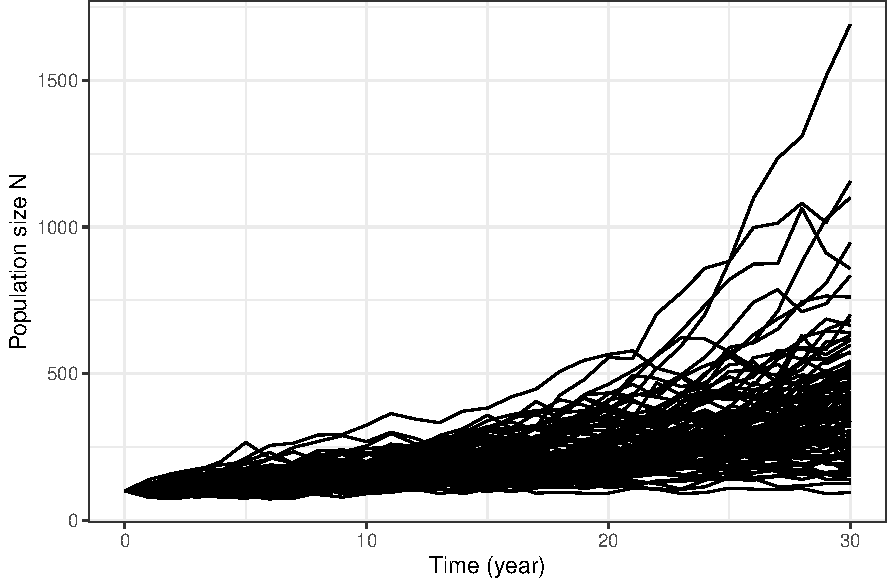
\includegraphics{DemographyCompendium_files/figure-latex/Lewontin2-1.pdf}
\caption{\label{fig:Lewontin2}100 realizations of the Lewontin-Cohen model with normally distributed annual growth rates, with mean \(\lambda=1.05\) and standard deviation \(\sigma=.1\)}
\end{figure}

Figure \ref{fig:Lewontin2} shows the output from 100 realizations. We see that over time, these realizations diverge more and more from each other as the randomness accumulates. A few realizations reach large population sizes, while many are located in intermediate values. However, it quickly gets quite messy to plot so many realizations, and if we want more than 100 it will be even worse. If we want to summarize the outcome of many realizations over time, a better option is to plot selected \textbf{percentiles} over time.

\hypertarget{plot-percentiles-from-many-realizations}{%
\subsubsection*{Plot percentiles from many realizations}\label{plot-percentiles-from-many-realizations}}
\addcontentsline{toc}{subsubsection}{Plot percentiles from many realizations}

Percentiles (or quantiles) are useful for summarizing outputs from many realizations. For instance, the 50\%\%\% percentile represents the population size at which 50\(\%\) of the realizations will lie above it and 50\(\%\) below it (i.e.~the median in the limit as the number of realizations approaches infinty), the 95\(\%\) percentile represents the population size at which 5\(\%\) of the realizations lies above it and 5\(\%\) below it, etc. The following code makes such a plot based on 10 000 realizations of the Lewontin-Cohen process. It can take some seconds to run (reduce the number of realizations \texttt{nsim} if it gets too slow)

\begin{Shaded}
\begin{Highlighting}[]
\CommentTok{\#Apply function to get 10 0000 realizations (can take some time)}
\NormalTok{simLC\_Large }\OtherTok{\textless{}{-}} \FunctionTok{nsimLC}\NormalTok{(}\AttributeTok{nsim=}\DecValTok{10000}\NormalTok{)}

\CommentTok{\#Get the 5, 25, 50, 75, and 95 percentiles:}
\NormalTok{Percentiles1  }\OtherTok{\textless{}{-}} \FunctionTok{t}\NormalTok{(}\FunctionTok{apply}\NormalTok{(}\FunctionTok{t}\NormalTok{(simLC\_Large[,}\SpecialCharTok{{-}}\DecValTok{1}\NormalTok{]),}\DecValTok{2}\NormalTok{, quantile, }\AttributeTok{probs=}\FunctionTok{c}\NormalTok{(.}\DecValTok{05}\NormalTok{, .}\DecValTok{25}\NormalTok{, .}\DecValTok{5}\NormalTok{, .}\DecValTok{75}\NormalTok{,.}\DecValTok{95}\NormalTok{)))}

 
\CommentTok{\#Store percentiles in data frame  }
\NormalTok{LCPercentiles }\OtherTok{\textless{}{-}} \FunctionTok{as.data.frame}\NormalTok{(}\FunctionTok{cbind}\NormalTok{(}\StringTok{"Time"}\OtherTok{=}\DecValTok{0}\SpecialCharTok{:}\NormalTok{(}\FunctionTok{dim}\NormalTok{(Percentiles1)[}\DecValTok{1}\NormalTok{]}\SpecialCharTok{{-}}\DecValTok{1}\NormalTok{), Percentiles1))}

\NormalTok{LCPercentiles}\SpecialCharTok{$}\NormalTok{Mean }\OtherTok{\textless{}{-}} \FunctionTok{apply}\NormalTok{(}\FunctionTok{t}\NormalTok{(simLC\_Large[,}\SpecialCharTok{{-}}\DecValTok{1}\NormalTok{]),}\DecValTok{2}\NormalTok{, mean)}


\CommentTok{\#Make long format for plotting}
\NormalTok{LCPercentiles.long }\OtherTok{\textless{}{-}}\NormalTok{ LCPercentiles }\SpecialCharTok{\%\textgreater{}\%} \FunctionTok{pivot\_longer}\NormalTok{(}\FunctionTok{c}\NormalTok{(}\SpecialCharTok{{-}}\NormalTok{Time),}
               \AttributeTok{names\_to =} \StringTok{"Percentile"}\NormalTok{, }\AttributeTok{values\_to =} \StringTok{"N"}\NormalTok{)}

\CommentTok{\#Make sure the order of the percentiles is correct}
\NormalTok{LCPercentiles.long}\SpecialCharTok{$}\NormalTok{Percentile }\OtherTok{\textless{}{-}} \FunctionTok{factor}\NormalTok{(LCPercentiles.long}\SpecialCharTok{$}\NormalTok{Percentile, }\AttributeTok{levels=}\FunctionTok{c}\NormalTok{(}\StringTok{"5\%"}\NormalTok{, }\StringTok{"25\%"}\NormalTok{, }\StringTok{"50\%"}\NormalTok{, }\StringTok{"75\%"}\NormalTok{, }\StringTok{"95\%"}\NormalTok{,}\StringTok{"Mean"}\NormalTok{))}

\FunctionTok{ggplot}\NormalTok{(LCPercentiles.long) }\SpecialCharTok{+} 
  \FunctionTok{geom\_line}\NormalTok{(}\FunctionTok{aes}\NormalTok{(}\AttributeTok{x=}\NormalTok{Time, }\AttributeTok{y=}\NormalTok{N, }\AttributeTok{col=}\NormalTok{Percentile,}\AttributeTok{linetype=}\NormalTok{Percentile), }\AttributeTok{lwd=}\DecValTok{1}\NormalTok{)}\SpecialCharTok{+}
  \FunctionTok{scale\_color\_manual}\NormalTok{(}\AttributeTok{values=}\FunctionTok{c}\NormalTok{(colors5,}\DecValTok{2}\NormalTok{))}\SpecialCharTok{+}
  \FunctionTok{scale\_linetype\_manual}\NormalTok{(}\AttributeTok{values=}\FunctionTok{c}\NormalTok{(}\FunctionTok{rep}\NormalTok{(}\DecValTok{1}\NormalTok{,}\DecValTok{5}\NormalTok{),}\DecValTok{2}\NormalTok{))}\SpecialCharTok{+}
  \FunctionTok{theme\_bw}\NormalTok{() }\SpecialCharTok{+}
   \FunctionTok{theme}\NormalTok{(}\AttributeTok{legend.position =} \StringTok{"top"}\NormalTok{ ,}\AttributeTok{legend.title =} \FunctionTok{element\_blank}\NormalTok{() )}\SpecialCharTok{+}
  \FunctionTok{labs}\NormalTok{( }\AttributeTok{x=}\StringTok{"Time (year)"}\NormalTok{, }\AttributeTok{y=}\StringTok{"Population size N"}\NormalTok{)}\SpecialCharTok{+}
  \FunctionTok{guides}\NormalTok{(}\AttributeTok{color =} \FunctionTok{guide\_legend}\NormalTok{(}\AttributeTok{nrow =} \DecValTok{1}\NormalTok{, }\AttributeTok{byrow =} \ConstantTok{TRUE}\NormalTok{))}
\end{Highlighting}
\end{Shaded}

\begin{figure}
\centering
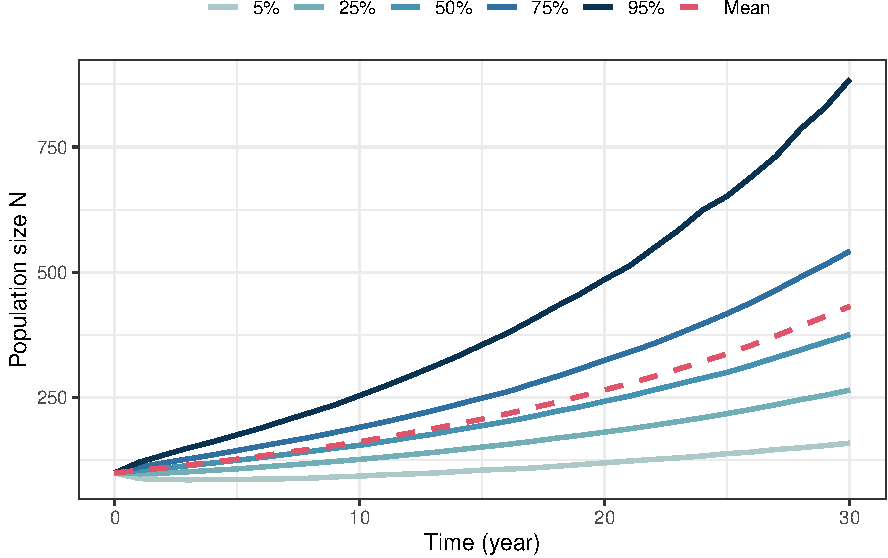
\includegraphics{DemographyCompendium_files/figure-latex/Lewontin3-1.pdf}
\caption{\label{fig:Lewontin3}Percentiles and mean from 10000 simulated trajectories of the Lewontin-Cohen model with normally distributed annual growth rates with mean \(\lambda=1.05\) and standard deviation \(\sigma=0.1\).}
\end{figure}

In contrast to the realizations, the percentiles do not fluctuate (the higher the number of realizations, the more smooth they will be). The 50\(\%\) percentile represents the median and is therefore a good representation of the `typical' population in the stochastic environment. The mean population size (shown in red on figure \ref{fig:Lewontin3}) is not a good measure of the typical population, because only only one or a few realizations reaching very high values can have a large impact on this value. Thus, for stochastic growth models the long-term growth rate of the median population is a better fitness measure than the long-term growth rate of the mean population. In extreme cases when the variance of the annual growth rates is large, the expected population size can increase exponentially because a few realizations reach extremely high values, while the median population size is declining and each realization will eventually go extinct with probability 1.
We will get back to this below.

\textless br

\hypertarget{the-stochastic-growth-rate}{%
\subsection{The stochastic growth rate}\label{the-stochastic-growth-rate}}

First, we consider the growth rate of the mean population size, although we already know this is not the best measure for the typical population. Because we assumed that the \(\Lambda_t\)'s are IID (see above), the expected population size after \(t\) time steps is given by

\begin{align}
\text{E}[N_t]&=N_0\text{E}\left[\prod_{i=0}^{t-1} \Lambda_i\right] =N_0\prod_{i=0}^{t-1}\text{E}[\Lambda_i] =N_0\lambda^t.
\label{eq:MeanGrowth}
\end{align}

Thus, the expected population size grows at the rate \(\lambda\) (the mean of the annual growth rate), just like a population growing exponentially in a constant environment. Note that \(\lambda\) does not depend on the variance of the annual growth rates.

To derive the long-term growth of the `typical' population (the socalled \textbf{stochastic growth rate}) we look at the Lewontin-Cohen process (equation \eqref{eq:Lewontin1}) on log scale:

\begin{align}
\ln N_t&=\ln \Lambda_{t-1}+\ln\Lambda_{t-2}+...+\ln\Lambda_{1}+\ln\Lambda_0+\ln N_0\\ &=\ln N_0+ \sum_{i=0}^{t-1} \ln \Lambda_i.
\label{eq:Lewontin2}
\end{align}
Here, the first term \(\ln N_0\) is a constant (since the initial population size is given). The second term is a sum over all the stochastic growth increments on log scale. Together with the IID assumption, this allows us to take advantage of the central limit theorem (if you need a reminder: \url{https://en.wikipedia.org/wiki/Central_limit_theorem}): As as the number of time steps \(t\) approaches infinity the sum will be normally distributed with mean \(t\text{E}[\ln\Lambda_t]\) and variance \(t\text{Var}(\ln\Lambda_t)\).

Thus, the expected value of \(\ln N_t\) is given by

\begin{align}
\text{E}[\ln N_t]=\ln N_0 + \text{E}\left[\sum_{i=0}^{t-1} \ln \Lambda_i\right]=\ln N_0 + t\text{E}[\ln\Lambda_t]
\end{align}
This expectation grows (or declines) linearly over time \(t\), and the slope of this line is the mean \(\text{E}[\ln\Lambda_t]=r_s\). The constant \(r_s\) is called the \textbf{stochastic growth rate} (note that the name can be misleading, as this is a constant, and not a stochastic variable).

Importantly, the stochastic growth rate is generally lower than the growth rate of the mean population, \(r=\ln \lambda=\ln(\text{E}[\Lambda_t])\), unless the variance of the annual growth rates is zero (then they are the same). The stochastic growth rate describes the growth of the median population size. The population size \(N_t\) is lognormally distributed because \(\ln N_t\) is lognormally distributed (due to the central limit theorem), and the lognormal distribution is skewed. In the lognormal distribution median is always lower than (or equal to) the mean, and is a better descriptor of the \emph{central tendency} (or as we put it, it provides a better description of a typical population growth trajectory than the mean).

How different are the two growth rates, and can we express this difference as a function of the variance of the \(\Lambda_t\), \(\sigma^2\)? Yes, \citet{Lewontin1} showed (using a Taylor expansion of \(\ln \Lambda_t\) around \(\lambda\); not within the scope of this compendium) that the stochastic growth rate \(r_S\) can be written as

\begin{align} 
r_s\approx r-\frac{\sigma^2}{2\lambda^2}.
\label{eq:Taylor}
\end{align}
This equation tells us that the difference between the growth rate \(r\) in the constant environment and \(r_s\) in the stochastic environment is increasing with the value of \(\sigma^2\). Thus, we can have situations where the population growth rate \(r\) is positive, but \(r_S\) is negative. And in that case, extinction of the population (at some point) is certain.

\hypertarget{arithmetic-and-geometric-mean}{%
\subsection{Arithmetic and geometric mean}\label{arithmetic-and-geometric-mean}}

The stochastic growth rate \(r_s=\text{E}[\ln \Lambda_t]\) and the growth rate of the mean environment \(r=\ln \text{E}[\Lambda_t])\) can also be compared by considering the arithmetic and geometric mean of a series of annual growth rates \(\Lambda_t\). The arithmetic mean is given by

\begin{align} 
\lambda=\text{E}[\Lambda_t]=\frac{1}{t}\sum_{i=1}^t\Lambda_i, 
\end{align}
and the log of this value is \(r=\ln \lambda\). The geometric mean is given by

\begin{align} 
e^{\text{E}[\ln\Lambda_t]}=\left(\prod_{i=1}^t \Lambda_i \right)^{1/t},
\end{align}
and the log of this value corresponds to \(r_S=\text{E}[\ln\Lambda_t]\). In contrast to the arithmetic mean, the geometric mean depends on the variance \(\sigma^2\). The arithmetic mean will always be greater than or equal to the geometric mean, and in this case they are only equal in the constant environment (if \(\sigma^2=0\)).

The code below returns the arithmetic and geometric mean of a sequence of annual growth rates, and plots them along with the sequence:

\begin{Shaded}
\begin{Highlighting}[]
\NormalTok{AGMeans }\OtherTok{\textless{}{-}} \ControlFlowTok{function}\NormalTok{(}\AttributeTok{Tmax=}\DecValTok{100}\NormalTok{, }\AttributeTok{mean.lambda=}\FloatTok{1.05}\NormalTok{, }\AttributeTok{sd.lambda=}\NormalTok{.}\DecValTok{3}\NormalTok{)\{}
  \CommentTok{\#Use lognormal distribution to avoid negative values}
\NormalTok{  Lambdavec}\OtherTok{\textless{}{-}}\FunctionTok{rlnorm}\NormalTok{(}\AttributeTok{n=}\NormalTok{Tmax, }\FunctionTok{log}\NormalTok{(mean.lambda)}\SpecialCharTok{{-}}\NormalTok{.}\DecValTok{5}\SpecialCharTok{*}\FunctionTok{log}\NormalTok{(}\DecValTok{1}\SpecialCharTok{+}\NormalTok{ sd.lambda}\SpecialCharTok{\^{}}\DecValTok{2}\SpecialCharTok{/}\NormalTok{(mean.lambda}\SpecialCharTok{\^{}}\DecValTok{2}\NormalTok{)), }\AttributeTok{sdlog=}\FunctionTok{sqrt}\NormalTok{(}\FunctionTok{log}\NormalTok{(}\DecValTok{1}\SpecialCharTok{+}\NormalTok{ sd.lambda}\SpecialCharTok{\^{}}\DecValTok{2}\SpecialCharTok{/}\NormalTok{(mean.lambda}\SpecialCharTok{\^{}}\DecValTok{2}\NormalTok{))))}
\NormalTok{   geomLambda}\OtherTok{\textless{}{-}} \FunctionTok{exp}\NormalTok{(}\FunctionTok{mean}\NormalTok{(}\FunctionTok{log}\NormalTok{(Lambdavec)))}
\NormalTok{   meanLambda }\OtherTok{\textless{}{-}} \FunctionTok{mean}\NormalTok{(Lambdavec)}
  \FunctionTok{data.frame}\NormalTok{(}\StringTok{"Time"}\OtherTok{=}\DecValTok{0}\SpecialCharTok{:}\NormalTok{(}\FunctionTok{length}\NormalTok{(Lambdavec)}\SpecialCharTok{{-}}\DecValTok{1}\NormalTok{), }\StringTok{"Lambda"}\OtherTok{=}\NormalTok{Lambdavec, }\StringTok{"Geometric"}\OtherTok{=}\NormalTok{geomLambda, }\StringTok{"Arithmetic"}\OtherTok{=}\NormalTok{meanLambda)}
\NormalTok{\}}

\FunctionTok{set.seed}\NormalTok{(}\DecValTok{20}\NormalTok{) }

\NormalTok{GetMeans }\OtherTok{\textless{}{-}} \FunctionTok{AGMeans}\NormalTok{()}
\NormalTok{Geometric }\OtherTok{\textless{}{-}}\NormalTok{ GetMeans}\SpecialCharTok{$}\NormalTok{Geometric[}\DecValTok{1}\NormalTok{]}
\NormalTok{Arithmetic }\OtherTok{\textless{}{-}}\NormalTok{ GetMeans}\SpecialCharTok{$}\NormalTok{Arithmetic[}\DecValTok{1}\NormalTok{]}
\FunctionTok{ggplot}\NormalTok{(GetMeans) }\SpecialCharTok{+} 
  \FunctionTok{geom\_point}\NormalTok{(}\FunctionTok{aes}\NormalTok{(}\AttributeTok{x=}\NormalTok{Time, }\AttributeTok{y=}\NormalTok{Lambda), }\AttributeTok{size=}\DecValTok{2}\NormalTok{, }\AttributeTok{col=}\DecValTok{8}\NormalTok{)}\SpecialCharTok{+}
  \FunctionTok{geom\_hline}\NormalTok{(}\AttributeTok{yintercept=}\NormalTok{ Geometric,}\AttributeTok{lwd=}\FloatTok{1.2}\NormalTok{, }\AttributeTok{linetype=}\DecValTok{2}\NormalTok{,}\AttributeTok{col=}\DecValTok{2}\NormalTok{)}\SpecialCharTok{+}
  \FunctionTok{geom\_text}\NormalTok{(}\FunctionTok{aes}\NormalTok{(}\DecValTok{10}\NormalTok{, Geometric, }\AttributeTok{label =} \StringTok{"Geometric mean"}\NormalTok{, }\AttributeTok{vjust =}  \DecValTok{2}\NormalTok{), }\AttributeTok{col=}\DecValTok{2}\NormalTok{)}\SpecialCharTok{+}
  \FunctionTok{geom\_hline}\NormalTok{(}\AttributeTok{yintercept=}\NormalTok{Arithmetic,}\AttributeTok{lwd=}\FloatTok{1.2}\NormalTok{, }\AttributeTok{col=}\DecValTok{4}\NormalTok{)}\SpecialCharTok{+}
  \FunctionTok{geom\_text}\NormalTok{(}\FunctionTok{aes}\NormalTok{(}\DecValTok{10}\NormalTok{,  Arithmetic, }\AttributeTok{label =} \StringTok{"Arithmetic mean"}\NormalTok{, }\AttributeTok{vjust =} \SpecialCharTok{{-}}\DecValTok{2}\NormalTok{),}\AttributeTok{col=}\DecValTok{4}\NormalTok{)}\SpecialCharTok{+}
  \FunctionTok{theme\_bw}\NormalTok{() }\SpecialCharTok{+}
  \FunctionTok{theme}\NormalTok{(}\AttributeTok{legend.position =} \StringTok{"none"}\NormalTok{ )}\SpecialCharTok{+}
  \FunctionTok{labs}\NormalTok{( }\AttributeTok{x=}\StringTok{"Time (year)"}\NormalTok{, }\AttributeTok{y=}\FunctionTok{expression}\NormalTok{(Lambda[t])) }\CommentTok{\#Axis labels}
\end{Highlighting}
\end{Shaded}

\begin{figure}
\centering
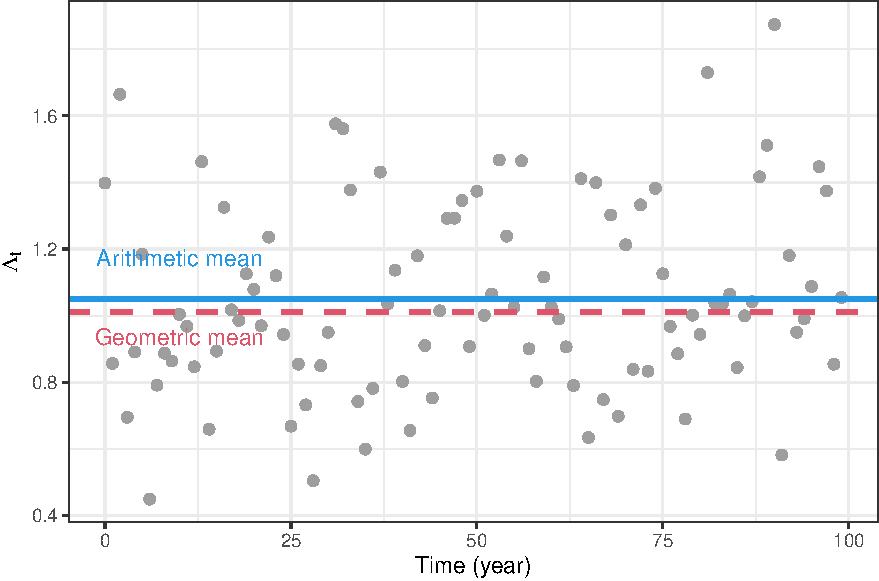
\includegraphics{DemographyCompendium_files/figure-latex/arithmetic-1.pdf}
\caption{\label{fig:arithmetic}Arithmetic and geometric mean of a sequence of annual growth rates \(\Lambda_t\), with annual mean \(\lambda=1.05\) and annual standard deviation \(\sigma=0.3\)}
\end{figure}

\hypertarget{bet-hedging}{%
\subsection{Bet-hedging}\label{bet-hedging}}

From an evolutionary perspective, the Lewontin-Cohen model is an important starting point to describe fitness in a stochastic environment (\(r_S\)), and understand how it differs from the fitness in a the mean environment (\(r\)). In particular, it provides a baseline model to describe strategies of bet-hedging. Since \(r_S\) depends on both \(r\) and \(\sigma^2\), organisms in stochastic environments can improve their fitness through increasing the mean \(r\), or reducing the variance \(\sigma^2\). \textbf{Bet-hedging} strategies \emph{reduce the variance, at the cost of also reducing the arithmetic mean fitness}. As a result the fitness in the stochastic environment \(r_S\) is optimized.

Bet-hedging can operate through two main mechanisms, or a combination:

\begin{itemize}
\item
  \textbf{Conservative bet hedging} refers to strategies that `play it safe', where the organism does not optimize its fitness for any given environment, but in the long run still come out with a higher geometric mean fitness. For instance, a bird could lay a low number of eggs at each reproduction to improve the survival of their offspring, thus reducing the variance but at the cost of a lower than optimum clutch size in the mean environment.
\item
  \textbf{Diversifying bet-hedging} are strategies that avoid risk by `not putting all eggs in one basket', for instance by producing offspring with a high diversity of phenotypes. While this will certainly increase the variance in fitness among the offspring, it reduces the variance of the parent. Again, it is not truly bet-hedging unless the parent also pays a cost in terms of lowered arithmetic mean fitness (here corresponding to producing offspring of just one type optimal for the mean environment).
\end{itemize}

\hypertarget{stochastic-growth-of-structured-populations}{%
\section{Stochastic growth of structured populations}\label{stochastic-growth-of-structured-populations}}

In structured populations, the stochastic population dynamics are more complex because the annual population growth rates are no longer `IID' (Independently and Identically Distributed). For the Lewontin-Cohen model this was a key assumption that allowed us to use the central limit theorem to derive the stochastic growth rate. But in structured populations, the annual growth rates will show \emph{autocorrelation} (a memory in the process) because the population structure itself generates lags in the growth process. Even if there is some stochastic environmental variable that is IID and gives rise to stochasticity in the population growth, the population growth rates will not be IID.

For instance, if the environment is particularly good for reproduction one year, this can lead to a `strong' year class (cohort) that persists in the population over time and affects the population growth rate for potentially many years. We get `waves' of such cohorts that generate long-term fluctuations in the stage structure on top of the year-to-year fluctuations due to stochasticity. The long-term fluctuations create autocorrelation in the population growth process. In contrast to the population growth in a constant environment, where the transient initial fluctuations disappear over time (chapter \ref{s03-MatrixModels}), the transients will never really disappear in a stochastic environment Instead, the population structure will fluctuate around the stable structure.

How can we then study population growth and fitness of structured populations in stochastic environments? We can always do simulations (projections) of the population growth process, as we did for the Lewontin-Cohen model, and we can define the stochastic growth rate based on a (long) sequence of generated populaton sizes. In addition, under the assumption of small fluctuations it is possible to approximate the stochastic growth rate as a function of the mean, variance and covariance of matrix elements, as we will see below. First we will define a general model to describe the growth of structured populations in a time-varying environment.

\hypertarget{defining-the-process-1}{%
\subsection{Defining the process}\label{defining-the-process-1}}

In a fluctuating environment, the projection matrix \(\mathbf{A}\) will take a new value each time step, so that the population growth over many time steps is given by matrix multiplication from time 0:

\[\mathbf{n}_{t+1}=\mathbf{A}_{t}\mathbf{n}_{t}=\mathbf{A}_{t}\mathbf{A}_{t-1}\mathbf{A}_{t-2}\cdots\mathbf{A}_{0}\mathbf{n}_{t}\]

When these time-dependent projection matrices \(\mathbf{A}_t\) are generated by a random process each time step, we have a \textbf{stochastic matrix model}. There are two main approaches to study the dynamics of such a model:

\begin{itemize}
\item
  The \emph{environment-blind} approach generates a set of projection matrices e.g.~from each year of a study, and then samples among these to generate a new stochastic sequence of matrices according to a given sampling model (e.g.~a Markov process). In this case, correlation between vital rates of the projection matrix are automatically incorporated since the entire matrix is sampled.
\item
  The \emph{environment-specific} approach specifies each matrix element (e.g.~fertility and survival coefficients) as a stochastic variable with a mean, variance and potentially covariance among matrix elements. Together, all the stochastic elements in the model define a multivariate vector with a given distribution (specified by a vector of means and a variance-covariance matrix). This approach is more complex, but often better suited to account for explicit relationships between the vital rates and environmental variables such as temperature.
\end{itemize}

\hypertarget{bird-example-16}{%
\subsubsection*{Bird example}\label{bird-example-16}}
\addcontentsline{toc}{subsubsection}{Bird example}

We will again use the bird example introduced in @ref\{birdtable\} and following chapters, and now consider a stochastic version of the matrix model for this bird with pre-reproductive census (chapter \ref{s03-MatrixModels}).

In the constant environment, the pre-reproductive projection matrix for the songbird was given by (\eqref{eq:Prerep}):

\begin{align}
\begin{split}
\mathbf{A}=\left[\begin{matrix} f_1 & f_2 &f_3  \\ s_1 &0&0\\ 0 & s_2 &0  \\  \end{matrix}\right]=\left[\begin{matrix} 0 &0.6 &1.2  \\ 0.9 &0&0\\ 0 & 0.6 &0  \\  \end{matrix}\right].
\end{split}
\end{align}

We will now add stochasticity to the elements of this matrix, by allowing the fertilities and survival probabilities to fluctuate randomly. Adding stochasticity needs to be done with some care: Survival probabilities are restricted to be between 0 and 1, and fertilities must always be non-negative. A good idea is to use appropriate \emph{scaling functions} (link functions) where stochasticity can be added as a normally distributed variable on the link scale. For this example, we will assume a log-link function for the fertilities, and a log log link function for the survival (but in general many other kinds of functions are also possible):

\[f_{it}=\exp(\beta_{fi}+\varepsilon_{fit})\]

\[s_{it}=\exp(-\exp(-\beta_{si}-\varepsilon_{sit}))).\]

Here \(\varepsilon_{fi}\) and \(\varepsilon_{si}\) are random (stochastic) variables assumed to follow a normal distribution with mean 0 and standard deviation \(\sigma_{fi}\) and \(\sigma_{si}\), respectively. The constants \(\beta_{fi}\) and \(\beta_{si}\) define the fertility and survival when the standard deviations (and thus the \(\varepsilon\)'s) are zero. Note that this is just one of several ways to model stochasticity in survival and fertility.

\hypertarget{plot-one-realization-of-the-process-1}{%
\subsection*{Plot one realization of the process}\label{plot-one-realization-of-the-process-1}}
\addcontentsline{toc}{subsection}{Plot one realization of the process}

To add stochasticity to the fertilities and survival probabilities in the projection matrix, we will use the function \texttt{mvrnorm()} from the package \texttt{MASS}, which generates values from the multivariate normal distribution. The function \texttt{mvrnorm} uses a variance-covariance matrix as one of its input variables, and here we will for simplicity assume no covariance. We also assume that stochasticity only affects survival and fertility coefficients, and that these follow log-log link and log-link functions, respectively.

The following function generates a series of random projection matrices using the \texttt{mvrnorm()} function from the package \texttt{MASS} to add stochasticity in survival and fecundity. The matrices are returned as an array, which is an extension of the ´matrix´ object to multiple dimensions. Here we have three dimensions: Time (\texttt{Tmax}), \(k\) and \(k\), where \(k\) is the number of rows and columns of the projection matrix.

Inputs to the function are the projection matrix in the constant environment \(\mathbf{A}\), its main components \(\mathbf{U}\) and \(\mathbf{F}\) (used to separate out survival coefficients and fertilities), and two vectors defining the variance in scaled fertility and survival. Each vector needs to be of length \(k\) corresponding to the number of stages in the population.

\begin{Shaded}
\begin{Highlighting}[]
\NormalTok{Amat.array }\OtherTok{\textless{}{-}} \ControlFlowTok{function}\NormalTok{(MatA, MatU, MatF, }\AttributeTok{tmax=}\DecValTok{30}\NormalTok{, }\AttributeTok{VarF=}\FunctionTok{rep}\NormalTok{(}\FloatTok{0.03}\NormalTok{, }\DecValTok{3}\NormalTok{), }\AttributeTok{VarS=}\FunctionTok{rep}\NormalTok{(}\FloatTok{0.03}\NormalTok{, }\DecValTok{3}\NormalTok{))\{}
\NormalTok{  SplitU }\OtherTok{\textless{}{-}} \FunctionTok{DecomposeU}\NormalTok{(MatU) }\CommentTok{\#Split survival/transition matrix}
\NormalTok{  SplitF }\OtherTok{\textless{}{-}} \FunctionTok{DecomposeF}\NormalTok{(MatF) }\CommentTok{\#Split fertility matrix}
\NormalTok{  Gmat }\OtherTok{\textless{}{-}}\NormalTok{ SplitU}\SpecialCharTok{$}\NormalTok{Gmat }\CommentTok{\#Transition matrix}
\NormalTok{  Svec }\OtherTok{\textless{}{-}}\NormalTok{ SplitU}\SpecialCharTok{$}\NormalTok{Survival }\CommentTok{\#Survival vector}
\NormalTok{  Beta.S }\OtherTok{\textless{}{-}} \SpecialCharTok{{-}}\FunctionTok{log}\NormalTok{(}\SpecialCharTok{{-}}\FunctionTok{log}\NormalTok{(Svec)) }\CommentTok{\#Define beta for constant environment (no variance)}
\NormalTok{  Qmat }\OtherTok{\textless{}{-}}\NormalTok{ SplitF}\SpecialCharTok{$}\NormalTok{Qmat }\CommentTok{\#Offspring transition matrix}
\NormalTok{  Fvec }\OtherTok{\textless{}{-}}\NormalTok{ SplitF}\SpecialCharTok{$}\NormalTok{Fertility }\CommentTok{\#Fertility vector}
\NormalTok{  Beta.F }\OtherTok{\textless{}{-}} \FunctionTok{log}\NormalTok{(Fvec) }\CommentTok{\#Define beta for constant environment (no variance)}
\NormalTok{  k }\OtherTok{\textless{}{-}} \FunctionTok{length}\NormalTok{(Svec) }\CommentTok{\#Number of matrix classes (used in for{-}loop)}
\NormalTok{  SigMat }\OtherTok{\textless{}{-}} \FunctionTok{diag}\NormalTok{(}\FunctionTok{c}\NormalTok{(VarS, VarF))}\CommentTok{\# variance covariance matrix }
\NormalTok{  SFTime }\OtherTok{\textless{}{-}} \FunctionTok{mvrnorm}\NormalTok{(tmax, }\AttributeTok{mu=}\FunctionTok{c}\NormalTok{(Beta.S, Beta.F), }\AttributeTok{Sigma=}\NormalTok{SigMat)}\CommentTok{\#Draw scaled values from multivariate normal distribution.}
\NormalTok{  SvecTime}\OtherTok{\textless{}{-}}   \FunctionTok{exp}\NormalTok{(}\SpecialCharTok{{-}}\FunctionTok{exp}\NormalTok{(}\SpecialCharTok{{-}}\NormalTok{SFTime[,}\DecValTok{1}\SpecialCharTok{:}\NormalTok{k])) }\CommentTok{\#Rescaled survival probabilities (loglog link)}
\NormalTok{  FvecTime}\OtherTok{\textless{}{-}} \FunctionTok{exp}\NormalTok{(SFTime[,(k}\SpecialCharTok{+}\DecValTok{1}\NormalTok{)}\SpecialCharTok{:}\NormalTok{(}\DecValTok{2}\SpecialCharTok{*}\NormalTok{k)]) }\CommentTok{\#Rescaled fertilities  (log link)}
\CommentTok{\#Use values to build one projection matrix for each time step, store them in  array}
\NormalTok{  A.array }\OtherTok{\textless{}{-}} \FunctionTok{array}\NormalTok{(}\ConstantTok{NA}\NormalTok{,}\AttributeTok{dim=}\FunctionTok{c}\NormalTok{(k,k,tmax))}
  \ControlFlowTok{for}\NormalTok{ (i }\ControlFlowTok{in} \DecValTok{1}\SpecialCharTok{:}\NormalTok{tmax)\{}
\NormalTok{    Smat }\OtherTok{\textless{}{-}} \FunctionTok{diag}\NormalTok{(SvecTime[i,])}
\NormalTok{    Fmat }\OtherTok{\textless{}{-}} \FunctionTok{diag}\NormalTok{(FvecTime[i,])}
\NormalTok{    A.array[,,i] }\OtherTok{\textless{}{-}}\NormalTok{   Gmat}\SpecialCharTok{\%*\%}\NormalTok{Smat}\SpecialCharTok{+}\NormalTok{Qmat}\SpecialCharTok{\%*\%}\NormalTok{Fmat}
\NormalTok{  \}}
\FunctionTok{return}\NormalTok{(}\StringTok{"Amats"} \OtherTok{=}\NormalTok{ A.array)}
\NormalTok{\}}
\end{Highlighting}
\end{Shaded}

Using this function to generate a sequence of stochastic projection matrices, we can make another function to project the population growth over time. This projection is similar to the one we used for the constant environment (chapter \ref{s03-MatrixModels}), except that for each time step we now use a new different matrix due to stochasticity. The function below returns a data frame with the size of each stage over time, including the initial sizes provided in \texttt{n0}.

\begin{Shaded}
\begin{Highlighting}[]
\NormalTok{projection.stochastic }\OtherTok{\textless{}{-}}\ControlFlowTok{function}\NormalTok{(Amats, n0)\{}
\NormalTok{    Tmax }\OtherTok{\textless{}{-}} \FunctionTok{dim}\NormalTok{(Amats)[}\DecValTok{3}\NormalTok{]}
\NormalTok{    k }\OtherTok{\textless{}{-}} \FunctionTok{dim}\NormalTok{(Amats)[}\DecValTok{1}\NormalTok{]}
    \ControlFlowTok{if}\NormalTok{(}\FunctionTok{length}\NormalTok{(n0)}\SpecialCharTok{!=}\NormalTok{k)\{}
      \FunctionTok{warning}\NormalTok{(}\StringTok{"n0 should have length k corresponding to number of stages in the Amats object"}\NormalTok{)}
\NormalTok{      \}}
\NormalTok{    Nmat }\OtherTok{\textless{}{-}} \FunctionTok{matrix}\NormalTok{(}\ConstantTok{NA}\NormalTok{,}\AttributeTok{nrow=}\NormalTok{ Tmax}\SpecialCharTok{+}\DecValTok{1}\NormalTok{, }\AttributeTok{ncol=}\NormalTok{k)}
\NormalTok{    Nmat[}\DecValTok{1}\NormalTok{,] }\OtherTok{\textless{}{-}}\NormalTok{ n0}
\NormalTok{  cnames }\OtherTok{\textless{}{-}} \FunctionTok{paste}\NormalTok{(}\StringTok{"n"}\NormalTok{, }\DecValTok{1}\SpecialCharTok{:}\NormalTok{k, }\AttributeTok{sep=}\StringTok{""}\NormalTok{)}
\NormalTok{  timesteps }\OtherTok{\textless{}{-}} \DecValTok{0}\SpecialCharTok{:}\NormalTok{Tmax}
    \ControlFlowTok{for}\NormalTok{(i }\ControlFlowTok{in} \DecValTok{2}\SpecialCharTok{:}\NormalTok{(Tmax}\SpecialCharTok{+}\DecValTok{1}\NormalTok{))\{  }
\NormalTok{        Nmat[i,] }\OtherTok{\textless{}{-}}\NormalTok{ Amats[,,i}\DecValTok{{-}1}\NormalTok{] }\SpecialCharTok{\%*\%}\NormalTok{ Nmat[i}\DecValTok{{-}1}\NormalTok{,]}
\NormalTok{        \}}
\NormalTok{  frame }\OtherTok{\textless{}{-}} \FunctionTok{data.frame}\NormalTok{(timesteps,Nmat)}
  \FunctionTok{colnames}\NormalTok{(frame) }\OtherTok{\textless{}{-}} \FunctionTok{c}\NormalTok{(}\StringTok{"time"}\NormalTok{, cnames)}
\NormalTok{  frame}
\NormalTok{\}}
\end{Highlighting}
\end{Shaded}

\hypertarget{bird-example-17}{%
\subsubsection*{Bird example}\label{bird-example-17}}
\addcontentsline{toc}{subsubsection}{Bird example}

\begin{Shaded}
\begin{Highlighting}[]
\FunctionTok{set.seed}\NormalTok{(}\DecValTok{20}\NormalTok{)}

\CommentTok{\#Generate sequence of stochastic matrices:}
\NormalTok{Amats.bird }\OtherTok{\textless{}{-}} \FunctionTok{Amat.array}\NormalTok{(}\AttributeTok{MatA=}\NormalTok{Abird.pre, }\AttributeTok{MatU=}\NormalTok{Ubird.pre, }\AttributeTok{MatF=}\NormalTok{Fbird.pre, }\AttributeTok{tmax=}\DecValTok{20}\NormalTok{, }\AttributeTok{VarF=}\FunctionTok{rep}\NormalTok{(}\FloatTok{0.03}\NormalTok{, }\DecValTok{3}\NormalTok{), }\AttributeTok{VarS=}\FunctionTok{rep}\NormalTok{(}\FloatTok{0.03}\NormalTok{, }\DecValTok{3}\NormalTok{)) }

\CommentTok{\#Project growth:}
\NormalTok{stochastic.bird }\OtherTok{\textless{}{-}} \FunctionTok{projection.stochastic}\NormalTok{(}\AttributeTok{Amats =}\NormalTok{ Amats.bird, }\AttributeTok{n0=}\FunctionTok{c}\NormalTok{(}\DecValTok{10}\NormalTok{,}\DecValTok{10}\NormalTok{,}\DecValTok{10}\NormalTok{))}

\CommentTok{\#Long format for plotting:}
\NormalTok{stochastic.bird.long }\OtherTok{\textless{}{-}}\NormalTok{ stochastic.bird }\SpecialCharTok{\%\textgreater{}\%} \FunctionTok{pivot\_longer}\NormalTok{(}\FunctionTok{c}\NormalTok{(}\SpecialCharTok{{-}}\NormalTok{time),}
               \AttributeTok{names\_to =} \StringTok{"AgeClass"}\NormalTok{, }\AttributeTok{values\_to =} \StringTok{"Value"}\NormalTok{)}

\CommentTok{\#Plot:}
\FunctionTok{ggplot}\NormalTok{(stochastic.bird.long) }\SpecialCharTok{+} 
  \FunctionTok{geom\_line}\NormalTok{(}\FunctionTok{aes}\NormalTok{(}\AttributeTok{x=}\NormalTok{time, }\AttributeTok{y=}\NormalTok{Value, }\AttributeTok{col=}\NormalTok{AgeClass, }\AttributeTok{linetype=}\NormalTok{AgeClass), }\AttributeTok{lwd=}\FloatTok{1.2}\NormalTok{)}\SpecialCharTok{+}
  \FunctionTok{geom\_point}\NormalTok{(}\FunctionTok{aes}\NormalTok{(}\AttributeTok{x=}\NormalTok{time, }\AttributeTok{y=}\NormalTok{Value, }\AttributeTok{col=}\NormalTok{AgeClass), }\AttributeTok{size=}\DecValTok{3}\NormalTok{)}\SpecialCharTok{+}
  \FunctionTok{theme\_bw}\NormalTok{() }\SpecialCharTok{+}
  \FunctionTok{scale\_color\_manual}\NormalTok{(}\AttributeTok{values=}\NormalTok{colors3)}\SpecialCharTok{+} 
  \FunctionTok{scale\_linetype\_manual}\NormalTok{(}\AttributeTok{values=}\FunctionTok{c}\NormalTok{(}\DecValTok{1}\NormalTok{,}\DecValTok{2}\NormalTok{,}\DecValTok{3}\NormalTok{))}\SpecialCharTok{+}  
  \FunctionTok{labs}\NormalTok{( }\AttributeTok{x=}\StringTok{"Time (year)"}\NormalTok{, }\AttributeTok{y=}\StringTok{"Age class size"}\NormalTok{)  }
\end{Highlighting}
\end{Shaded}

\begin{figure}
\centering
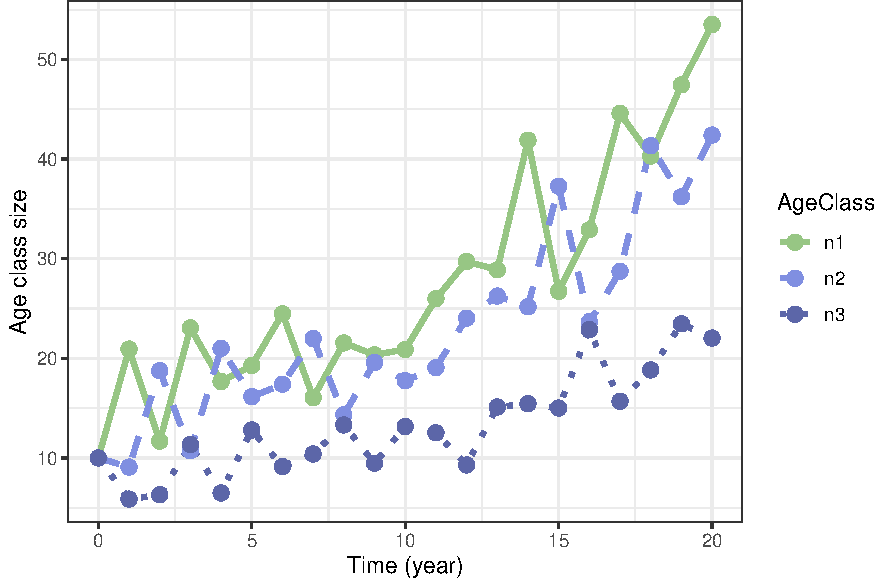
\includegraphics{DemographyCompendium_files/figure-latex/birdstochastic1-1.pdf}
\caption{\label{fig:birdstochastic1}One realization of stochastic growth in the bird example with pre-reproductive census, with stochastic survival and fertility coefficients.}
\end{figure}

Figure \ref(fig:birdstochastic1) shows the growth of each stage of the bird population over 20 years, starting from a population with 10 birds in each age class.The highest number of fluctuations is found for the first age class, and we can see that the peaks in this age class are followed by peaks in year class 2 and 3 in the following years, as the cohort grows through the population.

We can also plot the total population size, by summing up the values of the age classes for each year, as shown in figure \ref{fig:birdstochastic2}:

\begin{Shaded}
\begin{Highlighting}[]
\CommentTok{\#Sum up population sizes}
\NormalTok{stochastic.bird}\SpecialCharTok{$}\NormalTok{Ntot }\OtherTok{\textless{}{-}} \FunctionTok{apply}\NormalTok{(stochastic.bird[,}\SpecialCharTok{{-}}\DecValTok{1}\NormalTok{],}\DecValTok{1}\NormalTok{,sum)}


\FunctionTok{ggplot}\NormalTok{(stochastic.bird) }\SpecialCharTok{+} 
  \FunctionTok{geom\_line}\NormalTok{(}\FunctionTok{aes}\NormalTok{(}\AttributeTok{x=}\NormalTok{time, }\AttributeTok{y=}\NormalTok{Ntot), }\AttributeTok{lwd=}\FloatTok{1.2}\NormalTok{)}\SpecialCharTok{+}
  \FunctionTok{geom\_point}\NormalTok{(}\FunctionTok{aes}\NormalTok{(}\AttributeTok{x=}\NormalTok{time, }\AttributeTok{y=}\NormalTok{Ntot), }\AttributeTok{size=}\DecValTok{3}\NormalTok{)}\SpecialCharTok{+}
  \FunctionTok{theme\_bw}\NormalTok{() }\SpecialCharTok{+}
  \FunctionTok{labs}\NormalTok{( }\AttributeTok{x=}\StringTok{"Time (year)"}\NormalTok{, }\AttributeTok{y=}\StringTok{"Populatipn size N"}\NormalTok{)  }
\end{Highlighting}
\end{Shaded}

\begin{figure}
\centering
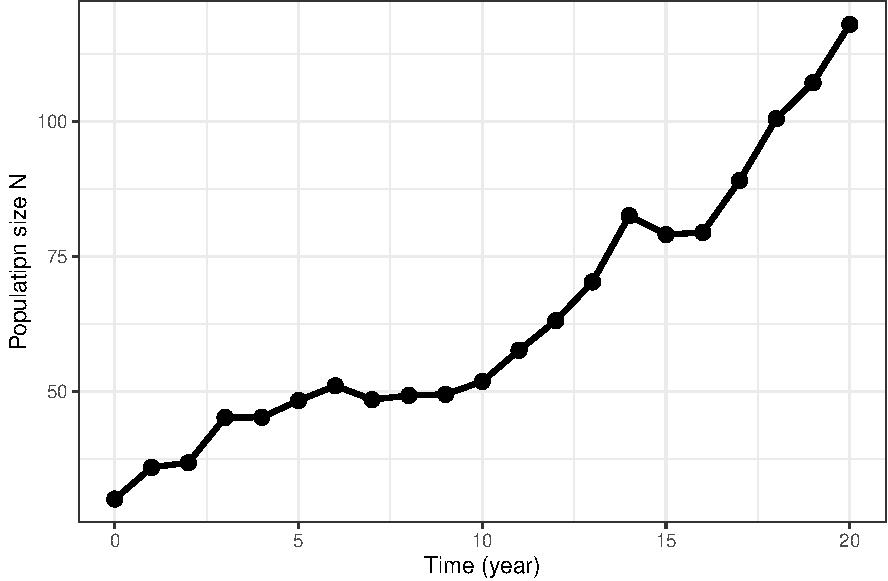
\includegraphics{DemographyCompendium_files/figure-latex/birdstochastic2-1.pdf}
\caption{\label{fig:birdstochastic2}Same process as in figure \ref{fig:birdstochastic1}, with age classes summed up to get the total population size.}
\end{figure}

\hypertarget{plot-many-realizations-of-the-process-1}{%
\subsection*{Plot many realizations of the process}\label{plot-many-realizations-of-the-process-1}}
\addcontentsline{toc}{subsection}{Plot many realizations of the process}

Instead of looking at just one realization of the stochastic growth process, it is often useful to generate multiple realizations and look at summary statistics and properties for these, as we have seen already for the Lewontin-Cohen-process.

The following function generates a series of matrices \texttt{nsim} times, each series of length \texttt{Tmax}, and returns the projected total population size over time for each series, in a data frame. Other input variables are the constant matrices and variance vectors, and initial population vector.

\begin{Shaded}
\begin{Highlighting}[]
\NormalTok{nsim.stochastic }\OtherTok{\textless{}{-}} \ControlFlowTok{function}\NormalTok{(}\AttributeTok{nsim=}\DecValTok{100}\NormalTok{, }\AttributeTok{tmax=}\DecValTok{30}\NormalTok{, }\AttributeTok{n0=}\FunctionTok{rep}\NormalTok{(}\DecValTok{10}\NormalTok{,}\DecValTok{3}\NormalTok{), MatA, MatU, MatF, VarF, VarS)\{}
\NormalTok{  frame }\OtherTok{\textless{}{-}}  \FunctionTok{data.frame}\NormalTok{(}\StringTok{"Time"}\OtherTok{=}\DecValTok{0}\SpecialCharTok{:}\NormalTok{tmax)}
  \ControlFlowTok{for}\NormalTok{(m }\ControlFlowTok{in} \DecValTok{1}\SpecialCharTok{:}\NormalTok{nsim)\{}
\NormalTok{  AMATS }\OtherTok{\textless{}{-}} \FunctionTok{Amat.array}\NormalTok{(}\AttributeTok{MatA=}\NormalTok{MatA, }\AttributeTok{MatU=}\NormalTok{MatU, }\AttributeTok{MatF=}\NormalTok{MatF, }\AttributeTok{VarF=}\NormalTok{VarF, }\AttributeTok{VarS=}\NormalTok{VarS, }\AttributeTok{tmax=}\NormalTok{tmax)}
\NormalTok{   projectN }\OtherTok{\textless{}{-}} \FunctionTok{apply}\NormalTok{(}\FunctionTok{projection.stochastic}\NormalTok{(}\AttributeTok{Amats=}\NormalTok{AMATS, }\AttributeTok{n0=}\NormalTok{n0)[,}\SpecialCharTok{{-}}\DecValTok{1}\NormalTok{],}\DecValTok{1}\NormalTok{,sum)}
\NormalTok{  frame }\OtherTok{\textless{}{-}} \FunctionTok{cbind}\NormalTok{(frame, projectN)}
  \FunctionTok{names}\NormalTok{(frame)[m}\SpecialCharTok{+}\DecValTok{1}\NormalTok{] }\OtherTok{\textless{}{-}} \FunctionTok{paste}\NormalTok{(}\StringTok{"Rep"}\NormalTok{,m,}\AttributeTok{sep=}\StringTok{""}\NormalTok{)}
\NormalTok{  \}}
\NormalTok{  frame}
\NormalTok{\}}
\end{Highlighting}
\end{Shaded}

\hypertarget{bird-example-18}{%
\subsubsection*{Bird example}\label{bird-example-18}}
\addcontentsline{toc}{subsubsection}{Bird example}

We can now plot multiple realizations also in the bird example, as shown in figure \ref{fig:birdstochastic3}

\begin{Shaded}
\begin{Highlighting}[]
\FunctionTok{set.seed}\NormalTok{(}\DecValTok{20}\NormalTok{)}

\NormalTok{nsim.bird }\OtherTok{\textless{}{-}} \FunctionTok{nsim.stochastic}\NormalTok{(}\AttributeTok{MatA=}\NormalTok{Abird.pre, }\AttributeTok{MatU=}\NormalTok{Ubird.pre, }\AttributeTok{MatF=}\NormalTok{Fbird.pre,  }\AttributeTok{VarF=}\FunctionTok{rep}\NormalTok{(}\FloatTok{0.03}\NormalTok{, }\DecValTok{3}\NormalTok{), }\AttributeTok{VarS=}\FunctionTok{rep}\NormalTok{(}\FloatTok{0.03}\NormalTok{, }\DecValTok{3}\NormalTok{), }\AttributeTok{tmax=}\DecValTok{20}\NormalTok{, }\AttributeTok{nsim=}\DecValTok{100}\NormalTok{, }\AttributeTok{n0=}\FunctionTok{rep}\NormalTok{(}\DecValTok{10}\NormalTok{,}\DecValTok{3}\NormalTok{))}


\NormalTok{nsim.bird.long }\OtherTok{\textless{}{-}}\NormalTok{ nsim.bird }\SpecialCharTok{\%\textgreater{}\%} \FunctionTok{pivot\_longer}\NormalTok{(}\FunctionTok{c}\NormalTok{(}\SpecialCharTok{{-}}\NormalTok{Time),}
               \AttributeTok{names\_to =} \StringTok{"Rep"}\NormalTok{, }\AttributeTok{values\_to =} \StringTok{"N"}\NormalTok{)}

\FunctionTok{ggplot}\NormalTok{(nsim.bird.long) }\SpecialCharTok{+} 
  \FunctionTok{geom\_line}\NormalTok{(}\FunctionTok{aes}\NormalTok{(}\AttributeTok{x=}\NormalTok{Time, }\AttributeTok{y=}\NormalTok{N, }\AttributeTok{col=}\NormalTok{Rep), }\AttributeTok{lwd=}\NormalTok{.}\DecValTok{5}\NormalTok{)}\SpecialCharTok{+}
  \FunctionTok{scale\_color\_manual}\NormalTok{(}\AttributeTok{values=}\FunctionTok{rep}\NormalTok{(}\DecValTok{1}\NormalTok{,}\DecValTok{100}\NormalTok{))}\SpecialCharTok{+}
  \FunctionTok{theme\_bw}\NormalTok{() }\SpecialCharTok{+}
   \FunctionTok{theme}\NormalTok{(}\AttributeTok{legend.position =} \StringTok{"none"}\NormalTok{ )}\SpecialCharTok{+}
  \FunctionTok{labs}\NormalTok{( }\AttributeTok{x=}\StringTok{"Time (year)"}\NormalTok{, }\AttributeTok{y=}\StringTok{"Population size N"}\NormalTok{) }
\end{Highlighting}
\end{Shaded}

\begin{figure}
\centering
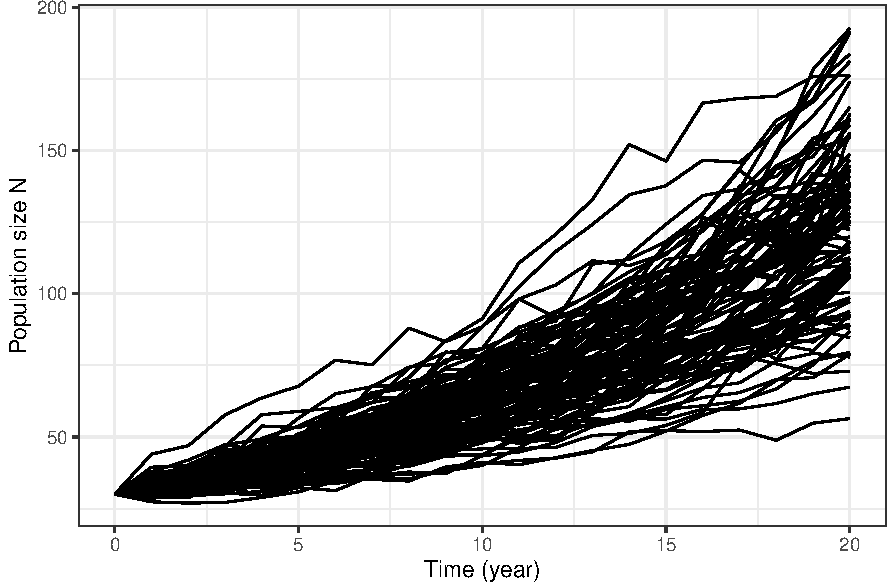
\includegraphics{DemographyCompendium_files/figure-latex/birdstochastic3-1.pdf}
\caption{\label{fig:birdstochastic3}100 realizations of the stochastic bird growth process with same parameters as in figure \ref{fig:birdstochastic2}.}
\end{figure}

To estimate the stochastic growth rate \(r_S\) from multiple realisations, we can use the following function (this measure is based on the mean of the annual growth increments of \(\ln N\)):

\begin{Shaded}
\begin{Highlighting}[]
\NormalTok{diffmat }\OtherTok{\textless{}{-}} \FunctionTok{apply}\NormalTok{(}\FunctionTok{log}\NormalTok{(nsim.bird[,}\SpecialCharTok{{-}}\DecValTok{1}\NormalTok{]),}\DecValTok{2}\NormalTok{,diff)}
\NormalTok{rS }\OtherTok{\textless{}{-}} \FunctionTok{mean}\NormalTok{(}\FunctionTok{apply}\NormalTok{(diffmat,}\DecValTok{2}\NormalTok{,mean))}
\end{Highlighting}
\end{Shaded}

In this example, the stochastic growth rate is \(r_S\approx\) 0.07.

\hypertarget{plot-percentiles-from-many-realizations-1}{%
\subsection*{Plot percentiles from many realizations}\label{plot-percentiles-from-many-realizations-1}}
\addcontentsline{toc}{subsection}{Plot percentiles from many realizations}

As shown for the Lewontin-Cohen model we can also plot percentiles of the stochastic population trajectories from a structured model, after running multiple realizations.

\hypertarget{bird-example-19}{%
\subsubsection*{Bird example}\label{bird-example-19}}
\addcontentsline{toc}{subsubsection}{Bird example}

For the bird example with 20 time steps, we get

\begin{Shaded}
\begin{Highlighting}[]
\FunctionTok{set.seed}\NormalTok{(}\DecValTok{20}\NormalTok{)}

\CommentTok{\#Apply function to get 10 0000 realizations (can take some time)}
\NormalTok{simbird\_Large }\OtherTok{\textless{}{-}} \FunctionTok{nsim.stochastic}\NormalTok{(}\AttributeTok{MatA=}\NormalTok{Abird.pre, }\AttributeTok{MatU=}\NormalTok{Ubird.pre, }\AttributeTok{MatF=}\NormalTok{Fbird.pre,  }\AttributeTok{VarF=}\FunctionTok{rep}\NormalTok{(}\FloatTok{0.03}\NormalTok{, }\DecValTok{3}\NormalTok{), }\AttributeTok{VarS=}\FunctionTok{rep}\NormalTok{(}\FloatTok{0.03}\NormalTok{, }\DecValTok{3}\NormalTok{), }\AttributeTok{tmax=}\DecValTok{20}\NormalTok{, }\AttributeTok{nsim=}\DecValTok{10000}\NormalTok{, }\AttributeTok{n0=}\FunctionTok{rep}\NormalTok{(}\DecValTok{10}\NormalTok{,}\DecValTok{3}\NormalTok{))}

\CommentTok{\#Get the 5, 25, 50, 75, and 95 percentiles:}
\NormalTok{Percentiles2  }\OtherTok{\textless{}{-}} \FunctionTok{t}\NormalTok{(}\FunctionTok{apply}\NormalTok{(}\FunctionTok{t}\NormalTok{(simbird\_Large[,}\SpecialCharTok{{-}}\DecValTok{1}\NormalTok{]),}\DecValTok{2}\NormalTok{, quantile, }\AttributeTok{probs=}\FunctionTok{c}\NormalTok{(.}\DecValTok{05}\NormalTok{, .}\DecValTok{25}\NormalTok{, .}\DecValTok{5}\NormalTok{, .}\DecValTok{75}\NormalTok{,.}\DecValTok{95}\NormalTok{)))}

 
\CommentTok{\#Store percentiles in data frame  }
\NormalTok{BirdPercentiles }\OtherTok{\textless{}{-}} \FunctionTok{as.data.frame}\NormalTok{(}\FunctionTok{cbind}\NormalTok{(}\StringTok{"Time"}\OtherTok{=}\DecValTok{0}\SpecialCharTok{:}\NormalTok{(}\FunctionTok{dim}\NormalTok{(Percentiles2)[}\DecValTok{1}\NormalTok{]}\SpecialCharTok{{-}}\DecValTok{1}\NormalTok{),  Percentiles2))}

\NormalTok{BirdPercentiles}\SpecialCharTok{$}\NormalTok{Mean }\OtherTok{\textless{}{-}} \FunctionTok{apply}\NormalTok{(}\FunctionTok{t}\NormalTok{(simbird\_Large[,}\SpecialCharTok{{-}}\DecValTok{1}\NormalTok{]),}\DecValTok{2}\NormalTok{, mean)}

\CommentTok{\#Make long format for plotting}
\NormalTok{BirdPercentiles.long }\OtherTok{\textless{}{-}}\NormalTok{ BirdPercentiles }\SpecialCharTok{\%\textgreater{}\%} \FunctionTok{pivot\_longer}\NormalTok{(}\FunctionTok{c}\NormalTok{(}\SpecialCharTok{{-}}\NormalTok{Time),}
               \AttributeTok{names\_to =} \StringTok{"Percentile"}\NormalTok{, }\AttributeTok{values\_to =} \StringTok{"N"}\NormalTok{)}

\CommentTok{\#Make sure the order of the percentiles is correct}
\NormalTok{BirdPercentiles.long}\SpecialCharTok{$}\NormalTok{Percentile }\OtherTok{\textless{}{-}} \FunctionTok{factor}\NormalTok{(BirdPercentiles.long}\SpecialCharTok{$}\NormalTok{Percentile, }\AttributeTok{levels=}\FunctionTok{c}\NormalTok{(}\StringTok{"5\%"}\NormalTok{, }\StringTok{"25\%"}\NormalTok{, }\StringTok{"50\%"}\NormalTok{, }\StringTok{"75\%"}\NormalTok{, }\StringTok{"95\%"}\NormalTok{,}\StringTok{"Mean"}\NormalTok{))}

\FunctionTok{ggplot}\NormalTok{(BirdPercentiles.long) }\SpecialCharTok{+} 
  \FunctionTok{geom\_line}\NormalTok{(}\FunctionTok{aes}\NormalTok{(}\AttributeTok{x=}\NormalTok{Time, }\AttributeTok{y=}\NormalTok{N, }\AttributeTok{col=}\NormalTok{Percentile,}\AttributeTok{linetype=}\NormalTok{Percentile), }\AttributeTok{lwd=}\DecValTok{1}\NormalTok{)}\SpecialCharTok{+}
  \FunctionTok{scale\_color\_manual}\NormalTok{(}\AttributeTok{values=}\FunctionTok{c}\NormalTok{(colors5,}\DecValTok{2}\NormalTok{))}\SpecialCharTok{+}
   \FunctionTok{scale\_linetype\_manual}\NormalTok{(}\AttributeTok{values=}\FunctionTok{c}\NormalTok{(}\FunctionTok{rep}\NormalTok{(}\DecValTok{1}\NormalTok{,}\DecValTok{5}\NormalTok{),}\DecValTok{2}\NormalTok{))}\SpecialCharTok{+}
  \FunctionTok{theme\_bw}\NormalTok{() }\SpecialCharTok{+}
   \FunctionTok{theme}\NormalTok{(}\AttributeTok{legend.position =} \StringTok{"top"}\NormalTok{,}\AttributeTok{legend.title =} \FunctionTok{element\_blank}\NormalTok{() )}\SpecialCharTok{+}
  \FunctionTok{labs}\NormalTok{( }\AttributeTok{x=}\StringTok{"Time (year)"}\NormalTok{, }\AttributeTok{y=}\StringTok{"Population size N"}\NormalTok{) }\SpecialCharTok{+}
   \FunctionTok{guides}\NormalTok{(}\AttributeTok{color =} \FunctionTok{guide\_legend}\NormalTok{(}\AttributeTok{nrow =} \DecValTok{1}\NormalTok{, }\AttributeTok{byrow =} \ConstantTok{TRUE}\NormalTok{))}
\end{Highlighting}
\end{Shaded}

\begin{figure}
\centering
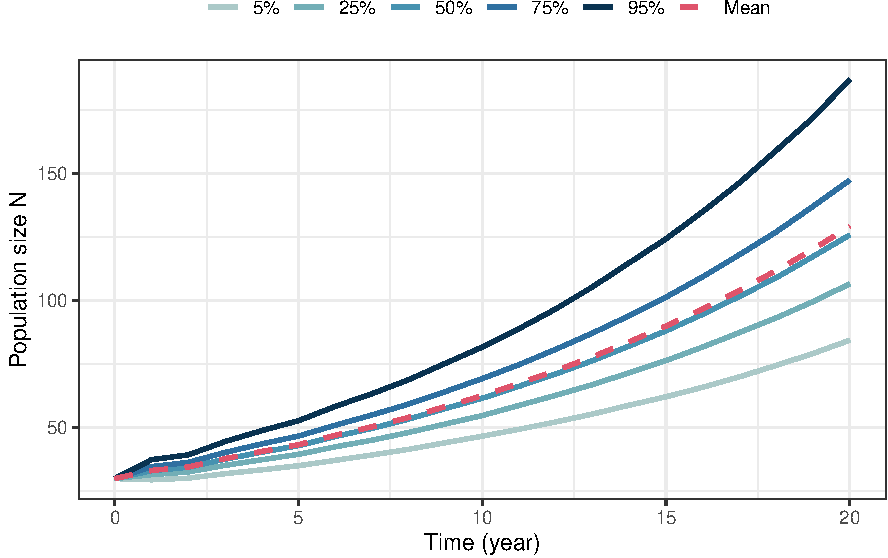
\includegraphics{DemographyCompendium_files/figure-latex/Birdstochastic4-1.pdf}
\caption{\label{fig:Birdstochastic4}Percentiles and mean from 10000 simulated trajectories of the stochastic bird model, with same parameter values as in figure \ref{fig:birdstochastic2}.}
\end{figure}

\hypertarget{stochastic-growth-rate}{%
\subsection{Stochastic growth rate}\label{stochastic-growth-rate}}

When a stochastic sequence of projection matrices is available, it can be used to project the population size over time, and the stochastic growth rate can be defined from the resulting population process as the asymptotic time-averaged growth rate:

\begin{align}
r_S=\lim_{t\to\infty}\frac{1}{t}[\ln N_t-\ln N_0],
\label{eq:StochasticRate}
\end{align}
This value can easily estimated from simulations, once the sequence of stochastic matrices is determined.

The following code can be used to calculate the stochastic growth rate following the definition of equation \eqref{eq:StochasticRate}, given a sequence of projection matrices:

\begin{Shaded}
\begin{Highlighting}[]
\CommentTok{\#the cutoff parameter removes the first time steps, where transient fluctuations can be large unless the population starts at the stable distribution. }

\NormalTok{EstimateSGR }\OtherTok{\textless{}{-}} \ControlFlowTok{function}\NormalTok{(Amats, n0, }\AttributeTok{cutoff=}\DecValTok{20}\NormalTok{)\{}
\NormalTok{  Tmax }\OtherTok{\textless{}{-}} \FunctionTok{dim}\NormalTok{(Amats)[}\DecValTok{3}\NormalTok{]}
    \ControlFlowTok{if}\NormalTok{(cutoff}\SpecialCharTok{\textgreater{}=}\NormalTok{Tmax)\{}
      \FunctionTok{warning}\NormalTok{(}\StringTok{"cutoff must be lower than the number of matrices in Amats"}\NormalTok{)}
\NormalTok{      \}}
\NormalTok{  project }\OtherTok{\textless{}{-}} \FunctionTok{projection.stochastic}\NormalTok{(}\AttributeTok{Amats=}\NormalTok{Amats, }\AttributeTok{n0=}\NormalTok{n0) }
\NormalTok{  Ntot }\OtherTok{\textless{}{-}} \FunctionTok{apply}\NormalTok{(project[,}\SpecialCharTok{{-}}\DecValTok{1}\NormalTok{],}\DecValTok{1}\NormalTok{,sum)}
\NormalTok{  logN }\OtherTok{\textless{}{-}} \FunctionTok{log}\NormalTok{(Ntot[cutoff}\SpecialCharTok{:}\FunctionTok{length}\NormalTok{(Ntot)])}
\NormalTok{  TM }\OtherTok{\textless{}{-}} \FunctionTok{length}\NormalTok{(logN)}
\NormalTok{  (logN[TM]}\SpecialCharTok{{-}}\NormalTok{logN[}\DecValTok{1}\NormalTok{])}\SpecialCharTok{/}\NormalTok{TM}
\NormalTok{\}}
\end{Highlighting}
\end{Shaded}

Note that the estimate becomes more accurate the longer the sequence, and the closer the initial population vector is to the stable distribution from the constant (mean) environment (or the higher the cutoff). If the growth rate is very large or small, numerical issues can arise affecting the estimation.

This estimate is based on only one run of the process, and the accuracy can be improved by running it many times.

\hypertarget{bird-example-20}{%
\subsubsection*{Bird example}\label{bird-example-20}}
\addcontentsline{toc}{subsubsection}{Bird example}

Applying the function in the bird example (for a longer sequence of 1000 projection matrices), we get the following estimate of the stochastic growth rate:

\begin{Shaded}
\begin{Highlighting}[]
\FunctionTok{set.seed}\NormalTok{(}\DecValTok{20}\NormalTok{)}
\CommentTok{\#Generate sequence of stochastic matrices:}
\NormalTok{Amats.bird2 }\OtherTok{\textless{}{-}} \FunctionTok{Amat.array}\NormalTok{(}\AttributeTok{MatA=}\NormalTok{Abird.pre, }\AttributeTok{MatU=}\NormalTok{Ubird.pre, }\AttributeTok{MatF=}\NormalTok{Fbird.pre, }\AttributeTok{tmax=}\DecValTok{10000}\NormalTok{, }\AttributeTok{VarF=}\FunctionTok{rep}\NormalTok{(}\FloatTok{0.03}\NormalTok{, }\DecValTok{3}\NormalTok{), }\AttributeTok{VarS=}\FunctionTok{rep}\NormalTok{(}\FloatTok{0.03}\NormalTok{, }\DecValTok{3}\NormalTok{)) }

\CommentTok{\#Estimate growth rate}
\NormalTok{rs.bird }\OtherTok{\textless{}{-}} \FunctionTok{EstimateSGR}\NormalTok{(}\AttributeTok{Amats =}\NormalTok{ Amats.bird2, }\AttributeTok{n0=}\FunctionTok{c}\NormalTok{(}\DecValTok{10}\NormalTok{,}\DecValTok{10}\NormalTok{,}\DecValTok{10}\NormalTok{))}

\FunctionTok{round}\NormalTok{(rs.bird,}\DecValTok{4}\NormalTok{)}
\end{Highlighting}
\end{Shaded}

\begin{verbatim}
## [1] NaN
\end{verbatim}

This means that \(r_s\approx\) NaN for the bird example. In the constant environment we had \(r= \ln\lambda\approx\) 0.068 (you can check that you get approximately this value by setting the variances to zero in the above function).

\hypertarget{small-noise-approximation}{%
\subsection{Small noise approximation}\label{small-noise-approximation}}

So far we have relied on simulations of the population process to estimate the stochastic growth rate, which does not provide a good understanding of how it depends on the variance and covariance of the underlying matrix elements.

Assuming small environmental fluctuations (i.e.~that no projection matrix would be very different from the mean matrix), \citet{Tuljapurkar7} derived the following useful approximation for the stochastic growth rate that links it to the underlying matrix elements:

\begin{align} 
r_S&\approx r-\frac{1}{2\lambda^2}\sum_{i}\sum_{j}\sum_{k}\sum_{l}\frac{\partial\lambda}{\partial a_{ij}}\frac{\partial\lambda}{\partial a_{kl}}\text{Cov}(A_{ij},A_{kl})\\
&= r-\frac{1}{2\lambda^2}\sigma_e^2.
\label{eq:Tulja}
\end{align}

We see that equation \eqref{eq:Tulja} is similar to the approximation of the Lewontin-Cohen model (equation \eqref{eq:Taylor}), which is not strange since they are both based on a Taylor approximation (mathemtacal details are outside the scope of this compendium). THe small noise approximation is useful because it shows how the stochastic growth rate is related to the sensitivities of the mean projection matrix, and the variances (and covariances) between matrix elements.

The small noise approximation is relevant to the topic of \textbf{demographic buffering}. Demographic buffering, or simply `buffering', refers to the common observation that vital rates to which \(\lambda\) (in the mean environment) shows a high sensitivity in the mean environment often show low temporal variability. This is often seen as a strategy to mitigate negative impacts of variability, which would be most severe if it affected these vital rates that are so important to the growth in the average environment. However, because the variance of vital rates is mathematically constrained by the mean (e.g.~for survival, a high mean automatically implies that the variance must be low) it is difficult to tease appart the underlying mechanisms behind an observed low variance and high mean for any given vital rate. In contrast to bet-hedging, buffering refers to any case of low variation in vital rates, without any assumption about any cost to the mean.

\hypertarget{exercises-4}{%
\section{Exercises}\label{exercises-4}}

\hypertarget{exercise-5.1}{%
\subsection*{Exercise 5.1}\label{exercise-5.1}}
\addcontentsline{toc}{subsection}{Exercise 5.1}

Start with the flowering plant from exercise 2.2 and exercise 3.2. Assume a pre-reproductive census, and use the following projection matrix for the mean environment (increased fecundity to get \(\lambda>1\)):

\begin{Shaded}
\begin{Highlighting}[]
\NormalTok{x }\OtherTok{\textless{}{-}} \DecValTok{0}\SpecialCharTok{:}\DecValTok{4} 
\NormalTok{nx }\OtherTok{\textless{}{-}} \FunctionTok{c}\NormalTok{(}\DecValTok{12376}\NormalTok{, }\DecValTok{4233}\NormalTok{, }\DecValTok{1790}\NormalTok{, }\DecValTok{340}\NormalTok{, }\DecValTok{268}\NormalTok{)}
\NormalTok{mx }\OtherTok{\textless{}{-}} \FunctionTok{c}\NormalTok{(}\DecValTok{0}\NormalTok{, }\DecValTok{0}\NormalTok{, }\DecValTok{0}\NormalTok{, }\FloatTok{2.1}\NormalTok{, }\FloatTok{3.2}\NormalTok{)}
\NormalTok{lx }\OtherTok{\textless{}{-}}\NormalTok{ nx}\SpecialCharTok{/}\NormalTok{nx[}\DecValTok{1}\NormalTok{]  }
\NormalTok{px }\OtherTok{\textless{}{-}} \FunctionTok{c}\NormalTok{(lx[}\DecValTok{2}\SpecialCharTok{:}\DecValTok{5}\NormalTok{]}\SpecialCharTok{/}\NormalTok{lx[}\DecValTok{1}\SpecialCharTok{:}\DecValTok{4}\NormalTok{],}\DecValTok{0}\NormalTok{) }

\NormalTok{C }\OtherTok{\textless{}{-}} \DecValTok{8} 

\NormalTok{APlant }\OtherTok{\textless{}{-}} \FunctionTok{Create.Amat}\NormalTok{(}\AttributeTok{Svec=}\NormalTok{px[}\DecValTok{2}\SpecialCharTok{:}\DecValTok{5}\NormalTok{] , }\AttributeTok{Fvec=}\NormalTok{px[}\DecValTok{1}\NormalTok{]}\SpecialCharTok{*}\NormalTok{mx[}\DecValTok{2}\SpecialCharTok{:}\DecValTok{5}\NormalTok{]}\SpecialCharTok{*}\NormalTok{C)}
\NormalTok{FPlant}\OtherTok{\textless{}{-}}\NormalTok{ UPlant}\OtherTok{\textless{}{-}}\NormalTok{ APlant}

\NormalTok{FPlant[}\SpecialCharTok{{-}}\DecValTok{1}\NormalTok{,] }\OtherTok{\textless{}{-}} \DecValTok{0} 
\NormalTok{UPlant[}\DecValTok{1}\NormalTok{,] }\OtherTok{\textless{}{-}} \DecValTok{0}  

\FunctionTok{round}\NormalTok{(APlant,}\DecValTok{3}\NormalTok{)}
\end{Highlighting}
\end{Shaded}

\begin{verbatim}
##       [,1] [,2]  [,3]  [,4]
## [1,] 0.000 0.00 5.746 8.756
## [2,] 0.423 0.00 0.000 0.000
## [3,] 0.000 0.19 0.000 0.000
## [4,] 0.000 0.00 0.788 0.000
\end{verbatim}

\begin{enumerate}
\def\labelenumi{\arabic{enumi}.}
\item
  Add stochasticity to the fertility coefficients using the same approach as for the bird example in this chapter, and make some plots of the projected growth of the age classes for different values of the variances. Interpret what happens.
\item
  Add stochasticity to the survival coefficients instead (but not in fertility) and make some plots of the projected growth as in the previous point. Do you notice a difference?
\item
  Think about possible bet hedging strategies the plant could use to optimize fitness in a varying environment. Do you see any signs of bet-hedging in its current life history?
\end{enumerate}

\hypertarget{exercise-5.2}{%
\subsection*{Exercise 5.2}\label{exercise-5.2}}
\addcontentsline{toc}{subsection}{Exercise 5.2}

Consider the black-headed gull example from chapter \ref{agestage}, with two different habitats. Instead of the migration pattern described in the example (where offspring migrate), assume that migration is random between the two environments, so that each year each gull ends up in either habitat by chance. The two projection matrices describing each habitat are given by

\begin{align*}
\mathbf{A}_{\text{good}}
&=\left[\begin{matrix}
0&0.096& 0.16&0.224&0.32\\
0.8&0& 0& 0&0\\
0&0.82& 0& 0&0\\
0&0& 0.82& 0&0\\
0&0& 0& 0.82&0.82
\end{matrix}\right],
\end{align*}

and

\begin{align*}
\mathbf{A}_{\text{poor}}
&=\left[\begin{matrix}
0&0.1& 0.16&0.2&0.2\\
0.8&0& 0& 0&0\\
0&0.82& 0& 0&0\\
0&0& 0.82& 0&0\\
0&0& 0& 0.82&0.82
\end{matrix}\right].
\end{align*}

\begin{enumerate}
\def\labelenumi{\arabic{enumi}.}
\item
  What is the value of \(\lambda\) in each habitat?
\item
  Write an R function that returns a series of gull projection matrices for a given number of time steps (returned as an array where the third dimension is time), assuming a random draw each year (hint: the function \texttt{sample()} can be used to make random draws. For instance, \texttt{sample(c("A",\ "B"),\ 10,\ replace=TRUE)} will return a vector of 10 values of either ``A'' or ``B''.).
\item
  Calculate the mean growth rate and the stochastic growth rate for the black-headed gull assuming such random migration between the habitats. Make a quantile plot of population growth and highlight the growth trajectories corresponding to growth of the median and mean population.
\item
  In the \texttt{sample()} function there is an argument \texttt{prob} that can be used to set different probabilities for each environment. For instance, with \texttt{sample(c("A",\ "B"),\ 100,\ replace=TRUE,prob=c(.8,\ .2))} there is a probability of 0.8 of drawing an ``A'' and 0.2 of drawing a ``B'' for each sampling event, resulting in many more ``A'''s over time. Modify the previous code and consider what happens to the population growth if the probability of ending up in the good environment is higher, or lower.
\end{enumerate}

\hypertarget{06-references}{%
\chapter*{Bibliography}\label{06-references}}
\addcontentsline{toc}{chapter}{Bibliography}

\hypertarget{refs}{}
\begin{CSLReferences}{0}{0}
\end{CSLReferences}

\hypertarget{appendix-appendix}{%
\appendix}


\hypertarget{s09-Solutions}{%
\chapter{Suggested solutions to exercises}\label{s09-Solutions}}

\hypertarget{chapter-1-exercises}{%
\section{Chapter 1 exercises}\label{chapter-1-exercises}}

\hypertarget{exercise-1.1-1}{%
\subsection*{Exercise 1.1}\label{exercise-1.1-1}}
\addcontentsline{toc}{subsection}{Exercise 1.1}

\begin{enumerate}
\def\labelenumi{\arabic{enumi}.}
\tightlist
\item
  Make R function for exponential growth:
\end{enumerate}

\begin{Shaded}
\begin{Highlighting}[]
\CommentTok{\#lambda: Multiplicative growth rate}
\CommentTok{\#N0: Initial population size}
\CommentTok{\#Tmax: Number of time steps}

\NormalTok{Exp.growth }\OtherTok{\textless{}{-}} \ControlFlowTok{function}\NormalTok{(lambda, N0, Tmax)\{}
\NormalTok{        N0}\SpecialCharTok{*}\NormalTok{lambda}\SpecialCharTok{\^{}}\NormalTok{(}\DecValTok{0}\SpecialCharTok{:}\NormalTok{Tmax)}
\NormalTok{\}}

\CommentTok{\#test:}
\FunctionTok{Exp.growth}\NormalTok{(}\AttributeTok{lambda=}\FloatTok{1.3}\NormalTok{, }\AttributeTok{N0=}\DecValTok{10}\NormalTok{, }\AttributeTok{Tmax=}\DecValTok{10}\NormalTok{)        }
\end{Highlighting}
\end{Shaded}

\begin{verbatim}
##  [1]  10.00000  13.00000  16.90000  21.97000  28.56100  37.12930  48.26809
##  [8]  62.74852  81.57307 106.04499 137.85849
\end{verbatim}

\begin{enumerate}
\def\labelenumi{\arabic{enumi}.}
\setcounter{enumi}{1}
\tightlist
\item
  Plot population growth for different values of \(\lambda\):
\end{enumerate}

\begin{Shaded}
\begin{Highlighting}[]
\CommentTok{\#Make a vector of lambda values:}
\NormalTok{lambdavec }\OtherTok{\textless{}{-}} \FunctionTok{seq}\NormalTok{(.}\DecValTok{5}\NormalTok{, }\FloatTok{1.5}\NormalTok{, }\AttributeTok{by=}\NormalTok{.}\DecValTok{1}\NormalTok{)}

\CommentTok{\#Store growth results for each lambda value in a data frame:}
\NormalTok{results }\OtherTok{\textless{}{-}} \FunctionTok{expand.grid}\NormalTok{(}\AttributeTok{lambda=}\NormalTok{lambdavec, }\AttributeTok{Time=}\DecValTok{0}\SpecialCharTok{:}\DecValTok{10}\NormalTok{)}
\ControlFlowTok{for}\NormalTok{(i }\ControlFlowTok{in} \DecValTok{1}\SpecialCharTok{:}\FunctionTok{length}\NormalTok{(lambdavec))\{}
\NormalTok{        results}\SpecialCharTok{$}\NormalTok{Popsize[results}\SpecialCharTok{$}\NormalTok{lambda}\SpecialCharTok{==}\NormalTok{lambdavec[i]] }\OtherTok{\textless{}{-}}\FunctionTok{Exp.growth}\NormalTok{(}\AttributeTok{lambda=}\NormalTok{lambdavec[i], }\AttributeTok{N0=}\DecValTok{10}\NormalTok{, }\AttributeTok{Tmax=}\DecValTok{10}\NormalTok{)}
\NormalTok{\}}

\CommentTok{\#Store log population size (better for plotting)}
\NormalTok{results}\SpecialCharTok{$}\NormalTok{LogSize }\OtherTok{\textless{}{-}} \FunctionTok{log}\NormalTok{(results}\SpecialCharTok{$}\NormalTok{Popsize)}

\CommentTok{\#Plot with ggplot:}
\FunctionTok{ggplot}\NormalTok{(results) }\SpecialCharTok{+} 
    \FunctionTok{geom\_line}\NormalTok{(}\FunctionTok{aes}\NormalTok{(}\AttributeTok{x=}\NormalTok{Time, }\AttributeTok{y=}\NormalTok{LogSize, }\AttributeTok{col=}\NormalTok{lambda, }\AttributeTok{group=}\NormalTok{lambda ), }\AttributeTok{lwd=}\FloatTok{1.2}\NormalTok{) }\SpecialCharTok{+}
    \FunctionTok{theme\_bw}\NormalTok{() }\SpecialCharTok{+}
    \FunctionTok{scale\_color\_viridis\_c}\NormalTok{()}\SpecialCharTok{+}
    \FunctionTok{theme}\NormalTok{(}\AttributeTok{legend.position =} \StringTok{"top"}\NormalTok{ )}\SpecialCharTok{+} \CommentTok{\#Put legend on top}
    \FunctionTok{labs}\NormalTok{( }\AttributeTok{x=}\StringTok{"Time"}\NormalTok{, }\AttributeTok{y=}\FunctionTok{expression}\NormalTok{(}\FunctionTok{ln}\NormalTok{(N)),}\AttributeTok{color=}\FunctionTok{expression}\NormalTok{(lambda))}\SpecialCharTok{+} 
    \FunctionTok{guides}\NormalTok{(}\AttributeTok{color =} \FunctionTok{guide\_legend}\NormalTok{(}\AttributeTok{nrow =} \DecValTok{1}\NormalTok{, }\AttributeTok{byrow =} \ConstantTok{TRUE}\NormalTok{))}
\end{Highlighting}
\end{Shaded}

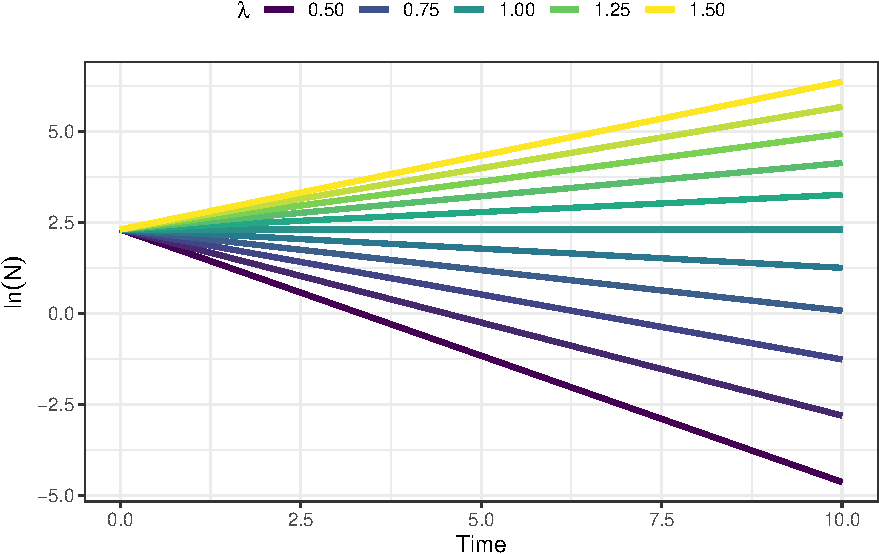
\includegraphics{DemographyCompendium_files/figure-latex/unnamed-chunk-42-1.pdf}

\hypertarget{exercise-1.2-1}{%
\subsection*{Exercise 1.2}\label{exercise-1.2-1}}
\addcontentsline{toc}{subsection}{Exercise 1.2}

\begin{enumerate}
\def\labelenumi{\arabic{enumi}.}
\item
  Value of \(\lambda\): If the population grows by 1\(\%\) per day, that means \(\lambda\approx 1.01\), with a unit of days.
\item
  Doubling time: We denote the doubling time as \(t_2\). Inserting \(N=2N_0\) in the equation of exponential growth, we get:
\end{enumerate}

\begin{align*}
2N_0&=N_0\lambda^{t_2}\\ 
\lambda^{t_2}&=2 \\ t_2\ln\lambda&=2\\ 
t_2&=\frac{2}{\ln\lambda} =\frac{2}{\ln 1.01} \approx 201.  
\end{align*}

Thus, the population will take approximately 201 days to double in size.

\begin{enumerate}
\def\labelenumi{\arabic{enumi}.}
\setcounter{enumi}{2}
\tightlist
\item
  Population size after 1 year: One year is approximately 365 days, so with a starting populatoin of 100 individuals we get
\end{enumerate}

\[N=100\cdot 1.01^{365}\approx 3778.\]
Plot population growth over a year:

\begin{Shaded}
\begin{Highlighting}[]
\NormalTok{sgrowth }\OtherTok{\textless{}{-}} \FunctionTok{Exp.growth}\NormalTok{(}\AttributeTok{lambda=}\FloatTok{1.01}\NormalTok{, }\AttributeTok{N0=}\DecValTok{100}\NormalTok{, }\AttributeTok{Tmax=}\DecValTok{365}\NormalTok{)}

\CommentTok{\#Store as data frame for plotting:}
\NormalTok{silverfish }\OtherTok{\textless{}{-}} \FunctionTok{data.frame}\NormalTok{(sgrowth, }\AttributeTok{Time=}\DecValTok{0}\SpecialCharTok{:}\DecValTok{365}\NormalTok{)}

\CommentTok{\#Plot with ggplot:}
\FunctionTok{ggplot}\NormalTok{(silverfish) }\SpecialCharTok{+} 
    \FunctionTok{geom\_line}\NormalTok{(}\FunctionTok{aes}\NormalTok{(}\AttributeTok{x=}\NormalTok{Time, }\AttributeTok{y=}\NormalTok{sgrowth), }\AttributeTok{lwd=}\FloatTok{1.2}\NormalTok{) }\SpecialCharTok{+}
    \FunctionTok{theme\_bw}\NormalTok{() }\SpecialCharTok{+}
    \FunctionTok{labs}\NormalTok{( }\AttributeTok{x=}\StringTok{"Time"}\NormalTok{, }\AttributeTok{y=}\StringTok{"Silverfish population"}\NormalTok{)}
\end{Highlighting}
\end{Shaded}

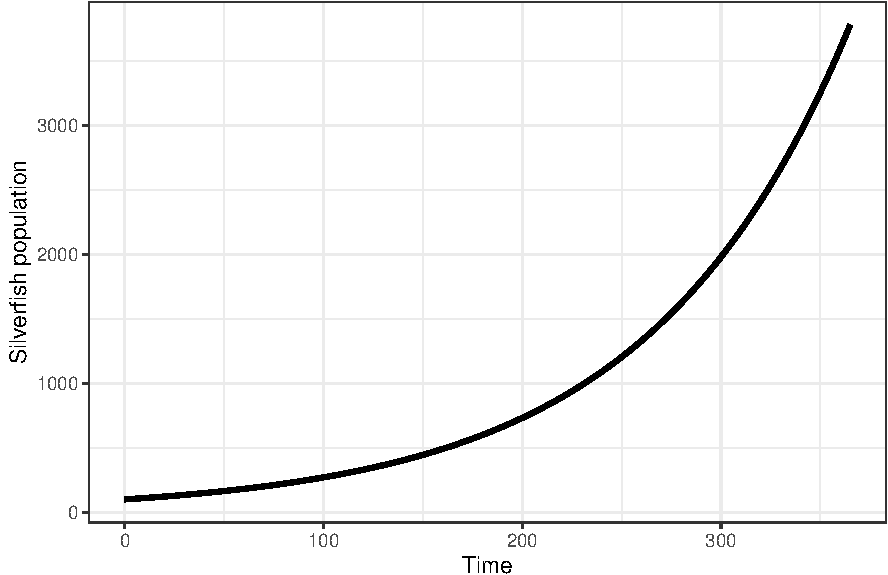
\includegraphics{DemographyCompendium_files/figure-latex/unnamed-chunk-43-1.pdf}

\hypertarget{chapter-2-exercises}{%
\section{Chapter 2 exercises}\label{chapter-2-exercises}}

\hypertarget{exercise-2.1-1}{%
\subsection*{Exercise 2.1}\label{exercise-2.1-1}}
\addcontentsline{toc}{subsection}{Exercise 2.1}

\begin{enumerate}
\def\labelenumi{\arabic{enumi}.}
\tightlist
\item
  The number of children includes boys and girls, so to get \(R_0\) we divide by half (assuming equal sex ratio at birth). Using the approximation (\(\lambda\approx \exp\left(\frac{\ln R_0}{T_C}\right)\)), we can add values of \(\lambda\) to the table (here assuming a generatio ntime of \(T_C=25\) or \(T_C=30\)):
\end{enumerate}

\begin{tabular}{ccccc}
\toprule
Country & Children per woman & $R_0$ & $\lambda_{25}$ & $\lambda_{30}$\\
\midrule
Mali & 5.8 & 2.90 & 1.044 & 1.036\\
Tunisia & 2.2 & 1.10 & 1.004 & 1.003\\
Australia & 1.7 & 0.85 & 0.994 & 0.995\\
Norway & 1.6 & 0.80 & 0.991 & 0.993\\
South Korea & 0.9 & 0.45 & 0.969 & 0.974\\
\bottomrule
\end{tabular}

As generation time \(T_C\) increases, \(\lambda\) increases if the population is declining (\(\lambda<1\)), but declines if the population is growing (note: this exercise ignores immigration and emigration so the value of \(\lambda\) does not represent the real population trends in these countries.)

\begin{enumerate}
\def\labelenumi{\arabic{enumi}.}
\setcounter{enumi}{1}
\tightlist
\item
  To answer this question we use the values \(\lambda_{25}\), and apply the formula from exercise 1.2 to find the doubling time (\(t_{2}=2/\ln \lambda_{25}\)):
\end{enumerate}

\begin{tabular}{ccccc}
\toprule
Country & Children per woman & $R_0$ & $\lambda_{25}$ & Doubling time\\
\midrule
Mali & 5.8 & 2.90 & 1.044 & 46.961\\
Tunisia & 2.2 & 1.10 & 1.004 & 524.603\\
Australia & 1.7 & 0.85 & 0.994 & -307.656\\
Norway & 1.6 & 0.80 & 0.991 & -224.071\\
South Korea & 0.9 & 0.45 & 0.969 & -62.617\\
\bottomrule
\end{tabular}

Declining populations (\(\lambda<1\)) get negative doubling rates. Naturally these populations cannot double in size with negative growth. The growing populations (\(\lambda>1\)) have a doubling time of 47 years (Mali) and 525 years (Tunisia).

\begin{enumerate}
\def\labelenumi{\arabic{enumi}.}
\setcounter{enumi}{2}
\tightlist
\item
  The exponential growth model is too simple to describe long-term growth of human population sizes. It describes current trends of growth given the current rates of survival and fertility. Both survival and fertility change over time, and the annual population growth rate is not constant, but has declined over time in most countries. The generation time also varies much among populations and will change over time (as it is a function of the survival and fertility rates). In particular for countries that currently grow fast we should be careful with making long-term extrapolations based on the exponential growth model. Finally, this exercise ignores immigration and emigration, which can be a large factor affecting population growth.
\end{enumerate}

\hypertarget{exercise-2.2-1}{%
\subsection*{Exercise 2.2}\label{exercise-2.2-1}}
\addcontentsline{toc}{subsection}{Exercise 2.2}

\begin{enumerate}
\def\labelenumi{\arabic{enumi}.}
\item
  The age at first reproduction is 3 years. This is the first age where \(m_x>0\) in the life table.
\item
  Creating the life table in R (here we use the function ´data.frame()´, other options can also be used, like \texttt{tibble()} from tidyverse):
\end{enumerate}

\begin{Shaded}
\begin{Highlighting}[]
\NormalTok{x }\OtherTok{\textless{}{-}} \DecValTok{0}\SpecialCharTok{:}\DecValTok{4} 
\NormalTok{nx }\OtherTok{\textless{}{-}} \FunctionTok{c}\NormalTok{(}\DecValTok{12376}\NormalTok{, }\DecValTok{4233}\NormalTok{, }\DecValTok{1790}\NormalTok{, }\DecValTok{340}\NormalTok{, }\DecValTok{268}\NormalTok{)}
\NormalTok{mx }\OtherTok{\textless{}{-}} \FunctionTok{c}\NormalTok{(}\DecValTok{0}\NormalTok{, }\DecValTok{0}\NormalTok{, }\DecValTok{0}\NormalTok{, }\FloatTok{2.1}\NormalTok{, }\FloatTok{3.2}\NormalTok{)}
 
\NormalTok{PlantTable }\OtherTok{\textless{}{-}} \FunctionTok{data.frame}\NormalTok{(x, nx, mx) }
\end{Highlighting}
\end{Shaded}

\begin{enumerate}
\def\labelenumi{\arabic{enumi}.}
\setcounter{enumi}{2}
\tightlist
\item
  Adding vectors of cumulative survival probability \(l_x\) and annual survival probability \(p_x\) to the life table:
\end{enumerate}

\begin{Shaded}
\begin{Highlighting}[]
\NormalTok{lx }\OtherTok{\textless{}{-}}\NormalTok{ nx}\SpecialCharTok{/}\NormalTok{nx[}\DecValTok{1}\NormalTok{] }\CommentTok{\#divide all elements of nx by the first.}
\NormalTok{px }\OtherTok{\textless{}{-}} \FunctionTok{c}\NormalTok{(lx[}\DecValTok{2}\SpecialCharTok{:}\DecValTok{5}\NormalTok{]}\SpecialCharTok{/}\NormalTok{lx[}\DecValTok{1}\SpecialCharTok{:}\DecValTok{4}\NormalTok{],}\DecValTok{0}\NormalTok{) }\CommentTok{\#by definition the last value is zero.}

\NormalTok{PlantTable}\SpecialCharTok{$}\NormalTok{lx }\OtherTok{\textless{}{-}}\NormalTok{ lx}
\NormalTok{PlantTable}\SpecialCharTok{$}\NormalTok{px }\OtherTok{\textless{}{-}}\NormalTok{ px}

\NormalTok{PlantTable}
\end{Highlighting}
\end{Shaded}

\begin{verbatim}
##   x    nx  mx         lx        px
## 1 0 12376 0.0 1.00000000 0.3420330
## 2 1  4233 0.0 0.34203297 0.4228679
## 3 2  1790 0.0 0.14463478 0.1899441
## 4 3   340 2.1 0.02747253 0.7882353
## 5 4   268 3.2 0.02165482 0.0000000
\end{verbatim}

\begin{enumerate}
\def\labelenumi{\arabic{enumi}.}
\setcounter{enumi}{3}
\tightlist
\item
  Plots of each life table column (\(n_x\), \(l_x\), \(p_x\), \(m_x\)) as a function of age \(x\):
\end{enumerate}

\begin{Shaded}
\begin{Highlighting}[]
\CommentTok{\#Convert to long table format for plotting:}
\NormalTok{plant.long }\OtherTok{\textless{}{-}}\NormalTok{ PlantTable }\SpecialCharTok{\%\textgreater{}\%} \FunctionTok{pivot\_longer}\NormalTok{(}\FunctionTok{c}\NormalTok{(nx,lx, px,  mx),}
               \AttributeTok{names\_to =} \StringTok{"VitalRates"}\NormalTok{, }\AttributeTok{values\_to =} \StringTok{"Value"}\NormalTok{)}
 
\FunctionTok{ggplot}\NormalTok{(plant.long) }\SpecialCharTok{+} 
  \FunctionTok{geom\_line}\NormalTok{(}\FunctionTok{aes}\NormalTok{(}\AttributeTok{x=}\NormalTok{x, }\AttributeTok{y=}\NormalTok{Value ),}\AttributeTok{col=}\DecValTok{1}\NormalTok{, }\AttributeTok{lwd=}\FloatTok{1.2}\NormalTok{)}\SpecialCharTok{+}
  \FunctionTok{facet\_wrap}\NormalTok{(}\SpecialCharTok{\textasciitilde{}}\FunctionTok{factor}\NormalTok{(VitalRates,}\AttributeTok{levels=}\FunctionTok{c}\NormalTok{(}\StringTok{"nx"}\NormalTok{, }\StringTok{"lx"}\NormalTok{ , }\StringTok{"px"}\NormalTok{, }\StringTok{"mx"}\NormalTok{)), }\AttributeTok{scales=}\StringTok{"free"}\NormalTok{)}\SpecialCharTok{+}
  \FunctionTok{theme\_bw}\NormalTok{() }\SpecialCharTok{+}
  \FunctionTok{labs}\NormalTok{( }\AttributeTok{x=}\StringTok{"Age (year)"}\NormalTok{, }\AttributeTok{y=}\StringTok{"Value"}\NormalTok{)}
\end{Highlighting}
\end{Shaded}

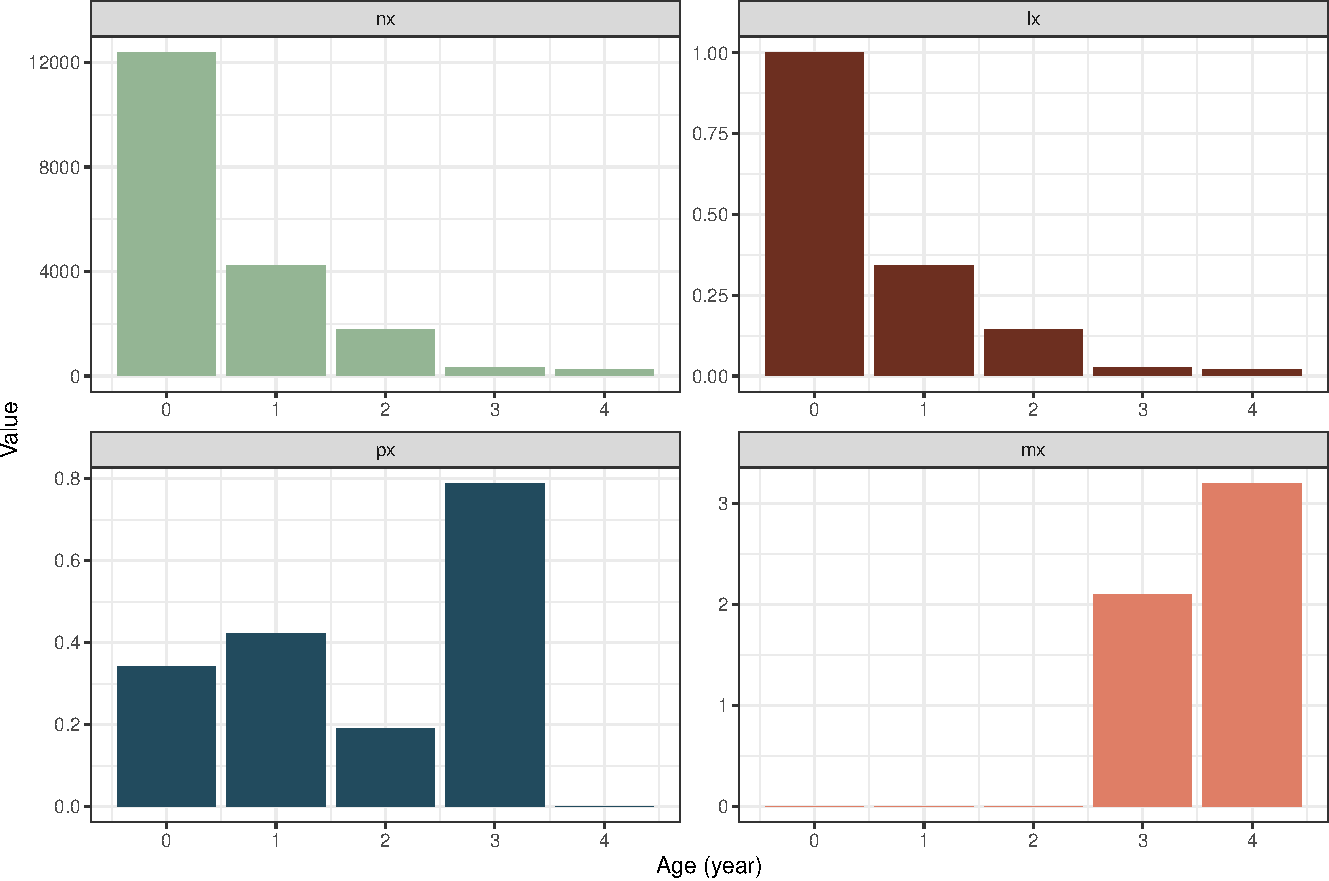
\includegraphics{DemographyCompendium_files/figure-latex/unnamed-chunk-46-1.pdf}

The shape of \(l_x\) follows the decline in cohort size over age, as it should. The annual survival probability fluctuates between ages but is quite low in the first years until the plant starts to reproduce at age 3. From age 3 to 4 the survival probability is much higher, almost 0.8, but then no plants survive after age 4 (last reproduction). Since all remaining plants die in the final year, the plants likely invest all resources in reproduction this year, and fecundity is higher at the second reproduction.

\begin{enumerate}
\def\labelenumi{\arabic{enumi}.}
\setcounter{enumi}{4}
\tightlist
\item
  Mean lifetime reproduction \(R_0\) from the life table:
\end{enumerate}

\begin{Shaded}
\begin{Highlighting}[]
\NormalTok{R0\_Plant }\OtherTok{\textless{}{-}} \FunctionTok{sum}\NormalTok{(PlantTable}\SpecialCharTok{$}\NormalTok{lx}\SpecialCharTok{*}\NormalTok{PlantTable}\SpecialCharTok{$}\NormalTok{mx)}

\FunctionTok{round}\NormalTok{(R0\_Plant, }\AttributeTok{digits=}\DecValTok{3}\NormalTok{)}
\end{Highlighting}
\end{Shaded}

\begin{verbatim}
## [1] 0.127
\end{verbatim}

The value of \(R_0\) is very low. Each plant is replaced by only 0.13 new plants on average. This means that \(\lambda<1\).

\begin{enumerate}
\def\labelenumi{\arabic{enumi}.}
\setcounter{enumi}{5}
\tightlist
\item
  Generation time \(T_C\) from the life table:
\end{enumerate}

\begin{Shaded}
\begin{Highlighting}[]
\NormalTok{TC\_Plant }\OtherTok{\textless{}{-}} \FunctionTok{sum}\NormalTok{(PlantTable}\SpecialCharTok{$}\NormalTok{x}\SpecialCharTok{*}\NormalTok{PlantTable}\SpecialCharTok{$}\NormalTok{lx}\SpecialCharTok{*}\NormalTok{PlantTable}\SpecialCharTok{$}\NormalTok{mx)}\SpecialCharTok{/}\NormalTok{R0\_Plant}

\FunctionTok{round}\NormalTok{(TC\_Plant, }\AttributeTok{digits=}\DecValTok{3}\NormalTok{)}
\end{Highlighting}
\end{Shaded}

\begin{verbatim}
## [1] 3.546
\end{verbatim}

This is the cohort generation time, and shows the average age at which the \(R_0\) offspring are produced.

Approximation of \(\lambda\) based on \(R_0\) and \(T_C\):

\begin{Shaded}
\begin{Highlighting}[]
\NormalTok{lambda\_Plant }\OtherTok{\textless{}{-}} \FunctionTok{exp}\NormalTok{(}\FunctionTok{log}\NormalTok{(R0\_Plant)}\SpecialCharTok{/}\NormalTok{TC\_Plant)}

\FunctionTok{round}\NormalTok{(lambda\_Plant, }\AttributeTok{digits=}\DecValTok{3}\NormalTok{)}
\end{Highlighting}
\end{Shaded}

\begin{verbatim}
## [1] 0.559
\end{verbatim}

Thus, the population growth rate is very low at \(\lambda\approx\) 0.559. Almost half the population is lost each year.

\begin{enumerate}
\def\labelenumi{\arabic{enumi}.}
\setcounter{enumi}{6}
\tightlist
\item
  Solving the Euler-Lotka equation for \(\lambda\):
\end{enumerate}

\begin{Shaded}
\begin{Highlighting}[]
\CommentTok{\#Rearranging the Euler{-}Lotka function to get an expression equal to zero:}
\NormalTok{EulerLotka }\OtherTok{\textless{}{-}} \ControlFlowTok{function}\NormalTok{(lambda, x, lx, mx)\{}
  \FunctionTok{sum}\NormalTok{(lambda}\SpecialCharTok{\^{}}\NormalTok{(}\SpecialCharTok{{-}}\NormalTok{x)}\SpecialCharTok{*}\NormalTok{lx}\SpecialCharTok{*}\NormalTok{mx)}\SpecialCharTok{{-}}\DecValTok{1}
\NormalTok{\}}

\CommentTok{\#Define search range for lambda in uniroot}
\NormalTok{lambda.range }\OtherTok{\textless{}{-}} \FunctionTok{c}\NormalTok{(.}\DecValTok{1}\NormalTok{,}\DecValTok{2}\NormalTok{)}

\CommentTok{\#Apply uniroot to find lambda, store the result}
\NormalTok{lambda\_Plant2 }\OtherTok{\textless{}{-}} \FunctionTok{uniroot}\NormalTok{(EulerLotka, }\AttributeTok{x=}\NormalTok{PlantTable}\SpecialCharTok{$}\NormalTok{x, }\AttributeTok{lx=}\NormalTok{PlantTable}\SpecialCharTok{$}\NormalTok{lx, }\AttributeTok{mx=}\NormalTok{PlantTable}\SpecialCharTok{$}\NormalTok{mx, }\AttributeTok{interval=}\NormalTok{lambda.range)}\SpecialCharTok{$}\NormalTok{root}

\FunctionTok{round}\NormalTok{(lambda\_Plant2, }\AttributeTok{digits=}\DecValTok{3}\NormalTok{)}
\end{Highlighting}
\end{Shaded}

\begin{verbatim}
## [1] 0.565
\end{verbatim}

The value calculated from the Euler-Lotka equation is \(\lambda\approx\) 0.565, a bit higher than the approximated value.

\hypertarget{exercise-2.3-1}{%
\subsection*{Exercise 2.3}\label{exercise-2.3-1}}
\addcontentsline{toc}{subsection}{Exercise 2.3}

\begin{enumerate}
\def\labelenumi{\arabic{enumi}.}
\tightlist
\item
  According to table \ref{tab:tablebird}, the fecundity values of age 2 and 3 are \(m_2=3\) and \(m_3=6\). To get the clutch size these values should be multiplied by 2 (assuming equal sex ratio), and divided by the survival probability. This gives an average clutch size of \(M_2=3\cdot2/0.9=6.67\) eggs at age 3, and \(M_2=6\cdot2/0.9=13.33\) eggs at age 4.
\end{enumerate}

Thus, older parents produce larger clutches than younger ones, in this (fictive) example.

\begin{enumerate}
\def\labelenumi{\arabic{enumi}.}
\setcounter{enumi}{1}
\item
  Under the assumptions of the Lack clutch, the trade-off is defined as \(c=\frac{1}{2N_e^*}\). At age 2, the Lack clutch size is 6.67 and we thus get \(c=\frac{1}{2\cdot6.67}\approx 0.074\). At age 3 the Lack clutch size is 13.33 and the trade-off is \(c=\frac{1}{2\cdot13.33}\approx 0.038\). Remember that the stronger the trade-off, the lower the clutch size. If the clutch size at each age is determined by this trade-off only (as the Lack clutch assumes), this means that the trade-off is reduced with age for this example. In reality, physical and behavioral constraints also limit clutch size of young versus older birds, in particular in first-time breeders versus experienced breeders.
\item
  To solve this we use the Euler-Lotka-equation, and insert the information we have (the value of \(\lambda=1.07\) is calculated in the example for the Euler-Lotka equation):
\end{enumerate}

\begin{align*}
\sum_x \lambda^{-x}l_xm_x&=1\\
\lambda^{-3}l_3m_3&=1\\
1.07^{-3}0.108m_3&=1\\
m_3&=1.07^{3}/0.108 \approx 11.34.
\end{align*}

Thus, the fecundity of the related species is higher, which makes sense since it only reproduces at age 3 while still having the same fitness as the example bird.

\begin{enumerate}
\def\labelenumi{\arabic{enumi}.}
\setcounter{enumi}{4}
\tightlist
\item
  In Cole's paradox, the semelparous species only needs one more offspring per clutch to get the same fitness as the iteroparous species. The result of the previous question tells us that the semelparous bird needs a much larger clutch size to match the fitness of the iteroparous species (or example species), so clearly semelparity is not as `cheap' here as in Cole's example.
\end{enumerate}

Cole assumed a survival probability of 1 for the iteroparous species, and that both species reproduced from year 1, neither of which apply to the two bird species here. In both species there is a difference between juveniles and adults (juveniles do not reproduce), also not fitting the assumptions in Cole's paradox.

\hypertarget{chapter-3-exercises}{%
\section{Chapter 3 exercises}\label{chapter-3-exercises}}

\hypertarget{exercise-3.1-1}{%
\subsection*{Exercise 3.1}\label{exercise-3.1-1}}
\addcontentsline{toc}{subsection}{Exercise 3.1}

Life cycle for the bird example, with post-reproductive census:

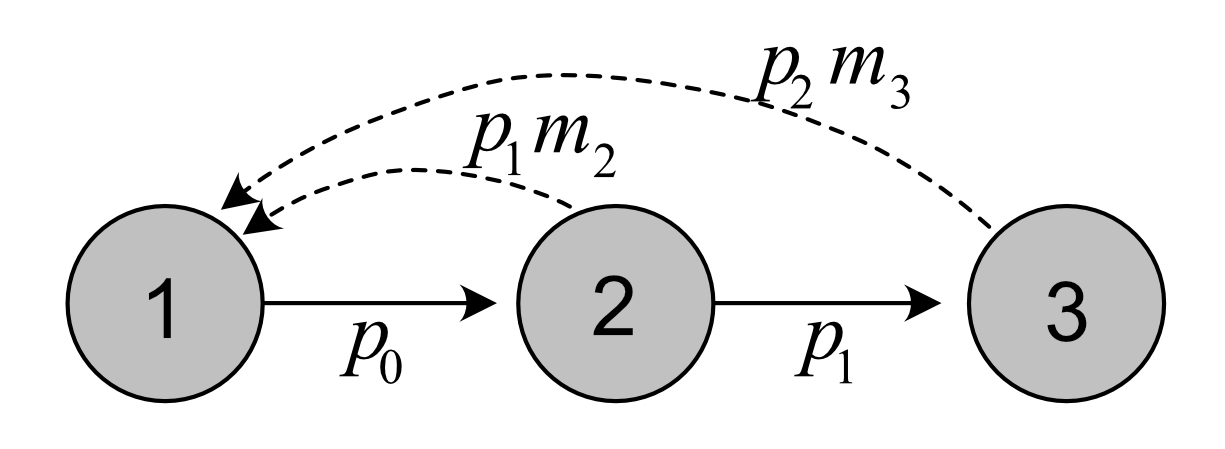
\includegraphics[width=0.6\linewidth]{LifeCycleAgePost}

Note that each age class is numbered from 1 to 3, although they correspond to actual age 0 to 2 in this case.

\hypertarget{exercise-3.2-1}{%
\subsection*{Exercise 3.2}\label{exercise-3.2-1}}
\addcontentsline{toc}{subsection}{Exercise 3.2}

\hypertarget{pre-reproductive-census-1}{%
\subsubsection*{Pre-reproductive census:}\label{pre-reproductive-census-1}}
\addcontentsline{toc}{subsubsection}{Pre-reproductive census:}

\begin{enumerate}
\def\labelenumi{\arabic{enumi}.}
\tightlist
\item
  Life cycle graph of plant:
\end{enumerate}

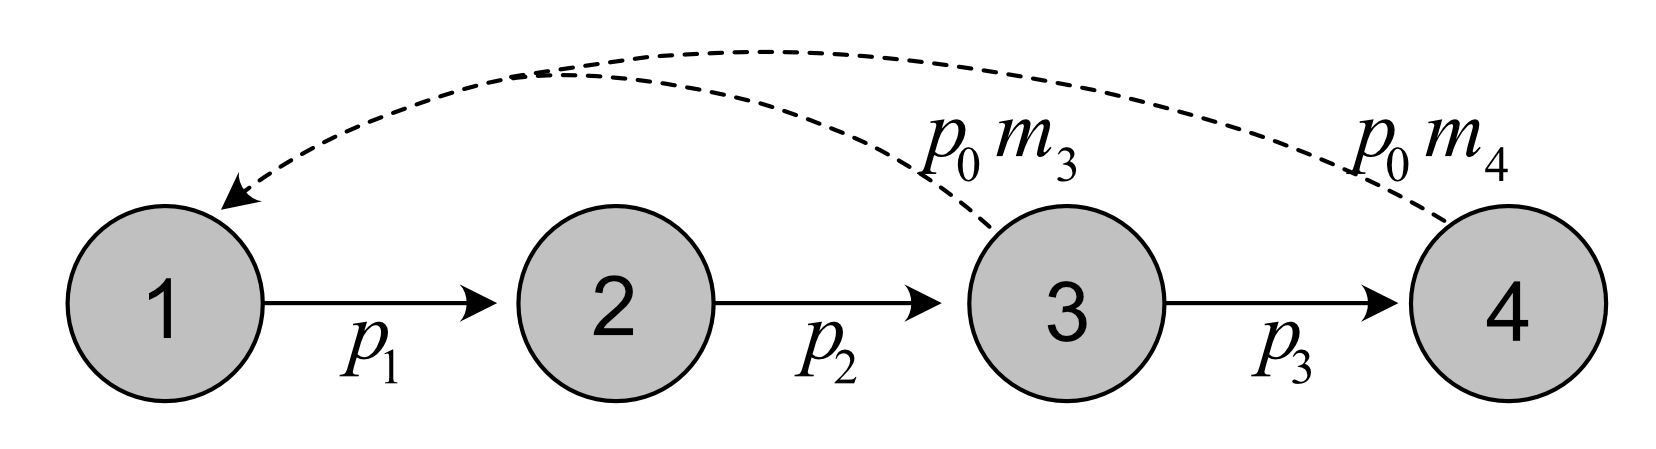
\includegraphics[width=0.6\linewidth]{LifeCyclePlantPRE}

\begin{enumerate}
\def\labelenumi{\arabic{enumi}.}
\setcounter{enumi}{1}
\tightlist
\item
  Vectors of fertility and survival coefficients:
\end{enumerate}

\begin{Shaded}
\begin{Highlighting}[]
\NormalTok{px }\OtherTok{\textless{}{-}}\NormalTok{ PlantTable}\SpecialCharTok{$}\NormalTok{px}
\NormalTok{mx }\OtherTok{\textless{}{-}}\NormalTok{ PlantTable}\SpecialCharTok{$}\NormalTok{mx}

\NormalTok{fertility.plant }\OtherTok{\textless{}{-}}\NormalTok{ px[}\DecValTok{1}\NormalTok{]}\SpecialCharTok{*}\NormalTok{mx[}\DecValTok{2}\SpecialCharTok{:}\DecValTok{5}\NormalTok{] }\CommentTok{\#corresponding to age class 1:4}
\NormalTok{survival.plant }\OtherTok{\textless{}{-}}\NormalTok{ px[}\DecValTok{2}\SpecialCharTok{:}\DecValTok{5}\NormalTok{] }\CommentTok{\#corresponding to age class 1:4}
\end{Highlighting}
\end{Shaded}

\begin{enumerate}
\def\labelenumi{\arabic{enumi}.}
\setcounter{enumi}{2}
\tightlist
\item
  Define \(\mathbf{A}\), \(\mathbf{U}\) and \(\mathbf{F}\):
\end{enumerate}

\begin{Shaded}
\begin{Highlighting}[]
\NormalTok{AmatPlant }\OtherTok{\textless{}{-}} \FunctionTok{Create.Amat}\NormalTok{(}\AttributeTok{Svec=}\NormalTok{survival.plant, }\AttributeTok{Fvec=}\NormalTok{fertility.plant)}
\NormalTok{FmatPlant }\OtherTok{\textless{}{-}}\NormalTok{ UmatPlant }\OtherTok{\textless{}{-}}\NormalTok{ AmatPlant}

\NormalTok{FmatPlant[}\SpecialCharTok{{-}}\DecValTok{1}\NormalTok{,] }\OtherTok{\textless{}{-}} \DecValTok{0} \CommentTok{\#Set all elements to zero that are not on the first row}
\NormalTok{UmatPlant[}\DecValTok{1}\NormalTok{,] }\OtherTok{\textless{}{-}} \DecValTok{0} \CommentTok{\#Set all elements to zero in the first row}

\NormalTok{AmatPlant}
\end{Highlighting}
\end{Shaded}

\begin{verbatim}
##           [,1]      [,2]      [,3]     [,4]
## [1,] 0.0000000 0.0000000 0.7182692 1.094505
## [2,] 0.4228679 0.0000000 0.0000000 0.000000
## [3,] 0.0000000 0.1899441 0.0000000 0.000000
## [4,] 0.0000000 0.0000000 0.7882353 0.000000
\end{verbatim}

\begin{enumerate}
\def\labelenumi{\arabic{enumi}.}
\setcounter{enumi}{3}
\tightlist
\item
  Project age classes over 30 time steps:
\end{enumerate}

\begin{Shaded}
\begin{Highlighting}[]
\CommentTok{\#Return matrix of projected growth of each age class over time:}
\NormalTok{Pop.plant }\OtherTok{\textless{}{-}} \FunctionTok{projection}\NormalTok{(}\AttributeTok{MatA=}\NormalTok{AmatPlant, }\AttributeTok{n0=}\FunctionTok{rep}\NormalTok{(}\DecValTok{10}\NormalTok{, }\DecValTok{4}\NormalTok{), }\AttributeTok{Tmax=}\DecValTok{30}\NormalTok{)}
 
\CommentTok{\#Long format for plotting:}
\NormalTok{Pop.plant.long }\OtherTok{\textless{}{-}}\NormalTok{ Pop.plant }\SpecialCharTok{\%\textgreater{}\%} \FunctionTok{pivot\_longer}\NormalTok{(}\FunctionTok{c}\NormalTok{(}\SpecialCharTok{{-}}\NormalTok{time),}
               \AttributeTok{names\_to =} \StringTok{"AgeClass"}\NormalTok{, }\AttributeTok{values\_to =} \StringTok{"Value"}\NormalTok{)}

\CommentTok{\#Plot}
\FunctionTok{ggplot}\NormalTok{(Pop.plant.long) }\SpecialCharTok{+} 
  \FunctionTok{geom\_line}\NormalTok{(}\FunctionTok{aes}\NormalTok{(}\AttributeTok{x=}\NormalTok{time,}\AttributeTok{y=}\NormalTok{Value, }\AttributeTok{col=}\NormalTok{AgeClass, }\AttributeTok{linetype=}\NormalTok{AgeClass), }\AttributeTok{lwd=}\FloatTok{1.2}\NormalTok{)}\SpecialCharTok{+}
  \FunctionTok{theme\_bw}\NormalTok{() }\SpecialCharTok{+}
  \FunctionTok{scale\_color\_manual}\NormalTok{(}\AttributeTok{values=}\FunctionTok{c}\NormalTok{(}\DecValTok{1}\NormalTok{,}\DecValTok{2}\NormalTok{,}\DecValTok{3}\NormalTok{,}\DecValTok{4}\NormalTok{))}\SpecialCharTok{+} \CommentTok{\#Add colors manually}
  \FunctionTok{scale\_linetype\_manual}\NormalTok{(}\AttributeTok{values=}\FunctionTok{c}\NormalTok{(}\DecValTok{1}\NormalTok{,}\DecValTok{2}\NormalTok{,}\DecValTok{3}\NormalTok{,}\DecValTok{4}\NormalTok{))}\SpecialCharTok{+} \CommentTok{\#Add linetypes manually}
  \FunctionTok{labs}\NormalTok{( }\AttributeTok{x=}\StringTok{"Time (year)"}\NormalTok{, }\AttributeTok{y=}\StringTok{"Age class size"}\NormalTok{)}\SpecialCharTok{+} \CommentTok{\#Axis labels}
  \FunctionTok{theme}\NormalTok{(}\AttributeTok{legend.position =} \StringTok{"top"}\NormalTok{ ) }\CommentTok{\#Place legend on top}
\end{Highlighting}
\end{Shaded}

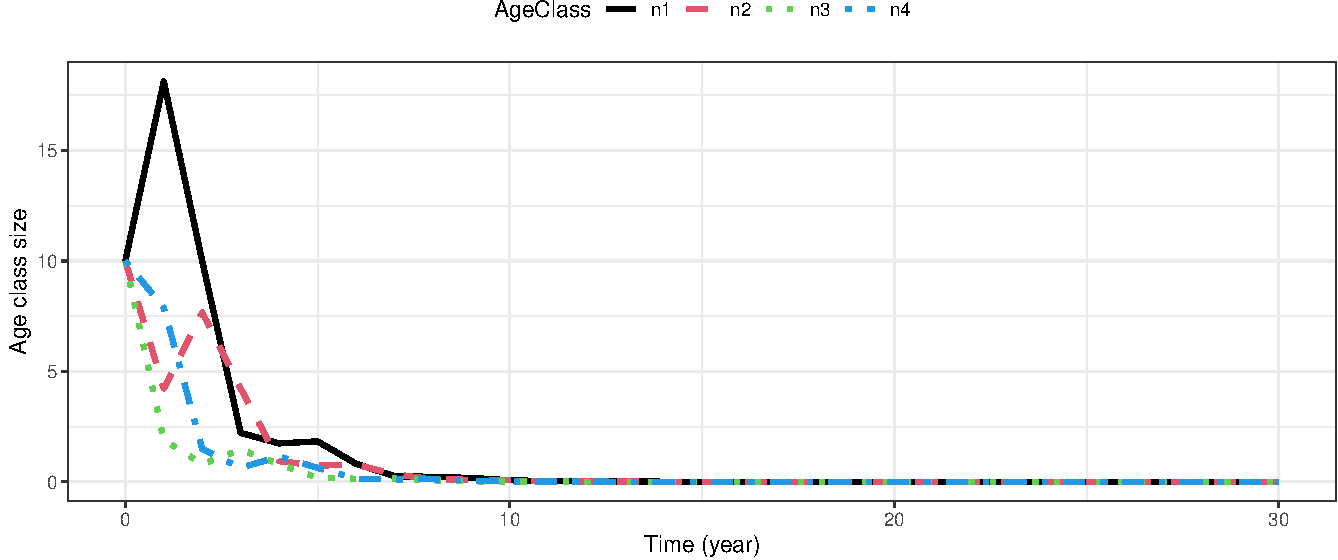
\includegraphics{DemographyCompendium_files/figure-latex/unnamed-chunk-55-1.pdf}

\begin{enumerate}
\def\labelenumi{\arabic{enumi}.}
\setcounter{enumi}{4}
\tightlist
\item
  Calculate \(\lambda\), \(R_0\) and \(G\) using the matrices:
\end{enumerate}

\begin{Shaded}
\begin{Highlighting}[]
\NormalTok{res.plant }\OtherTok{\textless{}{-}} \FunctionTok{uvlambda}\NormalTok{(AmatPlant)}
\NormalTok{lambda.plant }\OtherTok{\textless{}{-}}\NormalTok{ res.plant}\SpecialCharTok{$}\NormalTok{lambda}
\NormalTok{R0.plant }\OtherTok{\textless{}{-}} \FunctionTok{R0function}\NormalTok{(UmatPlant, FmatPlant)}\SpecialCharTok{$}\NormalTok{R0}
\NormalTok{G.plant }\OtherTok{\textless{}{-}} \FunctionTok{GenTime}\NormalTok{(AmatPlant, FmatPlant)}

\NormalTok{ResVec }\OtherTok{\textless{}{-}} \FunctionTok{c}\NormalTok{(lambda.plant, R0.plant, G.plant) }\CommentTok{\#Store results}
\FunctionTok{names}\NormalTok{(ResVec) }\OtherTok{\textless{}{-}} \FunctionTok{c}\NormalTok{(}\StringTok{"lambda"}\NormalTok{, }\StringTok{"R0"}\NormalTok{, }\StringTok{"G"}\NormalTok{)}
\FunctionTok{round}\NormalTok{(ResVec,}\DecValTok{3}\NormalTok{)}
\end{Highlighting}
\end{Shaded}

\begin{verbatim}
## lambda     R0      G 
##  0.565  0.127  3.680
\end{verbatim}

These are approximately the same values as found from the life table. The generation time is slightly different because it is not the same measure. For the life table calculations we used the cohort generation time, while for the matrix model we used the mean age of mothers at the stable distribution.

\begin{enumerate}
\def\labelenumi{\arabic{enumi}.}
\setcounter{enumi}{5}
\tightlist
\item
  Calculate and plot \(\mathbf{u}\) and \(\mathbf{v}\):
\end{enumerate}

These values were calculated in the previous point using the R function \texttt{uvlambda()}. To plot them:

\begin{Shaded}
\begin{Highlighting}[]
\CommentTok{\#Create data frame for plotting}
\NormalTok{plantframe }\OtherTok{\textless{}{-}} \FunctionTok{data.frame}\NormalTok{(}\StringTok{"AgeClass"}\OtherTok{=}\FunctionTok{factor}\NormalTok{(}\DecValTok{1}\SpecialCharTok{:}\DecValTok{4}\NormalTok{), }\StringTok{"u"}\OtherTok{=}\NormalTok{res.plant}\SpecialCharTok{$}\NormalTok{u, }\StringTok{"v"}\OtherTok{=}\FunctionTok{t}\NormalTok{(res.plant}\SpecialCharTok{$}\NormalTok{v))}

\CommentTok{\#Long format for plotting:}
\NormalTok{plantframe.long }\OtherTok{\textless{}{-}}\NormalTok{ plantframe }\SpecialCharTok{\%\textgreater{}\%} \FunctionTok{pivot\_longer}\NormalTok{(}\FunctionTok{c}\NormalTok{(u,v),}
               \AttributeTok{names\_to =} \StringTok{"Vector"}\NormalTok{, }\AttributeTok{values\_to =} \StringTok{"Value"}\NormalTok{)}

 
\CommentTok{\#Plot}
\FunctionTok{ggplot}\NormalTok{(plantframe.long) }\SpecialCharTok{+} 
  \FunctionTok{geom\_col}\NormalTok{(}\FunctionTok{aes}\NormalTok{(}\AttributeTok{x=}\NormalTok{AgeClass, }\AttributeTok{y=}\NormalTok{Value, }\AttributeTok{fill=}\NormalTok{AgeClass ), }\AttributeTok{lwd=}\FloatTok{1.2}\NormalTok{)}\SpecialCharTok{+}
  \FunctionTok{theme\_bw}\NormalTok{() }\SpecialCharTok{+}
  \FunctionTok{facet\_wrap}\NormalTok{(}\FunctionTok{vars}\NormalTok{(Vector),}\AttributeTok{ncol=}\DecValTok{2}\NormalTok{,}\AttributeTok{scales=}\StringTok{"free"}\NormalTok{)}\SpecialCharTok{+}
  \FunctionTok{scale\_fill\_manual}\NormalTok{(}\AttributeTok{values=}\NormalTok{colors4)}\SpecialCharTok{+} \CommentTok{\#Add colors manually}
  \FunctionTok{labs}\NormalTok{( }\AttributeTok{x=}\StringTok{"Age class"}\NormalTok{, }\AttributeTok{y=}\StringTok{"Value"}\NormalTok{)}\SpecialCharTok{+} \CommentTok{\#Axis labels}
  \FunctionTok{theme}\NormalTok{(}\AttributeTok{legend.position =} \StringTok{"none"}\NormalTok{ ) }\CommentTok{\#Drop legend}
\end{Highlighting}
\end{Shaded}

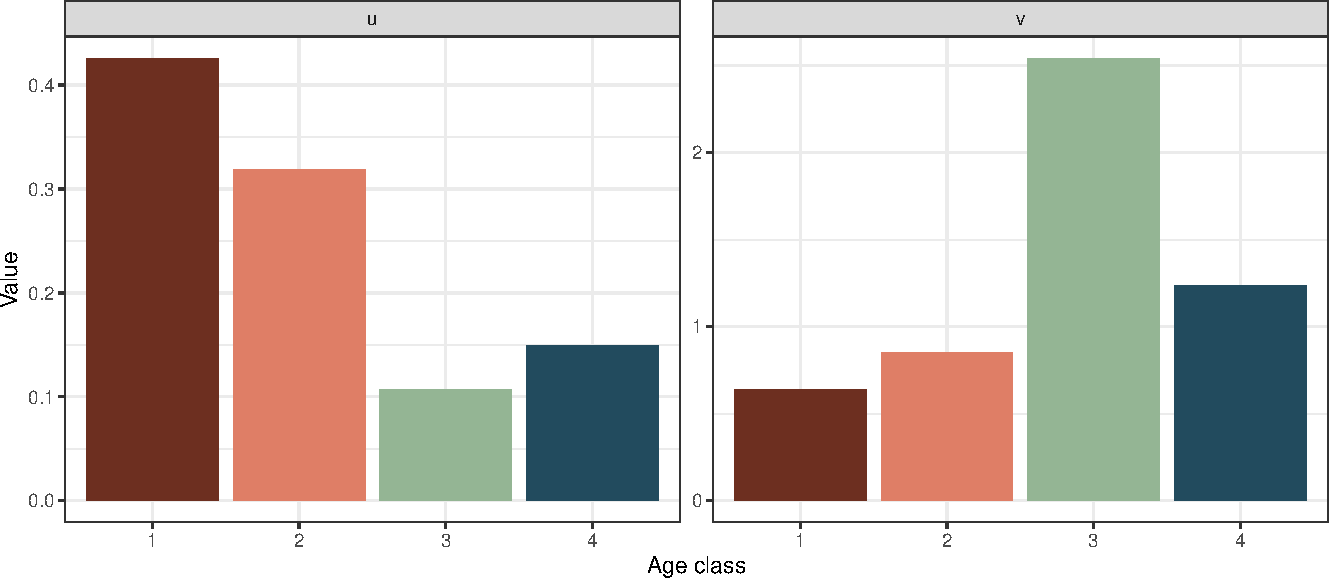
\includegraphics{DemographyCompendium_files/figure-latex/unnamed-chunk-57-1.pdf}

The stable age structure tells us the proportion of individuals in each age class when the population has reached the stable growth phase. In this case the stable age structure shows a higher proportion of individuals in age class 4 than in age class 3. This is uncommon for age structured populations (usually the stable age structure declines with age), and is due to the extremely low value of \(\lambda\).

The reproductive values tell us how much individuals in each age class will contribute to the future population, relative to other age classes (when the population has reached the stable growth phase). In this case the reproductive value is highest in age class 3, followed by age class 4, the two reproductive classes.

\begin{enumerate}
\def\labelenumi{\arabic{enumi}.}
\setcounter{enumi}{6}
\tightlist
\item
  Increase fecundity by factor \(c\) to get \(\lambda>1\):
\end{enumerate}

Based on trial and error (apply the code several times for different values of c) we find the value of c that increases the fecundity enough to get lambda \textgreater1:

\begin{Shaded}
\begin{Highlighting}[]
\NormalTok{C }\OtherTok{\textless{}{-}} \DecValTok{8} \CommentTok{\#Updated through trial and error }
\NormalTok{AmatPlantNew }\OtherTok{\textless{}{-}} \FunctionTok{Create.Amat}\NormalTok{(}\AttributeTok{Svec=}\NormalTok{px[}\DecValTok{2}\SpecialCharTok{:}\DecValTok{5}\NormalTok{] , }\AttributeTok{Fvec=}\NormalTok{px[}\DecValTok{1}\NormalTok{]}\SpecialCharTok{*}\NormalTok{mx[}\DecValTok{2}\SpecialCharTok{:}\DecValTok{5}\NormalTok{]}\SpecialCharTok{*}\NormalTok{C)}
\NormalTok{FmatPlantNew }\OtherTok{\textless{}{-}}\NormalTok{ UmatPlantNew }\OtherTok{\textless{}{-}}\NormalTok{ AmatPlantNew}

\NormalTok{FmatPlantNew[}\SpecialCharTok{{-}}\DecValTok{1}\NormalTok{,] }\OtherTok{\textless{}{-}} \DecValTok{0} \CommentTok{\#Set all elements to zero that are not on the first row}
\NormalTok{UmatPlantNew[}\DecValTok{1}\NormalTok{,] }\OtherTok{\textless{}{-}} \DecValTok{0} \CommentTok{\#Set all elements to zero in the first row}

\FunctionTok{uvlambda}\NormalTok{(AmatPlantNew)}\SpecialCharTok{$}\NormalTok{lambda}
\end{Highlighting}
\end{Shaded}

\begin{verbatim}
## [1] 1.00446
\end{verbatim}

With a multiplying factor of 8 (increasing fecundity 8 times) we can get \(\lambda\) over 1.

Calculate the other parameters and return in vector:

\begin{Shaded}
\begin{Highlighting}[]
\NormalTok{res.plantNew }\OtherTok{\textless{}{-}} \FunctionTok{uvlambda}\NormalTok{(AmatPlantNew)}
\NormalTok{lambda.plantNew }\OtherTok{\textless{}{-}}\NormalTok{ res.plantNew}\SpecialCharTok{$}\NormalTok{lambda}
\NormalTok{R0.plantNew }\OtherTok{\textless{}{-}} \FunctionTok{R0function}\NormalTok{(UmatPlantNew, FmatPlantNew)}\SpecialCharTok{$}\NormalTok{R0}
\NormalTok{G.plantNew }\OtherTok{\textless{}{-}} \FunctionTok{GenTime}\NormalTok{(AmatPlantNew, FmatPlantNew)}

\NormalTok{ResVecNew }\OtherTok{\textless{}{-}} \FunctionTok{c}\NormalTok{(lambda.plantNew, R0.plantNew, G.plantNew) }\CommentTok{\#Store results}
\FunctionTok{names}\NormalTok{(ResVecNew) }\OtherTok{\textless{}{-}} \FunctionTok{c}\NormalTok{(}\StringTok{"lambda"}\NormalTok{, }\StringTok{"R0"}\NormalTok{, }\StringTok{"G"}\NormalTok{)}
\FunctionTok{round}\NormalTok{(ResVecNew,}\DecValTok{3}\NormalTok{)}
\end{Highlighting}
\end{Shaded}

\begin{verbatim}
## lambda     R0      G 
##  1.004  1.016  3.545
\end{verbatim}

Compared to before, \(R_0\) has increased a lot (it is now \textgreater1 which it has to be because \(\lambda>1\)), while the generation time has only moderately changed, showing a slight decrease (thus the average age of mothers has decreased slightly).

Plot the new stable structure and reproductive values:

\begin{Shaded}
\begin{Highlighting}[]
\CommentTok{\#Create data frame for plotting}
\NormalTok{plantframeNew }\OtherTok{\textless{}{-}} \FunctionTok{data.frame}\NormalTok{(}\StringTok{"AgeClass"}\OtherTok{=}\FunctionTok{factor}\NormalTok{(}\DecValTok{1}\SpecialCharTok{:}\DecValTok{4}\NormalTok{), }\StringTok{"u"}\OtherTok{=}\NormalTok{res.plantNew}\SpecialCharTok{$}\NormalTok{u, }\StringTok{"v"}\OtherTok{=}\FunctionTok{t}\NormalTok{(res.plantNew}\SpecialCharTok{$}\NormalTok{v))}

\CommentTok{\#Long format for plotting:}
\NormalTok{plantframeNew.long }\OtherTok{\textless{}{-}}\NormalTok{ plantframeNew }\SpecialCharTok{\%\textgreater{}\%} \FunctionTok{pivot\_longer}\NormalTok{(}\FunctionTok{c}\NormalTok{(u,v),}
               \AttributeTok{names\_to =} \StringTok{"Vector"}\NormalTok{, }\AttributeTok{values\_to =} \StringTok{"Value"}\NormalTok{)}

 
\CommentTok{\#Plot}
\FunctionTok{ggplot}\NormalTok{(plantframeNew.long) }\SpecialCharTok{+} 
  \FunctionTok{geom\_col}\NormalTok{(}\FunctionTok{aes}\NormalTok{(}\AttributeTok{x=}\NormalTok{AgeClass, }\AttributeTok{y=}\NormalTok{Value, }\AttributeTok{fill=}\NormalTok{AgeClass ), }\AttributeTok{lwd=}\FloatTok{1.2}\NormalTok{)}\SpecialCharTok{+}
  \FunctionTok{theme\_bw}\NormalTok{() }\SpecialCharTok{+}
  \FunctionTok{facet\_wrap}\NormalTok{(}\FunctionTok{vars}\NormalTok{(Vector),}\AttributeTok{ncol=}\DecValTok{2}\NormalTok{,}\AttributeTok{scales=}\StringTok{"free"}\NormalTok{)}\SpecialCharTok{+}
  \FunctionTok{scale\_fill\_manual}\NormalTok{(}\AttributeTok{values=}\NormalTok{colors4)}\SpecialCharTok{+} \CommentTok{\#Add colors manually}
  \FunctionTok{labs}\NormalTok{( }\AttributeTok{x=}\StringTok{"Age class"}\NormalTok{, }\AttributeTok{y=}\StringTok{"Value"}\NormalTok{)}\SpecialCharTok{+} \CommentTok{\#Axis labels}
  \FunctionTok{theme}\NormalTok{(}\AttributeTok{legend.position =} \StringTok{"none"}\NormalTok{ ) }\CommentTok{\#Drop legend}
\end{Highlighting}
\end{Shaded}

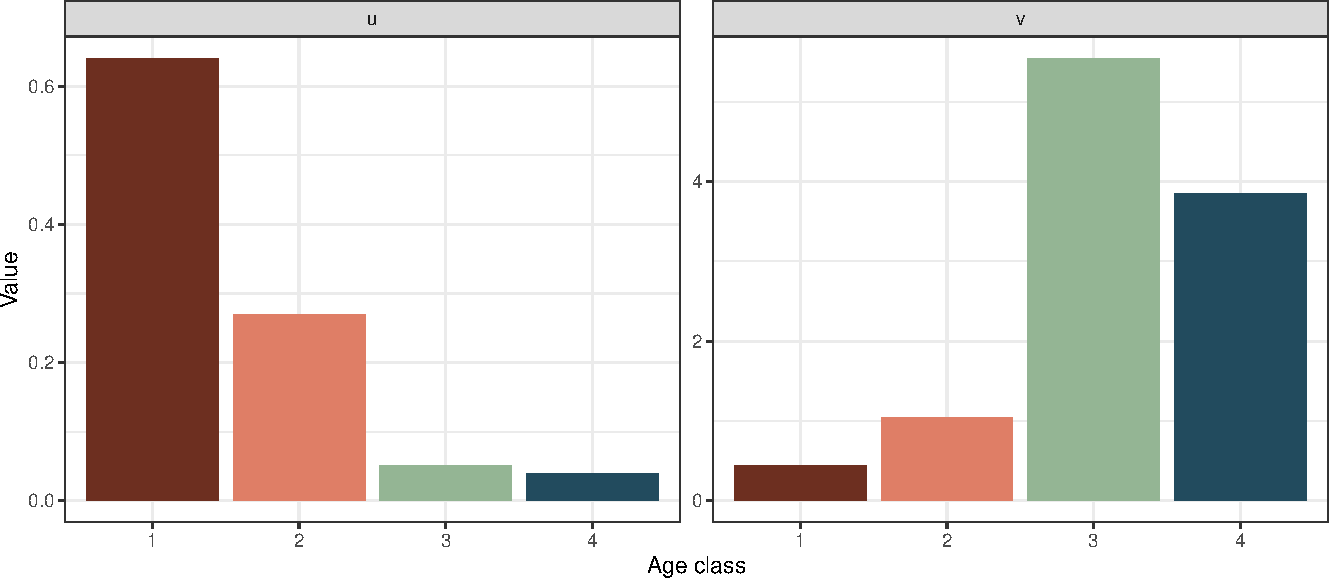
\includegraphics{DemographyCompendium_files/figure-latex/unnamed-chunk-60-1.pdf}

Now that \(\lambda>1\), the stable age structure is declining over age. Compared to before it is also more skewed towards the younger age classes. The reproductive value is still highest in age class 3, but the difference is now larger between the two reproducing classes and the young non-reproducing classes.

\begin{enumerate}
\def\labelenumi{\arabic{enumi}.}
\setcounter{enumi}{7}
\tightlist
\item
  Increase survival by factor \(c\) to get \(\lambda>1\):
\end{enumerate}

Based on trial and error (apply the code several times for different values of c) we find the value of c that increases the survival enough to get lambda \textgreater1 (NB: Note that we need to update both the fertility and survival coefficients):

\begin{Shaded}
\begin{Highlighting}[]
\NormalTok{C }\OtherTok{\textless{}{-}} \FloatTok{1.8} \CommentTok{\#Updated through trial and error }
\NormalTok{AmatPlantNew2 }\OtherTok{\textless{}{-}} \FunctionTok{Create.Amat}\NormalTok{(}\AttributeTok{Svec=}\NormalTok{px[}\DecValTok{2}\SpecialCharTok{:}\DecValTok{5}\NormalTok{] }\SpecialCharTok{*}\NormalTok{C, }\AttributeTok{Fvec=}\NormalTok{px[}\DecValTok{1}\NormalTok{]}\SpecialCharTok{*}\NormalTok{mx[}\DecValTok{2}\SpecialCharTok{:}\DecValTok{5}\NormalTok{]}\SpecialCharTok{*}\NormalTok{C)}
\NormalTok{FmatPlantNew2 }\OtherTok{\textless{}{-}}\NormalTok{ UmatPlantNew2 }\OtherTok{\textless{}{-}}\NormalTok{ AmatPlantNew2}

\NormalTok{FmatPlantNew2[}\SpecialCharTok{{-}}\DecValTok{1}\NormalTok{,] }\OtherTok{\textless{}{-}} \DecValTok{0} \CommentTok{\#Set all elements to zero that are not on the first row}
\NormalTok{UmatPlantNew2[}\DecValTok{1}\NormalTok{,] }\OtherTok{\textless{}{-}} \DecValTok{0} \CommentTok{\#Set all elements to zero in the first row}

\FunctionTok{uvlambda}\NormalTok{(AmatPlantNew2)}\SpecialCharTok{$}\NormalTok{lambda}
\end{Highlighting}
\end{Shaded}

\begin{verbatim}
## [1] 1.016965
\end{verbatim}

With a multiplying factor of 1.8 for the survival vector to get \(\lambda\) over 1, however this means that the survival probability of the third age class is \(>1\), which is not realistic/possible.

\hypertarget{post-reproductive-census-1}{%
\subsubsection*{Post-reproductive census:}\label{post-reproductive-census-1}}
\addcontentsline{toc}{subsubsection}{Post-reproductive census:}

\begin{enumerate}
\def\labelenumi{\arabic{enumi}.}
\tightlist
\item
  Life cycle graph of the plant:
\end{enumerate}

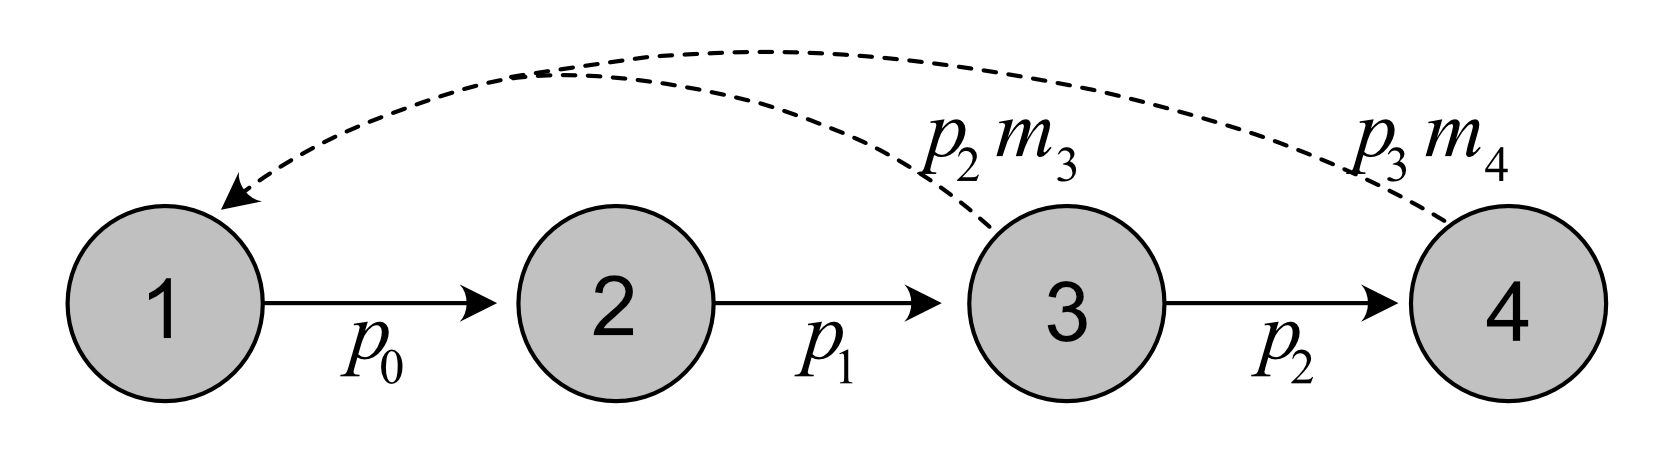
\includegraphics[width=0.6\linewidth]{LifeCyclePlantPost}

\begin{enumerate}
\def\labelenumi{\arabic{enumi}.}
\setcounter{enumi}{1}
\tightlist
\item
  Vectors of fertility and survival coefficients:
\end{enumerate}

\begin{Shaded}
\begin{Highlighting}[]
\NormalTok{fertility.plant.post }\OtherTok{\textless{}{-}}\NormalTok{ px[}\DecValTok{1}\SpecialCharTok{:}\DecValTok{4}\NormalTok{]}\SpecialCharTok{*}\NormalTok{mx[}\DecValTok{2}\SpecialCharTok{:}\DecValTok{5}\NormalTok{] }\CommentTok{\#corresponding to age class 1:4, age 0:3}
\NormalTok{survival.plant.post }\OtherTok{\textless{}{-}} \FunctionTok{c}\NormalTok{(px[}\DecValTok{1}\SpecialCharTok{:}\DecValTok{3}\NormalTok{],}\DecValTok{0}\NormalTok{) }\CommentTok{\#corresponding to age class 1:4, age 0:3}
\end{Highlighting}
\end{Shaded}

\begin{enumerate}
\def\labelenumi{\arabic{enumi}.}
\setcounter{enumi}{2}
\tightlist
\item
  Define \(\mathbf{A}\), \(\mathbf{U}\) and \(\mathbf{F}\):
\end{enumerate}

\begin{Shaded}
\begin{Highlighting}[]
\NormalTok{AmatPlant.post }\OtherTok{\textless{}{-}} \FunctionTok{Create.Amat}\NormalTok{(}\AttributeTok{Svec=}\NormalTok{survival.plant.post, }\AttributeTok{Fvec=}\NormalTok{fertility.plant.post)}
\NormalTok{FmatPlant.post }\OtherTok{\textless{}{-}}\NormalTok{ UmatPlant.post }\OtherTok{\textless{}{-}}\NormalTok{ AmatPlant.post}

\NormalTok{FmatPlant.post[}\SpecialCharTok{{-}}\DecValTok{1}\NormalTok{,] }\OtherTok{\textless{}{-}} \DecValTok{0} \CommentTok{\#Set all elements to zero that are not on the first row}
\NormalTok{UmatPlant.post[}\DecValTok{1}\NormalTok{,] }\OtherTok{\textless{}{-}} \DecValTok{0} \CommentTok{\#Set all elements to zero in the first row}

\NormalTok{AmatPlant.post}
\end{Highlighting}
\end{Shaded}

\begin{verbatim}
##          [,1]      [,2]      [,3]     [,4]
## [1,] 0.000000 0.0000000 0.3988827 2.522353
## [2,] 0.342033 0.0000000 0.0000000 0.000000
## [3,] 0.000000 0.4228679 0.0000000 0.000000
## [4,] 0.000000 0.0000000 0.1899441 0.000000
\end{verbatim}

\begin{enumerate}
\def\labelenumi{\arabic{enumi}.}
\setcounter{enumi}{3}
\tightlist
\item
  Project age classes over 30 time steps:
\end{enumerate}

\begin{Shaded}
\begin{Highlighting}[]
\CommentTok{\#Return matrix of projected growth of each age class over time:}
\NormalTok{Pop.plant.post }\OtherTok{\textless{}{-}} \FunctionTok{projection}\NormalTok{(}\AttributeTok{MatA=}\NormalTok{AmatPlant.post, }\AttributeTok{n0=}\FunctionTok{rep}\NormalTok{(}\DecValTok{10}\NormalTok{, }\DecValTok{4}\NormalTok{), }\AttributeTok{Tmax=}\DecValTok{30}\NormalTok{)}
 
\CommentTok{\#Long format for plotting:}
\NormalTok{Pop.plant.long.post }\OtherTok{\textless{}{-}}\NormalTok{ Pop.plant.post }\SpecialCharTok{\%\textgreater{}\%} \FunctionTok{pivot\_longer}\NormalTok{(}\FunctionTok{c}\NormalTok{(}\SpecialCharTok{{-}}\NormalTok{time),}
               \AttributeTok{names\_to =} \StringTok{"AgeClass"}\NormalTok{, }\AttributeTok{values\_to =} \StringTok{"Value"}\NormalTok{)}

\CommentTok{\#Plot}
\FunctionTok{ggplot}\NormalTok{(Pop.plant.long.post) }\SpecialCharTok{+} 
  \FunctionTok{geom\_line}\NormalTok{(}\FunctionTok{aes}\NormalTok{(}\AttributeTok{x=}\NormalTok{time,}\AttributeTok{y=}\NormalTok{Value, }\AttributeTok{col=}\NormalTok{AgeClass, }\AttributeTok{linetype=}\NormalTok{AgeClass), }\AttributeTok{lwd=}\FloatTok{1.2}\NormalTok{)}\SpecialCharTok{+}
  \FunctionTok{theme\_bw}\NormalTok{() }\SpecialCharTok{+}
  \FunctionTok{scale\_color\_manual}\NormalTok{(}\AttributeTok{values=}\NormalTok{colors4)}\SpecialCharTok{+} \CommentTok{\#Add colors manually}
  \FunctionTok{scale\_linetype\_manual}\NormalTok{(}\AttributeTok{values=}\DecValTok{1}\SpecialCharTok{:}\DecValTok{4}\NormalTok{)}\SpecialCharTok{+} \CommentTok{\#Add linetypes manually}
  \FunctionTok{labs}\NormalTok{( }\AttributeTok{x=}\StringTok{"Time (year)"}\NormalTok{, }\AttributeTok{y=}\StringTok{"Age class size"}\NormalTok{)}\SpecialCharTok{+} \CommentTok{\#Axis labels}
  \FunctionTok{theme}\NormalTok{(}\AttributeTok{legend.position =} \StringTok{"top"}\NormalTok{ ) }\CommentTok{\#Place legend on top}
\end{Highlighting}
\end{Shaded}

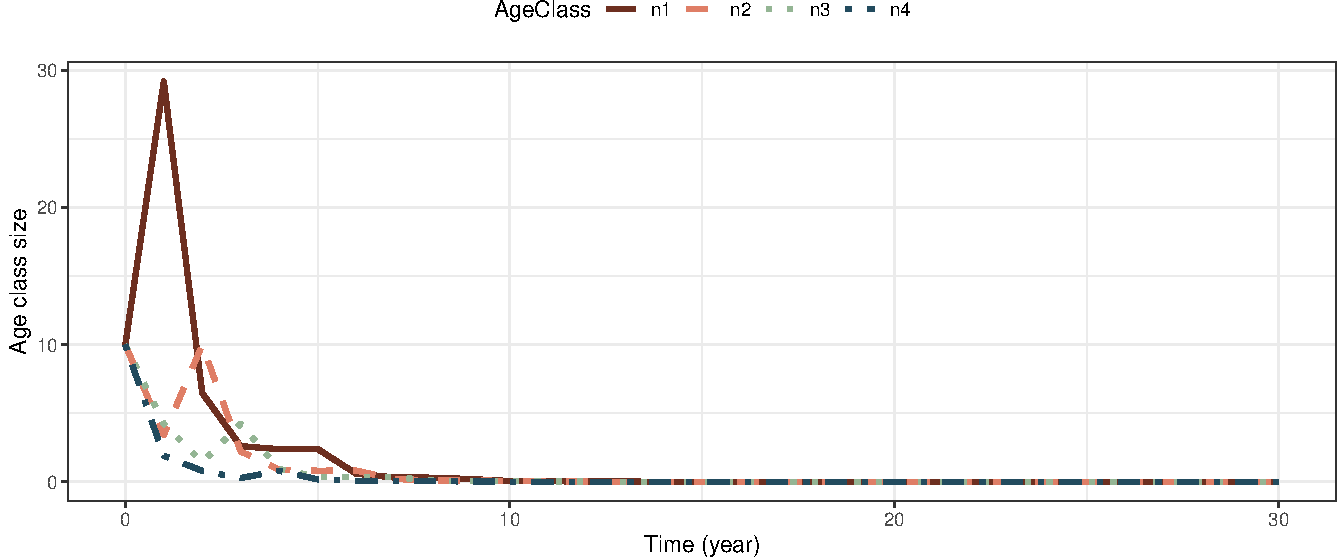
\includegraphics{DemographyCompendium_files/figure-latex/unnamed-chunk-65-1.pdf}

\begin{enumerate}
\def\labelenumi{\arabic{enumi}.}
\setcounter{enumi}{4}
\tightlist
\item
  Calculate \(\lambda\), \(R_0\) and \(G\) using the matrices:
\end{enumerate}

\begin{Shaded}
\begin{Highlighting}[]
\NormalTok{res.plant.post }\OtherTok{\textless{}{-}} \FunctionTok{uvlambda}\NormalTok{(AmatPlant.post)}
\NormalTok{lambda.plant.post }\OtherTok{\textless{}{-}}\NormalTok{ res.plant.post}\SpecialCharTok{$}\NormalTok{lambda}
\NormalTok{R0.plant.post }\OtherTok{\textless{}{-}} \FunctionTok{R0function}\NormalTok{(UmatPlant.post, FmatPlant.post)}\SpecialCharTok{$}\NormalTok{R0}
\NormalTok{G.plant.post }\OtherTok{\textless{}{-}} \FunctionTok{GenTime}\NormalTok{(AmatPlant.post, FmatPlant.post)}

\NormalTok{ResVec.post }\OtherTok{\textless{}{-}} \FunctionTok{c}\NormalTok{(lambda.plant.post, R0.plant.post, G.plant.post) }\CommentTok{\#Store results}
\FunctionTok{names}\NormalTok{(ResVec.post) }\OtherTok{\textless{}{-}} \FunctionTok{c}\NormalTok{(}\StringTok{"lambda"}\NormalTok{, }\StringTok{"R0"}\NormalTok{, }\StringTok{"G"}\NormalTok{)}
\FunctionTok{round}\NormalTok{(ResVec.post,}\DecValTok{3}\NormalTok{)}
\end{Highlighting}
\end{Shaded}

\begin{verbatim}
## lambda     R0      G 
##  0.565  0.127  3.680
\end{verbatim}

The values are the same as with the pre-reproductive census model.

\begin{enumerate}
\def\labelenumi{\arabic{enumi}.}
\setcounter{enumi}{5}
\tightlist
\item
  Calculate and plot \(\mathbf{u}\) and \(\mathbf{v}\):
\end{enumerate}

These values were calculated in the previous point using the R function \texttt{uvlambda()}. To plot them:

\begin{Shaded}
\begin{Highlighting}[]
\CommentTok{\#Create data frame for plotting}
\NormalTok{plantframe.post }\OtherTok{\textless{}{-}} \FunctionTok{data.frame}\NormalTok{(}\StringTok{"AgeClass"}\OtherTok{=}\FunctionTok{factor}\NormalTok{(}\DecValTok{1}\SpecialCharTok{:}\DecValTok{4}\NormalTok{), }\StringTok{"u"}\OtherTok{=}\NormalTok{res.plant.post}\SpecialCharTok{$}\NormalTok{u, }\StringTok{"v"}\OtherTok{=}\FunctionTok{t}\NormalTok{(res.plant.post}\SpecialCharTok{$}\NormalTok{v))}

\CommentTok{\#Long format for plotting:}
\NormalTok{plantframe.post.long }\OtherTok{\textless{}{-}}\NormalTok{ plantframe.post }\SpecialCharTok{\%\textgreater{}\%} \FunctionTok{pivot\_longer}\NormalTok{(}\FunctionTok{c}\NormalTok{(u,v),}
               \AttributeTok{names\_to =} \StringTok{"Vector"}\NormalTok{, }\AttributeTok{values\_to =} \StringTok{"Value"}\NormalTok{)}

 
\CommentTok{\#Plot}
\FunctionTok{ggplot}\NormalTok{(plantframe.post.long) }\SpecialCharTok{+} 
  \FunctionTok{geom\_col}\NormalTok{(}\FunctionTok{aes}\NormalTok{(}\AttributeTok{x=}\NormalTok{AgeClass, }\AttributeTok{y=}\NormalTok{Value, }\AttributeTok{fill=}\NormalTok{AgeClass ), }\AttributeTok{lwd=}\FloatTok{1.2}\NormalTok{)}\SpecialCharTok{+}
  \FunctionTok{theme\_bw}\NormalTok{() }\SpecialCharTok{+}
  \FunctionTok{facet\_wrap}\NormalTok{(}\FunctionTok{vars}\NormalTok{(Vector),}\AttributeTok{ncol=}\DecValTok{2}\NormalTok{,}\AttributeTok{scales=}\StringTok{"free"}\NormalTok{)}\SpecialCharTok{+}
  \FunctionTok{scale\_fill\_manual}\NormalTok{(}\AttributeTok{values=}\NormalTok{colors4)}\SpecialCharTok{+} \CommentTok{\#Add colors manually}
  \FunctionTok{labs}\NormalTok{( }\AttributeTok{x=}\StringTok{"Age class"}\NormalTok{, }\AttributeTok{y=}\StringTok{"Value"}\NormalTok{)}\SpecialCharTok{+} \CommentTok{\#Axis labels}
  \FunctionTok{theme}\NormalTok{(}\AttributeTok{legend.position =} \StringTok{"none"}\NormalTok{ ) }\CommentTok{\#Drop legend}
\end{Highlighting}
\end{Shaded}

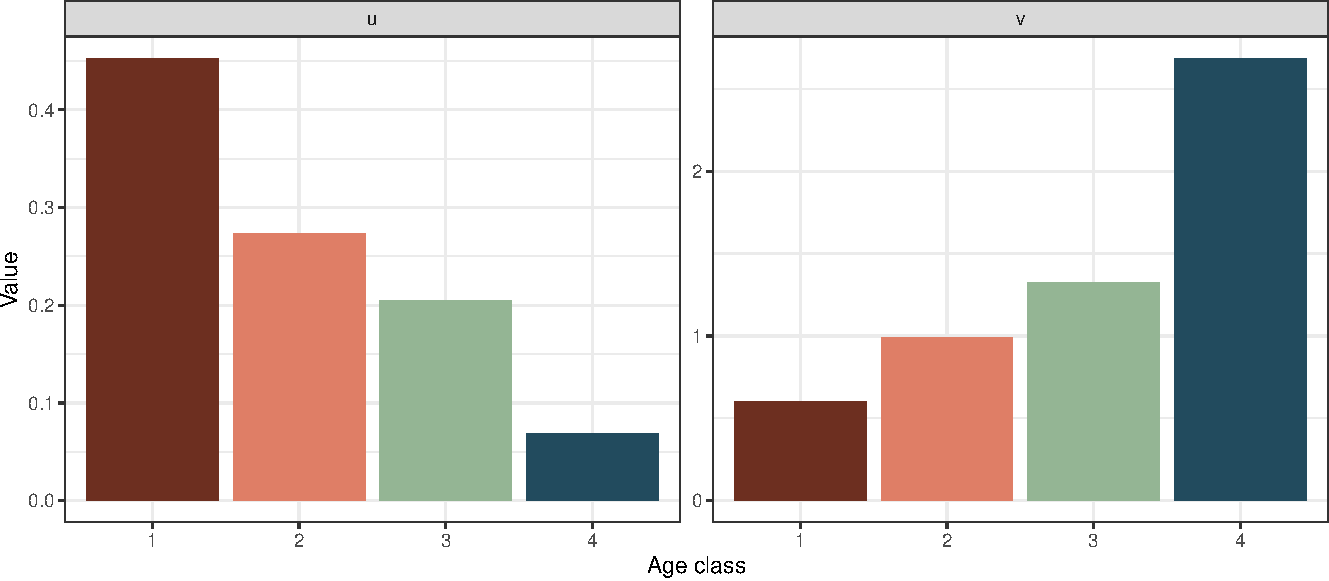
\includegraphics{DemographyCompendium_files/figure-latex/unnamed-chunk-67-1.pdf}

Now the age classes correspond to actual age 0 to 3, in contrast to the pre-reproductive model where they correspond to age 1 to 4. The stable age structure and reproductive values look different here, since the classes represent other ages. Here the highest reproductive value is found for age class 4, corresponding to age 3. This is in line with the result from the pre-reproductive model where the highest reproductive value was found in age class 3, there corresponding to age 3.

\begin{enumerate}
\def\labelenumi{\arabic{enumi}.}
\setcounter{enumi}{6}
\tightlist
\item
  Increase fecundity by factor \(c\) to get \(\lambda>1\):
\end{enumerate}

Based on trial and error (apply the code several times for different values of c) we find the value of c that increases the fecundity enough to get lambda \textgreater1:

\begin{Shaded}
\begin{Highlighting}[]
\NormalTok{C }\OtherTok{\textless{}{-}} \DecValTok{8} \CommentTok{\#Updated through trial and error }
\NormalTok{AmatPlantNew.post }\OtherTok{\textless{}{-}} \FunctionTok{Create.Amat}\NormalTok{(}\AttributeTok{Svec=} \FunctionTok{c}\NormalTok{(px[}\DecValTok{1}\SpecialCharTok{:}\DecValTok{3}\NormalTok{],}\DecValTok{0}\NormalTok{), }\AttributeTok{Fvec=}\NormalTok{px[}\DecValTok{1}\SpecialCharTok{:}\DecValTok{4}\NormalTok{]}\SpecialCharTok{*}\NormalTok{mx[}\DecValTok{2}\SpecialCharTok{:}\DecValTok{5}\NormalTok{]}\SpecialCharTok{*}\NormalTok{C)}
\NormalTok{FmatPlantNew.post }\OtherTok{\textless{}{-}}\NormalTok{ UmatPlantNew.post }\OtherTok{\textless{}{-}}\NormalTok{ AmatPlantNew.post}

\NormalTok{FmatPlantNew.post[}\SpecialCharTok{{-}}\DecValTok{1}\NormalTok{,] }\OtherTok{\textless{}{-}} \DecValTok{0} \CommentTok{\#Set all elements to zero that are not on the first row}
\NormalTok{UmatPlantNew.post[}\DecValTok{1}\NormalTok{,] }\OtherTok{\textless{}{-}} \DecValTok{0} \CommentTok{\#Set all elements to zero in the first row}

\FunctionTok{uvlambda}\NormalTok{(AmatPlantNew.post)}\SpecialCharTok{$}\NormalTok{lambda}
\end{Highlighting}
\end{Shaded}

\begin{verbatim}
## [1] 1.00446
\end{verbatim}

We need the same factor of 8 (increasing fecundity 8 times) to get \(\lambda\) over 1.

The other parameters

\begin{Shaded}
\begin{Highlighting}[]
\NormalTok{res.plantNew.post }\OtherTok{\textless{}{-}} \FunctionTok{uvlambda}\NormalTok{(AmatPlantNew.post)}
\NormalTok{lambda.plantNew.post }\OtherTok{\textless{}{-}}\NormalTok{ res.plantNew.post}\SpecialCharTok{$}\NormalTok{lambda}
\NormalTok{R0.plantNew.post }\OtherTok{\textless{}{-}} \FunctionTok{R0function}\NormalTok{(UmatPlantNew.post, FmatPlantNew.post)}\SpecialCharTok{$}\NormalTok{R0}
\NormalTok{G.plantNew.post }\OtherTok{\textless{}{-}} \FunctionTok{GenTime}\NormalTok{(AmatPlantNew.post, FmatPlantNew.post)}

\NormalTok{ResVecNew.post }\OtherTok{\textless{}{-}} \FunctionTok{c}\NormalTok{(lambda.plantNew.post, R0.plantNew.post, G.plantNew.post) }\CommentTok{\#Store results}
\FunctionTok{names}\NormalTok{(ResVecNew.post) }\OtherTok{\textless{}{-}} \FunctionTok{c}\NormalTok{(}\StringTok{"lambda"}\NormalTok{, }\StringTok{"R0"}\NormalTok{, }\StringTok{"G"}\NormalTok{)}
\FunctionTok{round}\NormalTok{(ResVecNew.post,}\DecValTok{3}\NormalTok{)}
\end{Highlighting}
\end{Shaded}

\begin{verbatim}
## lambda     R0      G 
##  1.004  1.016  3.545
\end{verbatim}

These values are the same as in the pre-reproductive (updated) model.

Plot new stable structure and reproductive values

\begin{Shaded}
\begin{Highlighting}[]
\CommentTok{\#Create data frame for plotting}
\NormalTok{plantframeNew.post }\OtherTok{\textless{}{-}} \FunctionTok{data.frame}\NormalTok{(}\StringTok{"AgeClass"}\OtherTok{=}\FunctionTok{factor}\NormalTok{(}\DecValTok{1}\SpecialCharTok{:}\DecValTok{4}\NormalTok{), }\StringTok{"u"}\OtherTok{=}\NormalTok{res.plantNew.post}\SpecialCharTok{$}\NormalTok{u, }\StringTok{"v"}\OtherTok{=}\FunctionTok{t}\NormalTok{(res.plantNew.post}\SpecialCharTok{$}\NormalTok{v))}

\CommentTok{\#Long format for plotting:}
\NormalTok{plantframeNew.post.long }\OtherTok{\textless{}{-}}\NormalTok{ plantframeNew.post }\SpecialCharTok{\%\textgreater{}\%} \FunctionTok{pivot\_longer}\NormalTok{(}\FunctionTok{c}\NormalTok{(u,v),}
               \AttributeTok{names\_to =} \StringTok{"Vector"}\NormalTok{, }\AttributeTok{values\_to =} \StringTok{"Value"}\NormalTok{)}

 
\CommentTok{\#Plot}
\FunctionTok{ggplot}\NormalTok{(plantframeNew.post.long) }\SpecialCharTok{+} 
  \FunctionTok{geom\_col}\NormalTok{(}\FunctionTok{aes}\NormalTok{(}\AttributeTok{x=}\NormalTok{AgeClass, }\AttributeTok{y=}\NormalTok{Value, }\AttributeTok{fill=}\NormalTok{AgeClass ), }\AttributeTok{lwd=}\FloatTok{1.2}\NormalTok{)}\SpecialCharTok{+}
  \FunctionTok{theme\_bw}\NormalTok{() }\SpecialCharTok{+}
  \FunctionTok{facet\_wrap}\NormalTok{(}\FunctionTok{vars}\NormalTok{(Vector),}\AttributeTok{ncol=}\DecValTok{2}\NormalTok{,}\AttributeTok{scales=}\StringTok{"free"}\NormalTok{)}\SpecialCharTok{+}
  \FunctionTok{scale\_fill\_manual}\NormalTok{(}\AttributeTok{values=}\NormalTok{colors4)}\SpecialCharTok{+} \CommentTok{\#Add colors manually}
  \FunctionTok{labs}\NormalTok{( }\AttributeTok{x=}\StringTok{"Age class"}\NormalTok{, }\AttributeTok{y=}\StringTok{"Value"}\NormalTok{)}\SpecialCharTok{+} \CommentTok{\#Axis labels}
  \FunctionTok{theme}\NormalTok{(}\AttributeTok{legend.position =} \StringTok{"none"}\NormalTok{ ) }\CommentTok{\#Drop legend}
\end{Highlighting}
\end{Shaded}

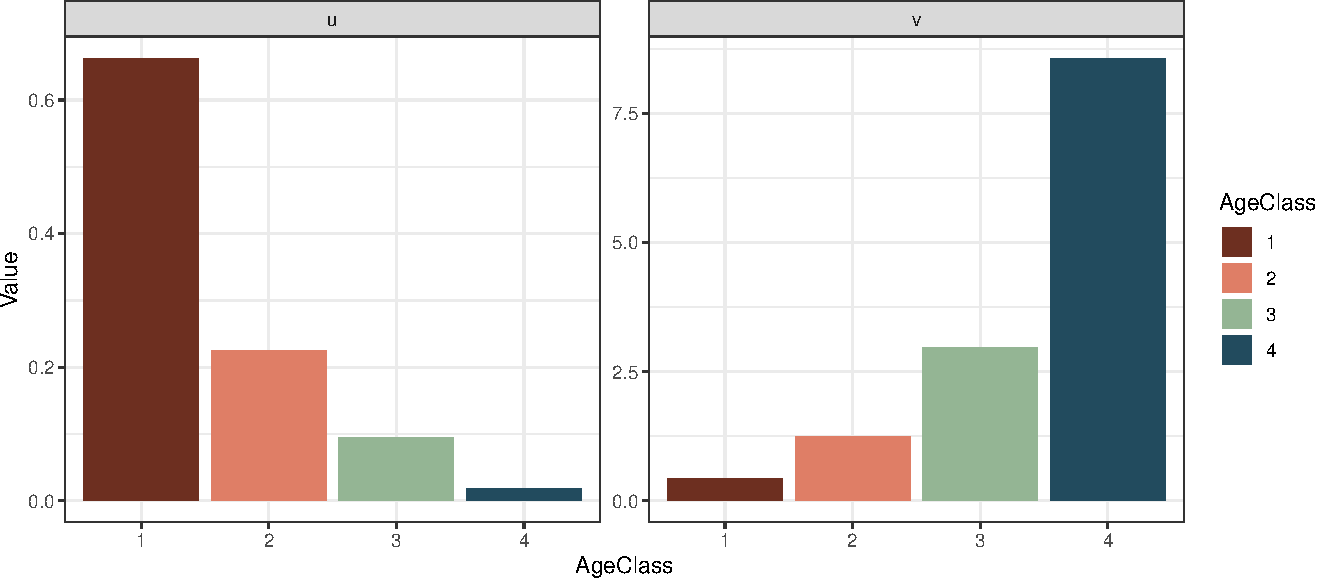
\includegraphics{DemographyCompendium_files/figure-latex/unnamed-chunk-70-1.pdf}

Compared to before, the stable structure is more skewed towards the younger age classes. The reproductive value is still highest in age class 4, but the difference is now larger between the classes.

\begin{enumerate}
\def\labelenumi{\arabic{enumi}.}
\setcounter{enumi}{7}
\tightlist
\item
  Increase survival by factor \(c\) to get \(\lambda>1\):
\end{enumerate}

Based on trial and error (apply the code several times for different values of c) we find the value of c that increases the fecundity enough to get lambda \textgreater1:

\begin{Shaded}
\begin{Highlighting}[]
\NormalTok{C }\OtherTok{\textless{}{-}} \FloatTok{1.8} \CommentTok{\#Updated through trial and error }
\NormalTok{AmatPlantNew2.post }\OtherTok{\textless{}{-}} \FunctionTok{Create.Amat}\NormalTok{(}\AttributeTok{Svec=} \FunctionTok{c}\NormalTok{(px[}\DecValTok{1}\SpecialCharTok{:}\DecValTok{3}\NormalTok{],}\DecValTok{0}\NormalTok{)}\SpecialCharTok{*}\NormalTok{C, }\AttributeTok{Fvec=}\NormalTok{px[}\DecValTok{1}\SpecialCharTok{:}\DecValTok{4}\NormalTok{]}\SpecialCharTok{*}\NormalTok{mx[}\DecValTok{2}\SpecialCharTok{:}\DecValTok{5}\NormalTok{]}\SpecialCharTok{*}\NormalTok{C)}
\NormalTok{FmatPlantNew2.post }\OtherTok{\textless{}{-}}\NormalTok{ UmatPlantNew2.post }\OtherTok{\textless{}{-}}\NormalTok{ AmatPlantNew2.post}

\NormalTok{FmatPlantNew2.post[}\SpecialCharTok{{-}}\DecValTok{1}\NormalTok{,] }\OtherTok{\textless{}{-}} \DecValTok{0} \CommentTok{\#Set all elements to zero that are not on the first row}
\NormalTok{UmatPlantNew2.post[}\DecValTok{1}\NormalTok{,] }\OtherTok{\textless{}{-}} \DecValTok{0} \CommentTok{\#Set all elements to zero in the first row}

\FunctionTok{uvlambda}\NormalTok{(AmatPlantNew2.post)}\SpecialCharTok{$}\NormalTok{lambda}
\end{Highlighting}
\end{Shaded}

\begin{verbatim}
## [1] 1.016965
\end{verbatim}

We still need a multiplying factor of 1.8 for survival to get \(\lambda\) over 1, and we get the same problem with \(p_3>1\).

\hypertarget{chapter-4-exercises}{%
\section{Chapter 4 exercises}\label{chapter-4-exercises}}

\hypertarget{exercise-4.1-1}{%
\subsection*{Exercise 4.1}\label{exercise-4.1-1}}
\addcontentsline{toc}{subsection}{Exercise 4.1}

\begin{enumerate}
\def\labelenumi{\arabic{enumi}.}
\item
\end{enumerate}

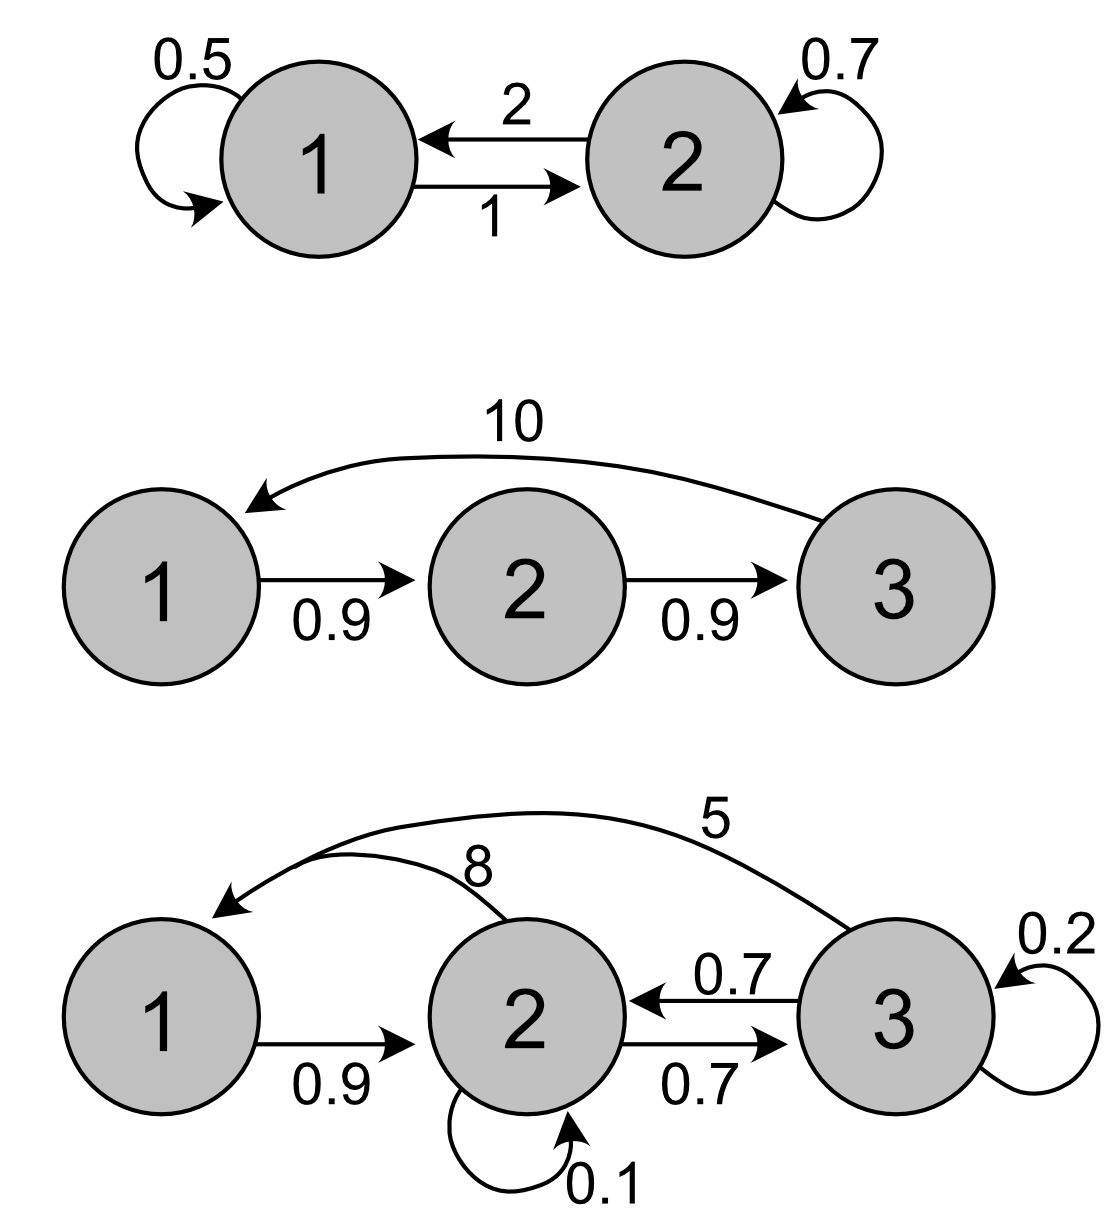
\includegraphics[width=0.6\linewidth]{LifeCycleEx41}

\begin{enumerate}
\def\labelenumi{\arabic{enumi}.}
\setcounter{enumi}{1}
\tightlist
\item
  To separate out the vectors of survival probabilities and fertility coefficients, we need the matrices \(\mathbf{U}\) and \(\mathbf{F}\), instead of only \(\mathbf{A}\). If we assume that the first row of \(\mathbf{A}\) represent fertilities and the others represent survival and transitions, we can decompose \(\mathbf{A}\) (note that in general this is not an assumption we can make):
\end{enumerate}

\begin{Shaded}
\begin{Highlighting}[]
\CommentTok{\# Create the projection matrices in R:}
\NormalTok{Amat1 }\OtherTok{\textless{}{-}} \FunctionTok{cbind}\NormalTok{(}\FunctionTok{c}\NormalTok{(.}\DecValTok{5}\NormalTok{, }\DecValTok{1}\NormalTok{), }\FunctionTok{c}\NormalTok{(}\DecValTok{2}\NormalTok{,.}\DecValTok{7}\NormalTok{))}
\NormalTok{Amat2 }\OtherTok{\textless{}{-}} \FunctionTok{cbind}\NormalTok{(}\FunctionTok{c}\NormalTok{(}\DecValTok{0}\NormalTok{, .}\DecValTok{9}\NormalTok{, }\DecValTok{0}\NormalTok{), }\FunctionTok{c}\NormalTok{(}\DecValTok{0}\NormalTok{, }\DecValTok{0}\NormalTok{, .}\DecValTok{9}\NormalTok{), }\FunctionTok{c}\NormalTok{(}\DecValTok{10}\NormalTok{, }\DecValTok{0}\NormalTok{, }\DecValTok{0}\NormalTok{))}
\NormalTok{Amat3 }\OtherTok{\textless{}{-}} \FunctionTok{cbind}\NormalTok{(}\FunctionTok{c}\NormalTok{(}\DecValTok{0}\NormalTok{, .}\DecValTok{9}\NormalTok{, }\DecValTok{0}\NormalTok{), }\FunctionTok{c}\NormalTok{(}\DecValTok{8}\NormalTok{, .}\DecValTok{1}\NormalTok{, .}\DecValTok{7}\NormalTok{), }\FunctionTok{c}\NormalTok{(}\DecValTok{5}\NormalTok{, .}\DecValTok{7}\NormalTok{, .}\DecValTok{2}\NormalTok{))}

\CommentTok{\# Create matrices U and F for each example, under the assumption mentioned:}
\NormalTok{Umat1 }\OtherTok{\textless{}{-}} \FunctionTok{cbind}\NormalTok{(}\FunctionTok{c}\NormalTok{(}\DecValTok{0}\NormalTok{, }\DecValTok{1}\NormalTok{), }\FunctionTok{c}\NormalTok{(}\DecValTok{0}\NormalTok{,.}\DecValTok{7}\NormalTok{))}
\NormalTok{Umat2 }\OtherTok{\textless{}{-}} \FunctionTok{cbind}\NormalTok{(}\FunctionTok{c}\NormalTok{(}\DecValTok{0}\NormalTok{, .}\DecValTok{9}\NormalTok{, }\DecValTok{0}\NormalTok{), }\FunctionTok{c}\NormalTok{(}\DecValTok{0}\NormalTok{, }\DecValTok{0}\NormalTok{, .}\DecValTok{9}\NormalTok{), }\FunctionTok{c}\NormalTok{(}\DecValTok{0}\NormalTok{, }\DecValTok{0}\NormalTok{, }\DecValTok{0}\NormalTok{))}
\NormalTok{Umat3 }\OtherTok{\textless{}{-}} \FunctionTok{cbind}\NormalTok{(}\FunctionTok{c}\NormalTok{(}\DecValTok{0}\NormalTok{, .}\DecValTok{9}\NormalTok{, }\DecValTok{0}\NormalTok{), }\FunctionTok{c}\NormalTok{(}\DecValTok{0}\NormalTok{, .}\DecValTok{1}\NormalTok{, .}\DecValTok{7}\NormalTok{), }\FunctionTok{c}\NormalTok{(}\DecValTok{0}\NormalTok{, .}\DecValTok{7}\NormalTok{, .}\DecValTok{2}\NormalTok{))}

\NormalTok{Fmat1 }\OtherTok{\textless{}{-}} \FunctionTok{cbind}\NormalTok{(}\FunctionTok{c}\NormalTok{(.}\DecValTok{5}\NormalTok{, }\DecValTok{0}\NormalTok{), }\FunctionTok{c}\NormalTok{(}\DecValTok{2}\NormalTok{, }\DecValTok{0}\NormalTok{))}
\NormalTok{Fmat2 }\OtherTok{\textless{}{-}} \FunctionTok{cbind}\NormalTok{(}\FunctionTok{c}\NormalTok{(}\DecValTok{0}\NormalTok{, }\DecValTok{0}\NormalTok{, }\DecValTok{0}\NormalTok{), }\FunctionTok{c}\NormalTok{(}\DecValTok{0}\NormalTok{, }\DecValTok{0}\NormalTok{, }\DecValTok{0}\NormalTok{), }\FunctionTok{c}\NormalTok{(}\DecValTok{10}\NormalTok{, }\DecValTok{0}\NormalTok{, }\DecValTok{0}\NormalTok{))}
\NormalTok{Fmat3 }\OtherTok{\textless{}{-}} \FunctionTok{cbind}\NormalTok{(}\FunctionTok{c}\NormalTok{(}\DecValTok{0}\NormalTok{, }\DecValTok{0}\NormalTok{, }\DecValTok{0}\NormalTok{), }\FunctionTok{c}\NormalTok{(}\DecValTok{8}\NormalTok{, }\DecValTok{0}\NormalTok{, }\DecValTok{0}\NormalTok{), }\FunctionTok{c}\NormalTok{(}\DecValTok{5}\NormalTok{, }\DecValTok{0}\NormalTok{, }\DecValTok{0}\NormalTok{))}

\CommentTok{\#Apply the decompose functions to decompose each matrix (shown here for the first only)}

\FunctionTok{DecomposeU}\NormalTok{(Umat1)}
\end{Highlighting}
\end{Shaded}

\begin{verbatim}
## $Gmat
##      [,1] [,2]
## [1,]    0    0
## [2,]    1    1
## 
## $Survival
## [1] 1.0 0.7
\end{verbatim}

\begin{Shaded}
\begin{Highlighting}[]
\FunctionTok{DecomposeF}\NormalTok{(Fmat1)}
\end{Highlighting}
\end{Shaded}

\begin{verbatim}
## $Qmat
##      [,1] [,2]
## [1,]    1    1
## [2,]    0    0
## 
## $Fertility
## [1] 0.5 2.0
\end{verbatim}

\begin{enumerate}
\def\labelenumi{\arabic{enumi}.}
\setcounter{enumi}{2}
\tightlist
\item
\end{enumerate}

The first matrix has only two stages, and the numbers suggest reproduction occurs in both, as well as transition of individuals. This could be a model for two habitats with migration between them.

The middle matrix is a typical Leslie matrix. Note that only the last age class reproduces, so this is a semelparous life history.

The third matrix has many transitions, but based on the numbers the first stage seems to be an offspring stage. The two other stages both reproduce, and there are transitions between them. They could represent two habitats, or two size classes (where both growing and shrinking is possible).

\hypertarget{exercise-4.2-1}{%
\subsection*{Exercise 4.2}\label{exercise-4.2-1}}
\addcontentsline{toc}{subsection}{Exercise 4.2}

\begin{enumerate}
\def\labelenumi{\arabic{enumi}.}
\tightlist
\item
  Define the fertility matrix \(\mathbf{F}\), the survival matrix \(\mathbf{U}\), and the projection matrix \(\mathbf{A}\):
\end{enumerate}

\begin{Shaded}
\begin{Highlighting}[]
\CommentTok{\#Define vectors}
\NormalTok{Pvec}\OtherTok{\textless{}{-}} \FunctionTok{c}\NormalTok{(}\FloatTok{0.158}\NormalTok{, }\FloatTok{0.545}\NormalTok{, }\FloatTok{0.539}\NormalTok{, }\FloatTok{0.162}\NormalTok{, }\FloatTok{0.008}\NormalTok{, }\FloatTok{0.136}\NormalTok{, }\FloatTok{0.8}\NormalTok{)}
\NormalTok{Gvec }\OtherTok{\textless{}{-}} \FunctionTok{c}\NormalTok{(}\FloatTok{0.722}\NormalTok{,}\FloatTok{0.244}\NormalTok{, }\FloatTok{0.231}\NormalTok{, }\FloatTok{0.788}\NormalTok{ , }\FloatTok{0.792}\NormalTok{, }\FloatTok{0.664}\NormalTok{,}\DecValTok{0}\NormalTok{)}
\NormalTok{Fvec }\OtherTok{\textless{}{-}} \FunctionTok{c}\NormalTok{(}\DecValTok{0}\NormalTok{, }\DecValTok{0}\NormalTok{, }\DecValTok{0}\NormalTok{, }\FloatTok{2.355}\NormalTok{, }\DecValTok{0}\NormalTok{, }\FloatTok{5.568}\NormalTok{, }\DecValTok{0}\NormalTok{)}

\CommentTok{\#Create matrices:}
\NormalTok{Umat.isopod }\OtherTok{\textless{}{-}}\NormalTok{ Fmat.isopod }\OtherTok{\textless{}{-}} \FunctionTok{matrix}\NormalTok{(}\DecValTok{0}\NormalTok{,}\DecValTok{7}\NormalTok{,}\DecValTok{7}\NormalTok{)}
\NormalTok{Umat.isopod[}\FunctionTok{row}\NormalTok{(Umat.isopod) }\SpecialCharTok{==} \FunctionTok{col}\NormalTok{(Umat.isopod) }\SpecialCharTok{+} \DecValTok{1}\NormalTok{] }\OtherTok{\textless{}{-}}\NormalTok{ Gvec[}\DecValTok{1}\SpecialCharTok{:}\DecValTok{6}\NormalTok{]}
\NormalTok{Umat.isopod[}\FunctionTok{row}\NormalTok{(Umat.isopod) }\SpecialCharTok{==} \FunctionTok{col}\NormalTok{(Umat.isopod)] }\OtherTok{\textless{}{-}}\NormalTok{ Pvec}

\NormalTok{Fmat.isopod[}\DecValTok{1}\NormalTok{,] }\OtherTok{\textless{}{-}}\NormalTok{ Fvec}
\NormalTok{Amat.isopod }\OtherTok{\textless{}{-}}\NormalTok{ Umat.isopod }\SpecialCharTok{+}\NormalTok{ Fmat.isopod}
\end{Highlighting}
\end{Shaded}

\begin{enumerate}
\def\labelenumi{\arabic{enumi}.}
\setcounter{enumi}{1}
\tightlist
\item
  Decompose the matrices \(\mathbf{U}\) and \(\mathbf{F}\), plot the stage-specific fertility and survival probability:
\end{enumerate}

\begin{Shaded}
\begin{Highlighting}[]
\NormalTok{Svec.isopod }\OtherTok{\textless{}{-}} \FunctionTok{DecomposeU}\NormalTok{(Umat.isopod)}\SpecialCharTok{$}\NormalTok{Survival}
\NormalTok{Fvec.isopod }\OtherTok{\textless{}{-}} \FunctionTok{DecomposeF}\NormalTok{(Fmat.isopod)}\SpecialCharTok{$}\NormalTok{Fertility}

\CommentTok{\#Make a data frame for plotting:}
\NormalTok{frame.isopod }\OtherTok{\textless{}{-}} \FunctionTok{data.frame}\NormalTok{(}\StringTok{"Stage"}\OtherTok{=}\FunctionTok{as.factor}\NormalTok{(}\DecValTok{1}\SpecialCharTok{:}\DecValTok{7}\NormalTok{), }\StringTok{"Survival"}\OtherTok{=}\NormalTok{Svec.isopod, }\StringTok{"Fertility"}\OtherTok{=}\NormalTok{Fvec.isopod)}

\CommentTok{\#Long format:}
\NormalTok{frame.isopod.long }\OtherTok{\textless{}{-}}\NormalTok{ frame.isopod }\SpecialCharTok{\%\textgreater{}\%} \FunctionTok{pivot\_longer}\NormalTok{(}\FunctionTok{c}\NormalTok{(Survival, Fertility), }\AttributeTok{names\_to =} \StringTok{"VitalRates"}\NormalTok{, }\AttributeTok{values\_to =} \StringTok{"Value"}\NormalTok{)}
 

\CommentTok{\#Plot with ggplot:}
\FunctionTok{ggplot}\NormalTok{(frame.isopod.long) }\SpecialCharTok{+} 
  \FunctionTok{geom\_col}\NormalTok{(}\FunctionTok{aes}\NormalTok{(}\AttributeTok{x=}\NormalTok{Stage, }\AttributeTok{y=}\NormalTok{Value, }\AttributeTok{fill=}\NormalTok{VitalRates ))}\SpecialCharTok{+}
  \FunctionTok{scale\_fill\_manual}\NormalTok{(}\AttributeTok{values=}\NormalTok{colors2)}\SpecialCharTok{+}
  \FunctionTok{facet\_wrap}\NormalTok{(}\SpecialCharTok{\textasciitilde{}}\FunctionTok{factor}\NormalTok{(VitalRates, }\AttributeTok{levels=}\FunctionTok{c}\NormalTok{(}\StringTok{"Survival"}\NormalTok{, }\StringTok{"Fertility"}\NormalTok{)), }\AttributeTok{scales=}\StringTok{"free"}\NormalTok{)}\SpecialCharTok{+}
  \FunctionTok{theme\_bw}\NormalTok{() }\SpecialCharTok{+}
  \FunctionTok{labs}\NormalTok{( }\AttributeTok{x=}\StringTok{"Stage"}\NormalTok{, }\AttributeTok{y=}\StringTok{"Value"}\NormalTok{)}\SpecialCharTok{+}
  \FunctionTok{theme}\NormalTok{(}\AttributeTok{legend.position =} \StringTok{"none"}\NormalTok{ ) }
\end{Highlighting}
\end{Shaded}

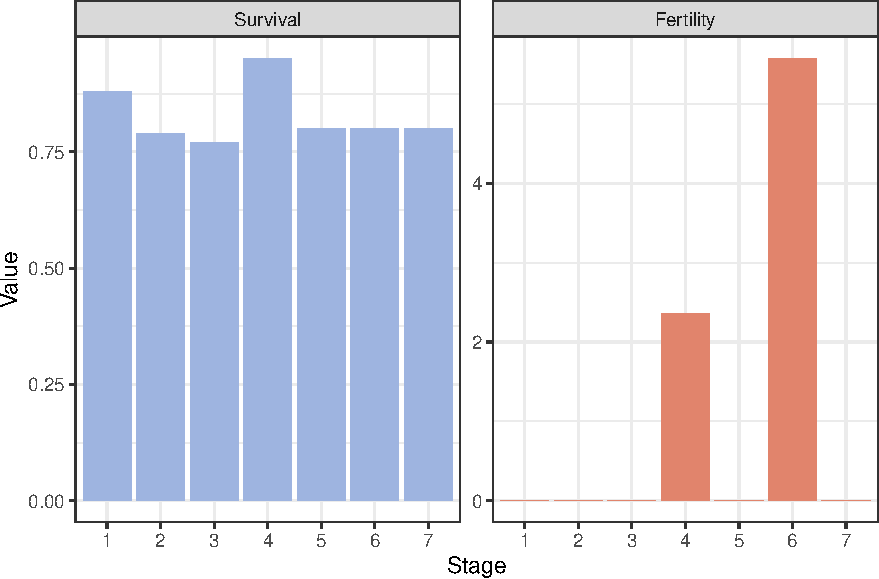
\includegraphics{DemographyCompendium_files/figure-latex/unnamed-chunk-75-1.pdf}

\begin{enumerate}
\def\labelenumi{\arabic{enumi}.}
\setcounter{enumi}{2}
\tightlist
\item
  Calculate \(\lambda\), the stable stage structure and reproductive values, and plot the result:
\end{enumerate}

\begin{Shaded}
\begin{Highlighting}[]
\NormalTok{res.isopod }\OtherTok{\textless{}{-}} \FunctionTok{uvlambda}\NormalTok{(Amat.isopod)}

\NormalTok{lambda.isopod }\OtherTok{\textless{}{-}}\NormalTok{ res.isopod}\SpecialCharTok{$}\NormalTok{lam}

\CommentTok{\#Make a data frame for plotting:}
\NormalTok{resframe.isopod }\OtherTok{\textless{}{-}} \FunctionTok{data.frame}\NormalTok{(}\StringTok{"Stage"}\OtherTok{=}\FunctionTok{as.factor}\NormalTok{(}\DecValTok{1}\SpecialCharTok{:}\DecValTok{7}\NormalTok{), }\StringTok{"u"}\OtherTok{=}\NormalTok{res.isopod}\SpecialCharTok{$}\NormalTok{u, }\StringTok{"v"}\OtherTok{=}\FunctionTok{as.vector}\NormalTok{(res.isopod}\SpecialCharTok{$}\NormalTok{v))}

\CommentTok{\#Long format:}
\NormalTok{resframe.isopod.long }\OtherTok{\textless{}{-}}\NormalTok{ resframe.isopod }\SpecialCharTok{\%\textgreater{}\%} \FunctionTok{pivot\_longer}\NormalTok{(}\FunctionTok{c}\NormalTok{(u, v), }\AttributeTok{names\_to =} \StringTok{"uv"}\NormalTok{, }\AttributeTok{values\_to =} \StringTok{"Value"}\NormalTok{)}
 

\CommentTok{\#Plot with ggplot:}
\FunctionTok{ggplot}\NormalTok{(resframe.isopod.long) }\SpecialCharTok{+} 
  \FunctionTok{geom\_col}\NormalTok{(}\FunctionTok{aes}\NormalTok{(}\AttributeTok{x=}\NormalTok{Stage, }\AttributeTok{y=}\NormalTok{Value, }\AttributeTok{fill=}\NormalTok{uv ))}\SpecialCharTok{+}
  \FunctionTok{scale\_fill\_manual}\NormalTok{(}\AttributeTok{values=}\NormalTok{colors2)}\SpecialCharTok{+}
  \FunctionTok{facet\_wrap}\NormalTok{(}\SpecialCharTok{\textasciitilde{}}\FunctionTok{factor}\NormalTok{(uv, }\AttributeTok{levels=}\FunctionTok{c}\NormalTok{(}\StringTok{"u"}\NormalTok{, }\StringTok{"v"}\NormalTok{)), }\AttributeTok{scales=}\StringTok{"free"}\NormalTok{)}\SpecialCharTok{+}
  \FunctionTok{theme\_bw}\NormalTok{() }\SpecialCharTok{+}
  \FunctionTok{labs}\NormalTok{( }\AttributeTok{x=}\StringTok{"Stage"}\NormalTok{, }\AttributeTok{y=}\StringTok{"Value"}\NormalTok{)}\SpecialCharTok{+}
  \FunctionTok{theme}\NormalTok{(}\AttributeTok{legend.position =} \StringTok{"none"}\NormalTok{ ) }
\end{Highlighting}
\end{Shaded}

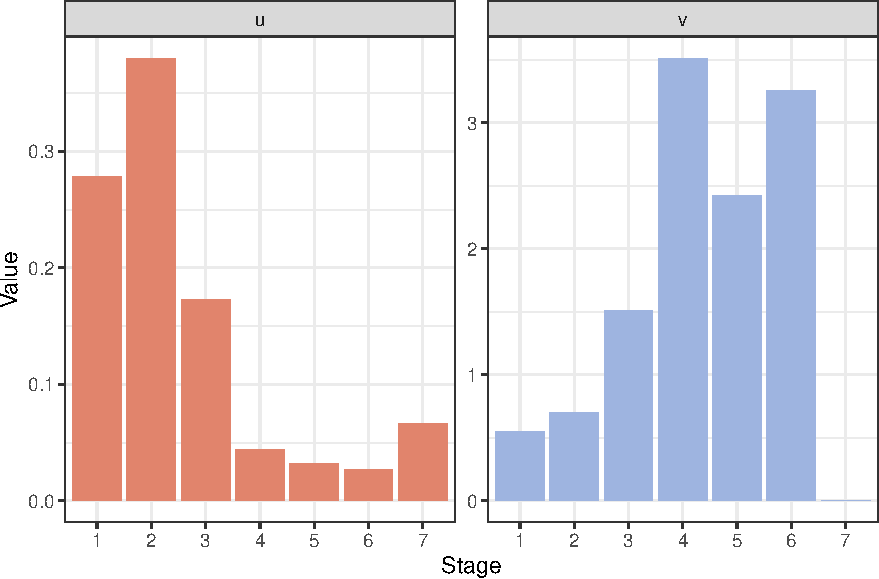
\includegraphics{DemographyCompendium_files/figure-latex/unnamed-chunk-76-1.pdf}

The growth rate is \(\lambda\approx\) 1.0745 per month. Per year the growth rate is \(\lambda^12\approx\) 2.3683. Thus, the annual growth rate is high, more than doubling the population each year. However, this matrix model assumes that the population can reproduce every month, and reaches a stable structure with individuals in the reproductive stages each month, while in reality there are only two main breeding periods per year \citep{Kammenga1}. Thus, while the model can describe the life of one cohort reasonably well (e.g.~we can use the projection matrix to project the growth over a year or two starting with a cohort in stage 1), it likely overestimates the population growth rate.

Note that the reproductive value is zero in the final stage, because this is a post-reproductive stage. It does not contribute to population growth, but can still be relevant to consider in the model.

\begin{enumerate}
\def\labelenumi{\arabic{enumi}.}
\setcounter{enumi}{3}
\tightlist
\item
  Write function that returns the projection matrix as a function of the input vectors:
\end{enumerate}

\begin{Shaded}
\begin{Highlighting}[]
\NormalTok{A.isopod }\OtherTok{\textless{}{-}} \ControlFlowTok{function}\NormalTok{(}\AttributeTok{PV=}\NormalTok{Pvec, }\AttributeTok{GV=}\NormalTok{Gvec, }\AttributeTok{FV=}\NormalTok{Fvec)\{}
\NormalTok{  Umat.isopod }\OtherTok{\textless{}{-}}\NormalTok{ Fmat.isopod }\OtherTok{\textless{}{-}} \FunctionTok{matrix}\NormalTok{(}\DecValTok{0}\NormalTok{,}\DecValTok{7}\NormalTok{,}\DecValTok{7}\NormalTok{)}
\NormalTok{  Umat.isopod[}\FunctionTok{row}\NormalTok{(Umat.isopod) }\SpecialCharTok{==} \FunctionTok{col}\NormalTok{(Umat.isopod) }\SpecialCharTok{+} \DecValTok{1}\NormalTok{] }\OtherTok{\textless{}{-}}\NormalTok{ GV[}\DecValTok{1}\SpecialCharTok{:}\DecValTok{6}\NormalTok{]}
\NormalTok{  Umat.isopod[}\FunctionTok{row}\NormalTok{(Umat.isopod) }\SpecialCharTok{==} \FunctionTok{col}\NormalTok{(Umat.isopod)] }\OtherTok{\textless{}{-}}\NormalTok{ PV}
\NormalTok{  Fmat.isopod[}\DecValTok{1}\NormalTok{,] }\OtherTok{\textless{}{-}}\NormalTok{ FV}
\NormalTok{  Amat.isopod }\OtherTok{\textless{}{-}}\NormalTok{ Umat.isopod }\SpecialCharTok{+}\NormalTok{ Fmat.isopod}
\NormalTok{  Amat.isopod}
\NormalTok{\}}
\end{Highlighting}
\end{Shaded}

What happens to \(\lambda\), \(\mathbf{u}\) and \(\mathbf{v}\) if you modify
the element \(G_6\) (here the element is multiplied by 0.5):

\begin{Shaded}
\begin{Highlighting}[]
\CommentTok{\#Modify element 6 of the G{-}vector, e.g. multiply it by 0.5}
\NormalTok{Amat.isopod2 }\OtherTok{\textless{}{-}} \FunctionTok{A.isopod}\NormalTok{(}\AttributeTok{GV=}\FunctionTok{c}\NormalTok{(}\FloatTok{0.722}\NormalTok{, }\FloatTok{0.244}\NormalTok{, }\FloatTok{0.231}\NormalTok{, }\FloatTok{0.788}\NormalTok{ , }\FloatTok{0.792}\NormalTok{, }\FloatTok{0.5}\SpecialCharTok{*}\FloatTok{0.664}\NormalTok{,}\DecValTok{0}\NormalTok{))}
\NormalTok{res.isopod2 }\OtherTok{\textless{}{-}} \FunctionTok{uvlambda}\NormalTok{(Amat.isopod2)}

\NormalTok{lambda.isopod2 }\OtherTok{\textless{}{-}}\NormalTok{ res.isopod2}\SpecialCharTok{$}\NormalTok{lam}

\CommentTok{\#Make a data frame for plotting:}
\NormalTok{resframe.isopod2 }\OtherTok{\textless{}{-}} \FunctionTok{data.frame}\NormalTok{(}\StringTok{"Stage"}\OtherTok{=}\FunctionTok{as.factor}\NormalTok{(}\DecValTok{1}\SpecialCharTok{:}\DecValTok{7}\NormalTok{), }\StringTok{"u"}\OtherTok{=}\NormalTok{res.isopod2}\SpecialCharTok{$}\NormalTok{u, }\StringTok{"v"}\OtherTok{=}\FunctionTok{as.vector}\NormalTok{(res.isopod2}\SpecialCharTok{$}\NormalTok{v))}

\CommentTok{\#Long format:}
\NormalTok{resframe.isopod.long2 }\OtherTok{\textless{}{-}}\NormalTok{ resframe.isopod2 }\SpecialCharTok{\%\textgreater{}\%} \FunctionTok{pivot\_longer}\NormalTok{(}\FunctionTok{c}\NormalTok{(u, v), }\AttributeTok{names\_to =} \StringTok{"uv"}\NormalTok{, }\AttributeTok{values\_to =} \StringTok{"Value"}\NormalTok{)}
 
\CommentTok{\#Plot with ggplot:}
\FunctionTok{ggplot}\NormalTok{(resframe.isopod.long2) }\SpecialCharTok{+} 
  \FunctionTok{geom\_col}\NormalTok{(}\FunctionTok{aes}\NormalTok{(}\AttributeTok{x=}\NormalTok{Stage, }\AttributeTok{y=}\NormalTok{Value, }\AttributeTok{fill=}\NormalTok{uv ))}\SpecialCharTok{+}
  \FunctionTok{scale\_fill\_manual}\NormalTok{(}\AttributeTok{values=}\NormalTok{colors2)}\SpecialCharTok{+}
  \FunctionTok{facet\_wrap}\NormalTok{(}\SpecialCharTok{\textasciitilde{}}\FunctionTok{factor}\NormalTok{(uv, }\AttributeTok{levels=}\FunctionTok{c}\NormalTok{(}\StringTok{"u"}\NormalTok{, }\StringTok{"v"}\NormalTok{)), }\AttributeTok{scales=}\StringTok{"free"}\NormalTok{)}\SpecialCharTok{+}
  \FunctionTok{theme\_bw}\NormalTok{() }\SpecialCharTok{+}
  \FunctionTok{labs}\NormalTok{( }\AttributeTok{x=}\StringTok{"Stage"}\NormalTok{, }\AttributeTok{y=}\StringTok{"Value"}\NormalTok{)}\SpecialCharTok{+}
  \FunctionTok{theme}\NormalTok{(}\AttributeTok{legend.position =} \StringTok{"none"}\NormalTok{ ) }
\end{Highlighting}
\end{Shaded}

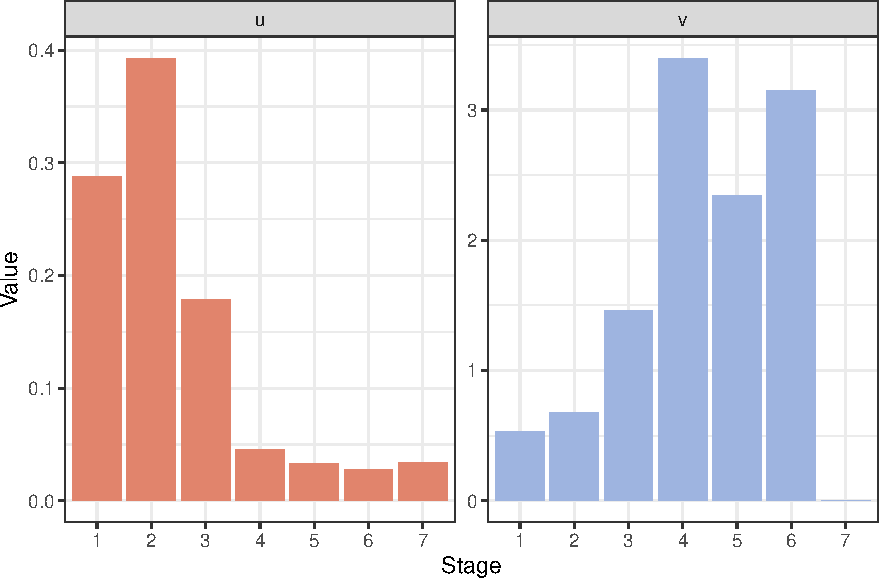
\includegraphics{DemographyCompendium_files/figure-latex/unnamed-chunk-78-1.pdf}

If we use a new value of \(G_6=0.5\cdot 0.664\) (half the original), we get \(\lambda\approx\) 1.0745, exactly the same as before. This is because only the final stage is affected, which is a post-reproductive stage not contributing to population growth. The stable structure changes slightly because we get relatively fewer individuals in the final stage. As a result the reproductive values are also rescaled but otherwise not changed.

\begin{enumerate}
\def\labelenumi{\arabic{enumi}.}
\setcounter{enumi}{4}
\tightlist
\item
  Modify the element \(G_4\) instead:
\end{enumerate}

\begin{Shaded}
\begin{Highlighting}[]
\CommentTok{\#Modify element 6 of the G{-}vector, e.g. multiply it by 0.5}
\NormalTok{Amat.isopod3 }\OtherTok{\textless{}{-}} \FunctionTok{A.isopod}\NormalTok{(}\AttributeTok{GV=}\FunctionTok{c}\NormalTok{(}\FloatTok{0.722}\NormalTok{, }\FloatTok{0.244}\NormalTok{, }\FloatTok{0.231}\NormalTok{, }\FloatTok{0.5}\SpecialCharTok{*}\FloatTok{0.788}\NormalTok{ , }\FloatTok{0.792}\NormalTok{, }\FloatTok{0.664}\NormalTok{,}\DecValTok{0}\NormalTok{))}
\NormalTok{res.isopod3 }\OtherTok{\textless{}{-}} \FunctionTok{uvlambda}\NormalTok{(Amat.isopod3)}

\NormalTok{lambda.isopod3 }\OtherTok{\textless{}{-}}\NormalTok{ res.isopod3}\SpecialCharTok{$}\NormalTok{lam}

\CommentTok{\#Make a data frame for plotting:}
\NormalTok{resframe.isopod3 }\OtherTok{\textless{}{-}} \FunctionTok{data.frame}\NormalTok{(}\StringTok{"Stage"}\OtherTok{=}\FunctionTok{as.factor}\NormalTok{(}\DecValTok{1}\SpecialCharTok{:}\DecValTok{7}\NormalTok{), }\StringTok{"u"}\OtherTok{=}\NormalTok{res.isopod3}\SpecialCharTok{$}\NormalTok{u, }\StringTok{"v"}\OtherTok{=}\FunctionTok{as.vector}\NormalTok{(res.isopod3}\SpecialCharTok{$}\NormalTok{v))}

\CommentTok{\#Long format:}
\NormalTok{resframe.isopod.long3 }\OtherTok{\textless{}{-}}\NormalTok{ resframe.isopod3 }\SpecialCharTok{\%\textgreater{}\%} \FunctionTok{pivot\_longer}\NormalTok{(}\FunctionTok{c}\NormalTok{(u, v), }\AttributeTok{names\_to =} \StringTok{"uv"}\NormalTok{, }\AttributeTok{values\_to =} \StringTok{"Value"}\NormalTok{)}
 

\CommentTok{\#Plot with ggplot:}
\FunctionTok{ggplot}\NormalTok{(resframe.isopod.long3) }\SpecialCharTok{+} 
  \FunctionTok{geom\_col}\NormalTok{(}\FunctionTok{aes}\NormalTok{(}\AttributeTok{x=}\NormalTok{Stage, }\AttributeTok{y=}\NormalTok{Value, }\AttributeTok{fill=}\NormalTok{uv ))}\SpecialCharTok{+}
  \FunctionTok{scale\_fill\_manual}\NormalTok{(}\AttributeTok{values=}\NormalTok{colors2)}\SpecialCharTok{+}
  \FunctionTok{facet\_wrap}\NormalTok{(}\SpecialCharTok{\textasciitilde{}}\FunctionTok{factor}\NormalTok{(uv, }\AttributeTok{levels=}\FunctionTok{c}\NormalTok{(}\StringTok{"u"}\NormalTok{, }\StringTok{"v"}\NormalTok{)), }\AttributeTok{scales=}\StringTok{"free"}\NormalTok{)}\SpecialCharTok{+}
  \FunctionTok{theme\_bw}\NormalTok{() }\SpecialCharTok{+}
  \FunctionTok{labs}\NormalTok{( }\AttributeTok{x=}\StringTok{"Stage"}\NormalTok{, }\AttributeTok{y=}\StringTok{"Value"}\NormalTok{)}\SpecialCharTok{+}
  \FunctionTok{theme}\NormalTok{(}\AttributeTok{legend.position =} \StringTok{"none"}\NormalTok{ ) }
\end{Highlighting}
\end{Shaded}

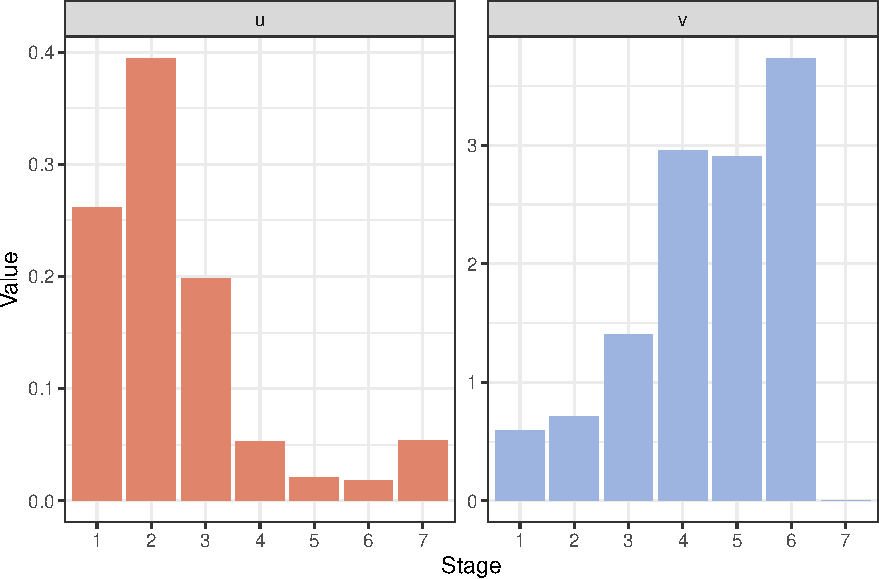
\includegraphics{DemographyCompendium_files/figure-latex/unnamed-chunk-79-1.pdf}

If we use a new value of \(G_4=0.5\cdot 0.788\) (half the original), we get \(\lambda\approx\) 1.0246, lower than before. This time the second reproductive stage is also affected, as fewer individuals transition out from stage 4. The highest reproductive value shifts to stage 6 instead of 4, but there are fewer individuals reaching this stage than before.

\hypertarget{exercise-4.3-1}{%
\subsection*{Exercise 4.3}\label{exercise-4.3-1}}
\addcontentsline{toc}{subsection}{Exercise 4.3}

\begin{enumerate}
\def\labelenumi{\arabic{enumi}.}
\tightlist
\item
  To define the new matrix \(\mathbf{A}_C\) we can use the function defined in exercise 4.2 returning the projection matrix as a function of the vectors \(P\), \(G\), and \(F\):
\end{enumerate}

\begin{Shaded}
\begin{Highlighting}[]
\NormalTok{PvecC }\OtherTok{\textless{}{-}} \FunctionTok{c}\NormalTok{(}\FloatTok{0.158}\NormalTok{, }\FloatTok{0.507}\NormalTok{, }\FloatTok{0.501}\NormalTok{, }\FloatTok{0.15}\NormalTok{, }\FloatTok{0.007}\NormalTok{, }\FloatTok{0.126}\NormalTok{, }\FloatTok{0.744}\NormalTok{)}
\NormalTok{GvecC }\OtherTok{\textless{}{-}} \FunctionTok{c}\NormalTok{(}\FloatTok{0.722}\NormalTok{, }\FloatTok{0.228}\NormalTok{, }\FloatTok{0.215}\NormalTok{, }\FloatTok{0.733}\NormalTok{, }\FloatTok{0.737}\NormalTok{, }\FloatTok{0.618}\NormalTok{,}\DecValTok{0}\NormalTok{)}
\NormalTok{FvecC }\OtherTok{\textless{}{-}} \FunctionTok{c}\NormalTok{(}\DecValTok{0}\NormalTok{, }\DecValTok{0}\NormalTok{, }\DecValTok{0}\NormalTok{, }\FloatTok{2.355}\NormalTok{, }\DecValTok{0}\NormalTok{,}\DecValTok{0}\NormalTok{,}\DecValTok{0}\NormalTok{)}
 
\NormalTok{Amat.isopod.C }\OtherTok{\textless{}{-}} \FunctionTok{A.isopod}\NormalTok{(}\AttributeTok{PV=}\NormalTok{PvecC, }\AttributeTok{GV=}\NormalTok{GvecC, }\AttributeTok{FV=}\NormalTok{FvecC)}
\end{Highlighting}
\end{Shaded}

\begin{enumerate}
\def\labelenumi{\arabic{enumi}.}
\setcounter{enumi}{1}
\tightlist
\item
  Calculate \(\lambda\) for the new matrix:
\end{enumerate}

\begin{Shaded}
\begin{Highlighting}[]
\NormalTok{res.isopod.C }\OtherTok{\textless{}{-}} \FunctionTok{uvlambda}\NormalTok{(Amat.isopod.C)}
\NormalTok{lambda.isopod.C }\OtherTok{\textless{}{-}}\NormalTok{ res.isopod.C}\SpecialCharTok{$}\NormalTok{lam}
\end{Highlighting}
\end{Shaded}

The value of \(\lambda\) in the `cadmium environment' is \(\lambda\approx\) 0.8941, much lower than the reference values of \(\lambda_R\approx\) 1.0745 (exercise 4.2). The difference in \(\lambda\) is \(\lambda_C-\lambda_R\approx round(lambda.isopod.C-lambda.isopod,4)\).

\begin{enumerate}
\def\labelenumi{\arabic{enumi}.}
\setcounter{enumi}{2}
\tightlist
\item
  Calculate halfway and difference matrix:
\end{enumerate}

\begin{Shaded}
\begin{Highlighting}[]
\CommentTok{\#Amat.isopod from previous exercise.}
\NormalTok{Halfway.matrix.isopod }\OtherTok{\textless{}{-}} \FloatTok{0.5}\SpecialCharTok{*}\NormalTok{(Amat.isopod.C}\SpecialCharTok{+}\NormalTok{Amat.isopod)}

\NormalTok{Difference.matrix.isopod }\OtherTok{\textless{}{-}}\NormalTok{ (Amat.isopod.C}\SpecialCharTok{{-}}\NormalTok{Amat.isopod)}
\end{Highlighting}
\end{Shaded}

\begin{enumerate}
\def\labelenumi{\arabic{enumi}.}
\setcounter{enumi}{3}
\tightlist
\item
  Calculate sensitivity matrix and calculate / plot LTRE contributions:
\end{enumerate}

\begin{Shaded}
\begin{Highlighting}[]
\CommentTok{\#Modify element 6 of the G{-}vector, e.g. multiply it by 0.5}
\NormalTok{Sensitivity.Halfway.isopod }\OtherTok{\textless{}{-}} \FunctionTok{sensitivity.matrix}\NormalTok{(Halfway.matrix.isopod)}

\NormalTok{LTRE.matrix.isopod }\OtherTok{\textless{}{-}} \FunctionTok{sensitivity.matrix}\NormalTok{(Halfway.matrix.isopod)}\SpecialCharTok{*}\NormalTok{Difference.matrix.isopod}

\CommentTok{\#Extract components corresponding to G, P, and F across stages:}
\NormalTok{LTRE\_F }\OtherTok{\textless{}{-}}\NormalTok{ LTRE.matrix.isopod[}\DecValTok{1}\NormalTok{,] }
\NormalTok{LTRE\_P }\OtherTok{\textless{}{-}} \FunctionTok{c}\NormalTok{(}\FunctionTok{diag}\NormalTok{(LTRE.matrix.isopod[}\DecValTok{2}\SpecialCharTok{:}\DecValTok{7}\NormalTok{,}\DecValTok{1}\SpecialCharTok{:}\DecValTok{6}\NormalTok{]),}\DecValTok{0}\NormalTok{)}
\NormalTok{LTRE\_G }\OtherTok{\textless{}{-}} \FunctionTok{diag}\NormalTok{(LTRE.matrix.isopod)}
  

\CommentTok{\#Make a data frame for plotting:}
\NormalTok{LTREframe }\OtherTok{\textless{}{-}} \FunctionTok{data.frame}\NormalTok{(}\StringTok{"Stage"}\OtherTok{=}\FunctionTok{as.factor}\NormalTok{(}\DecValTok{1}\SpecialCharTok{:}\DecValTok{7}\NormalTok{), }\StringTok{"Gcont"}\OtherTok{=}\NormalTok{LTRE\_G, }\StringTok{"Pcont"}\OtherTok{=}\NormalTok{LTRE\_P, }\StringTok{"Fcont"}\OtherTok{=}\NormalTok{LTRE\_F)}

\CommentTok{\#Long format:}
\NormalTok{LTREframe.long }\OtherTok{\textless{}{-}}\NormalTok{ LTREframe }\SpecialCharTok{\%\textgreater{}\%} \FunctionTok{pivot\_longer}\NormalTok{(}\FunctionTok{c}\NormalTok{(Gcont, Pcont, Fcont), }\AttributeTok{names\_to =} \StringTok{"Contribution"}\NormalTok{, }\AttributeTok{values\_to =} \StringTok{"Value"}\NormalTok{)}
 

\CommentTok{\#Plot with ggplot:}
\FunctionTok{ggplot}\NormalTok{(LTREframe.long) }\SpecialCharTok{+} 
  \FunctionTok{geom\_col}\NormalTok{(}\FunctionTok{aes}\NormalTok{(}\AttributeTok{x=}\NormalTok{Stage, }\AttributeTok{y=}\NormalTok{Value, }\AttributeTok{fill=}\NormalTok{Contribution ))}\SpecialCharTok{+}
  \FunctionTok{scale\_fill\_manual}\NormalTok{(}\AttributeTok{values=}\NormalTok{colors3)}\SpecialCharTok{+}
  \FunctionTok{facet\_wrap}\NormalTok{(}\SpecialCharTok{\textasciitilde{}}\FunctionTok{factor}\NormalTok{(Contribution, }\AttributeTok{levels=}\FunctionTok{c}\NormalTok{(}\StringTok{"Gcont"}\NormalTok{, }\StringTok{"Pcont"}\NormalTok{, }\StringTok{"Fcont"}\NormalTok{)), }\AttributeTok{scales=}\StringTok{"free"}\NormalTok{)}\SpecialCharTok{+}
  \FunctionTok{theme\_bw}\NormalTok{() }\SpecialCharTok{+}
  \FunctionTok{labs}\NormalTok{( }\AttributeTok{x=}\StringTok{"Stage"}\NormalTok{, }\AttributeTok{y=}\StringTok{"Value"}\NormalTok{)}\SpecialCharTok{+}
  \FunctionTok{theme}\NormalTok{(}\AttributeTok{legend.position =} \StringTok{"none"}\NormalTok{ ) }
\end{Highlighting}
\end{Shaded}

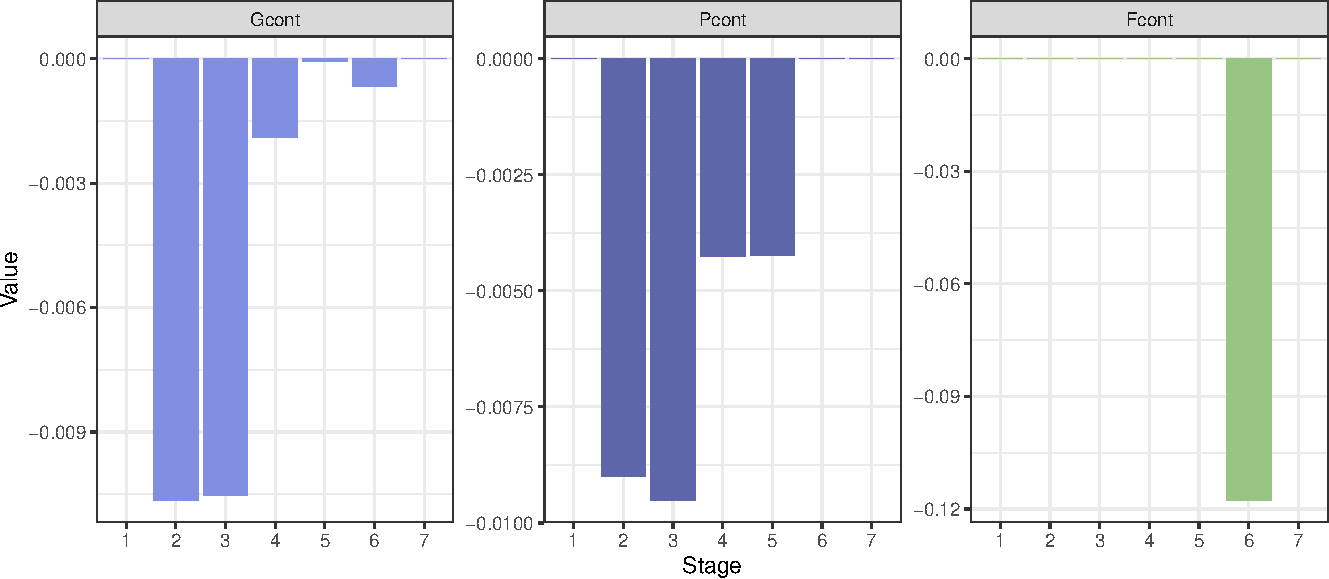
\includegraphics{DemographyCompendium_files/figure-latex/unnamed-chunk-83-1.pdf}

The contributions to \(\lambda_C-\lambda_R\approx\) -0.1804 are highest from \(P\) and \(G\) of stage 2 and 3, and from fertility of stage 6. The sum of contributions is \(\sum_{i,j}D_{ij}S^*_{ij}\approx\) -0.1687, a bit lower than the actual difference.

\begin{enumerate}
\def\labelenumi{\arabic{enumi}.}
\setcounter{enumi}{4}
\tightlist
\item
  LTRE is better if we want to understand the difference in \(\lambda\) in two different environments (or here, treatments), more specifically which parts of the projection matrix contribute to this difference. A sensitivity analysis applies to one environment and tells us how \(\lambda\) would respond to small perturbations in each matrix element. The sensitivity analysis is prospective, while the LTRE analysis is retrospective \citep{Caswell1}.
\end{enumerate}

\hypertarget{chapter-5-exercises}{%
\section{Chapter 5 exercises}\label{chapter-5-exercises}}

\hypertarget{exercise-5.1-1}{%
\subsection*{Exercise 5.1}\label{exercise-5.1-1}}
\addcontentsline{toc}{subsection}{Exercise 5.1}

\begin{enumerate}
\def\labelenumi{\arabic{enumi}.}
\tightlist
\item
  Add stochasticity to the fecundity coefficients, make plots:
\end{enumerate}

\begin{Shaded}
\begin{Highlighting}[]
\CommentTok{\#Project growth, variance 0.1}
\NormalTok{stochastic.plant }\OtherTok{\textless{}{-}} \FunctionTok{projection.stochastic}\NormalTok{(}\AttributeTok{Amats =} \FunctionTok{Amat.array}\NormalTok{(}\AttributeTok{MatA=}\NormalTok{APlant, }\AttributeTok{MatU=}\NormalTok{UPlant, }\AttributeTok{MatF=}\NormalTok{FPlant, }\AttributeTok{tmax=}\DecValTok{30}\NormalTok{, }\AttributeTok{VarF=}\FunctionTok{rep}\NormalTok{(}\FloatTok{0.1}\NormalTok{, }\DecValTok{4}\NormalTok{), }\AttributeTok{VarS=}\FunctionTok{rep}\NormalTok{(}\DecValTok{0}\NormalTok{, }\DecValTok{4}\NormalTok{)), }\AttributeTok{n0=}\FunctionTok{c}\NormalTok{(}\FunctionTok{rep}\NormalTok{(}\DecValTok{10}\NormalTok{,}\DecValTok{4}\NormalTok{)))}

\NormalTok{stochastic.plant}\SpecialCharTok{$}\NormalTok{varF }\OtherTok{\textless{}{-}}  \StringTok{"0.1"}

\CommentTok{\#Project growth, variance 0.01}
\NormalTok{stochastic.plant2 }\OtherTok{\textless{}{-}} \FunctionTok{projection.stochastic}\NormalTok{(}\AttributeTok{Amats =} \FunctionTok{Amat.array}\NormalTok{(}\AttributeTok{MatA=}\NormalTok{APlant, }\AttributeTok{MatU=}\NormalTok{UPlant, }\AttributeTok{MatF=}\NormalTok{FPlant, }\AttributeTok{tmax=}\DecValTok{30}\NormalTok{, }\AttributeTok{VarF=}\FunctionTok{rep}\NormalTok{(}\FloatTok{0.01}\NormalTok{, }\DecValTok{4}\NormalTok{), }\AttributeTok{VarS=}\FunctionTok{rep}\NormalTok{(}\DecValTok{0}\NormalTok{, }\DecValTok{4}\NormalTok{)), }\AttributeTok{n0=}\FunctionTok{c}\NormalTok{(}\FunctionTok{rep}\NormalTok{(}\DecValTok{10}\NormalTok{,}\DecValTok{4}\NormalTok{)))}

\NormalTok{stochastic.plant2}\SpecialCharTok{$}\NormalTok{varF }\OtherTok{\textless{}{-}}  \StringTok{"0.01"}


\CommentTok{\#Add the two:}
\NormalTok{stochastic.plant }\OtherTok{\textless{}{-}} \FunctionTok{rbind}\NormalTok{(stochastic.plant, stochastic.plant2) }


\CommentTok{\#Long format for plotting:}
\NormalTok{stochastic.plant.long }\OtherTok{\textless{}{-}}\NormalTok{ stochastic.plant }\SpecialCharTok{\%\textgreater{}\%} \FunctionTok{pivot\_longer}\NormalTok{(}\FunctionTok{c}\NormalTok{(}\SpecialCharTok{{-}}\NormalTok{time,}\SpecialCharTok{{-}}\NormalTok{varF),}
               \AttributeTok{names\_to =} \StringTok{"AgeClass"}\NormalTok{, }\AttributeTok{values\_to =} \StringTok{"Value"}\NormalTok{)}

\CommentTok{\#Plot:}
\FunctionTok{ggplot}\NormalTok{(stochastic.plant.long) }\SpecialCharTok{+} 
  \FunctionTok{geom\_line}\NormalTok{(}\FunctionTok{aes}\NormalTok{(}\AttributeTok{x=}\NormalTok{time, }\AttributeTok{y=}\NormalTok{Value, }\AttributeTok{col=}\NormalTok{AgeClass, }\AttributeTok{linetype=}\NormalTok{AgeClass), }\AttributeTok{lwd=}\FloatTok{1.2}\NormalTok{)}\SpecialCharTok{+}
  \FunctionTok{geom\_point}\NormalTok{(}\FunctionTok{aes}\NormalTok{(}\AttributeTok{x=}\NormalTok{time, }\AttributeTok{y=}\NormalTok{Value, }\AttributeTok{col=}\NormalTok{AgeClass), }\AttributeTok{size=}\DecValTok{3}\NormalTok{)}\SpecialCharTok{+}
  \FunctionTok{theme\_bw}\NormalTok{() }\SpecialCharTok{+}
   \FunctionTok{facet\_wrap}\NormalTok{(}\SpecialCharTok{\textasciitilde{}}\FunctionTok{factor}\NormalTok{(varF, }\AttributeTok{levels=}\FunctionTok{c}\NormalTok{(}\StringTok{"0.1"}\NormalTok{, }\StringTok{"0.01"}\NormalTok{)))}\SpecialCharTok{+}
  \FunctionTok{scale\_color\_manual}\NormalTok{(}\AttributeTok{values=}\NormalTok{colors4)}\SpecialCharTok{+} 
  \FunctionTok{scale\_linetype\_manual}\NormalTok{(}\AttributeTok{values=}\DecValTok{1}\SpecialCharTok{:}\DecValTok{4}\NormalTok{)}\SpecialCharTok{+}  
  \FunctionTok{labs}\NormalTok{( }\AttributeTok{x=}\StringTok{"Time (year)"}\NormalTok{, }\AttributeTok{y=}\StringTok{"Age class size"}\NormalTok{)  }\SpecialCharTok{+}
    \FunctionTok{theme}\NormalTok{(}\AttributeTok{legend.position =} \StringTok{"top"}\NormalTok{ ) }
\end{Highlighting}
\end{Shaded}

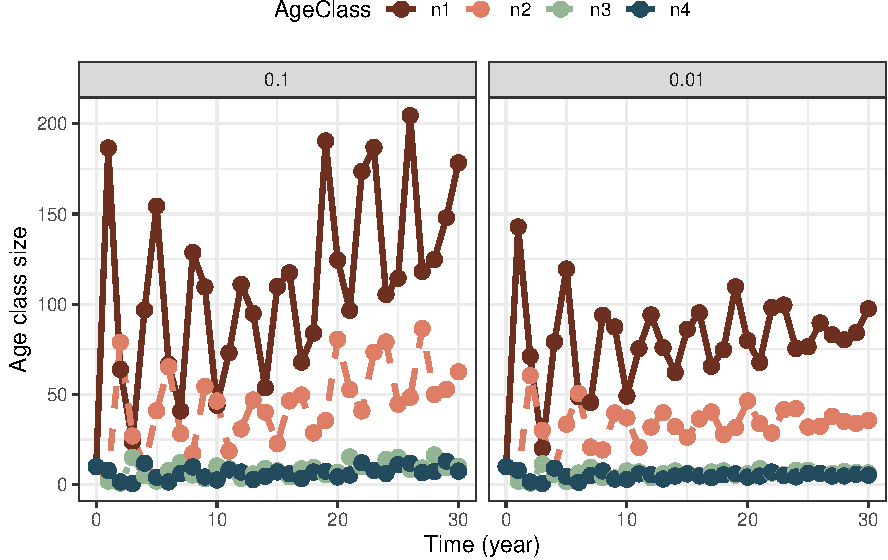
\includegraphics{DemographyCompendium_files/figure-latex/unnamed-chunk-85-1.pdf}

Variance in fertility increases the fluctuations in particular of the first age class. Note that we still have transient fluctuations in the beginning on top of the stochastic fluctuations. In the second case with lower variance in fertility, the variance in stage structure stabilizes at a lower value as well.

\begin{enumerate}
\def\labelenumi{\arabic{enumi}.}
\setcounter{enumi}{1}
\tightlist
\item
  Add stochasticity to the survival coefficients instead:
\end{enumerate}

\begin{Shaded}
\begin{Highlighting}[]
\CommentTok{\#Project growth, variance 0.1}
\NormalTok{stochastic.plant }\OtherTok{\textless{}{-}} \FunctionTok{projection.stochastic}\NormalTok{(}\AttributeTok{Amats =} \FunctionTok{Amat.array}\NormalTok{(}\AttributeTok{MatA=}\NormalTok{APlant, }\AttributeTok{MatU=}\NormalTok{UPlant, }\AttributeTok{MatF=}\NormalTok{FPlant, }\AttributeTok{tmax=}\DecValTok{30}\NormalTok{, }\AttributeTok{VarF=}\FunctionTok{rep}\NormalTok{(}\DecValTok{0}\NormalTok{, }\DecValTok{4}\NormalTok{), }\AttributeTok{VarS=}\FunctionTok{rep}\NormalTok{(}\FloatTok{0.1}\NormalTok{, }\DecValTok{4}\NormalTok{)), }\AttributeTok{n0=}\FunctionTok{c}\NormalTok{(}\FunctionTok{rep}\NormalTok{(}\DecValTok{10}\NormalTok{,}\DecValTok{4}\NormalTok{)))}

\NormalTok{stochastic.plant}\SpecialCharTok{$}\NormalTok{varS }\OtherTok{\textless{}{-}}  \StringTok{"0.1"}

\CommentTok{\#Project growth, variance 0.01}
\NormalTok{stochastic.plant2 }\OtherTok{\textless{}{-}} \FunctionTok{projection.stochastic}\NormalTok{(}\AttributeTok{Amats =} \FunctionTok{Amat.array}\NormalTok{(}\AttributeTok{MatA=}\NormalTok{APlant, }\AttributeTok{MatU=}\NormalTok{UPlant, }\AttributeTok{MatF=}\NormalTok{FPlant, }\AttributeTok{tmax=}\DecValTok{30}\NormalTok{, }\AttributeTok{VarF=}\FunctionTok{rep}\NormalTok{(}\DecValTok{0}\NormalTok{, }\DecValTok{4}\NormalTok{), }\AttributeTok{VarS=}\FunctionTok{rep}\NormalTok{(}\FloatTok{0.01}\NormalTok{, }\DecValTok{4}\NormalTok{)), }\AttributeTok{n0=}\FunctionTok{c}\NormalTok{(}\FunctionTok{rep}\NormalTok{(}\DecValTok{10}\NormalTok{,}\DecValTok{4}\NormalTok{)))}

\NormalTok{stochastic.plant2}\SpecialCharTok{$}\NormalTok{varS }\OtherTok{\textless{}{-}}  \StringTok{"0.01"}


\CommentTok{\#Add the two:}
\NormalTok{stochastic.plant }\OtherTok{\textless{}{-}} \FunctionTok{rbind}\NormalTok{(stochastic.plant, stochastic.plant2) }


\CommentTok{\#Long format for plotting:}
\NormalTok{stochastic.plant.long }\OtherTok{\textless{}{-}}\NormalTok{ stochastic.plant }\SpecialCharTok{\%\textgreater{}\%} \FunctionTok{pivot\_longer}\NormalTok{(}\FunctionTok{c}\NormalTok{(}\SpecialCharTok{{-}}\NormalTok{time,}\SpecialCharTok{{-}}\NormalTok{varS),}
               \AttributeTok{names\_to =} \StringTok{"AgeClass"}\NormalTok{, }\AttributeTok{values\_to =} \StringTok{"Value"}\NormalTok{)}

\CommentTok{\#Plot:}
\FunctionTok{ggplot}\NormalTok{(stochastic.plant.long) }\SpecialCharTok{+} 
  \FunctionTok{geom\_line}\NormalTok{(}\FunctionTok{aes}\NormalTok{(}\AttributeTok{x=}\NormalTok{time, }\AttributeTok{y=}\NormalTok{Value, }\AttributeTok{col=}\NormalTok{AgeClass, }\AttributeTok{linetype=}\NormalTok{AgeClass), }\AttributeTok{lwd=}\FloatTok{1.2}\NormalTok{)}\SpecialCharTok{+}
  \FunctionTok{geom\_point}\NormalTok{(}\FunctionTok{aes}\NormalTok{(}\AttributeTok{x=}\NormalTok{time, }\AttributeTok{y=}\NormalTok{Value, }\AttributeTok{col=}\NormalTok{AgeClass), }\AttributeTok{size=}\DecValTok{3}\NormalTok{)}\SpecialCharTok{+}
  \FunctionTok{theme\_bw}\NormalTok{() }\SpecialCharTok{+}
   \FunctionTok{facet\_wrap}\NormalTok{(}\SpecialCharTok{\textasciitilde{}}\FunctionTok{factor}\NormalTok{(varS, }\AttributeTok{levels=}\FunctionTok{c}\NormalTok{(}\StringTok{"0.1"}\NormalTok{, }\StringTok{"0.01"}\NormalTok{)))}\SpecialCharTok{+}
  \FunctionTok{scale\_color\_manual}\NormalTok{(}\AttributeTok{values=}\NormalTok{colors4)}\SpecialCharTok{+} 
  \FunctionTok{scale\_linetype\_manual}\NormalTok{(}\AttributeTok{values=}\DecValTok{1}\SpecialCharTok{:}\DecValTok{4}\NormalTok{)}\SpecialCharTok{+}  
  \FunctionTok{labs}\NormalTok{( }\AttributeTok{x=}\StringTok{"Time (year)"}\NormalTok{, }\AttributeTok{y=}\StringTok{"Age class size"}\NormalTok{)  }\SpecialCharTok{+}
   \FunctionTok{theme}\NormalTok{(}\AttributeTok{legend.position =} \StringTok{"top"}\NormalTok{ ) }
\end{Highlighting}
\end{Shaded}

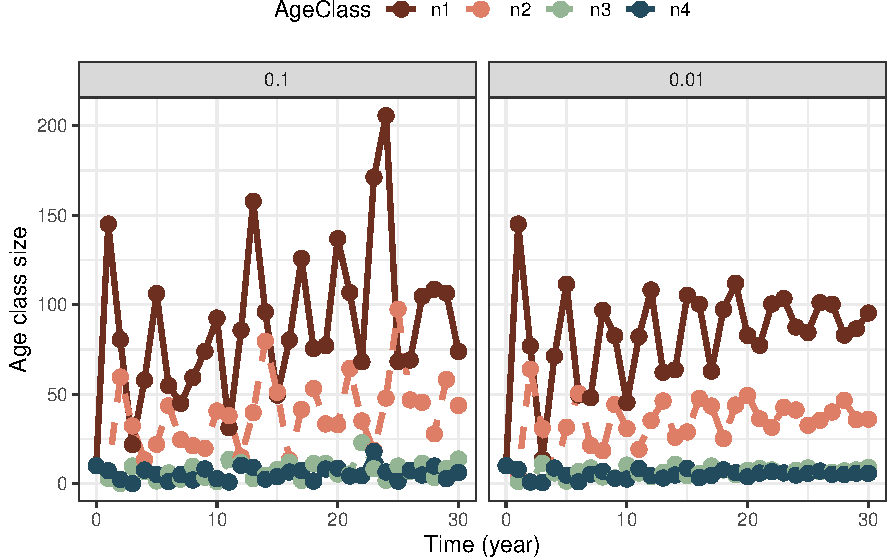
\includegraphics{DemographyCompendium_files/figure-latex/unnamed-chunk-86-1.pdf}

We get quite similar patterns with variance on survival coefficients instead of fertility. This is because any fluctuations in one age class are carried on to the next, and to offspring. We always get more variation in the offspring class, because this is the largest class.

\begin{enumerate}
\def\labelenumi{\arabic{enumi}.}
\setcounter{enumi}{2}
\tightlist
\item
  There are many potential ways a plant like this could show bet-hedging strategies, for instance:
\end{enumerate}

\begin{itemize}
\item
  Conservative bet-hedging (`play it safe'): Reduce the mean fecundity to increase mean survival. This could mean that the plant might reduce annual variance in fitness, at the cost of not being able to maximize reproduction in good years.
\item
  Diversifying bet-hedging (`don't put all eggs in one basket'): Spreading the risk among offspring (here seeds), either through different phenotypes, different spatial habitats, or different hatching times. The latter can be achieved through a seed bank, where seeds can lay dormant for many years before germinating.
\end{itemize}

A seed bank is a complicating factor to include in matrix models, but could be achieved by adding a new stage for the dormant seeds, with a certain probability of hatching each year. This would turn the model into a stage structured model.

One could argue that the plant life history already shows some bet-hedging since it reproduces at two ages, thus spreading the risk of reproducing at least among two years. Iteroparity can be interpreted as a bet-hedging strategy, but strictly speaking we would have to prove a cost to the arithmetic mean fitness to call it bet-hedging (e.g.~lowering the maximum number of offspring that can be produced in good years).

\hypertarget{exercise-5.2-1}{%
\subsection*{Exercise 5.2}\label{exercise-5.2-1}}
\addcontentsline{toc}{subsection}{Exercise 5.2}

\begin{enumerate}
\def\labelenumi{\arabic{enumi}.}
\tightlist
\item
  Calculate \(\lambda\) for each habitat:
\end{enumerate}

\begin{Shaded}
\begin{Highlighting}[]
\CommentTok{\#Create the Leslie matrices}
\NormalTok{AmatPoor }\OtherTok{\textless{}{-}} \FunctionTok{Create.Amat}\NormalTok{(}\AttributeTok{Svec=}\FunctionTok{c}\NormalTok{(.}\DecValTok{8}\NormalTok{,}\FunctionTok{rep}\NormalTok{(.}\DecValTok{82}\NormalTok{,}\DecValTok{4}\NormalTok{)),}\AttributeTok{Fvec=}\FunctionTok{c}\NormalTok{(}\DecValTok{0}\NormalTok{, }\FloatTok{0.1}\NormalTok{, }\FloatTok{0.16}\NormalTok{, }\FloatTok{0.2}\NormalTok{, }\FloatTok{0.2}\NormalTok{) )}

\NormalTok{AmatGood }\OtherTok{\textless{}{-}} \FunctionTok{Create.Amat}\NormalTok{(}\AttributeTok{Svec=}\FunctionTok{c}\NormalTok{(.}\DecValTok{8}\NormalTok{,}\FunctionTok{rep}\NormalTok{(.}\DecValTok{82}\NormalTok{,}\DecValTok{4}\NormalTok{)),}\AttributeTok{Fvec=}\FunctionTok{c}\NormalTok{(}\DecValTok{0}\NormalTok{, }\FloatTok{0.096}\NormalTok{, }\FloatTok{0.16}\NormalTok{, }\FloatTok{0.224}\NormalTok{, }\FloatTok{0.32}\NormalTok{)  )}
 
 
\CommentTok{\#Calculate lambda:}

\NormalTok{lambda.good }\OtherTok{\textless{}{-}} \FunctionTok{uvlambda}\NormalTok{(AmatGood)}\SpecialCharTok{$}\NormalTok{lam}
\NormalTok{lambda.poor }\OtherTok{\textless{}{-}} \FunctionTok{uvlambda}\NormalTok{(AmatPoor)}\SpecialCharTok{$}\NormalTok{lam}

\NormalTok{lambda.habitats }\OtherTok{\textless{}{-}} \FunctionTok{data.frame}\NormalTok{(}\StringTok{"lambda.good"}\OtherTok{=}\NormalTok{lambda.good, }\StringTok{"lambda.poor"}\OtherTok{=}\NormalTok{lambda.poor)}

\NormalTok{lambda.habitats}
\end{Highlighting}
\end{Shaded}

\begin{verbatim}
##   lambda.good lambda.poor
## 1     1.01092   0.9682986
\end{verbatim}

We see that \(\lambda>1\) in the good habitat, and \(\lambda<1\) in the poor habitat. This calculation assumes no connection between them, treating each as a separate population (what would hypothetically happen to each over time with no migration between them).

\begin{enumerate}
\def\labelenumi{\arabic{enumi}.}
\setcounter{enumi}{1}
\tightlist
\item
  Generate sequence of matrices returned as array:
\end{enumerate}

\begin{Shaded}
\begin{Highlighting}[]
\NormalTok{ArrayFunction }\OtherTok{\textless{}{-}} \ControlFlowTok{function}\NormalTok{(}\AttributeTok{Agood=}\NormalTok{AmatGood, }\AttributeTok{Apoor=}\NormalTok{AmatPoor, }\AttributeTok{time=}\DecValTok{30}\NormalTok{)\{}
  \CommentTok{\#Generate sequence of good or bad habitat years:}
\NormalTok{  random.sequence }\OtherTok{\textless{}{-}} \FunctionTok{sample}\NormalTok{(}\FunctionTok{c}\NormalTok{(}\StringTok{"Good"}\NormalTok{, }\StringTok{"Poor"}\NormalTok{), time, }\AttributeTok{replace=}\ConstantTok{TRUE}\NormalTok{)}
  \CommentTok{\#Generate empty array:}
\NormalTok{  k }\OtherTok{\textless{}{-}} \FunctionTok{dim}\NormalTok{(Agood)[}\DecValTok{1}\NormalTok{]}
\NormalTok{  A.array }\OtherTok{\textless{}{-}} \FunctionTok{array}\NormalTok{(}\ConstantTok{NA}\NormalTok{, }\AttributeTok{dim=}\FunctionTok{c}\NormalTok{(k,k,time))}
  \CommentTok{\#Fill in right matrix depending on the sequence}
  \ControlFlowTok{for}\NormalTok{(i }\ControlFlowTok{in} \DecValTok{1}\SpecialCharTok{:}\NormalTok{time)\{}
    \ControlFlowTok{if}\NormalTok{(random.sequence[i]}\SpecialCharTok{==}\StringTok{"Good"}\NormalTok{)\{}
\NormalTok{      A.array[,,i] }\OtherTok{\textless{}{-}}\NormalTok{ Agood}
\NormalTok{    \}}
    \ControlFlowTok{else}\NormalTok{ \{}
\NormalTok{       A.array[,,i] }\OtherTok{\textless{}{-}}\NormalTok{ Apoor}
\NormalTok{    \}}
\NormalTok{  \}}
\NormalTok{  A.array}
\NormalTok{\}}

\CommentTok{\#Test:}
\FunctionTok{ArrayFunction}\NormalTok{(}\AttributeTok{time=}\DecValTok{10}\NormalTok{)}
\end{Highlighting}
\end{Shaded}

\begin{verbatim}
## , , 1
## 
##      [,1] [,2] [,3] [,4] [,5]
## [1,]  0.0 0.10 0.16 0.20 0.20
## [2,]  0.8 0.00 0.00 0.00 0.00
## [3,]  0.0 0.82 0.00 0.00 0.00
## [4,]  0.0 0.00 0.82 0.00 0.00
## [5,]  0.0 0.00 0.00 0.82 0.82
## 
## , , 2
## 
##      [,1]  [,2] [,3]  [,4] [,5]
## [1,]  0.0 0.096 0.16 0.224 0.32
## [2,]  0.8 0.000 0.00 0.000 0.00
## [3,]  0.0 0.820 0.00 0.000 0.00
## [4,]  0.0 0.000 0.82 0.000 0.00
## [5,]  0.0 0.000 0.00 0.820 0.82
## 
## , , 3
## 
##      [,1]  [,2] [,3]  [,4] [,5]
## [1,]  0.0 0.096 0.16 0.224 0.32
## [2,]  0.8 0.000 0.00 0.000 0.00
## [3,]  0.0 0.820 0.00 0.000 0.00
## [4,]  0.0 0.000 0.82 0.000 0.00
## [5,]  0.0 0.000 0.00 0.820 0.82
## 
## , , 4
## 
##      [,1]  [,2] [,3]  [,4] [,5]
## [1,]  0.0 0.096 0.16 0.224 0.32
## [2,]  0.8 0.000 0.00 0.000 0.00
## [3,]  0.0 0.820 0.00 0.000 0.00
## [4,]  0.0 0.000 0.82 0.000 0.00
## [5,]  0.0 0.000 0.00 0.820 0.82
## 
## , , 5
## 
##      [,1]  [,2] [,3]  [,4] [,5]
## [1,]  0.0 0.096 0.16 0.224 0.32
## [2,]  0.8 0.000 0.00 0.000 0.00
## [3,]  0.0 0.820 0.00 0.000 0.00
## [4,]  0.0 0.000 0.82 0.000 0.00
## [5,]  0.0 0.000 0.00 0.820 0.82
## 
## , , 6
## 
##      [,1] [,2] [,3] [,4] [,5]
## [1,]  0.0 0.10 0.16 0.20 0.20
## [2,]  0.8 0.00 0.00 0.00 0.00
## [3,]  0.0 0.82 0.00 0.00 0.00
## [4,]  0.0 0.00 0.82 0.00 0.00
## [5,]  0.0 0.00 0.00 0.82 0.82
## 
## , , 7
## 
##      [,1] [,2] [,3] [,4] [,5]
## [1,]  0.0 0.10 0.16 0.20 0.20
## [2,]  0.8 0.00 0.00 0.00 0.00
## [3,]  0.0 0.82 0.00 0.00 0.00
## [4,]  0.0 0.00 0.82 0.00 0.00
## [5,]  0.0 0.00 0.00 0.82 0.82
## 
## , , 8
## 
##      [,1] [,2] [,3] [,4] [,5]
## [1,]  0.0 0.10 0.16 0.20 0.20
## [2,]  0.8 0.00 0.00 0.00 0.00
## [3,]  0.0 0.82 0.00 0.00 0.00
## [4,]  0.0 0.00 0.82 0.00 0.00
## [5,]  0.0 0.00 0.00 0.82 0.82
## 
## , , 9
## 
##      [,1] [,2] [,3] [,4] [,5]
## [1,]  0.0 0.10 0.16 0.20 0.20
## [2,]  0.8 0.00 0.00 0.00 0.00
## [3,]  0.0 0.82 0.00 0.00 0.00
## [4,]  0.0 0.00 0.82 0.00 0.00
## [5,]  0.0 0.00 0.00 0.82 0.82
## 
## , , 10
## 
##      [,1] [,2] [,3] [,4] [,5]
## [1,]  0.0 0.10 0.16 0.20 0.20
## [2,]  0.8 0.00 0.00 0.00 0.00
## [3,]  0.0 0.82 0.00 0.00 0.00
## [4,]  0.0 0.00 0.82 0.00 0.00
## [5,]  0.0 0.00 0.00 0.82 0.82
\end{verbatim}

\begin{enumerate}
\def\labelenumi{\arabic{enumi}.}
\setcounter{enumi}{2}
\tightlist
\item
  The mean growth rate corresponds (in this case) to the growth rate \(\lambda_m\) of the mean matrix:
\end{enumerate}

\begin{Shaded}
\begin{Highlighting}[]
\NormalTok{MeanMatrix }\OtherTok{\textless{}{-}}\NormalTok{ (AmatPoor}\SpecialCharTok{+}\NormalTok{AmatGood)}\SpecialCharTok{/}\DecValTok{2}
\NormalTok{r.mean }\OtherTok{\textless{}{-}} \FunctionTok{log}\NormalTok{(}\FunctionTok{uvlambda}\NormalTok{(MeanMatrix)}\SpecialCharTok{$}\NormalTok{lambda)}
\end{Highlighting}
\end{Shaded}

Stochastic growth rate:

\begin{Shaded}
\begin{Highlighting}[]
\NormalTok{AMATS}\OtherTok{\textless{}{-}}\FunctionTok{ArrayFunction}\NormalTok{(}\AttributeTok{time=}\DecValTok{10000}\NormalTok{)}
\NormalTok{rs.gull }\OtherTok{\textless{}{-}} \FunctionTok{EstimateSGR}\NormalTok{(}\AttributeTok{Amats =}\NormalTok{ AMATS, }\AttributeTok{n0=}\FunctionTok{rep}\NormalTok{(}\DecValTok{10}\NormalTok{,}\DecValTok{5}\NormalTok{))}
\end{Highlighting}
\end{Shaded}

For the gulls the mean growth rate is \(r\approx\) -0.0089, while the stochastic growth rate is \(r_s\approx\) -0.0089. Both are negative, the stochastic growth rate sligtly lower.

To make a quantile plot we perform a large number of stochastic simulations as described in the chapter and shown for the songbird example, after modifying the \texttt{nsim.stochastic} function to include the new random process of generating an array of matrices:

\begin{Shaded}
\begin{Highlighting}[]
\NormalTok{nsim.stochastic.gull }\OtherTok{\textless{}{-}} \ControlFlowTok{function}\NormalTok{(}\AttributeTok{Agood=}\NormalTok{AmatGood, }\AttributeTok{Apoor=}\NormalTok{AmatPoor, }\AttributeTok{tmax=}\DecValTok{30}\NormalTok{, }\AttributeTok{nsim=}\DecValTok{1000}\NormalTok{,}\AttributeTok{n0=}\FunctionTok{rep}\NormalTok{(}\DecValTok{10}\NormalTok{,}\DecValTok{5}\NormalTok{))\{}
\NormalTok{  frame }\OtherTok{\textless{}{-}}  \FunctionTok{data.frame}\NormalTok{(}\StringTok{"Time"}\OtherTok{=}\DecValTok{0}\SpecialCharTok{:}\NormalTok{tmax)}
  \ControlFlowTok{for}\NormalTok{(m }\ControlFlowTok{in} \DecValTok{1}\SpecialCharTok{:}\NormalTok{nsim)\{}
\NormalTok{    AMATS }\OtherTok{\textless{}{-}} \FunctionTok{ArrayFunction}\NormalTok{(}\AttributeTok{Agood=}\NormalTok{Agood, }\AttributeTok{Apoor=}\NormalTok{Apoor, }\AttributeTok{time=}\NormalTok{tmax)}
\NormalTok{    projectN }\OtherTok{\textless{}{-}} \FunctionTok{apply}\NormalTok{(}\FunctionTok{projection.stochastic}\NormalTok{(}\AttributeTok{Amats=}\NormalTok{AMATS, }\AttributeTok{n0=}\NormalTok{n0)[,}\SpecialCharTok{{-}}\DecValTok{1}\NormalTok{],}\DecValTok{1}\NormalTok{,sum)}
\NormalTok{    frame }\OtherTok{\textless{}{-}} \FunctionTok{cbind}\NormalTok{(frame, projectN)}
     \FunctionTok{names}\NormalTok{(frame)[m}\SpecialCharTok{+}\DecValTok{1}\NormalTok{] }\OtherTok{\textless{}{-}} \FunctionTok{paste}\NormalTok{(}\StringTok{"Rep"}\NormalTok{,m,}\AttributeTok{sep=}\StringTok{""}\NormalTok{)}
\NormalTok{  \}}
\NormalTok{  frame}
\NormalTok{\}}

\CommentTok{\#Apply function to get 10 0000 realizations (can take some time)}
\NormalTok{simgull\_Large }\OtherTok{\textless{}{-}} \FunctionTok{nsim.stochastic.gull}\NormalTok{(}\AttributeTok{nsim=}\DecValTok{10000}\NormalTok{)}

\CommentTok{\#Get the 5, 25, 50, 75, and 95 percentiles:}
\NormalTok{PercentilesGull  }\OtherTok{\textless{}{-}} \FunctionTok{t}\NormalTok{(}\FunctionTok{apply}\NormalTok{(}\FunctionTok{t}\NormalTok{(simgull\_Large[,}\SpecialCharTok{{-}}\DecValTok{1}\NormalTok{]),}\DecValTok{2}\NormalTok{, quantile, }\AttributeTok{probs=}\FunctionTok{c}\NormalTok{(.}\DecValTok{05}\NormalTok{, .}\DecValTok{25}\NormalTok{, .}\DecValTok{5}\NormalTok{, .}\DecValTok{75}\NormalTok{,.}\DecValTok{95}\NormalTok{)))}

 
\CommentTok{\#Store percentiles in data frame  }
\NormalTok{GullPercentiles }\OtherTok{\textless{}{-}} \FunctionTok{as.data.frame}\NormalTok{(}\FunctionTok{cbind}\NormalTok{(}\StringTok{"Time"}\OtherTok{=}\DecValTok{0}\SpecialCharTok{:}\NormalTok{(}\FunctionTok{dim}\NormalTok{(PercentilesGull)[}\DecValTok{1}\NormalTok{]}\SpecialCharTok{{-}}\DecValTok{1}\NormalTok{),  PercentilesGull))}

\NormalTok{GullPercentiles}\SpecialCharTok{$}\NormalTok{Mean }\OtherTok{\textless{}{-}} \FunctionTok{apply}\NormalTok{(}\FunctionTok{t}\NormalTok{(simgull\_Large[,}\SpecialCharTok{{-}}\DecValTok{1}\NormalTok{]),}\DecValTok{2}\NormalTok{, mean)}

\CommentTok{\#Make long format for plotting}
\NormalTok{GullPercentiles.long }\OtherTok{\textless{}{-}}\NormalTok{ GullPercentiles }\SpecialCharTok{\%\textgreater{}\%} \FunctionTok{pivot\_longer}\NormalTok{(}\FunctionTok{c}\NormalTok{(}\SpecialCharTok{{-}}\NormalTok{Time),}
               \AttributeTok{names\_to =} \StringTok{"Percentile"}\NormalTok{, }\AttributeTok{values\_to =} \StringTok{"N"}\NormalTok{)}

\CommentTok{\#Make sure the order of the percentiles is correct}
\NormalTok{GullPercentiles.long}\SpecialCharTok{$}\NormalTok{Percentile }\OtherTok{\textless{}{-}} \FunctionTok{factor}\NormalTok{(GullPercentiles.long}\SpecialCharTok{$}\NormalTok{Percentile, }\AttributeTok{levels=}\FunctionTok{c}\NormalTok{(}\StringTok{"5\%"}\NormalTok{, }\StringTok{"25\%"}\NormalTok{, }\StringTok{"50\%"}\NormalTok{, }\StringTok{"75\%"}\NormalTok{, }\StringTok{"95\%"}\NormalTok{,}\StringTok{"Mean"}\NormalTok{))}

\FunctionTok{ggplot}\NormalTok{(GullPercentiles.long) }\SpecialCharTok{+} 
  \FunctionTok{geom\_line}\NormalTok{(}\FunctionTok{aes}\NormalTok{(}\AttributeTok{x=}\NormalTok{Time, }\AttributeTok{y=}\NormalTok{N, }\AttributeTok{col=}\NormalTok{Percentile,}\AttributeTok{linetype=}\NormalTok{Percentile), }\AttributeTok{lwd=}\DecValTok{1}\NormalTok{)}\SpecialCharTok{+}
  \FunctionTok{scale\_color\_manual}\NormalTok{(}\AttributeTok{values=}\FunctionTok{c}\NormalTok{(colors5,}\DecValTok{2}\NormalTok{))}\SpecialCharTok{+}
   \FunctionTok{scale\_linetype\_manual}\NormalTok{(}\AttributeTok{values=}\FunctionTok{c}\NormalTok{(}\FunctionTok{rep}\NormalTok{(}\DecValTok{1}\NormalTok{,}\DecValTok{5}\NormalTok{),}\DecValTok{2}\NormalTok{))}\SpecialCharTok{+}
  \FunctionTok{theme\_bw}\NormalTok{() }\SpecialCharTok{+}
   \FunctionTok{theme}\NormalTok{(}\AttributeTok{legend.position =} \StringTok{"top"}\NormalTok{,}\AttributeTok{legend.title =} \FunctionTok{element\_blank}\NormalTok{() )}\SpecialCharTok{+}
  \FunctionTok{labs}\NormalTok{( }\AttributeTok{x=}\StringTok{"Time (year)"}\NormalTok{, }\AttributeTok{y=}\StringTok{"Population size N"}\NormalTok{) }\SpecialCharTok{+}
   \FunctionTok{guides}\NormalTok{(}\AttributeTok{color =} \FunctionTok{guide\_legend}\NormalTok{(}\AttributeTok{nrow =} \DecValTok{1}\NormalTok{, }\AttributeTok{byrow =} \ConstantTok{TRUE}\NormalTok{))}
\end{Highlighting}
\end{Shaded}

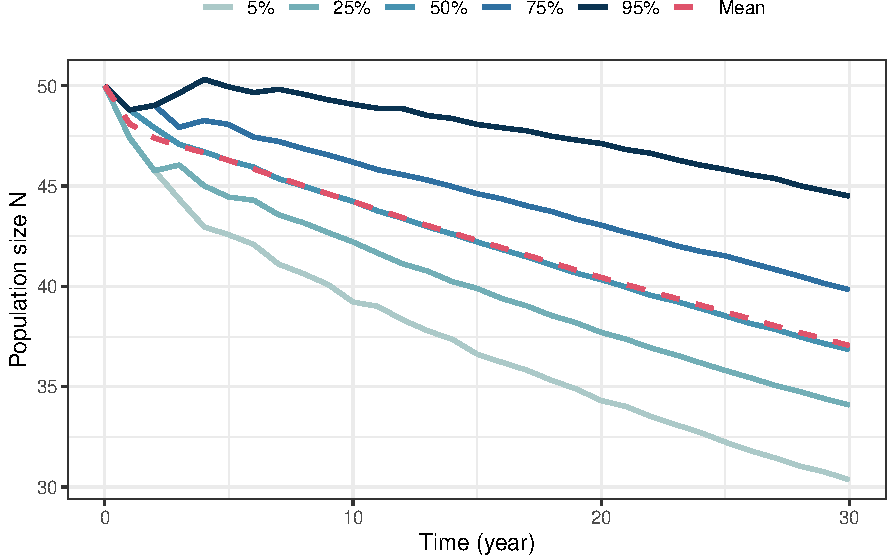
\includegraphics{DemographyCompendium_files/figure-latex/unnamed-chunk-91-1.pdf}

\begin{enumerate}
\def\labelenumi{\arabic{enumi}.}
\setcounter{enumi}{3}
\tightlist
\item
\end{enumerate}

First we add the probability argument to the function generating a random sequence of projection matrices:

\begin{Shaded}
\begin{Highlighting}[]
\CommentTok{\#}
\NormalTok{ArrayFunction }\OtherTok{\textless{}{-}} \ControlFlowTok{function}\NormalTok{(}\AttributeTok{Agood=}\NormalTok{AmatGood, }\AttributeTok{Apoor=}\NormalTok{AmatPoor, }\AttributeTok{time=}\DecValTok{30}\NormalTok{, }\AttributeTok{prob=}\FunctionTok{c}\NormalTok{(.}\DecValTok{5}\NormalTok{,.}\DecValTok{5}\NormalTok{))\{}
  \CommentTok{\#Generate sequence of good or bad habitat years:}
\NormalTok{  random.sequence }\OtherTok{\textless{}{-}} \FunctionTok{sample}\NormalTok{(}\FunctionTok{c}\NormalTok{(}\StringTok{"Good"}\NormalTok{, }\StringTok{"Poor"}\NormalTok{), time, }\AttributeTok{replace=}\ConstantTok{TRUE}\NormalTok{, }\AttributeTok{prob=}\NormalTok{prob)}
  \CommentTok{\#Generate empty array:}
\NormalTok{  k }\OtherTok{\textless{}{-}} \FunctionTok{dim}\NormalTok{(Agood)[}\DecValTok{1}\NormalTok{]}
\NormalTok{  A.array }\OtherTok{\textless{}{-}} \FunctionTok{array}\NormalTok{(}\ConstantTok{NA}\NormalTok{, }\AttributeTok{dim=}\FunctionTok{c}\NormalTok{(k,k,time))}
  \CommentTok{\#Fill in right matrix depending on the sequence}
  \ControlFlowTok{for}\NormalTok{(i }\ControlFlowTok{in} \DecValTok{1}\SpecialCharTok{:}\NormalTok{time)\{}
    \ControlFlowTok{if}\NormalTok{(random.sequence[i]}\SpecialCharTok{==}\StringTok{"Good"}\NormalTok{)\{}
\NormalTok{      A.array[,,i] }\OtherTok{\textless{}{-}}\NormalTok{ Agood}
\NormalTok{    \}}
    \ControlFlowTok{else}\NormalTok{ \{}
\NormalTok{       A.array[,,i] }\OtherTok{\textless{}{-}}\NormalTok{ Apoor}
\NormalTok{    \}}
\NormalTok{  \}}
\NormalTok{  A.array}
\NormalTok{\}}
\end{Highlighting}
\end{Shaded}

Then we modify the simulation function to include the argument

\begin{Shaded}
\begin{Highlighting}[]
\NormalTok{nsim.stochastic.gull }\OtherTok{\textless{}{-}} \ControlFlowTok{function}\NormalTok{(}\AttributeTok{Agood=}\NormalTok{AmatGood, }\AttributeTok{Apoor=}\NormalTok{AmatPoor, }\AttributeTok{tmax=}\DecValTok{30}\NormalTok{, }\AttributeTok{nsim=}\DecValTok{1000}\NormalTok{, }\AttributeTok{n0=}\FunctionTok{rep}\NormalTok{(}\DecValTok{10}\NormalTok{,}\DecValTok{5}\NormalTok{), }\AttributeTok{prob=}\FunctionTok{c}\NormalTok{(.}\DecValTok{5}\NormalTok{,.}\DecValTok{5}\NormalTok{))\{}
\NormalTok{  frame }\OtherTok{\textless{}{-}}  \FunctionTok{data.frame}\NormalTok{(}\StringTok{"Time"}\OtherTok{=}\DecValTok{0}\SpecialCharTok{:}\NormalTok{tmax)}
  \ControlFlowTok{for}\NormalTok{(m }\ControlFlowTok{in} \DecValTok{1}\SpecialCharTok{:}\NormalTok{nsim)\{}
\NormalTok{    AMATS }\OtherTok{\textless{}{-}} \FunctionTok{ArrayFunction}\NormalTok{(}\AttributeTok{Agood=}\NormalTok{Agood, }\AttributeTok{Apoor=}\NormalTok{Apoor, }\AttributeTok{time=}\NormalTok{tmax, }\AttributeTok{prob=}\NormalTok{prob)}
\NormalTok{    projectN }\OtherTok{\textless{}{-}} \FunctionTok{apply}\NormalTok{(}\FunctionTok{projection.stochastic}\NormalTok{(}\AttributeTok{Amats=}\NormalTok{AMATS, }\AttributeTok{n0=}\NormalTok{n0)[,}\SpecialCharTok{{-}}\DecValTok{1}\NormalTok{],}\DecValTok{1}\NormalTok{,sum)}
\NormalTok{    frame }\OtherTok{\textless{}{-}} \FunctionTok{cbind}\NormalTok{(frame, projectN)}
     \FunctionTok{names}\NormalTok{(frame)[m}\SpecialCharTok{+}\DecValTok{1}\NormalTok{] }\OtherTok{\textless{}{-}} \FunctionTok{paste}\NormalTok{(}\StringTok{"Rep"}\NormalTok{,m,}\AttributeTok{sep=}\StringTok{""}\NormalTok{)}
\NormalTok{  \}}
\NormalTok{  frame}
\NormalTok{\}}
\end{Highlighting}
\end{Shaded}

Now we can apply the function to compare situations where the probability of drawing a good environment is (e.g.) 0.8, versus 0.2:

\begin{Shaded}
\begin{Highlighting}[]
\CommentTok{\#Most good environments}
\NormalTok{simgullG }\OtherTok{\textless{}{-}} \FunctionTok{nsim.stochastic.gull}\NormalTok{(}\AttributeTok{nsim=}\DecValTok{10000}\NormalTok{, }\AttributeTok{prob=}\FunctionTok{c}\NormalTok{(.}\DecValTok{8}\NormalTok{,.}\DecValTok{2}\NormalTok{))}
\CommentTok{\#Most poor environments}
\NormalTok{simgullP }\OtherTok{\textless{}{-}} \FunctionTok{nsim.stochastic.gull}\NormalTok{(}\AttributeTok{nsim=}\DecValTok{10000}\NormalTok{, }\AttributeTok{prob=}\FunctionTok{c}\NormalTok{(.}\DecValTok{2}\NormalTok{,.}\DecValTok{8}\NormalTok{))}

\CommentTok{\#Get the 5, 25, 50, 75, and 95 percentiles:}
\NormalTok{PercentilesG  }\OtherTok{\textless{}{-}} \FunctionTok{t}\NormalTok{(}\FunctionTok{apply}\NormalTok{(}\FunctionTok{t}\NormalTok{(simgullG[,}\SpecialCharTok{{-}}\DecValTok{1}\NormalTok{]),}\DecValTok{2}\NormalTok{, quantile, }\AttributeTok{probs=}\FunctionTok{c}\NormalTok{(.}\DecValTok{05}\NormalTok{, .}\DecValTok{25}\NormalTok{, .}\DecValTok{5}\NormalTok{, .}\DecValTok{75}\NormalTok{,.}\DecValTok{95}\NormalTok{)))}
\NormalTok{PercentilesP  }\OtherTok{\textless{}{-}} \FunctionTok{t}\NormalTok{(}\FunctionTok{apply}\NormalTok{(}\FunctionTok{t}\NormalTok{(simgullP[,}\SpecialCharTok{{-}}\DecValTok{1}\NormalTok{]),}\DecValTok{2}\NormalTok{, quantile, }\AttributeTok{probs=}\FunctionTok{c}\NormalTok{(.}\DecValTok{05}\NormalTok{, .}\DecValTok{25}\NormalTok{, .}\DecValTok{5}\NormalTok{, .}\DecValTok{75}\NormalTok{,.}\DecValTok{95}\NormalTok{)))}

\CommentTok{\#Store percentiles in data frame  }
\NormalTok{GPercentiles }\OtherTok{\textless{}{-}} \FunctionTok{as.data.frame}\NormalTok{(}\FunctionTok{cbind}\NormalTok{(}\StringTok{"Time"}\OtherTok{=}\DecValTok{0}\SpecialCharTok{:}\NormalTok{(}\FunctionTok{dim}\NormalTok{(PercentilesG)[}\DecValTok{1}\NormalTok{]}\SpecialCharTok{{-}}\DecValTok{1}\NormalTok{),  PercentilesG))}
\NormalTok{GPercentiles}\SpecialCharTok{$}\NormalTok{Mean }\OtherTok{\textless{}{-}} \FunctionTok{apply}\NormalTok{(}\FunctionTok{t}\NormalTok{(PercentilesG[,}\SpecialCharTok{{-}}\DecValTok{1}\NormalTok{]),}\DecValTok{2}\NormalTok{, mean)}

\NormalTok{PPercentiles }\OtherTok{\textless{}{-}} \FunctionTok{as.data.frame}\NormalTok{(}\FunctionTok{cbind}\NormalTok{(}\StringTok{"Time"}\OtherTok{=}\DecValTok{0}\SpecialCharTok{:}\NormalTok{(}\FunctionTok{dim}\NormalTok{(PercentilesP)[}\DecValTok{1}\NormalTok{]}\SpecialCharTok{{-}}\DecValTok{1}\NormalTok{),  PercentilesP))}
\NormalTok{PPercentiles}\SpecialCharTok{$}\NormalTok{Mean }\OtherTok{\textless{}{-}} \FunctionTok{apply}\NormalTok{(}\FunctionTok{t}\NormalTok{(PercentilesP[,}\SpecialCharTok{{-}}\DecValTok{1}\NormalTok{]),}\DecValTok{2}\NormalTok{, mean)}

\CommentTok{\#Add probability value}
\NormalTok{GPercentiles}\SpecialCharTok{$}\NormalTok{ProbGood }\OtherTok{\textless{}{-}} \StringTok{"ProbGood\_0.8"}
\NormalTok{PPercentiles}\SpecialCharTok{$}\NormalTok{ProbGood }\OtherTok{\textless{}{-}} \StringTok{"ProbGood\_0.2"}

\CommentTok{\#Join:}

\NormalTok{PercentilesBoth }\OtherTok{\textless{}{-}} \FunctionTok{rbind}\NormalTok{(GPercentiles, PPercentiles)}

\CommentTok{\#Make long format for plotting}
\NormalTok{PercentilesBoth.long }\OtherTok{\textless{}{-}}\NormalTok{ PercentilesBoth }\SpecialCharTok{\%\textgreater{}\%} \FunctionTok{pivot\_longer}\NormalTok{(}\FunctionTok{c}\NormalTok{(}\SpecialCharTok{{-}}\NormalTok{Time, }\SpecialCharTok{{-}}\NormalTok{ProbGood),}
               \AttributeTok{names\_to =} \StringTok{"Percentile"}\NormalTok{, }\AttributeTok{values\_to =} \StringTok{"N"}\NormalTok{)}

\CommentTok{\#Make sure the order of the percentiles is correct}
\NormalTok{PercentilesBoth.long}\SpecialCharTok{$}\NormalTok{Percentile }\OtherTok{\textless{}{-}} \FunctionTok{factor}\NormalTok{(PercentilesBoth.long}\SpecialCharTok{$}\NormalTok{Percentile, }\AttributeTok{levels=}\FunctionTok{c}\NormalTok{(}\StringTok{"5\%"}\NormalTok{, }\StringTok{"25\%"}\NormalTok{, }\StringTok{"50\%"}\NormalTok{, }\StringTok{"75\%"}\NormalTok{, }\StringTok{"95\%"}\NormalTok{,}\StringTok{"Mean"}\NormalTok{))}

\FunctionTok{ggplot}\NormalTok{(PercentilesBoth.long) }\SpecialCharTok{+} 
  \FunctionTok{geom\_line}\NormalTok{(}\FunctionTok{aes}\NormalTok{(}\AttributeTok{x=}\NormalTok{Time, }\AttributeTok{y=}\NormalTok{N, }\AttributeTok{col=}\NormalTok{Percentile,}\AttributeTok{linetype=}\NormalTok{Percentile), }\AttributeTok{lwd=}\DecValTok{1}\NormalTok{)}\SpecialCharTok{+}
  \FunctionTok{scale\_color\_manual}\NormalTok{(}\AttributeTok{values=}\FunctionTok{c}\NormalTok{(colors5,}\DecValTok{2}\NormalTok{))}\SpecialCharTok{+}
   \FunctionTok{scale\_linetype\_manual}\NormalTok{(}\AttributeTok{values=}\FunctionTok{c}\NormalTok{(}\FunctionTok{rep}\NormalTok{(}\DecValTok{1}\NormalTok{,}\DecValTok{5}\NormalTok{),}\DecValTok{2}\NormalTok{))}\SpecialCharTok{+}
  \FunctionTok{theme\_bw}\NormalTok{() }\SpecialCharTok{+}
  \FunctionTok{ylim}\NormalTok{(}\DecValTok{0}\NormalTok{,}\DecValTok{80}\NormalTok{)}\SpecialCharTok{+}
  \FunctionTok{facet\_wrap}\NormalTok{(}\FunctionTok{vars}\NormalTok{(ProbGood),}\AttributeTok{ncol=}\DecValTok{2}\NormalTok{ ,}\AttributeTok{scales=}\StringTok{"free"}\NormalTok{)}\SpecialCharTok{+}
   \FunctionTok{theme}\NormalTok{(}\AttributeTok{legend.position =} \StringTok{"top"}\NormalTok{,}\AttributeTok{legend.title =} \FunctionTok{element\_blank}\NormalTok{() )}\SpecialCharTok{+}
  \FunctionTok{labs}\NormalTok{( }\AttributeTok{x=}\StringTok{"Time (year)"}\NormalTok{, }\AttributeTok{y=}\StringTok{"Population size N"}\NormalTok{) }\SpecialCharTok{+}
   \FunctionTok{guides}\NormalTok{(}\AttributeTok{color =} \FunctionTok{guide\_legend}\NormalTok{(}\AttributeTok{nrow =} \DecValTok{1}\NormalTok{, }\AttributeTok{byrow =} \ConstantTok{TRUE}\NormalTok{))}
\end{Highlighting}
\end{Shaded}

\includegraphics{DemographyCompendium_files/figure-latex/unnamed-chunk-94-1.pdf}

In the case where the probability of using the good environment increases (to the right), population growth is higher (perhaps not surprising).

\hypertarget{s07-Code-Collection}{%
\chapter{R code collection}\label{s07-Code-Collection}}

This appendix includes a collection of the R functions used in the compendium.

An RData-file containing all the functions as well as relevant R objects for the songbird example can be downloaded here:

To import this file into R, use \texttt{load("CompendiumCode.RData")} (after saving the file in your R working directory folder). Then all functions and objects should be visible in the `Environment' tab.

\hypertarget{life-tables}{%
\section{Life tables}\label{life-tables}}

\hypertarget{net-reproductive-rate-r_0}{%
\subsection{\texorpdfstring{Net reproductive rate \(R_0\)}{Net reproductive rate R\_0}}\label{net-reproductive-rate-r_0}}

\begin{Shaded}
\begin{Highlighting}[]
\NormalTok{R0.lifetable }\OtherTok{\textless{}{-}} \ControlFlowTok{function}\NormalTok{(lx, mx)\{}
  \FunctionTok{sum}\NormalTok{(lx}\SpecialCharTok{*}\NormalTok{mx) }
\NormalTok{\}}
\end{Highlighting}
\end{Shaded}

\hypertarget{euler-lotka}{%
\subsection{Euler-Lotka}\label{euler-lotka}}

Solving the equation for \(\lambda\) using \texttt{uniroot()}:

\begin{Shaded}
\begin{Highlighting}[]
\NormalTok{EulerLotka }\OtherTok{\textless{}{-}} \ControlFlowTok{function}\NormalTok{(lambda, x, lx, mx)\{}
  \FunctionTok{sum}\NormalTok{(lambda}\SpecialCharTok{\^{}}\NormalTok{(}\SpecialCharTok{{-}}\NormalTok{x)}\SpecialCharTok{*}\NormalTok{lx}\SpecialCharTok{*}\NormalTok{mx)}\SpecialCharTok{{-}}\DecValTok{1}
\NormalTok{\}}

\CommentTok{\#For application with uniroot, see e.g. the bird example in the text (chapter 2), or the plant example in exercises.}
\end{Highlighting}
\end{Shaded}

\hypertarget{matrix-population-models}{%
\section{Matrix population models}\label{matrix-population-models}}

\hypertarget{create-leslie-matrix}{%
\subsection{Create Leslie matrix}\label{create-leslie-matrix}}

Build Leslie matrix from vectors of survival and fertility coefficients (need to have same length). If the last survival coefficient is not zero, individuals can accumulate in the final class.

\begin{Shaded}
\begin{Highlighting}[]
\NormalTok{Create.Amat }\OtherTok{\textless{}{-}} \ControlFlowTok{function}\NormalTok{(Svec, Fvec)\{}
\NormalTok{  k }\OtherTok{\textless{}{-}} \FunctionTok{length}\NormalTok{(Svec)}
\NormalTok{  MatA}\OtherTok{\textless{}{-}} \FunctionTok{matrix}\NormalTok{(}\DecValTok{0}\NormalTok{,k,k)}
\NormalTok{  MatA[}\DecValTok{1}\NormalTok{,] }\OtherTok{\textless{}{-}}\NormalTok{ Fvec }
  \ControlFlowTok{for}\NormalTok{(i }\ControlFlowTok{in} \DecValTok{1}\SpecialCharTok{:}\NormalTok{(k}\DecValTok{{-}1}\NormalTok{))\{}
\NormalTok{    MatA[i}\SpecialCharTok{+}\DecValTok{1}\NormalTok{,i] }\OtherTok{\textless{}{-}}\NormalTok{ Svec[i]}
\NormalTok{  \}}
\NormalTok{  MatA[k,k] }\OtherTok{\textless{}{-}}\NormalTok{ Svec[k] }\CommentTok{\#Allow individuals to accumulate in final class if Svec[k] \textgreater{}0.}
\NormalTok{  MatA}
\NormalTok{  \}}
\end{Highlighting}
\end{Shaded}

\hypertarget{decompose-mathbfu-and-mathbff}{%
\subsection{\texorpdfstring{Decompose \(\mathbf{U}\) and \(\mathbf{F}\)}{Decompose \textbackslash mathbf\{U\} and \textbackslash mathbf\{F\}}}\label{decompose-mathbfu-and-mathbff}}

Decompose the matrices \(\mathbf{U}\) and \(\mathbf{F}\) based on equation to obtain the transition matrix \(\mathbf{G}\) vector of survival probability \(\mathbf{s}\) (from \(\mathbf{U}\)), and the transition matrix \(\mathbf{Q}\) the fertility vector \(\mathbf{f}\) (from \(\mathbf{F}\))

\begin{Shaded}
\begin{Highlighting}[]
\NormalTok{DecomposeU }\OtherTok{\textless{}{-}} \ControlFlowTok{function}\NormalTok{(MatU)\{}
\NormalTok{  k}\OtherTok{\textless{}{-}}\FunctionTok{dim}\NormalTok{(MatU)[}\DecValTok{1}\NormalTok{]}
  \ControlFlowTok{if}\NormalTok{(}\FunctionTok{is.na}\NormalTok{(MatU[k,k]))\{}
\NormalTok{    MatU[k,k]}\OtherTok{\textless{}{-}}\DecValTok{0}
\NormalTok{  \}}
\NormalTok{  Svec }\OtherTok{\textless{}{-}} \FunctionTok{apply}\NormalTok{(MatU,}\DecValTok{2}\NormalTok{,sum)}
\NormalTok{  MatG }\OtherTok{\textless{}{-}} \FunctionTok{t}\NormalTok{(}\FunctionTok{t}\NormalTok{(MatU)}\SpecialCharTok{/}\NormalTok{Svec)}
  \ControlFlowTok{for}\NormalTok{(i }\ControlFlowTok{in} \DecValTok{1}\SpecialCharTok{:}\NormalTok{k)\{}
    \ControlFlowTok{if}\NormalTok{(Svec[i]}\SpecialCharTok{==}\DecValTok{0}\NormalTok{)\{}
\NormalTok{      MatG[,i] }\OtherTok{\textless{}{-}} \DecValTok{0}
\NormalTok{      MatG[i,i] }\OtherTok{\textless{}{-}} \DecValTok{1}
\NormalTok{    \}}
\NormalTok{  \}}
 \FunctionTok{list}\NormalTok{(}\StringTok{"Gmat"}\OtherTok{=}\NormalTok{MatG,}\StringTok{"Survival"}\OtherTok{=}\NormalTok{Svec)}
\NormalTok{\}}
\end{Highlighting}
\end{Shaded}

\begin{Shaded}
\begin{Highlighting}[]
\NormalTok{DecomposeF }\OtherTok{\textless{}{-}} \ControlFlowTok{function}\NormalTok{(MatF)\{}
\NormalTok{    k }\OtherTok{\textless{}{-}} \FunctionTok{dim}\NormalTok{(MatF)[}\DecValTok{1}\NormalTok{]}
\NormalTok{    Fvec }\OtherTok{\textless{}{-}} \FunctionTok{apply}\NormalTok{(MatF,}\DecValTok{2}\NormalTok{,sum)}
\NormalTok{    MatQ }\OtherTok{\textless{}{-}} \FunctionTok{matrix}\NormalTok{(}\DecValTok{0}\NormalTok{,k,k)}
    \ControlFlowTok{for}\NormalTok{(i }\ControlFlowTok{in} \DecValTok{1}\SpecialCharTok{:}\NormalTok{k)\{}
        \ControlFlowTok{if}\NormalTok{(Fvec[i]}\SpecialCharTok{==}\DecValTok{0}\NormalTok{)\{}
\NormalTok{            MatQ[}\DecValTok{1}\NormalTok{,i]}\OtherTok{\textless{}{-}}\DecValTok{1}
            
\NormalTok{        \}}
        \ControlFlowTok{else}\NormalTok{\{}
\NormalTok{            MatQ[,i]}\OtherTok{\textless{}{-}}\NormalTok{MatF[,i]}\SpecialCharTok{/}\NormalTok{Fvec[i]}
\NormalTok{        \}}
\NormalTok{    \}}
 \FunctionTok{list}\NormalTok{(}\StringTok{"Qmat"}\OtherTok{=}\NormalTok{MatQ,}\StringTok{"Fertility"}\OtherTok{=}\NormalTok{Fvec)}
\NormalTok{\}}
\end{Highlighting}
\end{Shaded}

\hypertarget{population-projection}{%
\subsection{Population projection}\label{population-projection}}

Project size of stages over time given a projection matrix and an initial population vector. Return as data frame.

\begin{Shaded}
\begin{Highlighting}[]
\NormalTok{projection }\OtherTok{\textless{}{-}} \ControlFlowTok{function}\NormalTok{(MatA, }\AttributeTok{Tmax =} \DecValTok{50}\NormalTok{, n0)\{}
\NormalTok{  k }\OtherTok{\textless{}{-}} \FunctionTok{dim}\NormalTok{(MatA)[}\DecValTok{1}\NormalTok{]}
  \ControlFlowTok{if}\NormalTok{(}\FunctionTok{length}\NormalTok{(n0)}\SpecialCharTok{!=}\NormalTok{k)\{}
      \FunctionTok{warning}\NormalTok{(}\StringTok{"n0 should have length k corresponding to number of stages in Amat"}\NormalTok{)}
\NormalTok{      \}}
\NormalTok{  Nmat }\OtherTok{\textless{}{-}} \FunctionTok{matrix}\NormalTok{(}\ConstantTok{NA}\NormalTok{, }\AttributeTok{nrow=}\NormalTok{ Tmax}\SpecialCharTok{+}\DecValTok{1}\NormalTok{, }\AttributeTok{ncol=}\NormalTok{k)}
\NormalTok{  cnames }\OtherTok{\textless{}{-}} \FunctionTok{paste}\NormalTok{(}\StringTok{"n"}\NormalTok{, }\DecValTok{1}\SpecialCharTok{:}\NormalTok{k, }\AttributeTok{sep=}\StringTok{""}\NormalTok{)}
\NormalTok{  timesteps }\OtherTok{\textless{}{-}} \DecValTok{0}\SpecialCharTok{:}\NormalTok{Tmax}
\NormalTok{  Nmat[}\DecValTok{1}\NormalTok{,] }\OtherTok{=}\NormalTok{ n0 }
  \ControlFlowTok{for}\NormalTok{(i }\ControlFlowTok{in} \DecValTok{2}\SpecialCharTok{:}\NormalTok{(Tmax}\SpecialCharTok{+}\DecValTok{1}\NormalTok{))\{  }
\NormalTok{    Nmat[i,] }\OtherTok{=}\NormalTok{ MatA}\SpecialCharTok{\%*\%}\NormalTok{Nmat[i}\DecValTok{{-}1}\NormalTok{,]}
\NormalTok{  \}}
\NormalTok{  frame }\OtherTok{\textless{}{-}} \FunctionTok{data.frame}\NormalTok{(timesteps, Nmat)}
  \FunctionTok{colnames}\NormalTok{(frame) }\OtherTok{\textless{}{-}} \FunctionTok{c}\NormalTok{(}\StringTok{"time"}\NormalTok{, cnames)}
\NormalTok{  frame}
\NormalTok{\}}
\end{Highlighting}
\end{Shaded}

\hypertarget{long-term-growth-rate-stable-structure-and-reproductive-value}{%
\subsection{Long-term growth rate, stable structure and reproductive value}\label{long-term-growth-rate-stable-structure-and-reproductive-value}}

For a projection matrix \(\mathbf{A}\), the function returns the asymptotic growth rate \(\lambda\), a vector describing the stable stage structure \(\mathbf{u}\), and a vector describing the stage-specific reproductive values \(\mathbf{v}'\). NB: We scale the reproductive values so that \(\mathbf{v}'\mathbf{u}=1\).

\begin{Shaded}
\begin{Highlighting}[]
\NormalTok{uvlambda }\OtherTok{\textless{}{-}} \ControlFlowTok{function}\NormalTok{(MatA)\{}
\NormalTok{ ev }\OtherTok{\textless{}{-}} \FunctionTok{eigen}\NormalTok{(MatA)}
\NormalTok{ tev }\OtherTok{\textless{}{-}} \FunctionTok{eigen}\NormalTok{(}\FunctionTok{t}\NormalTok{(MatA))}
\NormalTok{ lmax }\OtherTok{\textless{}{-}} \FunctionTok{which.max}\NormalTok{(}\FunctionTok{Re}\NormalTok{(ev}\SpecialCharTok{$}\NormalTok{values))}
\NormalTok{ U }\OtherTok{\textless{}{-}}\NormalTok{ ev}\SpecialCharTok{$}\NormalTok{vectors}
\NormalTok{ V }\OtherTok{\textless{}{-}}\NormalTok{ tev}\SpecialCharTok{$}\NormalTok{vectors}
\NormalTok{ u }\OtherTok{\textless{}{-}} \FunctionTok{as.matrix}\NormalTok{(}\FunctionTok{abs}\NormalTok{(}\FunctionTok{Re}\NormalTok{(U[, lmax]))}\SpecialCharTok{/}\FunctionTok{sum}\NormalTok{(}\FunctionTok{abs}\NormalTok{(}\FunctionTok{Re}\NormalTok{(U[, lmax]))))}
\NormalTok{ u }\OtherTok{\textless{}{-}}\NormalTok{ u}\SpecialCharTok{/}\NormalTok{(}\FunctionTok{sum}\NormalTok{(u)) }\CommentTok{\#scale u}
\NormalTok{ v }\OtherTok{\textless{}{-}} \FunctionTok{as.matrix}\NormalTok{(}\FunctionTok{abs}\NormalTok{(}\FunctionTok{Re}\NormalTok{(V[, lmax])))}
\NormalTok{ v }\OtherTok{\textless{}{-}}\NormalTok{ v}\SpecialCharTok{/}\FunctionTok{sum}\NormalTok{(u}\SpecialCharTok{*}\NormalTok{v ) }\CommentTok{\#scale v}
\NormalTok{ v }\OtherTok{\textless{}{-}} \FunctionTok{t}\NormalTok{(}\FunctionTok{ifelse}\NormalTok{(u}\SpecialCharTok{*}\NormalTok{v }\SpecialCharTok{\textless{}=} \DecValTok{0}\NormalTok{, }\DecValTok{0}\NormalTok{, v))}
 \FunctionTok{return}\NormalTok{(}\FunctionTok{list}\NormalTok{(}\StringTok{"lambda"}\OtherTok{=}\FunctionTok{max}\NormalTok{(}\FunctionTok{Re}\NormalTok{(ev}\SpecialCharTok{$}\NormalTok{values)),}\StringTok{"u"}\OtherTok{=}\NormalTok{u,}\StringTok{"v"}\OtherTok{=}\NormalTok{v))}
\NormalTok{\}}
\end{Highlighting}
\end{Shaded}

\hypertarget{life-expectancy}{%
\subsection{Life expectancy}\label{life-expectancy}}

For a projection matrix MatU, the function returns the vector of life expectancies for given stages. Life expectancy at the first stage is the first element of this vector.

\begin{Shaded}
\begin{Highlighting}[]
\NormalTok{ LifeExpectancy }\OtherTok{\textless{}{-}} \ControlFlowTok{function}\NormalTok{(MatU)\{   }
\NormalTok{  k}\OtherTok{\textless{}{-}}\FunctionTok{dim}\NormalTok{(MatU)[}\DecValTok{1}\NormalTok{]}
  \ControlFlowTok{if}\NormalTok{(}\FunctionTok{is.na}\NormalTok{(MatU[k,k]))\{}
\NormalTok{    MatU[k,k]}\OtherTok{\textless{}{-}}\DecValTok{0}
\NormalTok{  \}}
\NormalTok{  uDim}\OtherTok{=}\FunctionTok{dim}\NormalTok{(MatU)[}\DecValTok{1}\NormalTok{]}
\NormalTok{  N }\OtherTok{=} \FunctionTok{solve}\NormalTok{(}\FunctionTok{diag}\NormalTok{(uDim[}\DecValTok{1}\NormalTok{])}\SpecialCharTok{{-}}\NormalTok{MatU)   }
  \FunctionTok{colSums}\NormalTok{(N)  }
\NormalTok{\}}
\end{Highlighting}
\end{Shaded}

\hypertarget{lifetime-reproduction}{%
\subsection{Lifetime reproduction}\label{lifetime-reproduction}}

The function returns the mean lifetime reproduction \(R_0\), based on the matrices \(\mathbf{A}\) and \(\mathbf{U}\). and the vector of expected remaining lifetime reproduction by stage. If all offspring are born into the first stage, the first element also corresponds to \(R_0\).

\begin{Shaded}
\begin{Highlighting}[]
\NormalTok{R0function  }\OtherTok{\textless{}{-}}  \ControlFlowTok{function}\NormalTok{(MatU, MatF)\{}
\NormalTok{  k }\OtherTok{\textless{}{-}} \FunctionTok{dim}\NormalTok{(MatU)[[}\DecValTok{1}\NormalTok{]]}
\NormalTok{  Rmat }\OtherTok{\textless{}{-}}\NormalTok{ MatF}\SpecialCharTok{\%*\%}\FunctionTok{solve}\NormalTok{(}\FunctionTok{diag}\NormalTok{(}\DecValTok{1}\NormalTok{, k, k)}\SpecialCharTok{{-}}\NormalTok{MatU)    }
\NormalTok{  Rvec }\OtherTok{\textless{}{-}} \FunctionTok{apply}\NormalTok{(Rmat,}\DecValTok{2}\NormalTok{,sum)}
\NormalTok{  R0 }\OtherTok{\textless{}{-}} \FunctionTok{uvlambda}\NormalTok{(}\AttributeTok{MatA=}\NormalTok{Rmat)}\SpecialCharTok{$}\NormalTok{lam}
  \FunctionTok{return}\NormalTok{(}\FunctionTok{list}\NormalTok{(}\StringTok{"R0"}\OtherTok{=}\NormalTok{ R0, }\StringTok{"Rvec"}\OtherTok{=}\NormalTok{ Rvec))}
\NormalTok{\}}
\end{Highlighting}
\end{Shaded}

\hypertarget{generation-time}{%
\subsection{Generation time}\label{generation-time}}

For a projection matrix MatA and a reproduction matrix MatF, the function returns the generation time estimated as the mean age of mothers in a population with stable structure.

\begin{Shaded}
\begin{Highlighting}[]
\NormalTok{GenTime  }\OtherTok{\textless{}{-}}  \ControlFlowTok{function}\NormalTok{(MatA, FMat)\{}
\NormalTok{  res }\OtherTok{\textless{}{-}} \FunctionTok{uvlambda}\NormalTok{(}\AttributeTok{MatA=}\NormalTok{MatA)}
\NormalTok{  lam }\OtherTok{\textless{}{-}}\NormalTok{ res}\SpecialCharTok{$}\NormalTok{lam}
\NormalTok{  u }\OtherTok{\textless{}{-}}\NormalTok{ res}\SpecialCharTok{$}\NormalTok{u}
\NormalTok{  v }\OtherTok{\textless{}{-}}\NormalTok{ res}\SpecialCharTok{$}\NormalTok{v}
\NormalTok{  lam}\SpecialCharTok{/}\NormalTok{(v}\SpecialCharTok{\%*\%}\NormalTok{FMat}\SpecialCharTok{\%*\%}\NormalTok{u)    }
\NormalTok{\}}
\end{Highlighting}
\end{Shaded}

\hypertarget{sensitivities-and-elasticities}{%
\subsection{Sensitivities and elasticities}\label{sensitivities-and-elasticities}}

For a given projection matrix \(\mathbf{A}\), the function \texttt{sensitivity.matrix()} returns the matrix of sensitivities of \(\lambda\) to each corresponding element of MatA, and the function \texttt{elasticity.matrix()} returns the elasticities. The argument `zeroes' can be set to FALSE to return also the sensitivities / elasticities corresponding to elements of MatA that are zero.

\begin{Shaded}
\begin{Highlighting}[]
\NormalTok{sensitivity.matrix }\OtherTok{\textless{}{-}} \ControlFlowTok{function}\NormalTok{(MatA, }\AttributeTok{zeroes=}\NormalTok{T)\{}
\NormalTok{  res }\OtherTok{\textless{}{-}} \FunctionTok{uvlambda}\NormalTok{(}\AttributeTok{MatA=}\NormalTok{MatA)}
\NormalTok{  sensmat }\OtherTok{\textless{}{-}} \FunctionTok{t}\NormalTok{(res}\SpecialCharTok{$}\NormalTok{u}\SpecialCharTok{\%*\%}\NormalTok{res}\SpecialCharTok{$}\NormalTok{v)}
  \ControlFlowTok{if}\NormalTok{ (zeroes}\SpecialCharTok{==}\NormalTok{T)\{}
\NormalTok{    sensmat }\OtherTok{\textless{}{-}} \FunctionTok{ifelse}\NormalTok{ (MatA}\SpecialCharTok{==}\DecValTok{0}\NormalTok{, }\DecValTok{0}\NormalTok{, sensmat)}
\NormalTok{  \}}
\NormalTok{ sensmat}
\NormalTok{\}}
\end{Highlighting}
\end{Shaded}

\begin{Shaded}
\begin{Highlighting}[]
\NormalTok{elasticity.matrix }\OtherTok{\textless{}{-}} \ControlFlowTok{function}\NormalTok{(MatA, }\AttributeTok{zeroes=}\NormalTok{T)\{}
\NormalTok{  res }\OtherTok{\textless{}{-}} \FunctionTok{uvlambda}\NormalTok{(}\AttributeTok{MatA=}\NormalTok{MatA)}
\NormalTok{  sensmat }\OtherTok{\textless{}{-}} \FunctionTok{t}\NormalTok{(res}\SpecialCharTok{$}\NormalTok{u}\SpecialCharTok{\%*\%}\NormalTok{res}\SpecialCharTok{$}\NormalTok{v)}
  \ControlFlowTok{if}\NormalTok{ (zeroes}\SpecialCharTok{==}\NormalTok{T)\{}
\NormalTok{    sensmat }\OtherTok{\textless{}{-}} \FunctionTok{ifelse}\NormalTok{ (MatA}\SpecialCharTok{==}\DecValTok{0}\NormalTok{, }\DecValTok{0}\NormalTok{, sensmat)}
\NormalTok{  \}}
\NormalTok{ sensmat}\SpecialCharTok{*}\NormalTok{MatA}\SpecialCharTok{/}\NormalTok{res}\SpecialCharTok{$}\NormalTok{lam }
\NormalTok{\}}
\end{Highlighting}
\end{Shaded}

\hypertarget{stochastic-models}{%
\section{Stochastic models}\label{stochastic-models}}

\hypertarget{arithmetic-and-geometric-mean-1}{%
\subsection{Arithmetic and geometric mean}\label{arithmetic-and-geometric-mean-1}}

The function calculates the arithmetic and geometric mean of a sequence of annual population growth rates \(\Lambda_t\) with a given mean and standard deviation. It returns a data frame with time steps, the generated random sequence of annual growth rates \(\Lambda_t\), and the two means.

\begin{Shaded}
\begin{Highlighting}[]
\NormalTok{AGMeans }\OtherTok{\textless{}{-}} \ControlFlowTok{function}\NormalTok{(}\AttributeTok{Tmax=}\DecValTok{100}\NormalTok{, }\AttributeTok{mean.lambda=}\FloatTok{1.05}\NormalTok{, }\AttributeTok{sd.lambda=}\NormalTok{.}\DecValTok{3}\NormalTok{)\{}
  \CommentTok{\#Use lognormal distribution to avoid negative values}
\NormalTok{  Lambdavec}\OtherTok{\textless{}{-}}\FunctionTok{rlnorm}\NormalTok{(}\AttributeTok{n=}\NormalTok{Tmax, }\FunctionTok{log}\NormalTok{(mean.lambda)}\SpecialCharTok{{-}}\NormalTok{.}\DecValTok{5}\SpecialCharTok{*}\FunctionTok{log}\NormalTok{(}\DecValTok{1}\SpecialCharTok{+}\NormalTok{ sd.lambda}\SpecialCharTok{\^{}}\DecValTok{2}\SpecialCharTok{/}\NormalTok{(mean.lambda}\SpecialCharTok{\^{}}\DecValTok{2}\NormalTok{)), }\AttributeTok{sdlog=}\FunctionTok{sqrt}\NormalTok{(}\FunctionTok{log}\NormalTok{(}\DecValTok{1}\SpecialCharTok{+}\NormalTok{ sd.lambda}\SpecialCharTok{\^{}}\DecValTok{2}\SpecialCharTok{/}\NormalTok{(mean.lambda}\SpecialCharTok{\^{}}\DecValTok{2}\NormalTok{))))}
\NormalTok{   geomLambda }\OtherTok{\textless{}{-}} \FunctionTok{exp}\NormalTok{(}\FunctionTok{mean}\NormalTok{(}\FunctionTok{log}\NormalTok{(Lambdavec)))}
\NormalTok{   meanLambda }\OtherTok{\textless{}{-}} \FunctionTok{mean}\NormalTok{(Lambdavec)}
  \FunctionTok{data.frame}\NormalTok{(}\StringTok{"Time"}\OtherTok{=}\DecValTok{0}\SpecialCharTok{:}\NormalTok{(}\FunctionTok{length}\NormalTok{(Lambdavec)}\SpecialCharTok{{-}}\DecValTok{1}\NormalTok{), }\StringTok{"Lambda"}\OtherTok{=}\NormalTok{Lambdavec, }\StringTok{"Geometric"}\OtherTok{=}\NormalTok{geomLambda, }\StringTok{"Arithmetic"}\OtherTok{=}\NormalTok{meanLambda)}
\NormalTok{\}}
\end{Highlighting}
\end{Shaded}

\hypertarget{simulations-in-lewontin-cohen-model}{%
\subsection{Simulations in Lewontin-Cohen model}\label{simulations-in-lewontin-cohen-model}}

Function to generate one realization of the model, given initial population size, mean and standard deviation of the annual growth rates \(\Lambda_t\):

\begin{Shaded}
\begin{Highlighting}[]
\NormalTok{LC }\OtherTok{\textless{}{-}} \ControlFlowTok{function}\NormalTok{(}\AttributeTok{Tmax=}\DecValTok{30}\NormalTok{, }\AttributeTok{n0=}\DecValTok{100}\NormalTok{, }\AttributeTok{mean.lambda=}\FloatTok{1.05}\NormalTok{, }\AttributeTok{sd.lambda=}\FloatTok{0.1}\NormalTok{)\{}
\NormalTok{  stochastic.lambdas }\OtherTok{\textless{}{-}} \FunctionTok{rnorm}\NormalTok{(Tmax, }\AttributeTok{mean=}\NormalTok{mean.lambda, }\AttributeTok{sd=}\NormalTok{sd.lambda)}
\NormalTok{  Nvec }\OtherTok{\textless{}{-}} \FunctionTok{rep}\NormalTok{(}\ConstantTok{NA}\NormalTok{, Tmax}\SpecialCharTok{+}\DecValTok{1}\NormalTok{)}
\NormalTok{  Nvec[}\DecValTok{1}\NormalTok{] }\OtherTok{\textless{}{-}}\NormalTok{ n0}
  \ControlFlowTok{for}\NormalTok{(i }\ControlFlowTok{in} \DecValTok{1}\SpecialCharTok{:}\NormalTok{Tmax)\{}
\NormalTok{    Nvec[i}\SpecialCharTok{+}\DecValTok{1}\NormalTok{] }\OtherTok{\textless{}{-}}\NormalTok{ stochastic.lambdas[i]}\SpecialCharTok{*}\NormalTok{Nvec[i]}
\NormalTok{  \}}
  \FunctionTok{data.frame}\NormalTok{(}\StringTok{"Time"}\OtherTok{=}\DecValTok{0}\SpecialCharTok{:}\NormalTok{Tmax, }\StringTok{"N"}\OtherTok{=}\NormalTok{Nvec)}
\NormalTok{\}}
\end{Highlighting}
\end{Shaded}

Function to generate a chosen number (\texttt{nsim}) of realizations of the Lewontin-Cohen model, returned in a data frame.

\begin{Shaded}
\begin{Highlighting}[]
\NormalTok{nsimLC }\OtherTok{\textless{}{-}} \ControlFlowTok{function}\NormalTok{(}\AttributeTok{nsim=}\DecValTok{100}\NormalTok{, }\AttributeTok{Tmax=}\DecValTok{30}\NormalTok{, }\AttributeTok{n0=}\DecValTok{100}\NormalTok{, }\AttributeTok{mean.lambda=}\FloatTok{1.05}\NormalTok{, }\AttributeTok{sd.lambda=}\FloatTok{0.1}\NormalTok{)\{}
\NormalTok{  frame }\OtherTok{\textless{}{-}}  \FunctionTok{data.frame}\NormalTok{(}\StringTok{"Time"}\OtherTok{=}\DecValTok{0}\SpecialCharTok{:}\NormalTok{Tmax)}
  \ControlFlowTok{for}\NormalTok{(j }\ControlFlowTok{in} \DecValTok{1}\SpecialCharTok{:}\NormalTok{nsim)\{}
\NormalTok{  stochastic.lambdas }\OtherTok{\textless{}{-}} \FunctionTok{rnorm}\NormalTok{(Tmax, }\AttributeTok{mean=}\NormalTok{mean.lambda, }\AttributeTok{sd=}\NormalTok{sd.lambda)}
\NormalTok{  Nvec }\OtherTok{\textless{}{-}} \FunctionTok{rep}\NormalTok{(}\ConstantTok{NA}\NormalTok{, Tmax}\SpecialCharTok{+}\DecValTok{1}\NormalTok{)}
\NormalTok{  Nvec[}\DecValTok{1}\NormalTok{] }\OtherTok{\textless{}{-}}\NormalTok{ n0}
  \ControlFlowTok{for}\NormalTok{(i }\ControlFlowTok{in} \DecValTok{1}\SpecialCharTok{:}\NormalTok{Tmax)\{}
\NormalTok{    Nvec[i}\SpecialCharTok{+}\DecValTok{1}\NormalTok{] }\OtherTok{\textless{}{-}}\NormalTok{ stochastic.lambdas[i]}\SpecialCharTok{*}\NormalTok{Nvec[i]}
\NormalTok{  \}}
\NormalTok{  frame }\OtherTok{\textless{}{-}} \FunctionTok{cbind}\NormalTok{(frame, Nvec)}
  \FunctionTok{names}\NormalTok{(frame)[j}\SpecialCharTok{+}\DecValTok{1}\NormalTok{] }\OtherTok{\textless{}{-}} \FunctionTok{paste}\NormalTok{(}\StringTok{"N"}\NormalTok{,j,}\AttributeTok{sep=}\StringTok{""}\NormalTok{)}
\NormalTok{  \}}
\NormalTok{  frame}
\NormalTok{\}}
\end{Highlighting}
\end{Shaded}

\hypertarget{simulations-of-stochastic-structured-model}{%
\subsection{Simulations of stochastic structured model}\label{simulations-of-stochastic-structured-model}}

\hypertarget{generate-sequence-of-projection-matrices}{%
\subsubsection{Generate sequence of projection matrices}\label{generate-sequence-of-projection-matrices}}

The function below returns a time series of stochastic projection matrices as an array, for a model assuming stochasticity in survival coefficients and fertility coefficients only, and no correlation between matrix elements (can be modified to include such correlation). Fertility is modeled with a log-link (normally distributed on log-scale), while survival is modeled with a log-log-link (normally distribued on log-log-scale). The mean (constant) environment is determined by the input matrices \(\mathbf{A}\), \(\mathbf{U}\) and \(\mathbf{F}\). The input vectors \texttt{VarF} and \texttt{VarS} specify the variances of fertility and survival on their respective scales.

\begin{Shaded}
\begin{Highlighting}[]
\NormalTok{Amat.array }\OtherTok{\textless{}{-}} \ControlFlowTok{function}\NormalTok{(MatA, MatU, MatF, }\AttributeTok{tmax=}\DecValTok{30}\NormalTok{, }\AttributeTok{VarF=}\FunctionTok{rep}\NormalTok{(}\FloatTok{0.03}\NormalTok{, }\DecValTok{3}\NormalTok{), }\AttributeTok{VarS=}\FunctionTok{rep}\NormalTok{(}\FloatTok{0.03}\NormalTok{, }\DecValTok{3}\NormalTok{))\{}
\NormalTok{  SplitU }\OtherTok{\textless{}{-}} \FunctionTok{DecomposeU}\NormalTok{(MatU) }\CommentTok{\#Split survival/transition matrix}
\NormalTok{  SplitF }\OtherTok{\textless{}{-}} \FunctionTok{DecomposeF}\NormalTok{(MatF) }\CommentTok{\#Split fertility matrix}
\NormalTok{  Gmat }\OtherTok{\textless{}{-}}\NormalTok{ SplitU}\SpecialCharTok{$}\NormalTok{Gmat }\CommentTok{\#Transition matrix}
\NormalTok{  Svec }\OtherTok{\textless{}{-}}\NormalTok{ SplitU}\SpecialCharTok{$}\NormalTok{Survival }\CommentTok{\#Survival vector}
\NormalTok{  Beta.S }\OtherTok{\textless{}{-}} \SpecialCharTok{{-}}\FunctionTok{log}\NormalTok{(}\SpecialCharTok{{-}}\FunctionTok{log}\NormalTok{(Svec)) }\CommentTok{\#Define beta for constant environment (no variance)}
\NormalTok{  Qmat }\OtherTok{\textless{}{-}}\NormalTok{ SplitF}\SpecialCharTok{$}\NormalTok{Qmat }\CommentTok{\#Offspring transition matrix}
\NormalTok{  Fvec }\OtherTok{\textless{}{-}}\NormalTok{ SplitF}\SpecialCharTok{$}\NormalTok{Fertility }\CommentTok{\#Fertility vector}
\NormalTok{  Beta.F }\OtherTok{\textless{}{-}} \FunctionTok{log}\NormalTok{(Fvec) }\CommentTok{\#Define beta for constant environment (no variance)}
\NormalTok{  k }\OtherTok{\textless{}{-}} \FunctionTok{length}\NormalTok{(Svec) }\CommentTok{\#Number of matrix classes (used in for{-}loop)}
\NormalTok{  SigMat }\OtherTok{\textless{}{-}} \FunctionTok{diag}\NormalTok{(}\FunctionTok{c}\NormalTok{(VarS, VarF))}\CommentTok{\# variance covariance matrix }
\NormalTok{  SFTime }\OtherTok{\textless{}{-}} \FunctionTok{mvrnorm}\NormalTok{(tmax, }\AttributeTok{mu=}\FunctionTok{c}\NormalTok{(Beta.S, Beta.F), }\AttributeTok{Sigma=}\NormalTok{SigMat)}\CommentTok{\#Draw scaled values from multivariate normal distribution.}
\NormalTok{  SvecTime}\OtherTok{\textless{}{-}}   \FunctionTok{exp}\NormalTok{(}\SpecialCharTok{{-}}\FunctionTok{exp}\NormalTok{(}\SpecialCharTok{{-}}\NormalTok{SFTime[,}\DecValTok{1}\SpecialCharTok{:}\NormalTok{k])) }\CommentTok{\#Rescaled survival probabilities (loglog link)}
\NormalTok{  FvecTime}\OtherTok{\textless{}{-}} \FunctionTok{exp}\NormalTok{(SFTime[,(k}\SpecialCharTok{+}\DecValTok{1}\NormalTok{)}\SpecialCharTok{:}\NormalTok{(}\DecValTok{2}\SpecialCharTok{*}\NormalTok{k)]) }\CommentTok{\#Rescaled fertilities  (log link)}
\CommentTok{\#Use values to build one projection matrix for each time step, store them in  array}
\NormalTok{  A.array }\OtherTok{\textless{}{-}} \FunctionTok{array}\NormalTok{(}\ConstantTok{NA}\NormalTok{,}\AttributeTok{dim=}\FunctionTok{c}\NormalTok{(k,k,tmax))}
  \ControlFlowTok{for}\NormalTok{ (i }\ControlFlowTok{in} \DecValTok{1}\SpecialCharTok{:}\NormalTok{tmax)\{}
\NormalTok{    Smat }\OtherTok{\textless{}{-}} \FunctionTok{diag}\NormalTok{(SvecTime[i,])}
\NormalTok{    Fmat }\OtherTok{\textless{}{-}} \FunctionTok{diag}\NormalTok{(FvecTime[i,])}
\NormalTok{    A.array[,,i] }\OtherTok{\textless{}{-}}\NormalTok{   Gmat}\SpecialCharTok{\%*\%}\NormalTok{Smat}\SpecialCharTok{+}\NormalTok{Qmat}\SpecialCharTok{\%*\%}\NormalTok{Fmat}
\NormalTok{  \}}
\FunctionTok{return}\NormalTok{(}\StringTok{"Amats"} \OtherTok{=}\NormalTok{ A.array)}
\NormalTok{\}}
\end{Highlighting}
\end{Shaded}

\hypertarget{stochastic-population-projection}{%
\subsubsection{Stochastic population projection}\label{stochastic-population-projection}}

The function below returns a data frame with the size of each stage over time, for a given array of projection matrices (third dimension should correspond to time) and initial population vector \texttt{n0}.

\begin{Shaded}
\begin{Highlighting}[]
\NormalTok{projection.stochastic }\OtherTok{\textless{}{-}}\ControlFlowTok{function}\NormalTok{(Amats, n0)\{}
\NormalTok{    Tmax }\OtherTok{\textless{}{-}} \FunctionTok{dim}\NormalTok{(Amats)[}\DecValTok{3}\NormalTok{]}
\NormalTok{    k }\OtherTok{\textless{}{-}} \FunctionTok{dim}\NormalTok{(Amats)[}\DecValTok{1}\NormalTok{]}
    \ControlFlowTok{if}\NormalTok{(}\FunctionTok{length}\NormalTok{(n0)}\SpecialCharTok{!=}\NormalTok{k)\{}
      \FunctionTok{warning}\NormalTok{(}\StringTok{"n0 should have length k corresponding to number of stages in the Amats object"}\NormalTok{)}
\NormalTok{      \}}
\NormalTok{    Nmat }\OtherTok{\textless{}{-}} \FunctionTok{matrix}\NormalTok{(}\ConstantTok{NA}\NormalTok{,}\AttributeTok{nrow=}\NormalTok{ Tmax}\SpecialCharTok{+}\DecValTok{1}\NormalTok{, }\AttributeTok{ncol=}\NormalTok{k)}
\NormalTok{    Nmat[}\DecValTok{1}\NormalTok{,] }\OtherTok{\textless{}{-}}\NormalTok{ n0}
\NormalTok{  cnames }\OtherTok{\textless{}{-}} \FunctionTok{paste}\NormalTok{(}\StringTok{"n"}\NormalTok{, }\DecValTok{1}\SpecialCharTok{:}\NormalTok{k, }\AttributeTok{sep=}\StringTok{""}\NormalTok{)}
\NormalTok{  timesteps }\OtherTok{\textless{}{-}} \DecValTok{0}\SpecialCharTok{:}\NormalTok{Tmax}
    \ControlFlowTok{for}\NormalTok{(i }\ControlFlowTok{in} \DecValTok{2}\SpecialCharTok{:}\NormalTok{(Tmax}\SpecialCharTok{+}\DecValTok{1}\NormalTok{))\{  }
\NormalTok{        Nmat[i,] }\OtherTok{\textless{}{-}}\NormalTok{ Amats[,,i}\DecValTok{{-}1}\NormalTok{] }\SpecialCharTok{\%*\%}\NormalTok{ Nmat[i}\DecValTok{{-}1}\NormalTok{,]}
\NormalTok{        \}}
\NormalTok{  frame }\OtherTok{\textless{}{-}} \FunctionTok{data.frame}\NormalTok{(timesteps,Nmat)}
  \FunctionTok{colnames}\NormalTok{(frame) }\OtherTok{\textless{}{-}} \FunctionTok{c}\NormalTok{(}\StringTok{"time"}\NormalTok{, cnames)}
\NormalTok{  frame}
\NormalTok{\}}
\end{Highlighting}
\end{Shaded}

The following function generates a series of stochastic matrices \texttt{nsim} times, each series of length \texttt{Tmax}, and returns the projected total population size over time for each series, in a data frame. Other input variables are the constant matrices and variance vectors, and initial population vector.

\begin{Shaded}
\begin{Highlighting}[]
\NormalTok{nsim.stochastic }\OtherTok{\textless{}{-}} \ControlFlowTok{function}\NormalTok{(}\AttributeTok{nsim=}\DecValTok{100}\NormalTok{, }\AttributeTok{tmax=}\DecValTok{30}\NormalTok{, }\AttributeTok{n0=}\FunctionTok{rep}\NormalTok{(}\DecValTok{10}\NormalTok{,}\DecValTok{3}\NormalTok{), MatA, MatU, MatF, VarF, VarS)\{}
\NormalTok{  frame }\OtherTok{\textless{}{-}}  \FunctionTok{data.frame}\NormalTok{(}\StringTok{"Time"}\OtherTok{=}\DecValTok{0}\SpecialCharTok{:}\NormalTok{tmax)}
  \ControlFlowTok{for}\NormalTok{(m }\ControlFlowTok{in} \DecValTok{1}\SpecialCharTok{:}\NormalTok{nsim)\{}
\NormalTok{  AMATS }\OtherTok{\textless{}{-}} \FunctionTok{Amat.array}\NormalTok{(}\AttributeTok{MatA=}\NormalTok{MatA, }\AttributeTok{MatU=}\NormalTok{MatU, }\AttributeTok{MatF=}\NormalTok{MatF, }\AttributeTok{VarF=}\NormalTok{VarF, }\AttributeTok{VarS=}\NormalTok{VarS, }\AttributeTok{tmax=}\NormalTok{tmax)}
\NormalTok{   projectN }\OtherTok{\textless{}{-}} \FunctionTok{apply}\NormalTok{(}\FunctionTok{projection.stochastic}\NormalTok{(}\AttributeTok{Amats=}\NormalTok{AMATS, }\AttributeTok{n0=}\NormalTok{n0)[,}\SpecialCharTok{{-}}\DecValTok{1}\NormalTok{],}\DecValTok{1}\NormalTok{,sum)}
\NormalTok{  frame }\OtherTok{\textless{}{-}} \FunctionTok{cbind}\NormalTok{(frame, projectN)}
  \FunctionTok{names}\NormalTok{(frame)[m}\SpecialCharTok{+}\DecValTok{1}\NormalTok{] }\OtherTok{\textless{}{-}} \FunctionTok{paste}\NormalTok{(}\StringTok{"Rep"}\NormalTok{,m,}\AttributeTok{sep=}\StringTok{""}\NormalTok{)}
\NormalTok{  \}}
\NormalTok{  frame}
\NormalTok{\}}
\end{Highlighting}
\end{Shaded}

\hypertarget{estimate-stochastic-growth-rate}{%
\subsection{Estimate stochastic growth rate}\label{estimate-stochastic-growth-rate}}

The following code can be used to calculate the stochastic growth rate following the definition of equation \eqref{eq:StochasticRate}, given a sequence of projection matrices:

\begin{Shaded}
\begin{Highlighting}[]
\CommentTok{\#the cutoff parameter removes the first time steps, where transient fluctuations can be large unless the population starts at the stable distribution. }
\NormalTok{EstimateStochasticGrowthRate }\OtherTok{\textless{}{-}} \ControlFlowTok{function}\NormalTok{(Amats, n0, }\AttributeTok{cutoff=}\DecValTok{20}\NormalTok{)\{}
\NormalTok{  Tmax }\OtherTok{\textless{}{-}} \FunctionTok{dim}\NormalTok{(Amats)[}\DecValTok{3}\NormalTok{]}
    \ControlFlowTok{if}\NormalTok{(cutoff}\SpecialCharTok{\textgreater{}=}\NormalTok{Tmax)\{}
      \FunctionTok{warning}\NormalTok{(}\StringTok{"cutoff must be lower than the number of matrices in Amats"}\NormalTok{)}
\NormalTok{      \}}
\NormalTok{  project }\OtherTok{\textless{}{-}} \FunctionTok{projection.stochastic}\NormalTok{(}\AttributeTok{Amats=}\NormalTok{Amats, }\AttributeTok{n0=}\NormalTok{n0) }
\NormalTok{  Ntot }\OtherTok{\textless{}{-}} \FunctionTok{apply}\NormalTok{(project[,}\SpecialCharTok{{-}}\DecValTok{1}\NormalTok{],}\DecValTok{1}\NormalTok{,sum)}
\NormalTok{  logN }\OtherTok{\textless{}{-}} \FunctionTok{log}\NormalTok{(Ntot[cutoff}\SpecialCharTok{:}\FunctionTok{length}\NormalTok{(Ntot)])}
\NormalTok{  TM }\OtherTok{\textless{}{-}} \FunctionTok{length}\NormalTok{(logN)}
\NormalTok{  (logN[TM]}\SpecialCharTok{{-}}\NormalTok{logN[}\DecValTok{1}\NormalTok{])}\SpecialCharTok{/}\NormalTok{TM}
\NormalTok{\}}
\end{Highlighting}
\end{Shaded}

\hypertarget{parameters-and-matrices-for-the-songbird-example}{%
\section{Parameters and matrices for the songbird example}\label{parameters-and-matrices-for-the-songbird-example}}

Copy paste if you want to look at example code without running all the previous code.

\begin{Shaded}
\begin{Highlighting}[]
\CommentTok{\#{-}{-}{-}{-}{-}{-}{-}{-}{-}{-}{-}{-}{-}{-}{-}{-}{-}{-}{-}{-}{-}{-}{-}{-}{-}{-}{-}{-}{-}{-}}
\CommentTok{\#Life table parameters}
\CommentTok{\#{-}{-}{-}{-}{-}{-}{-}{-}{-}{-}{-}{-}{-}{-}{-}{-}{-}{-}{-}{-}{-}{-}{-}{-}{-}{-}{-}{-}{-}{-}}
\NormalTok{x }\OtherTok{\textless{}{-}} \DecValTok{0}\SpecialCharTok{:}\DecValTok{3}
\NormalTok{mx }\OtherTok{\textless{}{-}} \FunctionTok{c}\NormalTok{(}\DecValTok{0}\NormalTok{, }\DecValTok{0}\NormalTok{, }\DecValTok{3}\NormalTok{, }\DecValTok{6}\NormalTok{) }
\NormalTok{lx }\OtherTok{\textless{}{-}} \FunctionTok{c}\NormalTok{(}\DecValTok{1}\NormalTok{, }\FloatTok{0.2}\NormalTok{, }\FloatTok{0.18}\NormalTok{, }\FloatTok{0.108}\NormalTok{)}
\NormalTok{px }\OtherTok{\textless{}{-}} \FunctionTok{c}\NormalTok{(.}\DecValTok{2}\NormalTok{, .}\DecValTok{9}\NormalTok{, .}\DecValTok{6}\NormalTok{, }\DecValTok{0}\NormalTok{)}

\CommentTok{\#{-}{-}{-}{-}{-}{-}{-}{-}{-}{-}{-}{-}{-}{-}{-}{-}{-}{-}{-}{-}{-}{-}{-}{-}{-}{-}{-}{-}{-}{-}}
\CommentTok{\#Life table calculations}
\CommentTok{\#{-}{-}{-}{-}{-}{-}{-}{-}{-}{-}{-}{-}{-}{-}{-}{-}{-}{-}{-}{-}{-}{-}{-}{-}{-}{-}{-}{-}{-}{-}}
\NormalTok{TC\_Bird }\OtherTok{\textless{}{-}} \FunctionTok{TC.lifetable}\NormalTok{(x,  lx, mx)}
\NormalTok{R0\_Bird }\OtherTok{\textless{}{-}} \FunctionTok{R0.lifetable}\NormalTok{(lx, mx) }

\CommentTok{\#{-}{-}{-}{-}{-}{-}{-}{-}{-}{-}{-}{-}{-}{-}{-}{-}{-}{-}{-}{-}{-}{-}{-}{-}{-}{-}{-}{-}{-}{-}}
\CommentTok{\#Apply uniroot to find lambda (EulerLotka defined among funcions)}
\CommentTok{\#{-}{-}{-}{-}{-}{-}{-}{-}{-}{-}{-}{-}{-}{-}{-}{-}{-}{-}{-}{-}{-}{-}{-}{-}{-}{-}{-}{-}{-}{-}}
\NormalTok{lambdabird }\OtherTok{\textless{}{-}} \FunctionTok{uniroot}\NormalTok{(EulerLotka, }\AttributeTok{x=}\NormalTok{x, }\AttributeTok{lx=}\NormalTok{lx, }\AttributeTok{mx=}\NormalTok{mx, }\AttributeTok{interval=}\FunctionTok{c}\NormalTok{(.}\DecValTok{1}\NormalTok{,}\DecValTok{2}\NormalTok{))}\SpecialCharTok{$}\NormalTok{root}

\CommentTok{\#{-}{-}{-}{-}{-}{-}{-}{-}{-}{-}{-}{-}{-}{-}{-}{-}{-}{-}{-}{-}{-}{-}{-}{-}{-}{-}{-}{-}{-}{-}}
\CommentTok{\#Projection matrices}
\CommentTok{\#{-}{-}{-}{-}{-}{-}{-}{-}{-}{-}{-}{-}{-}{-}{-}{-}{-}{-}{-}{-}{-}{-}{-}{-}{-}{-}{-}{-}{-}{-}}
\NormalTok{Abird.pre }\OtherTok{\textless{}{-}} \FunctionTok{Create.Amat}\NormalTok{(Svec }\OtherTok{\textless{}{-}} \FunctionTok{c}\NormalTok{(.}\DecValTok{9}\NormalTok{, .}\DecValTok{6}\NormalTok{, }\DecValTok{0}\NormalTok{), }\AttributeTok{Fvec=} \FunctionTok{c}\NormalTok{(}\DecValTok{0}\NormalTok{, .}\DecValTok{6}\NormalTok{, }\FloatTok{1.2}\NormalTok{))  }
\NormalTok{Abird.post }\OtherTok{\textless{}{-}} \FunctionTok{Create.Amat}\NormalTok{(Svec }\OtherTok{\textless{}{-}} \FunctionTok{c}\NormalTok{(.}\DecValTok{2}\NormalTok{, .}\DecValTok{9}\NormalTok{, }\DecValTok{0}\NormalTok{), }\AttributeTok{Fvec=} \FunctionTok{c}\NormalTok{(}\DecValTok{0}\NormalTok{, }\FloatTok{2.7}\NormalTok{, }\FloatTok{3.6}\NormalTok{))  }

\CommentTok{\#{-}{-}{-}{-}{-}{-}{-}{-}{-}{-}{-}{-}{-}{-}{-}{-}{-}{-}{-}{-}{-}{-}{-}{-}{-}{-}{-}{-}{-}{-}}
\CommentTok{\#Projection }
\CommentTok{\#{-}{-}{-}{-}{-}{-}{-}{-}{-}{-}{-}{-}{-}{-}{-}{-}{-}{-}{-}{-}{-}{-}{-}{-}{-}{-}{-}{-}{-}{-}}
\NormalTok{Pop.bird.pre }\OtherTok{\textless{}{-}} \FunctionTok{projection}\NormalTok{(}\AttributeTok{MatA=}\NormalTok{Abird.pre, }\AttributeTok{n0=}\FunctionTok{rep}\NormalTok{(}\DecValTok{10}\NormalTok{,}\DecValTok{3}\NormalTok{), }\AttributeTok{Tmax=}\DecValTok{30}\NormalTok{)}
\NormalTok{Pop.bird.post }\OtherTok{\textless{}{-}} \FunctionTok{projection}\NormalTok{(}\AttributeTok{MatA=}\NormalTok{Abird.post, }\AttributeTok{n0=}\FunctionTok{rep}\NormalTok{(}\DecValTok{10}\NormalTok{,}\DecValTok{3}\NormalTok{),}\AttributeTok{Tmax=}\DecValTok{30}\NormalTok{)}
\end{Highlighting}
\end{Shaded}


  \bibliography{Dreferences.bib}

\end{document}
